\documentclass[a4paper,12pt]{report}
\usepackage[utf8]{inputenc}

% Deutsche Bezeichnungen ohne babel-german
\renewcommand{\contentsname}{Inhaltsverzeichnis}
\renewcommand{\chaptername}{Kapitel}
\renewcommand{\figurename}{Abbildung}
\renewcommand{\tablename}{Tabelle}
\renewcommand{\bibname}{Literaturverzeichnis}
\renewcommand{\indexname}{Stichwortverzeichnis}
\renewcommand{\listfigurename}{Abbildungsverzeichnis}
\renewcommand{\listtablename}{Tabellenverzeichnis}
\renewcommand{\appendixname}{Anhang}
\renewcommand{\abstractname}{Zusammenfassung}
\usepackage{amsmath}
\usepackage{amssymb}
\usepackage{amsthm}
\usepackage{geometry}
\usepackage{graphicx}
\usepackage{enumitem}
\usepackage[protrusion=true,expansion=false,tracking=false,kerning=true,spacing=false]{microtype}
\usepackage[hidelinks]{hyperref}
\usepackage{tikz}
\usepackage{booktabs}
\usepackage{array}
\usepackage[ruled,vlined,linesnumbered,german]{algorithm2e}
\SetAlgorithmName{Algorithmus}{algorithmus}{Algorithmenverzeichnis}

\usetikzlibrary{arrows.meta,positioning,calc}
\hypersetup{colorlinks=true,linkcolor=blue!60!black,urlcolor=blue!60!black,citecolor=blue!60!black}
\geometry{margin=2.5cm}
\setlist[itemize,1]{label=--}
\sloppy
\allowdisplaybreaks

\theoremstyle{definition}
\newtheorem{definition}{Definition}
\newtheorem{beispiel}{Beispiel}
\newtheorem{satz}{Satz}
\newtheorem{lemma}{Lemma}
\newtheorem{korollar}{Korollar}
\newtheorem{beobachtung}{Beobachtung}

\title{\textbf{Technische Mechanik und Maschinenbau}\\
{\Large Grundlagen, Methoden und Anwendungen}}
\author{Stephan Epp}
\date{22.\ Juni 2026}

\begin{document}
\renewcommand{\proofname}{Beweis}
\maketitle
\tableofcontents
\newpage

% ============================================================
\chapter{Mathematische Grundlagen}
% ============================================================

Die Mathematik ist das universelle Werkzeug des Ingenieurs. Ohne ein
solides Fundament an Mengenlehre, Vektorrechnung, Analysis und Differentialgleichungen
bleibt technisches Denken unvollst\"andig. In diesem Kapitel werden
die wesentlichen mathematischen Strukturen entwickelt, die in allen
nachfolgenden Kapiteln ben\"otigt werden -- von der Vektorrechnung
in der Statik bis zu den Differentialgleichungen in Dynamik und Regelungstechnik.

\section{Mengen, Zahlen und Logik}

\begin{definition}[Menge nach Cantor]
Eine \textbf{Menge} $M$ ist eine Zusammenfassung bestimmter,
wohlunterschiedener Objekte unserer Anschauung oder unseres Denkens
zu einem Ganzen (G.~Cantor, 1895).
Ist $a$ ein Element von $M$, schreiben wir $a \in M$; andernfalls $a \notin M$.
Grundlegende Mengenoperationen:
\begin{itemize}
    \item[-] \textbf{Vereinigung}: $A \cup B = \{x \mid x \in A \text{ oder } x \in B\}$
    \item[-] \textbf{Durchschnitt}: $A \cap B = \{x \mid x \in A \text{ und } x \in B\}$
    \item[-] \textbf{Differenz}: $A \setminus B = \{x \mid x \in A,\; x \notin B\}$
    \item[-] \textbf{Komplement}: $\overline{A} = \{x \in \Omega \mid x \notin A\}$ (bzgl. Grundmenge $\Omega$)
    \item[-] \textbf{Kartesisches Produkt}: $A \times B = \{(a,b) \mid a \in A,\; b \in B\}$
\end{itemize}
\end{definition}

Im Maschinenbau beschreiben Mengen zum Beispiel Zustandsr\"aume
(alle m\"oglichen Positionen eines Roboterarms), zul\"assige Betriebsbereiche
(Temperatur- und Druckbereiche eines Druckbeh\"alters) oder Materialkataloge
(alle verf\"ugbaren Stahlsorten mit bestimmten Eigenschaften).

\begin{definition}[Zahlbereiche]
Die wichtigsten Zahlbereiche sind geordnet durch $\mathbb{N} \subset \mathbb{Z} \subset \mathbb{Q} \subset \mathbb{R} \subset \mathbb{C}$:
\begin{itemize}
    \item[-] $\mathbb{N} = \{0, 1, 2, 3, \ldots\}$: nat\"urliche Zahlen (Z\"ahlen, Indizes)
    \item[-] $\mathbb{Z} = \{\ldots, -2, -1, 0, 1, 2, \ldots\}$: ganze Zahlen
    \item[-] $\mathbb{Q} = \{p/q \mid p \in \mathbb{Z},\; q \in \mathbb{N} \setminus \{0\}\}$: rationale Zahlen
    \item[-] $\mathbb{R}$: reelle Zahlen (Messgr\"o\ss{}en, physikalische Gr\"o\ss{}en)
    \item[-] $\mathbb{C} = \{a + bi \mid a, b \in \mathbb{R},\; i^2 = -1\}$: komplexe Zahlen
          (Schwingungen, Frequenzgang, Eigenwerte)
\end{itemize}
\end{definition}

Komplexe Zahlen spielen in der Schwingungslehre und Regelungstechnik
eine zentrale Rolle: Die Eigenwerte des charakteristischen Polynoms einer
linearen DGL sind im Allgemeinen komplex, und ihre Real- bzw. Imagin\"arteile
bestimmen D\"ampfung und Frequenz einer Schwingung.

\begin{satz}[De Morgansche Gesetze]
F\"ur beliebige Mengen $A, B \subseteq \Omega$ gilt:
\[
  \overline{A \cup B} = \overline{A} \cap \overline{B},
  \qquad
  \overline{A \cap B} = \overline{A} \cup \overline{B}.
\]
\end{satz}
\begin{proof}
Sei $x \in \overline{A \cup B}$. Dann gilt $x \notin A \cup B$,
also $x \notin A$ und $x \notin B$, d.\,h. $x \in \overline{A}$
und $x \in \overline{B}$, also $x \in \overline{A} \cap \overline{B}$.
Die umgekehrte Inklusion und die zweite Gleichung folgen analog.
\end{proof}

\section{Vektoren und lineare Algebra}

\begin{definition}[Vektor im $\mathbb{R}^n$]
Ein \textbf{Vektor} $\vec{v} \in \mathbb{R}^n$ ist ein geordnetes $n$-Tupel
reeller Zahlen:
\[
  \vec{v} = \begin{pmatrix} v_1 \\ v_2 \\ \vdots \\ v_n \end{pmatrix},
  \quad v_i \in \mathbb{R}, \quad i = 1, \ldots, n.
\]
Die \textbf{euklidische Norm} (Betrag) ist
$|\vec{v}| = \sqrt{v_1^2 + v_2^2 + \cdots + v_n^2}$.
Ein \textbf{Einheitsvektor} erf\"ullt $|\vec{e}| = 1$;
aus jedem $\vec{v} \neq \vec{0}$ gewinnt man $\vec{e}_v = \vec{v}/|\vec{v}|$.
\end{definition}

\begin{definition}[Skalarprodukt und Kreuzprodukt]
Das \textbf{Skalarprodukt} zweier Vektoren $\vec{a}, \vec{b} \in \mathbb{R}^n$ ist:
\[
  \vec{a} \cdot \vec{b} = \sum_{i=1}^n a_i b_i = |\vec{a}|\,|\vec{b}|\cos\varphi,
\]
wobei $\varphi$ der eingeschlossene Winkel ist. Insbesondere:
$\vec{a} \perp \vec{b} \Leftrightarrow \vec{a}\cdot\vec{b} = 0$.

Das \textbf{Kreuzprodukt} im $\mathbb{R}^3$ liefert einen Vektor senkrecht
zu beiden Faktoren:
\[
  \vec{a} \times \vec{b} = \begin{pmatrix} a_2 b_3 - a_3 b_2 \\ a_3 b_1 - a_1 b_3 \\ a_1 b_2 - a_2 b_1 \end{pmatrix},
  \qquad |\vec{a} \times \vec{b}| = |\vec{a}|\,|\vec{b}|\sin\varphi.
\]
\end{definition}

\begin{satz}[Eigenschaften des Kreuzprodukts]
F\"ur $\vec{a}, \vec{b}, \vec{c} \in \mathbb{R}^3$ gilt:
\begin{itemize}
    \item[-] \textbf{Antikommutativit\"at}: $\vec{a} \times \vec{b} = -(\vec{b} \times \vec{a})$
    \item[-] \textbf{Distributivit\"at}: $\vec{a} \times (\vec{b} + \vec{c}) = \vec{a}\times\vec{b} + \vec{a}\times\vec{c}$
    \item[-] \textbf{Grassmann-Identit\"at}: $\vec{a} \times (\vec{b} \times \vec{c}) = \vec{b}(\vec{a}\cdot\vec{c}) - \vec{c}(\vec{a}\cdot\vec{b})$
    \item[-] \textbf{Spatprodukt}: $\vec{a}\cdot(\vec{b}\times\vec{c}) = \det(\vec{a},\vec{b},\vec{c})$ (Volumen des Spats)
\end{itemize}
\end{satz}
\begin{proof}
Antikommutativit\"at: Vertauschen von $\vec{a}$ und $\vec{b}$
kehrt das Vorzeichen jeder Komponente um (z.\,B. $a_2 b_3 - a_3 b_2 \to b_2 a_3 - b_3 a_2$).
Distributivit\"at: komponentenweise Nachrechnung. Grassmann: Expansion beider Seiten.
Das Spatprodukt ergibt sich aus der Leibniz-Formel f\"ur die Determinante.
\end{proof}

Das Kreuzprodukt ist entscheidend f\"ur Momente: Das Moment einer Kraft
$\vec{F}$ bez\"uglich eines Punktes $A$ mit Hebelarm $\vec{r}$ ist
$\vec{M} = \vec{r} \times \vec{F}$; sein Betrag $|\vec{M}| = |\vec{r}|\,|\vec{F}|\sin\alpha$
entspricht der klassischen Momentenformel $M = F \cdot l$ mit dem senkrechten Abstand $l = |\vec{r}|\sin\alpha$.

\begin{beispiel}[Kraft und Moment am Schraubenschl\"ussel]
Eine Kraft $\vec{F} = (0, 0, -200)^\top\,\mathrm{N}$ wirkt am Ende eines
Schraubenschl\"ussels mit Hebelarm $\vec{r} = (0{,}3, 0, 0)^\top\,\mathrm{m}$.
Das Moment um den Schraubenmittelpunkt:
\[
  \vec{M} = \vec{r} \times \vec{F}
  = \begin{pmatrix}0\\0\\0{,}3\end{pmatrix}
    \times
    \begin{pmatrix}0\\0\\-200\end{pmatrix}
  = \begin{pmatrix}0\cdot(-200)-0\cdot0 \\ 0\cdot0-0{,}3\cdot(-200) \\ 0\cdot0-0\cdot0\end{pmatrix}
  = \begin{pmatrix}0\\60\\0\end{pmatrix}\,\mathrm{Nm}.
\]
Das Anzugsmoment betr\"agt also $60\,\mathrm{Nm}$ in $y$-Richtung.
\end{beispiel}

\begin{definition}[Matrix und Determinante]
Eine \textbf{Matrix} $\mathbf{A} \in \mathbb{R}^{m\times n}$ ist ein
rechteckiges Schema mit $m$ Zeilen und $n$ Spalten. Wichtige Operationen:
\begin{itemize}
    \item[-] \textbf{Matrixprodukt}: $(\mathbf{AB})_{ij} = \sum_k A_{ik} B_{kj}$ (nur definiert wenn Spaltenanzahl A = Zeilenanzahl B)
    \item[-] \textbf{Transponierte}: $(\mathbf{A}^\top)_{ij} = A_{ji}$
    \item[-] \textbf{Inverse}: $\mathbf{A}^{-1}$ existiert genau dann, wenn $\det(\mathbf{A}) \neq 0$
    \item[-] \textbf{Determinante} ($n=2$): $\det\mathbf{A} = a_{11}a_{22} - a_{12}a_{21}$
    \item[-] \textbf{Determinante} ($n=3$): Entwicklung nach Sarrus-Regel
\end{itemize}
\end{definition}

\begin{satz}[Cramer'sche Regel]
Das lineare Gleichungssystem $\mathbf{A}\vec{x} = \vec{b}$ mit $\mathbf{A} \in \mathbb{R}^{n\times n}$
und $\det(\mathbf{A}) \neq 0$ besitzt die eindeutige L\"osung:
\[
  x_i = \frac{\det(\mathbf{A}_i)}{\det(\mathbf{A})}, \quad i = 1, \ldots, n,
\]
wobei $\mathbf{A}_i$ aus $\mathbf{A}$ entsteht, indem die $i$-te Spalte
durch den Vektor $\vec{b}$ ersetzt wird.
\end{satz}
\begin{proof}
Da $\det(\mathbf{A}) \neq 0$ ist $\mathbf{A}$ regul\"ar, d.\,h. $\mathbf{A}^{-1}$
existiert, und $\vec{x} = \mathbf{A}^{-1}\vec{b}$ ist die eindeutige L\"osung.
Die Formel $x_i = \det(\mathbf{A}_i)/\det(\mathbf{A})$ folgt aus der
Darstellung der Inversen durch Adjunkte:
$(\mathbf{A}^{-1})_{ij} = (-1)^{i+j}\det(\mathbf{A}_{ji})/\det(\mathbf{A})$,
Multiplikation der $i$-ten Zeile von $\mathbf{A}^{-1}$ mit $\vec{b}$ und
Entwicklung der Determinante $\det(\mathbf{A}_i)$ nach der $i$-ten Spalte.
\end{proof}

Im Maschinenbau taucht Cramer's Regel bei der Bestimmung von Auflagerreaktionen
auf: Die drei Gleichgewichtsbedingungen eines ebenen Systems bilden ein
$3\times3$-System, das direkt gel\"ost werden kann.

\section{Trigonometrie und analytische Geometrie}

\begin{definition}[Trigonometrische Funktionen]
Am rechtwinkligen Dreieck (Ankathete $a$, Gegenkathete $g$, Hypotenuse $h$,
Winkel $\alpha$ gegen\"uber $g$):
\[
  \sin\alpha = \frac{g}{h}, \quad \cos\alpha = \frac{a}{h}, \quad
  \tan\alpha = \frac{g}{a} = \frac{\sin\alpha}{\cos\alpha}.
\]
Allgemein auf dem Einheitskreis: $(\cos\alpha, \sin\alpha)$ ist der
Punkt auf dem Einheitskreis zum Winkel $\alpha$. Wichtige Werte:
\end{definition}

\begin{center}
\begin{tabular}{l*{6}{c}}
\toprule
$\alpha$ & $0^\circ$ & $30^\circ$ & $45^\circ$ & $60^\circ$ & $90^\circ$ & $180^\circ$ \\
\midrule
$\sin\alpha$ & $0$ & $\frac{1}{2}$ & $\frac{\sqrt{2}}{2}$ & $\frac{\sqrt{3}}{2}$ & $1$ & $0$ \\
$\cos\alpha$ & $1$ & $\frac{\sqrt{3}}{2}$ & $\frac{\sqrt{2}}{2}$ & $\frac{1}{2}$ & $0$ & $-1$ \\
\bottomrule
\end{tabular}
\end{center}

\begin{satz}[Additionstheoreme]
F\"ur alle $\alpha, \beta \in \mathbb{R}$ gelten:
\begin{align*}
  \sin(\alpha \pm \beta) &= \sin\alpha\cos\beta \pm \cos\alpha\sin\beta, \\
  \cos(\alpha \pm \beta) &= \cos\alpha\cos\beta \mp \sin\alpha\sin\beta, \\
  \sin^2\alpha + \cos^2\alpha &= 1 \quad (\text{Pythagoreischer Lehrsatz}).
\end{align*}
\end{satz}
\begin{proof}
Der Pythagoreische Lehrsatz folgt unmittelbar aus der Definition am Einheitskreis:
$(\cos\alpha)^2 + (\sin\alpha)^2 = 1^2$ (Radius des Einheitskreises).
Die Additionstheoreme lassen sich geometrisch oder mit Hilfe der
Euler-Formel $e^{i\alpha} = \cos\alpha + i\sin\alpha$ beweisen:
$e^{i(\alpha+\beta)} = e^{i\alpha}\cdot e^{i\beta}$
$= (\cos\alpha + i\sin\alpha)(\cos\beta + i\sin\beta)$
$= (\cos\alpha\cos\beta - \sin\alpha\sin\beta) + i(\sin\alpha\cos\beta + \cos\alpha\sin\beta)$.
Trennung von Real- und Imagin\"arteil liefert die Additionstheoreme.
\end{proof}

\begin{satz}[Sinussatz und Kosinussatz]
Im allgemeinen Dreieck mit Seiten $a, b, c$ und Gegenwinkeln $\alpha, \beta, \gamma$:
\[
  \frac{a}{\sin\alpha} = \frac{b}{\sin\beta} = \frac{c}{\sin\gamma} = 2R \quad (\text{Sinussatz}),
\]
\[
  a^2 = b^2 + c^2 - 2bc\cos\alpha \quad (\text{Kosinussatz}).
\]
\end{satz}
\begin{proof}
\textit{Sinussatz}: Jede Seite eines in den Umkreis (Radius $R$)
einbeschriebenen Dreiecks wird durch den Winkel gegen\"uber durch
$a = 2R\sin\alpha$ ausgedr\"uckt (Peripheriewinkelsatz).
\textit{Kosinussatz}: Sei $D$ der Fu\ss{}punkt des Lotes von $C$ auf $AB$.
Dann $a^2 = CD^2 + BD^2$ (Pythagoras), $CD = b\sin\alpha$, $BD = c - b\cos\alpha$,
Einsetzen und vereinfachen ergibt den Kosinussatz.
\end{proof}

\begin{beispiel}[Kraftzerlegung -- schiefe Ebene mit Seil]
Eine Masse h\"angt \"uber ein Seil an einem schiefen Dach ($\alpha = 40^\circ$).
Die Gewichtskraft $G = 500\,\mathrm{N}$ wirkt senkrecht nach unten.
Gesucht sind die Seilkraft $S$ (in Dachn\"ahe) und die Normalkraft $N$ auf das Dach.
Mit Sinussatz am Kr\"aftedreieck:
\[
  \frac{G}{\sin 90^\circ} = \frac{S}{\sin\alpha} = \frac{N}{\sin(90^\circ-\alpha)},
\]
\[
  S = G\sin 40^\circ = 500 \cdot 0{,}643 = 321{,}4\,\mathrm{N}, \quad
  N = G\cos 40^\circ = 500 \cdot 0{,}766 = 383\,\mathrm{N}.
\]
\end{beispiel}

\section{Differential- und Integralrechnung}

\begin{definition}[Grenzwert und Stetigkeit]
Eine Funktion $f: D \to \mathbb{R}$ hat im Punkt $x_0$ den \textbf{Grenzwert} $L$,
wenn f\"ur jede Folge $(x_n)$ mit $x_n \to x_0$ und $x_n \neq x_0$ gilt: $f(x_n) \to L$.
Man schreibt $\lim_{x \to x_0} f(x) = L$.
Die Funktion hei\ss{}t \textbf{stetig} in $x_0$, wenn $\lim_{x\to x_0}f(x) = f(x_0)$.
\end{definition}

\begin{definition}[Ableitung und Differenzierbarkeit]
Die \textbf{erste Ableitung} von $f$ an der Stelle $x_0$ ist:
\[
  f'(x_0) = \lim_{h \to 0} \frac{f(x_0+h) - f(x_0)}{h},
\]
sofern dieser Grenzwert existiert. Physikalisch: $f'$ ist die
\textbf{momentane \"Anderungsrate} von $f$. In der Kinematik:
$v = \dot{s} = s'(t)$ und $a = \ddot{s} = s''(t)$.
\end{definition}

\begin{satz}[Differentiationsregeln]
Seien $f, g$ differenzierbar. Dann gilt:
\begin{align*}
  (f + g)' &= f' + g' \quad (\text{Summenregel}) \\
  (f \cdot g)' &= f'\cdot g + f \cdot g' \quad (\text{Produktregel}) \\
  \left(\frac{f}{g}\right)' &= \frac{f'\cdot g - f \cdot g'}{g^2} \quad (\text{Quotientenregel}) \\
  (f \circ g)' &= (f' \circ g) \cdot g' \quad (\text{Kettenregel})
\end{align*}
Wichtige Ableitungen: $(x^n)' = nx^{n-1}$, $(\sin x)' = \cos x$,
$(\cos x)' = -\sin x$, $(e^x)' = e^x$, $(\ln x)' = 1/x$.
\end{satz}
\begin{proof}
\textit{Produktregel}: $\frac{f(x+h)g(x+h)-f(x)g(x)}{h}
= \frac{[f(x+h)-f(x)]g(x+h)}{h} + f(x)\frac{g(x+h)-g(x)}{h}$.
F\"ur $h\to 0$ konvergiert $g(x+h)\to g(x)$ (Stetigkeit), und
die beiden Quotienten gegen $f'(x)$ bzw. $g'(x)$.
Die Kettenregel folgt durch sorgf\"altige Behandlung des Nenners
im Differenzenquotienten von $f(g(x))$.
\end{proof}

\begin{satz}[Taylorentwicklung]
Ist $f$ auf einem Intervall um $x_0$ beliebig oft differenzierbar, so gilt:
\[
  f(x) = \sum_{k=0}^{n} \frac{f^{(k)}(x_0)}{k!}(x-x_0)^k + R_n(x),
\]
mit dem Lagrange-Restglied $R_n(x) = \frac{f^{(n+1)}(\xi)}{(n+1)!}(x-x_0)^{n+1}$
f\"ur ein $\xi$ zwischen $x_0$ und $x$.
F\"ur kleine Winkel $\theta$ gilt die technisch wichtige N\"aherung:
\[
  \sin\theta \approx \theta, \quad \cos\theta \approx 1 - \frac{\theta^2}{2}, \quad \tan\theta \approx \theta.
\]
\end{satz}
\begin{proof}
Die Taylorformel wird durch wiederholte Integration des Restglieds bewiesen
(Induktion \"uber $n$). Die Kleinwinkelformel ergibt sich unmittelbar
aus den ersten Termen der Taylorreihe:
$\sin\theta = \theta - \theta^3/6 + \ldots \approx \theta$ f\"ur $|\theta| \ll 1$.
\end{proof}

\begin{definition}[Bestimmtes Integral -- Riemann-Integral]
Das \textbf{bestimmte Integral} einer beschr\"ankten Funktion $f: [a,b] \to \mathbb{R}$
ist der Grenzwert der Riemann-Summen:
\[
  \int_a^b f(x)\,\mathrm{d}x
  = \lim_{n\to\infty} \sum_{k=1}^n f(\xi_k)\,\Delta x_k,
  \quad \Delta x_k = \frac{b-a}{n},\quad \xi_k \in [x_{k-1}, x_k].
\]
Geometrisch: vorzeichenbehaftete Fl\"ache zwischen Graph von $f$ und der $x$-Achse.
\end{definition}

\begin{satz}[Hauptsatz der Differential- und Integralrechnung]
Ist $F$ eine Stammfunktion von $f$ auf $[a,b]$ (d.\,h. $F' = f$), dann gilt:
\[
  \int_a^b f(x)\,\mathrm{d}x = F(b) - F(a) =: [F(x)]_a^b.
\]
\end{satz}
\begin{proof}
Definiere $G(x) = \int_a^x f(t)\,\mathrm{d}t$.
Dann $G'(x) = f(x)$ (1. Hauptsatz, folgt aus Mittelwertsatz der Integralrechnung).
Da $F' = f = G'$, ist $F - G$ konstant: $F(x) - G(x) = F(a) - G(a) = F(a)$.
Somit $G(b) = F(b) - F(a) = \int_a^b f\,\mathrm{d}x$.
\end{proof}

\begin{satz}[Integrationstechniken]
Wichtige Methoden zur Berechnung von Integralen:
\begin{itemize}
    \item[-] \textbf{Partielle Integration}: $\int u\,v'\,\mathrm{d}x = u\cdot v - \int u'\,v\,\mathrm{d}x$
    \item[-] \textbf{Substitution}: $\int f(g(x))\,g'(x)\,\mathrm{d}x = \int f(u)\,\mathrm{d}u$, $u = g(x)$
    \item[-] \textbf{Partialbruchzerlegung}: Rationale Funktionen zerlegen in einfachere Br\"uche
\end{itemize}
\end{satz}
\begin{proof}
Partielle Integration: Ableitung des Produkts $uv$: $(uv)' = u'v + uv'$,
Integration ergibt $uv = \int u'v\,\mathrm{d}x + \int uv'\,\mathrm{d}x$,
umstellen liefert die Formel.
Substitution: Sei $u = g(x)$, dann $\mathrm{d}u = g'(x)\,\mathrm{d}x$,
direkte Variablensubstitution liefert die Formel.
\end{proof}

\begin{beispiel}[Arbeit unter variabler Kraft]
Eine Feder ($c = 5000\,\mathrm{N/m}$) wird von $x_1 = 0$ auf $x_2 = 0{,}1\,\mathrm{m}$
gedehnt. Die Federkraft $F(x) = c\cdot x = 5000x$. Die verrichtete Arbeit:
\[
  W = \int_0^{0{,}1} 5000x\,\mathrm{d}x = 5000\,\left[\frac{x^2}{2}\right]_0^{0{,}1}
    = 5000 \cdot \frac{0{,}01}{2} = 25\,\mathrm{J}.
\]
Alternativ: $W = \tfrac{1}{2}c x_2^2 = \tfrac{1}{2}\cdot 5000\cdot 0{,}01 = 25\,\mathrm{J}$. $\checkmark$
\end{beispiel}

\section{Gew\"ohnliche Differentialgleichungen}

Differentialgleichungen (DGL) beschreiben \"Anderungsraten physikalischer
Gr\"o\ss{}en und sind das wichtigste mathematische Modellierungswerkzeug
im Ingenieurwesen.

\begin{definition}[Gew\"ohnliche DGL und Ordnung]
Eine \textbf{gew\"ohnliche Differentialgleichung $n$-ter Ordnung} verkn\"upft
eine unbekannte Funktion $y(x)$ mit ihren Ableitungen bis zur $n$-ten Ordnung:
\[
  F(x, y, y', y'', \ldots, y^{(n)}) = 0.
\]
Sie hei\ss{}t \textbf{linear}, wenn sie linear in $y, y', \ldots, y^{(n)}$
ist (keine Produkte oder Potenzen der Ableitungen):
\[
  a_n(x)\,y^{(n)} + a_{n-1}(x)\,y^{(n-1)} + \cdots + a_1(x)\,y' + a_0(x)\,y = f(x).
\]
F\"ur $f(x) \equiv 0$ hei\ss{}t die DGL \textbf{homogen}, sonst \textbf{inhomogen}.
\end{definition}

\begin{satz}[L\"osungsstruktur linearer DGL]
Die \textbf{allgemeine L\"osung} der inhomogenen linearen DGL ist:
\[
  y(x) = y_h(x) + y_p(x),
\]
wobei $y_h$ die allgemeine L\"osung der zugeh\"origen homogenen DGL
und $y_p$ \textbf{irgendeine} partikul\"are L\"osung der inhomogenen DGL ist.
Der L\"osungsraum der homogenen DGL $n$-ter Ordnung hat die Dimension $n$:
er wird von $n$ linear unabh\"angigen L\"osungen $y_1, \ldots, y_n$ aufgespannt:
$y_h = C_1 y_1 + \cdots + C_n y_n$.
\end{satz}
\begin{proof}
Sei $y_p$ eine partikul\"are L\"osung. Dann ist $y - y_p$ L\"osung der
homogenen DGL (Linearit\"at des Differentialoperators: $L(y) = f$,
$L(y_p) = f$, also $L(y - y_p) = L(y) - L(y_p) = f - f = 0$).
Die Dimensionsaussage folgt aus der Existenz- und Eindeutigkeitstheorie
(Picard-Lindel\"of) f\"ur lineare DGL.
\end{proof}

\begin{definition}[Charakteristisches Polynom]
F\"ur eine lineare DGL $n$-ter Ordnung mit \textbf{konstanten Koeffizienten}
$a_i = \mathrm{const}$ liefert der Ansatz $y = e^{\lambda x}$
das \textbf{charakteristische Polynom}:
\[
  P(\lambda) = a_n\lambda^n + a_{n-1}\lambda^{n-1} + \cdots + a_1\lambda + a_0 = 0.
\]
Die $n$ (komplexen) Nullstellen $\lambda_1, \ldots, \lambda_n$ bestimmen die
Fundamentall\"osungen:
\begin{itemize}
    \item[-] einfache reelle Nullstelle $\lambda_i$: $y_i = e^{\lambda_i x}$
    \item[-] $k$-fache Nullstelle $\lambda_i$: $y_i = x^j e^{\lambda_i x}$, $j = 0, \ldots, k-1$
    \item[-] komplexes Paar $\lambda = \alpha \pm i\beta$: $y = e^{\alpha x}(C_1\cos\beta x + C_2\sin\beta x)$
\end{itemize}
\end{definition}

\begin{satz}[Partikuläre Lösung -- Ansatz vom Typ der rechten Seite]
F\"ur spezielle rechte Seiten $f(x)$ existieren \textbf{systematische Ans\"atze}
f\"ur $y_p$:
\begin{itemize}
    \item[-] $f(x) = P_m(x)$ (Polynom Grad $m$): $y_p = x^s Q_m(x)$ (wobei $s$ die Vielfachheit von $\lambda=0$)
    \item[-] $f(x) = e^{\mu x}P_m(x)$: $y_p = x^s e^{\mu x} Q_m(x)$ (wobei $s$ die Vielfachheit von $\mu$)
    \item[-] $f(x) = e^{\mu x}(P_m\cos\nu x + R_m\sin\nu x)$: entsprechend mit $\mu \pm i\nu$
\end{itemize}
\end{satz}

\begin{beispiel}[Schwingungsgleichung -- allgemeine L\"osung]
Gegeben: $\ddot{x} + 4\dot{x} + 13x = 0$.
Charakteristisches Polynom: $\lambda^2 + 4\lambda + 13 = 0$,
Nullstellen: $\lambda_{1,2} = -2 \pm 3i$.
Allgemeine L\"osung:
\[
  x(t) = e^{-2t}(C_1\cos 3t + C_2\sin 3t).
\]
Das System schwingt mit $\omega_d = 3\,\mathrm{rad/s}$ und klingt mit
$D\omega_0 = 2\,\mathrm{s^{-1}}$ ab; es ist unterd\"ampft ($D = 2/\sqrt{13} \approx 0{,}555 < 1$).
Anfangsbedingungen $x(0) = 1$, $\dot{x}(0) = 0$ liefern $C_1 = 1$, $C_2 = 2/3$.
\end{beispiel}

% ============================================================
\chapter{Statik starrer K\"orper}
% ============================================================

Die Statik untersucht K\"orper im Gleichgewicht -- sie sind in Ruhe
oder bewegen sich gleichf\"ormig und geradelinig. Das Gleichgewicht
verlangt das Verschwinden aller \"au\ss{}eren Kr\"afte und Momente.
Statische Berechnungen sind Grundlage jeder Tragwerksdimensionierung,
von der Br\"ucke bis zur Maschinenkonstruktion.

\section{Grundbegriffe der Statik}

\begin{definition}[Kraft und ihre Wirkungslinie]
Eine \textbf{Kraft} $\vec{F}$ ist eine vektorielle Gr\"o\ss{}e mit
Betrag, Richtung und Angriffspunkt. Ihr Betrag wird in Newton ($\mathrm{N}$)
gemessen ($1\,\mathrm{N} = 1\,\mathrm{kg\,m/s^2}$).
Das \textbf{Prinzip der Wirkungslinie} (Verschieblichkeit des Angriffspunkts):
Eine Kraft kann entlang ihrer Wirkungslinie verschoben werden,
ohne die \"au\ss{}eren Wirkungen auf einen starren K\"orper zu \"andern.
\end{definition}

\begin{definition}[Moment einer Kraft]
Das \textbf{Moment} $\vec{M}_A$ einer Kraft $\vec{F}$ bez\"uglich
eines Bezugspunkts $A$ mit Ortsvektor $\vec{r}_{AP}$ vom Punkt $A$
zum Angriffspunkt $P$ der Kraft ist:
\[
  \vec{M}_A = \vec{r}_{AP} \times \vec{F}.
\]
Der Betrag $M_A = F \cdot l$ mit dem \textbf{Hebelarm} $l = r_{AP}\sin\alpha$
(senkrechter Abstand der Wirkungslinie von $A$).
Einheit: $[\vec{M}] = \mathrm{Nm}$.
\end{definition}

\begin{satz}[Varignon'scher Momentensatz]
Das Moment einer Resultierenden $\vec{R} = \sum_i \vec{F}_i$ ist gleich
der Summe der Momente der Einzelkr\"afte:
\[
  \vec{M}_A(\vec{R}) = \sum_{i=1}^n \vec{M}_A(\vec{F}_i).
\]
\end{satz}
\begin{proof}
$\vec{M}_A(\vec{R}) = \vec{r} \times \vec{R} = \vec{r} \times \sum_i \vec{F}_i
= \sum_i (\vec{r}_i \times \vec{F}_i) = \sum_i \vec{M}_A(\vec{F}_i)$,
wobei die Linearit\"at des Kreuzprodukts und die Verschiebbarkeit der
Angriffspunkte entlang der Wirkungslinien genutzt wird.
\end{proof}

\begin{definition}[Gleichgewichtsbedingungen in der Ebene]
Ein ebenes System von Kr\"aften $\vec{F}_1, \ldots, \vec{F}_n$ und
konzentrierten Momenten $M_1, \ldots, M_k$ befindet sich im \textbf{Gleichgewicht}
wenn gleichzeitig gilt:
\begin{align}
  \sum_{i=1}^n F_{ix} &= 0, \label{eq:GGx}\\[2pt]
  \sum_{i=1}^n F_{iy} &= 0, \label{eq:GGy}\\[2pt]
  \sum_{j} M_j^{(A)} &= 0 \quad \forall\,\text{Bezugspunkt }A. \label{eq:GGM}
\end{align}
Im R\"aumlichen (3D) kommen drei weitere Gleichungen hinzu:
$\sum F_z = 0$, $\sum M_x = 0$, $\sum M_y = 0$.
\end{definition}

\begin{figure}[htbp]
\centering
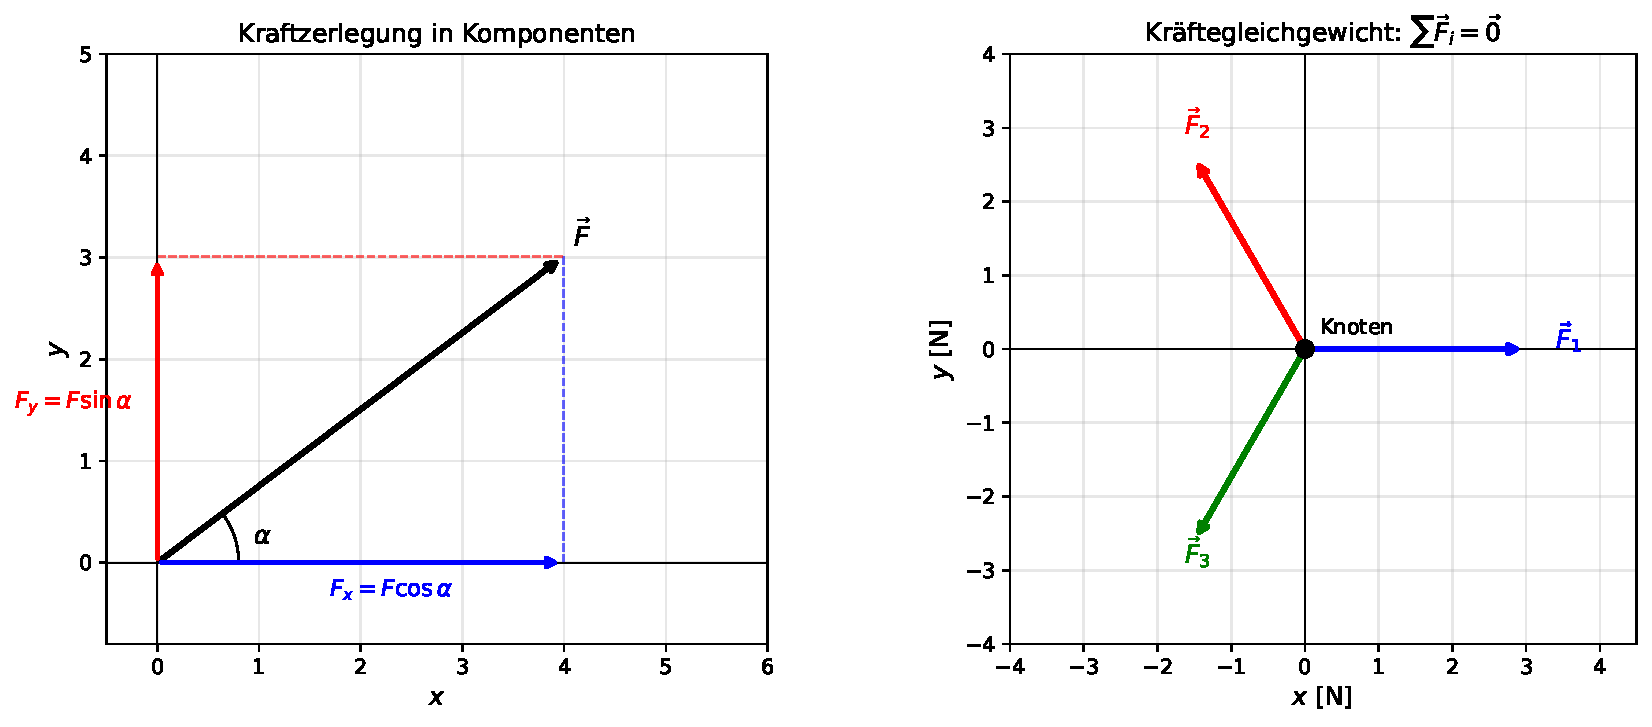
\includegraphics[width=0.92\textwidth]{plot_statik.pdf}
\caption{Links: Zerlegung einer Kraft $\vec{F} = 5\,\mathrm{kN}$ unter $\alpha = 37^\circ$
in Komponenten $F_x$ (blau) und $F_y$ (rot).
Rechts: Drei Kr\"afte im Gleichgewicht -- die Vektorsumme
$\vec{F}_1 + \vec{F}_2 + \vec{F}_3 = \vec{0}$ ist erf\"ullt.}
\label{fig:statik}
\end{figure}

\begin{satz}[Eindeutigkeit bei statisch bestimmten Systemen]
Ein ebenes, statisch bestimmtes Tragwerk besitzt genau drei unbekannte
Auflagerreaktionen. Die drei Gleichgewichtsbedingungen
\eqref{eq:GGx}--\eqref{eq:GGM} bilden ein eindeutig l\"osbares
lineares Gleichungssystem, sofern die Koeffizientenmatrix regul\"ar ist.
\end{satz}
\begin{proof}
Die Koeffizientenmatrix $\mathbf{A} \in \mathbb{R}^{3\times 3}$ ist genau
dann regul\"ar (det $\mathbf{A} \neq 0$), wenn keine Lagerentsprechungslinien
durch einen gemeinsamen Punkt verlaufen (kinematische Bestimmtheit).
Dann folgt eindeutige L\"osbarkeit aus dem regul\"aren Gleichungssystem.
\end{proof}

\section{Auflagertypen und Lagerreaktionen}

\begin{definition}[Lagerarten im ebenen System]
\begin{itemize}
    \item[-] \textbf{Loslager (Gelenklager)}: verhindert Verschiebung in einer Richtung
          (1 Reaktionskraft, senkrecht zur Lagerf\"uhrung);
          1 Wertigkeit -- ein Freiheitsgrad gebunden
    \item[-] \textbf{Festlager (Gelenklager mit Festlegung)}: verhindert jede Verschiebung
          (2 Reaktionskr\"afte in $x$- und $y$-Richtung);
          2 Wertigkeiten
    \item[-] \textbf{Einspannung (Eingemauert)}: verhindert Verschiebung und Verdrehung
          (2 Reaktionskr\"afte + 1 Reaktionsmoment);
          3 Wertigkeiten
    \item[-] \textbf{Pendel- oder Stab}: \"ubertr\"agt nur Kraft in Stabrichtung (1 Reaktionskraft)
\end{itemize}
Ein System hei\ss{}t \textbf{statisch bestimmt}, wenn die Zahl der Unbekannten
der Zahl der Gleichgewichtsbedingungen entspricht.
\end{definition}

\begin{beispiel}[Zweifeldtr\"ager mit Einzellast]
Ein Balken ($L = 6\,\mathrm{m}$) liegt auf einem Festlager ($A$, $x = 0$)
und einem Loslager ($B$, $x = 6\,\mathrm{m}$). Eine Einzellast $F = 24\,\mathrm{kN}$
greift bei $x = 2\,\mathrm{m}$ an.

\medskip\noindent\textbf{Momentengleichgewicht um $A$}:
\[
  \sum M^{(A)} = 0: \quad F\cdot 2 - B_y\cdot 6 = 0
  \implies B_y = \frac{24\cdot 2}{6} = 8\,\mathrm{kN}.
\]
\textbf{Kraftgleichgewicht in $y$}:
\[
  A_y + B_y - F = 0 \implies A_y = 24 - 8 = 16\,\mathrm{kN}.
\]
\textbf{Kraftgleichgewicht in $x$}: $A_x = 0$ (keine horizontale Last).

Die Last liegt n\"aher an $A$, daher ist $A_y > B_y$. $\square$
\end{beispiel}

\begin{beispiel}[Kragarm mit Streckenlast]
Ein Kragarm ($L = 3\,\mathrm{m}$, Einspannung bei $x = 0$) tr\"agt eine
gleichm\"a\ss{}ig verteilte Last $q = 10\,\mathrm{kN/m}$.
Resultierende der Streckenlast: $F_{\text{res}} = q\cdot L = 30\,\mathrm{kN}$,
Angriffspunkt: Mitte des Balkens bei $x = 1{,}5\,\mathrm{m}$.

\medskip\noindent\textbf{Gleichgewicht}:
\[
  A_y = q\cdot L = 30\,\mathrm{kN}, \quad
  M_A = q\cdot L \cdot \frac{L}{2} = 10\cdot 3\cdot 1{,}5 = 45\,\mathrm{kNm}.
\]
Das Einspannmoment wirkt entgegen der Uhrzeigerrichtung,
um die Rotation durch die Streckenlast zu verhindern. $\square$
\end{beispiel}

\section{Schwerpunkt und Massentr\"agheit}

\begin{definition}[Schwerpunkt eines K\"orpers]
Der \textbf{Schwerpunkt} (Massenmittelpunkt) $S = (x_S, y_S, z_S)$
eines K\"orpers mit Dichte $\rho(\vec{r})$ und Gesamtmasse
$m = \int_V \rho\,\mathrm{d}V$ ist definiert durch:
\[
  \vec{r}_S = \frac{1}{m}\int_V \vec{r}\,\rho(\vec{r})\,\mathrm{d}V.
\]
F\"ur \textbf{homogene K\"orper} ($\rho = \mathrm{const}$) ist
$\vec{r}_S = \frac{1}{V}\int_V \vec{r}\,\mathrm{d}V$ (geometrischer Schwerpunkt).
F\"ur zusammengesetzte K\"orper aus Teilk\"orpern $k$:
\[
  x_S = \frac{\sum_k m_k x_{S,k}}{\sum_k m_k}, \quad
  y_S = \frac{\sum_k m_k y_{S,k}}{\sum_k m_k}.
\]
\end{definition}

\begin{beispiel}[Schwerpunkt eines zusammengesetzten Querschnitts]
Ein T-Querschnitt besteht aus:
Flansch ($b_1 = 200\,\mathrm{mm}$, $h_1 = 20\,\mathrm{mm}$,
Schwerpunkt bei $y_1 = 10\,\mathrm{mm}$ von unten)
und Steg ($b_2 = 20\,\mathrm{mm}$, $h_2 = 180\,\mathrm{mm}$,
Schwerpunkt bei $y_2 = 20 + 90 = 110\,\mathrm{mm}$).
Fl\"achen: $A_1 = 4000\,\mathrm{mm^2}$, $A_2 = 3600\,\mathrm{mm^2}$.
\[
  y_S = \frac{A_1 y_1 + A_2 y_2}{A_1 + A_2}
      = \frac{4000\cdot 10 + 3600\cdot 110}{4000 + 3600}
      = \frac{40000 + 396000}{7600} \approx 57{,}4\,\mathrm{mm}.
\]
\end{beispiel}

\begin{satz}[Steiner'scher Anteil -- Parallelachsentheorem]
Ist $I_{yS}$ das Fl\"achentr\"agheitsmoment einer Querschnittsfl\"ache $A$
bez\"uglich der schwerpunktdurchgehenden $y_S$-Achse, und $I_y$ das Moment
bez\"uglich einer dazu parallelen Achse im Abstand $a$, dann gilt:
\[
  I_y = I_{yS} + A \cdot a^2.
\]
\end{satz}
\begin{proof}
Mit $y' = y + a$ (Koordinate bez\"uglich der verschobenen Achse):
\[
  I_y = \int_A (y')^2\,\mathrm{d}A = \int_A(y+a)^2\,\mathrm{d}A
  = \int_A y^2\,\mathrm{d}A + 2a\underbrace{\int_A y\,\mathrm{d}A}_{=0} + a^2\int_A\mathrm{d}A
  = I_{yS} + Aa^2.
\]
Das mittlere Integral verschwindet, da $y$ auf die Schwerpunktachse bezogen ist.
\end{proof}

\begin{beispiel}[Fl\"achentr\"agheitsmoment des T-Querschnitts]
Mit den Daten aus dem vorigen Beispiel und $y_S \approx 57{,}4\,\mathrm{mm}$:
\[
  I_{S,\text{Flansch}} = \frac{b_1 h_1^3}{12} + A_1(y_1 - y_S)^2
  = \frac{200\cdot20^3}{12} + 4000\cdot(10-57{,}4)^2 \approx 8{,}99\cdot10^6\,\mathrm{mm^4}.
\]
\[
  I_{S,\text{Steg}} = \frac{b_2 h_2^3}{12} + A_2(y_2 - y_S)^2
  = \frac{20\cdot180^3}{12} + 3600\cdot(110-57{,}4)^2 \approx 19{,}60\cdot10^6\,\mathrm{mm^4}.
\]
Gesamt: $I_S \approx 28{,}59\cdot10^6\,\mathrm{mm^4}$.
\end{beispiel}

\section{Fl\"achentr\"agheitsmomente wichtiger Querschnitte}

\begin{definition}[Axiale und polare Fl\"achentr\"agheitsmomente]
Das \textbf{axiale Fl\"achentr\"agheitsmoment} bez\"uglich der $y$-Achse:
\[
  I_y = \int_A z^2\,\mathrm{d}A, \qquad I_z = \int_A y^2\,\mathrm{d}A.
\]
Das \textbf{polare Fl\"achentr\"agheitsmoment} (f\"ur Torsion):
\[
  I_p = \int_A r^2\,\mathrm{d}A = I_y + I_z.
\]
Das \textbf{Widerstandsmoment}: $W_y = I_y / z_{\max}$ (Ma\ss{} f\"ur Biegefestigkeit).
\end{definition}

\begin{center}
\begin{tabular}{lll}
\toprule
Querschnitt & $I_y$ & $W_y$ \\
\midrule
Rechteck ($b \times h$) & $bh^3/12$ & $bh^2/6$ \\
Kreis ($d$) & $\pi d^4/64$ & $\pi d^3/32$ \\
Hohlkreis ($d_a, d_i$) & $\pi(d_a^4 - d_i^4)/64$ & $\pi(d_a^4-d_i^4)/(32 d_a)$ \\
Gleichseitiges Dreieck ($a$) & $a^4\sqrt{3}/96$ & $a^3\sqrt{3}/48$ \\
\bottomrule
\end{tabular}
\end{center}

\section{Statik ebener Fachwerke}

\begin{definition}[Ebenes Fachwerk]
Ein \textbf{ebenes Fachwerk} besteht aus geraden St\"aben, die in
\textbf{Knoten} gelenkig verbunden sind. \"Au\ss{}ere Kr\"afte wirken
nur an den Knoten. Jeder Stab ist daher ein \textbf{Zweikraft-Glied}
und wird nur durch Normalkraft beansprucht (Zug: positiv, Druck: negativ).

Bedingung f\"ur statische Bestimmtheit:
\[
  m = 2k - 3,
\]
wobei $m$ die Stabanzahl und $k$ die Knotenanzahl ist.
\end{definition}

\begin{satz}[Ritter'sches Schnittverfahren]
An einem beliebigen Schnitt durch ein Fachwerk, der h\"ochstens drei
Stabnormalkr\"afte schneidet, k\"onnen die Stabkr\"afte direkt aus
den drei Gleichgewichtsbedingungen f\"ur einen Teilk\"orper bestimmt werden.
\end{satz}
\begin{proof}
Da der Schnitt genau drei unbekannte Stabkr\"afte freilegt und drei
Gleichgewichtsbedingungen vorliegen ($\sum F_x = \sum F_y = \sum M_A = 0$),
entsteht ein eindeutig l\"osbares $3\times 3$-System.
Clevere Wahl des Momentenpunkts $A$ (Schnittpunkt zweier geschnittener Stab-Wirkungslinien)
macht deren Momente null und liefert sofort die dritte Stabkraft.
\end{proof}

\section{Reibungslehre}

\begin{definition}[Coulomb'sche Reibungsgesetze]
An einer Kontaktfl\"ache mit Normalkraft $F_N$ und Reibungskoeffizienten
$\mu_H$ (Haften) bzw. $\mu_G$ (Gleiten):
\begin{itemize}
    \item[-] \textbf{Haftbedingung}: $F_R \le \mu_H F_N$ (K\"orper bleibt in Ruhe)
    \item[-] \textbf{Gleitreibung}: $F_R = \mu_G F_N$, $\mu_G < \mu_H$ (K\"orper gleitet)
    \item[-] Die Reibungskraft wirkt \textbf{entgegen} der Bewegungsrichtung
    \item[-] $F_R$ ist unabh\"angig von der Kontaktfl\"ache (Amontons-Gesetz)
\end{itemize}
Typische Werte: Stahl auf Stahl trocken $\mu_H \approx 0{,}15\ldots0{,}20$,
Stahl auf Stahl ge\"olt $\mu_H \approx 0{,}05\ldots0{,}10$.
\end{definition}

\begin{beispiel}[Schiefe Ebene mit Reibung]
Ein Quader ($m = 80\,\mathrm{kg}$) auf einer schiefen Ebene
($\alpha = 25^\circ$, $\mu_H = 0{,}40$). Gleitet er?
\[
  F_{\parallel} = mg\sin\alpha = 80\cdot9{,}81\cdot\sin25^\circ \approx 331{,}8\,\mathrm{N}.
\]
\[
  F_{N} = mg\cos\alpha = 80\cdot9{,}81\cdot\cos25^\circ \approx 711{,}6\,\mathrm{N}.
\]
\[
  F_{H,\max} = \mu_H\cdot F_N = 0{,}40\cdot711{,}6 \approx 284{,}6\,\mathrm{N}.
\]
Da $F_{\parallel} = 331{,}8\,\mathrm{N} > F_{H,\max} = 284{,}6\,\mathrm{N}$, gleitet der K\"orper.
Der Gleitreibungskoeffizient $\mu_G \approx 0{,}32$ (falls gegeben)
liefert die Bremsraft $F_G = 0{,}32\cdot711{,}6 = 227{,}7\,\mathrm{N}$.
\end{beispiel}

% ============================================================
\chapter{Kinematik und Dynamik}
% ============================================================

Kinematik und Dynamik bilden zusammen die \textbf{Mechanik bewegter K\"orper}.
Die Kinematik beschreibt \emph{wie} sich K\"orper bewegen, ohne Ursachen
zu betrachten. Die Dynamik fragt \emph{warum} -- sie verkn\"upft Bewegung
mit Kr\"aften und Momenten. Beide Gebiete sind untrennbar mit der
Differential- und Integralrechnung verkn\"upft.

\section{Kinematik der Punktmasse}

\begin{definition}[Kinematische Grundgr\"o\ss{}en]
Die Bewegung eines Punktes im $\mathbb{R}^3$ wird vollst\"andig durch
den \textbf{Ortsvektor} $\vec{r}(t)$ als Funktion der Zeit beschrieben.
Daraus abgeleitet:
\begin{itemize}
    \item[-] \textbf{Geschwindigkeit}: $\vec{v}(t) = \dot{\vec{r}}(t) = \dfrac{\mathrm{d}\vec{r}}{\mathrm{d}t}$,
          $[\vec{v}] = \mathrm{m/s}$
    \item[-] \textbf{Beschleunigung}: $\vec{a}(t) = \dot{\vec{v}}(t) = \ddot{\vec{r}}(t)$,
          $[\vec{a}] = \mathrm{m/s^2}$
    \item[-] \textbf{Zur\"uckgelegter Weg}: $s = \int_{t_1}^{t_2}|\vec{v}(t)|\,\mathrm{d}t$
\end{itemize}
\end{definition}

\begin{definition}[Gleichm\"a\ss{}ig beschleunigte Bewegung]
Bei konstanter Beschleunigung $\vec{a} = \vec{a}_0 = \mathrm{const}$ gelten
die \textbf{kinematischen Grundformeln} (SUVAT-Gleichungen):
\begin{align}
  \vec{v}(t) &= \vec{v}_0 + \vec{a}_0\,t, \\
  \vec{r}(t) &= \vec{r}_0 + \vec{v}_0\,t + \tfrac{1}{2}\,\vec{a}_0\,t^2, \\
  v^2 &= v_0^2 + 2\,\vec{a}_0 \cdot (\vec{r} - \vec{r}_0).
\end{align}
\end{definition}
\begin{proof}
Integration von $\vec{a}(t) = \vec{a}_0$:
$\vec{v}(t) = \vec{v}_0 + \vec{a}_0 t$.
Nochmalige Integration: $\vec{r}(t) = \vec{r}_0 + \vec{v}_0 t + \tfrac{1}{2}\vec{a}_0 t^2$.
F\"ur die dritte Gleichung wird $t$ aus der ersten Gleichung eliminiert:
$t = (v - v_0)/a_0$ (eindimensional), einsetzen in die zweite:
$s = v_0\cdot\frac{v-v_0}{a_0} + \frac{a_0}{2}\left(\frac{v-v_0}{a_0}\right)^2
= \frac{v^2 - v_0^2}{2a_0}$, also $v^2 = v_0^2 + 2a_0 s$.
\end{proof}

\begin{figure}[htbp]
\centering
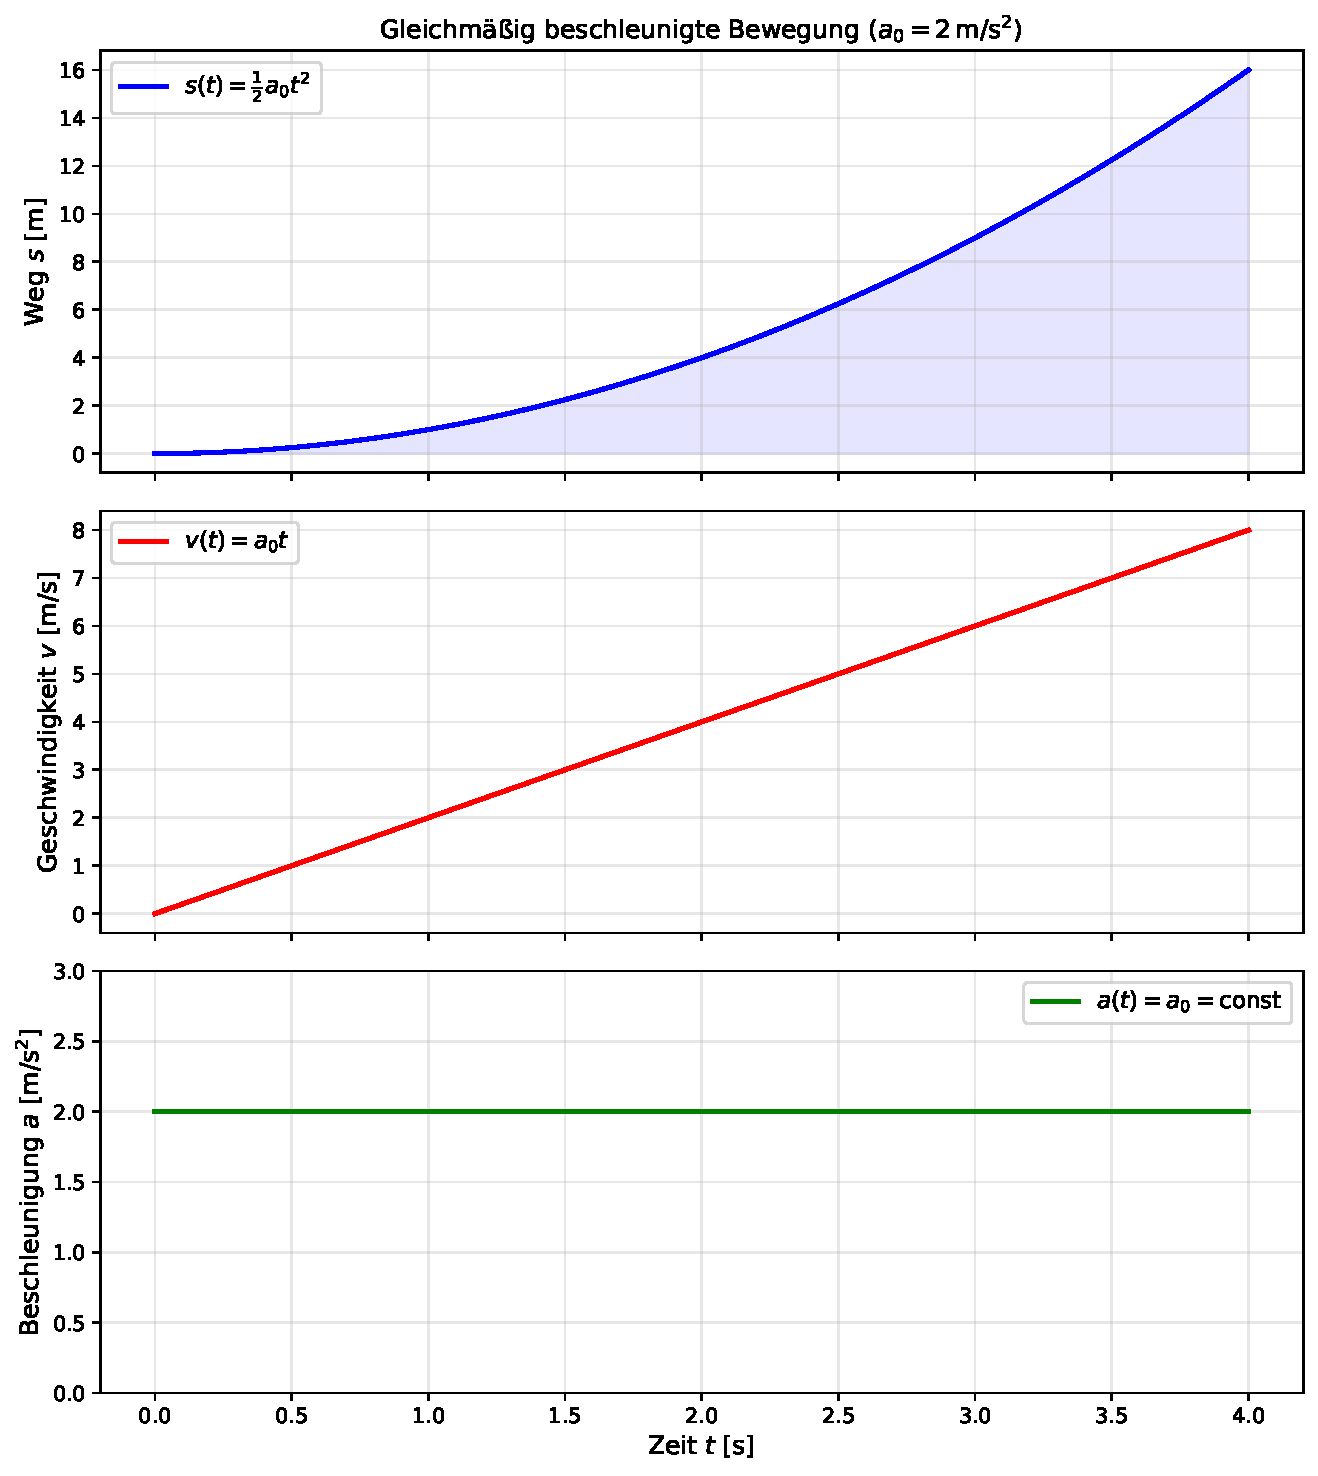
\includegraphics[width=0.75\textwidth]{plot_kinematik.pdf}
\caption{Gleichm\"a\ss{}ig beschleunigte Bewegung mit $a_0 = 2\,\mathrm{m/s^2}$:
Weg $s(t) = \tfrac{1}{2}a_0 t^2$ (Parabel, oben), Geschwindigkeit $v(t) = a_0 t$
(Gerade, Mitte) und konstante Beschleunigung $a(t) = a_0$ (unten).
Die Fl\"ache unter $v(t)$ im Intervall $[t_1, t_2]$ entspricht dem Weg $s(t_2) - s(t_1)$.}
\label{fig:kinematik}
\end{figure}

\begin{beispiel}[Bremsweg eines Fahrzeugs]
Ein PKW f\"ahrt mit $v_0 = 100\,\mathrm{km/h} = 27{,}78\,\mathrm{m/s}$.
Der maximale Bremsverz\"ogerung betr\"agt $a = -8\,\mathrm{m/s^2}$ (trockene Stra\ss{}e).
Zeit bis zum Stillstand: $t = v_0/|a| = 27{,}78/8 \approx 3{,}47\,\mathrm{s}$.
Bremsweg:
\[
  s = \frac{v_0^2}{2|a|} = \frac{27{,}78^2}{2\cdot8} = \frac{771{,}7}{16} \approx 48{,}2\,\mathrm{m}.
\]
Bei nasser Fahrbahn ($a = -4\,\mathrm{m/s^2}$): $s \approx 96{,}5\,\mathrm{m}$ -- doppelt so lang!
\end{beispiel}

\begin{definition}[Schiefer Wurf]
Ein K\"orper wird unter dem Winkel $\alpha_0$ mit der Anfangsgeschwindigkeit $v_0$
abgeworfen. Die Bewegung zerlegts ich in eine gleichf\"ormige horizontale
und eine gleichm\"a\ss{}ig verzögerte (Erdbeschleunigung $g = 9{,}81\,\mathrm{m/s^2}$)
vertikale Komponente:
\begin{align*}
  x(t) &= v_0\cos\alpha_0\cdot t, \\
  y(t) &= v_0\sin\alpha_0\cdot t - \tfrac{1}{2}g t^2.
\end{align*}
Elimination von $t$ ergibt die \textbf{Wurfparabel}:
$y = x\tan\alpha_0 - \dfrac{g}{2v_0^2\cos^2\alpha_0}\,x^2$.
\end{definition}

\begin{satz}[Maximale Wurfweite]
Der schiefe Wurf erreicht die maximale horizontale Wurfweite
\[
  x_{\max} = \frac{v_0^2}{g}
\]
beim Wurfwinkel $\alpha_0 = 45^\circ$.
\end{satz}
\begin{proof}
Die Wurfweite ist $x_W = x(t^*)$ wobei $t^*$ den Zeitpunkt mit $y(t^*) = 0$ angibt:
$t^* = 2v_0\sin\alpha_0/g$.
Einsetzen: $x_W = v_0\cos\alpha_0 \cdot \frac{2v_0\sin\alpha_0}{g}
= \frac{v_0^2\sin 2\alpha_0}{g}$.
Maximierung: $\sin 2\alpha_0 = 1 \Leftrightarrow 2\alpha_0 = 90^\circ \Leftrightarrow \alpha_0 = 45^\circ$,
$x_{\max} = v_0^2/g$.
\end{proof}

\section{Kinematik der Kreisbewegung}

\begin{definition}[Kreisbewegung -- kinematische Gr\"o\ss{}en]
Bei einer Bewegung auf einem Kreis mit Radius $r$ sind die kinematischen
Gr\"o\ss{}en durch den Drehwinkel $\varphi(t)$ ausgedr\"uckt:
\begin{itemize}
    \item[-] \textbf{Winkelgeschwindigkeit}: $\omega = \dot{\varphi}$ in $\mathrm{rad/s}$
    \item[-] \textbf{Winkelbeschleunigung}: $\varepsilon = \dot{\omega} = \ddot{\varphi}$ in $\mathrm{rad/s^2}$
    \item[-] \textbf{Bahngeschwindigkeit}: $v = r\,\omega$
    \item[-] \textbf{Zentripetalbeschleunigung}: $a_z = r\,\omega^2 = v^2/r$ (nach innen gerichtet)
    \item[-] \textbf{Tangentialbeschleunigung}: $a_t = r\,\varepsilon$ (tangential)
    \item[-] \textbf{Gesamtbeschleunigung}: $a = \sqrt{a_z^2 + a_t^2}$
\end{itemize}
Umrechnungen: $n\,[\mathrm{min^{-1}}] = \omega/(2\pi)\cdot 60$; $T = 2\pi/\omega$ (Umlaufdauer).
\end{definition}

\begin{beispiel}[Autorad und Zentripetalbeschleunigung]
Ein Autorad mit $r = 0{,}32\,\mathrm{m}$ dreht bei $v = 120\,\mathrm{km/h} = 33{,}3\,\mathrm{m/s}$:
\[
  \omega = \frac{v}{r} = \frac{33{,}3}{0{,}32} \approx 104{,}2\,\mathrm{rad/s}, \quad
  n = \frac{\omega\cdot 60}{2\pi} \approx 995\,\mathrm{min^{-1}}.
\]
Die Zentripetalbeschleunigung am \"au\ss{}ersten Punkt des Reifens:
$a_z = r\omega^2 = 0{,}32\cdot104{,}2^2 \approx 3474\,\mathrm{m/s^2} \approx 354\,g$.
\end{beispiel}

\section{Newtonsche Dynamik}

\begin{satz}[Newtonsche Axiome]
\begin{itemize}
    \item[-] \textbf{1. Axiom -- Tr\"agheitsprinzip}: Jeder K\"orper bleibt in Ruhe
          oder gleichf\"ormig-geradliniger Bewegung, solange keine \"au\ss{}ere Kraft
          auf ihn wirkt: $\vec{F} = \vec{0} \Rightarrow \vec{v} = \mathrm{const}$.
    \item[-] \textbf{2. Axiom -- Grundgesetz der Dynamik}: Die zeitliche \"Anderung
          des Impulses $\vec{p} = m\vec{v}$ ist gleich der Resultierenden aller
          eingr\"undenden Kr\"afte:
          \[
            \vec{F} = \frac{\mathrm{d}\vec{p}}{\mathrm{d}t} = m\,\vec{a}
            \quad \text{(f\"ur } m = \mathrm{const}\text{)}.
          \]
    \item[-] \textbf{3. Axiom -- Actio-Reactio}: Wirkt K\"orper~1 eine Kraft
          $\vec{F}_{12}$ auf K\"orper~2 aus, so wirkt gleichzeitig eine gleich
          gro\ss{}e, entgegengerichtete Kraft $\vec{F}_{21} = -\vec{F}_{12}$ von
          K\"orper~2 auf K\"orper~1.
\end{itemize}
\end{satz}

\begin{satz}[Impulssatz und Impulserhaltung]
Der \textbf{Gesamtimpuls} eines abgeschlossenen Systems (ohne \"au\ss{}ere Kr\"afte)
ist zeitlich konstant:
\[
  \vec{p}_{\text{ges}} = \sum_i m_i \vec{v}_i = \mathrm{const}.
\]
Bei einem geraden zentrischen Sto\ss{} zweier K\"orper ($m_1, v_1, m_2, v_2$):
\[
  m_1 v_1 + m_2 v_2 = m_1 v_1' + m_2 v_2' \quad (\text{Impulssatz}).
\]
Zus\"atzlich beim elastischen Sto\ss{}: Energieerhaltung
$\tfrac{1}{2}m_1 v_1^2 + \tfrac{1}{2}m_2 v_2^2 = \tfrac{1}{2}m_1 v_1'^2 + \tfrac{1}{2}m_2 v_2'^2$.
\end{satz}
\begin{proof}
Impulserhaltung: $\dot{\vec{p}}_{\text{ges}} = \sum_i m_i \vec{a}_i
= \sum_i \vec{F}_i^{\text{ext}} + \sum_{i\neq j}\vec{F}_{ij}$.
Die inneren Kr\"afte heben sich paarweise auf (3. Axiom): $\vec{F}_{ij} + \vec{F}_{ji} = 0$.
Somit $\dot{\vec{p}}_{\text{ges}} = \vec{F}^{\text{ext}}_{\text{ges}}$.
F\"ur $\vec{F}^{\text{ext}}_{\text{ges}} = 0$ folgt $\vec{p}_{\text{ges}} = \mathrm{const}$.
\end{proof}

\begin{satz}[Energiesatz der Mechanik]
Die \textbf{kinetische Energie} einer Punktmasse ist $E_k = \tfrac{1}{2}mv^2$.
In einem konservativen Kraftfeld (Gradient einer potentiellen Energie $U$:
$\vec{F} = -\nabla U$) gilt der \textbf{Energieerhaltungssatz}:
\[
  E_k + U = \mathrm{const}, \qquad \tfrac{1}{2}mv^2 + U = \mathrm{const}.
\]
Wichtige Sonderf\"alle:
\begin{itemize}
    \item[-] \textbf{Schwerefeld}: $U = mgh$ (Gravitation nahe Erdoberfl\"ache)
    \item[-] \textbf{Federfeld}: $U = \tfrac{1}{2}cx^2$ (Hooke)
    \item[-] \textbf{Koulombfeld}: $U = kQq/r$ (Elektrostatik)
\end{itemize}
\end{satz}
\begin{proof}
$\frac{\mathrm{d}}{\mathrm{d}t}(E_k + U) = m\vec{v}\cdot\vec{a} + \dot{U}
= \vec{v}\cdot(m\vec{a}) + \nabla U \cdot \vec{v}
= \vec{v}\cdot\vec{F} + (-\vec{F})\cdot\vec{v} = 0$.
\end{proof}

\section{Drehmechanik des starren K\"orpers}

\begin{definition}[Massentr\"agheitsmoment]
Das \textbf{Massentr\"agheitsmoment} $J$ eines K\"orpers bez\"uglich
einer Drehachse $\Delta$ ist:
\[
  J = \int_V r^2\,\mathrm{d}m = \int_V r^2\,\rho(\vec{r})\,\mathrm{d}V,
\]
wobei $r$ der senkrechte Abstand des Massenelements $\mathrm{d}m$ von $\Delta$ ist.
Einheit: $[J] = \mathrm{kg\,m^2}$.
\end{definition}

\begin{satz}[Steiner'scher Anteil -- Massentr\"agheitsmoment]
Ist $J_S$ das Massentr\"agheitsmoment bez\"uglich einer Achse durch den
Schwerpunkt $S$ und $J_A$ bez\"uglich einer dazu parallelen Achse im Abstand $a$:
\[
  J_A = J_S + m\,a^2.
\]
\end{satz}
\begin{proof}
Analog zum Steiner'schen Anteil f\"ur Fl\"achentr\"agheitsmomente:
$J_A = \int r_A^2\,\mathrm{d}m = \int(r_S + a)^2\,\mathrm{d}m$
(vektorielle Zerlegung des Abstands, $r_A^2 = r_S^2 + 2ar_S + a^2$),
der Kreuzterm verschwindet ($\int r_S\,\mathrm{d}m = 0$ per Definition des Schwerpunkts).
\end{proof}

\begin{center}
\begin{tabular}{lll}
\toprule
K\"orper & Achse & $J_S$ \\
\midrule
Zylinder ($m$, $R$) & Symmetrieachse & $\frac{1}{2}mR^2$ \\
Hohlzylinder ($m$, $R_a$, $R_i$) & Symmetrieachse & $\frac{1}{2}m(R_a^2+R_i^2)$ \\
D\"unne Scheibe ($m$, $R$) & Symmetrieachse & $\frac{1}{2}mR^2$ \\
Kugel ($m$, $R$) & Durchmesser & $\frac{2}{5}mR^2$ \\
D\"unner Stab ($m$, $L$) & Mittelpunkt, senkrecht & $\frac{1}{12}mL^2$ \\
D\"unner Stab ($m$, $L$) & Endpunkt, senkrecht & $\frac{1}{3}mL^2$ \\
\bottomrule
\end{tabular}
\end{center}

\begin{beispiel}[Massentr\"agheitsmoment einer Vollscheibe]
Eine Vollscheibe ($m = 5\,\mathrm{kg}$, $R = 0{,}2\,\mathrm{m}$, homogen):
\[
  J_S = \frac{mR^2}{2} = \frac{5 \cdot 0{,}04}{2} = 0{,}1\,\mathrm{kg\,m^2}.
\]
Eine am Rand angebrachte Punktmasse ($m_P = 0{,}5\,\mathrm{kg}$) erh\"oht das
Massentr\"agheitsmoment (Steiner): $J_{P} = m_P R^2 = 0{,}5\cdot0{,}04 = 0{,}02\,\mathrm{kg\,m^2}$.
Gesamtmoment: $J_{\text{ges}} = 0{,}10 + 0{,}02 = 0{,}12\,\mathrm{kg\,m^2}$.
\end{beispiel}

\begin{satz}[Drallsatz (Dreh-Newton)]
Das auf einen K\"orper wirkende \"au\ss{}ere Moment $\vec{M}$ ist gleich
der zeitlichen \"Anderung des Drehimpulses $\vec{L} = J\vec{\omega}$:
\[
  \vec{M} = \dot{\vec{L}} = J\,\dot{\vec{\omega}} = J\,\vec{\varepsilon}.
\]
\end{satz}
\begin{proof}
Der Drallsatz ist das rotatorische \"Aquivalent von $\vec{F} = m\vec{a}$:
F\"ur eine Punktmasse auf Kreisbahn gilt $L = r\,mv = r\,m\,r\,\omega = mr^2\omega$.
Integration \"uber den K\"orper ergibt $L = J\omega$.
Differentiation: $\dot{L} = J\dot{\omega} = J\varepsilon = M$.
\end{proof}

\begin{beispiel}[Anlaufvorgang einer Maschine]
Ein rotierender K\"orper ($J = 2\,\mathrm{kg\,m^2}$) soll von $n_0 = 0$
auf $n = 3000\,\mathrm{min^{-1}}$ in $t = 10\,\mathrm{s}$ beschleunigt werden.
\[
  \omega_{\text{end}} = \frac{2\pi\cdot 3000}{60} = 314{,}2\,\mathrm{rad/s},
  \quad
  \varepsilon = \frac{\Delta\omega}{\Delta t} = \frac{314{,}2}{10} = 31{,}42\,\mathrm{rad/s^2}.
\]
Das erforderliche Anlaufmoment:
\[
  M = J\cdot\varepsilon = 2\cdot31{,}42 = 62{,}8\,\mathrm{Nm}.
\]
Die im Anlauf gespeicherte kinetische Rotationsenergie:
\[
  E_k = \tfrac{1}{2}J\omega^2 = \tfrac{1}{2}\cdot2\cdot314{,}2^2 \approx 98{,}7\,\mathrm{kJ}.
\]
\end{beispiel}

\section{Arbeit, Leistung und Wirkungsgrad}

\begin{definition}[Mechanische Arbeit und Leistung]
Die \textbf{mechanische Arbeit} einer Kraft $\vec{F}$ entlang eines Weges $\mathcal{C}$:
\[
  W = \int_{\mathcal{C}} \vec{F}\,\mathrm{d}\vec{s}.
\]
Die \textbf{Leistung} ist die Arbeit pro Zeit:
\[
  P = \frac{\mathrm{d}W}{\mathrm{d}t} = \vec{F}\cdot\vec{v}.
\]
F\"ur Rotation: $P = M\cdot\omega$.
Der \textbf{Wirkungsgrad} $\eta = P_{\text{nutz}}/P_{\text{zu}}$ gibt an,
welcher Anteil der zugef\"uhrten Leistung nutzbringend umgewandelt wird ($0 < \eta < 1$).
\end{definition}

% ============================================================
\chapter{Festigkeitslehre}
% ============================================================

Die Festigkeitslehre (Elastostatik) untersucht das Verhalten von Bauteilen
unter mechanischer Belastung. Ziel ist die Sicherstellung, dass Spannungen
die Werkstoffgrenzen nicht \"uberschreiten und Verformungen zul\"assige
Ma\ss{}e nicht \"uberschreiten. Sie bildet die wissenschaftliche Grundlage
der gesamten Bauteilauslegung im Maschinenbau.

\section{Spannungszustand und Hookesches Gesetz}

\begin{definition}[Spannungsvektor und Normalspannung]
Auf einem infinitesimalen Querschnittselement $\mathrm{d}A$ wirkt
ein Kraft-Inkrement $\mathrm{d}\vec{F}$. Der \textbf{Spannungsvektor}:
\[
  \vec{t} = \lim_{\mathrm{d}A \to 0}\frac{\mathrm{d}\vec{F}}{\mathrm{d}A}.
\]
Zerlegung in Normalspannung (senkrecht zur Fl\"ache) und Schubspannung (in der Fl\"ache):
\[
  \sigma = \frac{N}{A} \quad [\mathrm{N/mm^2} = \mathrm{MPa}], \qquad
  \tau = \frac{Q}{A} \quad [\mathrm{MPa}].
\]
Vorzeichen: Zugspannung $\sigma > 0$, Druckspannung $\sigma < 0$.
\end{definition}

\begin{definition}[Dehnung und Querkontraktion]
Unter Normalspannung $\sigma$ \"andert sich die L\"ange von $l_0$ auf $l$:
\[
  \varepsilon = \frac{l - l_0}{l_0} = \frac{\Delta l}{l_0} \quad (\text{Dehnung, dimensionslos}).
\]
Gleichzeitig tritt \textbf{Querkontraktion} auf (Poisson-Effekt):
$\varepsilon_q = -\nu\,\varepsilon$, mit der Querdehnungszahl $\nu$
(f\"ur Stahl: $\nu \approx 0{,}3$, f\"ur Gummi: $\nu \approx 0{,}5$).
\end{definition}

\begin{definition}[Hookesches Gesetz -- eindimensional und verallgemeinert]
Im \textbf{linear-elastischen Bereich} gilt proportionaler Zusammenhang:
\[
  \sigma = E\,\varepsilon, \qquad \tau = G\,\gamma,
\]
mit Elastizit\"atsmodul $E$ (f\"ur Stahl: $E \approx 210\,\mathrm{GPa}$;
Aluminium: $E \approx 70\,\mathrm{GPa}$; Titanium: $E \approx 115\,\mathrm{GPa}$)
und Schubmodul:
\[
  G = \frac{E}{2(1+\nu)}.
\]
\end{definition}

\begin{satz}[Dreidimensionaler Spannungszustand -- Hookesches Gesetz]
Im allgemeinen dreidimensionalen Spannungszustand mit Spannungskomponenten
$\sigma_x, \sigma_y, \sigma_z, \tau_{xy}, \tau_{xz}, \tau_{yz}$ gelten
die \textbf{verallgemeinerten Hookeschen Gleichungen}:
\begin{align*}
  \varepsilon_x &= \frac{1}{E}[\sigma_x - \nu(\sigma_y + \sigma_z)], \\
  \varepsilon_y &= \frac{1}{E}[\sigma_y - \nu(\sigma_x + \sigma_z)], \\
  \varepsilon_z &= \frac{1}{E}[\sigma_z - \nu(\sigma_x + \sigma_y)], \\
  \gamma_{xy}   &= \tau_{xy}/G, \quad \gamma_{xz} = \tau_{xz}/G, \quad \gamma_{yz} = \tau_{yz}/G.
\end{align*}
\end{satz}
\begin{proof}
Das Ergebnis folgt aus dem Superpositionsprinzip (Linearit\"at des Hookeschen Gesetzes):
Jede Normalspannung $\sigma_i$ erzeugt eine Dehnung $\sigma_i/E$ in ihrer Richtung
und Querdehnungen $-\nu\sigma_i/E$ in den beiden senkrechten Richtungen.
Summation der Beitr\"age aller drei Normalspannungen ergibt die obigen Gleichungen.
\end{proof}

\begin{figure}[htbp]
\centering
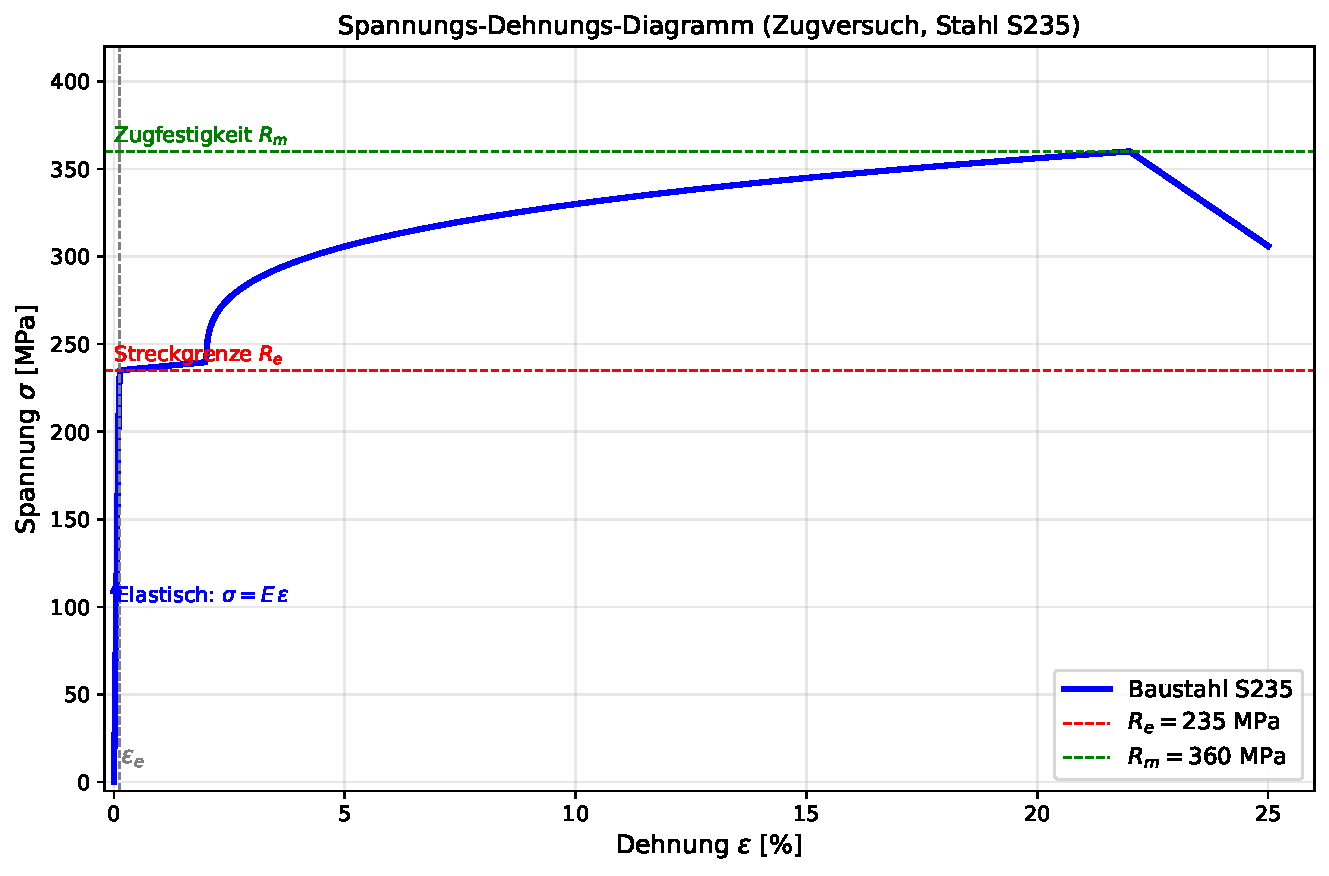
\includegraphics[width=0.82\textwidth]{plot_festigkeit.pdf}
\caption{Spannungs-Dehnungs-Diagramm (Zugversuch, Baustahl S235):
Im elastischen Bereich ($\varepsilon < \varepsilon_e$) gilt $\sigma = E\varepsilon$.
Bei der Streckgrenze $R_e = 235\,\mathrm{MPa}$ setzt plastisches Flie\ss{}en ein.
Die Zugfestigkeit $R_m = 360\,\mathrm{MPa}$ markiert das Spannungsmaximum
vor dem Bruch.}
\label{fig:festigkeit}
\end{figure}

\begin{definition}[Technische Kennwerte aus dem Zugversuch]
\begin{itemize}
    \item[-] \textbf{Streckgrenze} $R_e$ [MPa]: Spannung beim Eintritt plastischen Flie\ss{}ens
    \item[-] \textbf{0{,}2\%-Dehngrenze} $R_{p0,2}$: Spannung, bei der nach Entlastung
          eine bleibende Dehnung von 0{,}2\% verbleibt (f\"ur nicht ausgeprägte Streckgrenze)
    \item[-] \textbf{Zugfestigkeit} $R_m$ [MPa]: maximale Nennspannung im Zugversuch
    \item[-] \textbf{Bruchdehnung} $A$ [\%]: plastische Dehnung bei Bruch
    \item[-] \textbf{Brucheinschn\"urung} $Z$ [\%]: relative Querschnittsabnahme bei Bruch
    \item[-] \textbf{Kerbschlagarbeit} $K_V$ [J]: Schlagz\"ahigkeit (Kerbschlagbiegeversuch)
\end{itemize}
\end{definition}

\begin{satz}[Vergleichsspannung und Festigkeitshypothesen]
Um mehrachsige Spannungszust\"ande mit einachsigen Festigkeitskennwerten
vergleichen zu k\"onnen, werden \textbf{Vergleichsspannungen} berechnet.
Wichtige Hypothesen:
\begin{itemize}
    \item[-] \textbf{Normalspannungshypothese (NH)}: $\sigma_V = \sigma_1$
          (gr\"o\ss{}te Hauptspannung; f\"ur spr\"ode Werkstoffe)
    \item[-] \textbf{Schubspannungshypothese (SH)} (Tresca):
          $\sigma_V = \sigma_1 - \sigma_3$ (f\"ur z\"ahe Metalle unter ruhender Last)
    \item[-] \textbf{Gestalt\"anderungsenergiehypothese (GEH)} (von Mises):
          \[
            \sigma_V = \frac{1}{\sqrt{2}}\sqrt{(\sigma_1-\sigma_2)^2+(\sigma_2-\sigma_3)^2+(\sigma_3-\sigma_1)^2}
          \]
          (genauester f\"ur z\"ahe Metalle; in der Praxis am h\"aufigsten)
\end{itemize}
\end{satz}

\section{Zug, Druck und Biegung}

\begin{definition}[Biegespannung und Biegelinie]
In einem Balken mit \textbf{Biegemoment} $M_b(x)$ und axialem
Fl\"achentr\"agheitsmoment $I_y$ gilt f\"ur die Biegespannung im Abstand $z$
von der neutralen Faser:
\[
  \sigma(z) = \frac{M_b}{I_y}\,z, \qquad
  \sigma_{\max} = \frac{M_b}{I_y}\,z_{\max} = \frac{M_b}{W_y}.
\]
Die \textbf{Biegelinie} $w(x)$ erf\"ullt die DGL:
\[
  EI_y\,w''(x) = -M_b(x), \qquad EI_y\,w^{(4)}(x) = q(x),
\]
wobei $q(x)$ die Streckenlast ist.
\end{definition}

\begin{satz}[Biegelinie des beidseitig aufgelegten Balkens unter Gleichstreckenlast]
F\"ur einen Balken (L\"ange $L$, $EI = \mathrm{const}$) auf zwei Auflagern
($w(0) = w(L) = 0$, $w''(0) = w''(L) = 0$) unter Gleichstreckenlast $q$:
\[
  w(x) = \frac{q}{24EI}(x^4 - 2Lx^3 + L^3 x), \qquad
  w_{\max} = w(L/2) = \frac{5qL^4}{384\,EI}.
\]
\end{satz}
\begin{proof}
Viermalige Integration von $EI w^{(4)} = q$ liefert
$EI w = \frac{q}{24}x^4 + \frac{C_1}{6}x^3 + \frac{C_2}{2}x^2 + C_3 x + C_4$.
Die vier Randbedingungen ($w(0) = w''(0) = w(L) = w''(L) = 0$)
bestimmen: $C_4 = 0$, $C_2 = 0$, $C_3 = qL^3/24$, $C_1 = -qL/2$.
Einsetzen und $w(L/2)$ auswerten liefert das Ergebnis.
\end{proof}

\begin{figure}[htbp]
\centering
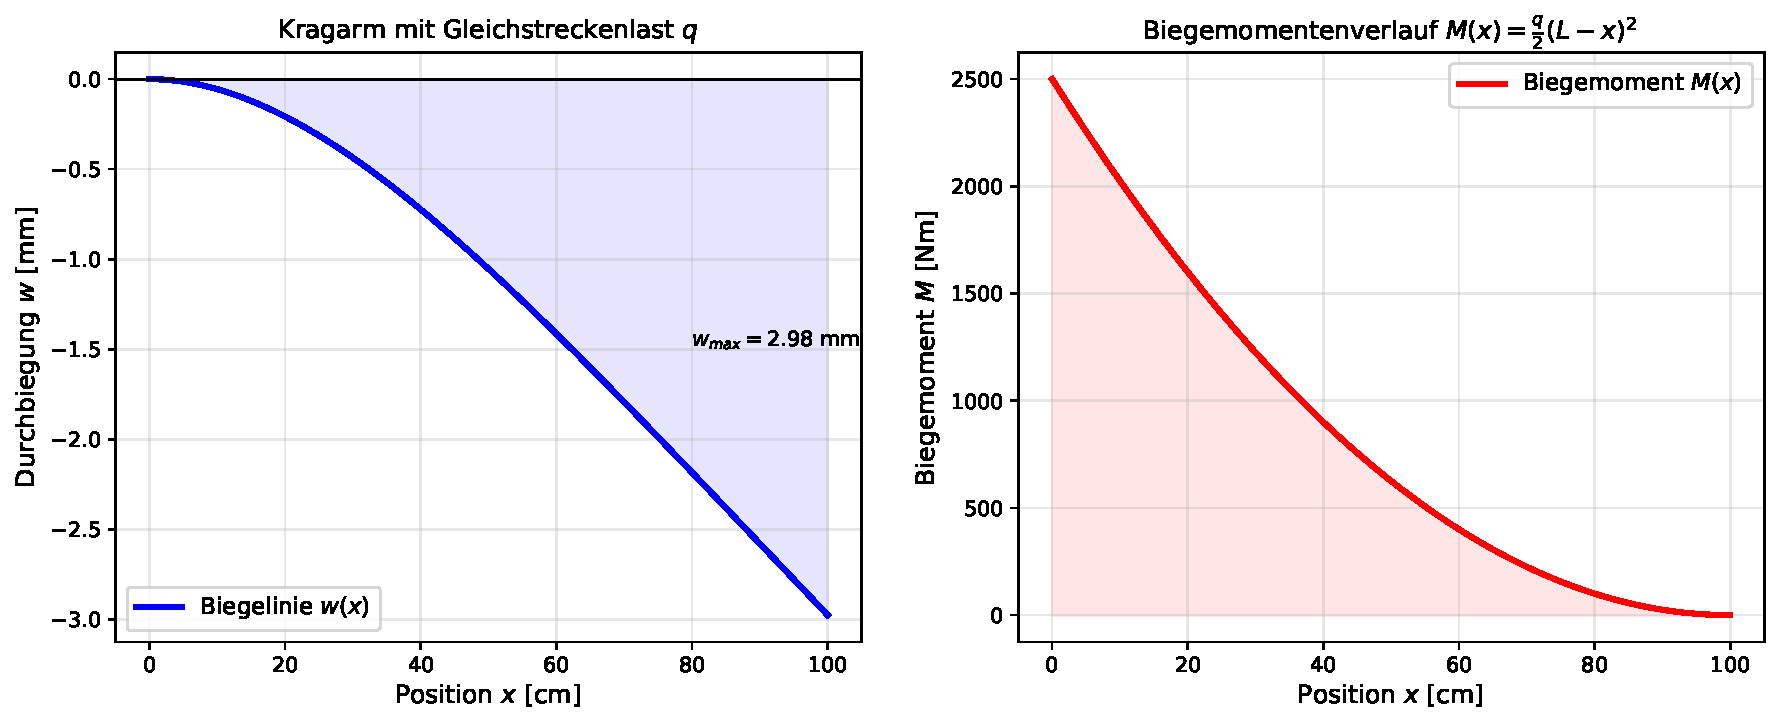
\includegraphics[width=0.92\textwidth]{plot_biegung.pdf}
\caption{Links: Biegelinie $w(x)$ eines Kragarms ($L=1\,\mathrm{m}$, $q = 5\,\mathrm{kN/m}$,
$EI = 210\,\mathrm{kNm^2}$) -- maximale Durchbiegung $w_{\max} = qL^4/(8EI)$ am freien Ende.
Rechts: Biegemomentenverlauf $M(x) = \tfrac{q}{2}(L-x)^2$ -- an der Einspannung maximal,
am freien Ende null.}
\label{fig:biegung}
\end{figure}

\begin{beispiel}[Durchbiegung eines Tr\"agers]
Ein Stahltr\"ager (HEA~200, $I_y = 3692\,\mathrm{cm^4}$, $L = 5\,\mathrm{m}$,
$q = 20\,\mathrm{kN/m}$, $E = 210\,\mathrm{GPa}$):
\[
  w_{\max} = \frac{5qL^4}{384\,EI}
  = \frac{5\cdot20\cdot10^3\cdot5^4}{384\cdot210\cdot10^9\cdot3692\cdot10^{-8}}
  \approx \frac{312{,}5\cdot10^6}{384\cdot77{,}53\cdot10^5} \approx \frac{312{,}5}{2977} \approx 0{,}105\,\mathrm{m}.
\]
Zul\"assige Durchbiegung oft $L/300 = 5000/300 \approx 16{,}7\,\mathrm{mm}$:
Der Tr\"ager ist nicht ausreichend steif -- ein gr\"o\ss{}eres Profil wird ben\"otigt!
\end{beispiel}

\section{Torsion kreisf\"ormiger Querschnitte}

\begin{definition}[Torsionsschubspannung]
Ein Kreisquerschnitt (Radius $R$) unter Torsionsmoment $M_t$ erf\"ahrt die
Schubspannung:
\[
  \tau(r) = \frac{M_t}{I_p}\,r, \qquad
  \tau_{\max} = \frac{M_t}{W_p} = \frac{2M_t}{\pi R^3},
\]
mit dem polaren Fl\"achentr\"agheitsmoment $I_p = \tfrac{\pi}{2}R^4$
und dem polaren Widerstandsmoment $W_p = I_p/R$.
Der \textbf{Drillwinkel} pro L\"angeneinheit:
\[
  \vartheta' = \frac{M_t}{GI_p}.
\]
\end{definition}

\begin{satz}[Maximale Torsionsbelastung von Hohlwellen]
F\"ur eine Hohlwelle ($R_a, R_i$) ist das polare Tr\"agheitsmoment
$I_p = \tfrac{\pi}{2}(R_a^4 - R_i^4)$. Bei gleichem $M_t$ und gleichem $\tau_{\max}$
ben\"otigt eine Hohlwelle weniger Material als eine Vollwelle:
das Verh\"altnis der Massen ist $m_H/m_V = 1 - (R_i/R_a)^2$.
\end{satz}
\begin{proof}
Sei $\tau_{\max} = M_t/W_p = \mathrm{const}$. F\"ur Vollwelle: $W_{p,V} = \pi R_V^3/2$.
F\"ur Hohlwelle: $W_{p,H} = \pi(R_a^4 - R_i^4)/(2R_a)$.
Gleichung $W_{p,H} = W_{p,V}$ legt $R_a$ fest.
Die Masse $m = \rho\pi(R_a^2 - R_i^2)L$ vs. $m_V = \rho\pi R_V^2 L$;
das Verh\"altnis $m_H/m_V < 1$ zeigt die Materialeffizienz der Hohlwelle.
\end{proof}

\begin{beispiel}[Antriebswellenauslegung]
Eine Stahlwelle soll $P = 50\,\mathrm{kW}$ bei $n = 1000\,\mathrm{min^{-1}}$
\"ubertragen. Zul\"assige Torsionsschubspannung $\tau_{zul} = 60\,\mathrm{MPa}$.
\[
  M_t = \frac{P}{\omega} = \frac{50000}{2\pi\cdot1000/60} \approx 477\,\mathrm{Nm}.
\]
Mindest-Wellendurchmesser aus $\tau_{\max} \le \tau_{zul}$:
\[
  W_p = \frac{M_t}{\tau_{zul}} = \frac{477}{60} = 7{,}95\,\mathrm{mm^3}\cdot10^3
  \Rightarrow \frac{\pi d^3}{16} \ge 7950\,\mathrm{mm^3}
  \Rightarrow d \ge \sqrt[3]{\frac{16\cdot7950}{\pi}} \approx 39{,}6\,\mathrm{mm}.
\]
Gew\"ahlt wird $d = 40\,\mathrm{mm}$ (n\"achste Normgr\"o\ss{}e).
\end{beispiel}

\section{Knickung -- Euler'sche Stabknicklast}

\begin{definition}[Stabknicken -- Euler'sche F\"alle]
Ein schlanker druckbelasteter Stab versagt bei Erreichen der \textbf{Knicklast}
$F_{krit}$ durch seitliches Ausweichen (Instabilit\"at).
F\"ur den \textbf{gelenkig gelagerten Stab} (Euler-Fall 2):
\[
  F_{krit} = \frac{\pi^2\,E\,I_{\min}}{l_k^2},
\]
mit der \textbf{Knicklänge} $l_k$ (abh\"angig von den Einspannbedingungen):
\begin{itemize}
    \item[-] Euler-Fall 1 (beidseitig eingespannt): $l_k = L/2$
    \item[-] Euler-Fall 2 (beidseitig gelenkig): $l_k = L$
    \item[-] Euler-Fall 3 (ein Ende eingespannt, ein Ende gelenkig): $l_k = 0{,}7L$
    \item[-] Euler-Fall 4 (ein Ende eingespannt, ein Ende frei): $l_k = 2L$
\end{itemize}
\end{definition}

\begin{satz}[Euler'sche Knicklast -- Herleitung]
F\"ur den gelenkig gelagerten Stab ($l_k = L$) unter Druckkraft $F$
erf\"ullt die Biegelinie die DGL:
$EI\,w'' + F\,w = 0$ mit $w(0) = w(L) = 0$.
Die kleinste nichttriviale L\"osung tritt bei $F = \pi^2 EI/L^2$ auf.
\end{satz}
\begin{proof}
Die DGL $w'' + k^2 w = 0$ mit $k^2 = F/(EI)$ hat die allgemeine L\"osung
$w(x) = A\sin(kx) + B\cos(kx)$.
Aus $w(0) = 0$: $B = 0$. Aus $w(L) = 0$: $A\sin(kL) = 0$.
F\"ur $A \neq 0$ (nichtriviale L\"osung): $kL = n\pi$, $n \in \mathbb{N}$.
Kleinste L\"osung ($n=1$): $k = \pi/L$, also $F_{krit} = k^2 EI = \pi^2 EI/L^2$.
\end{proof}

% ============================================================
\chapter{Str\"omungslehre}
% ============================================================

Die Str\"omungsmechanik (Fluidmechanik) beschreibt die Bewegung von
Fl\"ussigkeiten und Gasen. Im Maschinenbau ist sie grundlegend f\"ur
die Auslegung von Pumpen, Verdichtern, Turbinen, W\"armetauschern,
Rohrleitungssystemen, Fahrzeugen und Flugzeugen.

\section{Fluideigenschaften und Hydrostatik}

\begin{definition}[Fluideigenschaften]
Ein \textbf{Fluid} (Fl\"ussigkeit oder Gas) kann Schubspannungen im
Ruhezustand nicht aufnehmen. Wichtige Eigenschaften:
\begin{itemize}
    \item[-] \textbf{Dichte}: $\rho = m/V$ in $\mathrm{kg/m^3}$
          (Wasser: $\rho_W = 1000\,\mathrm{kg/m^3}$; Luft: $\rho_L \approx 1{,}2\,\mathrm{kg/m^3}$)
    \item[-] \textbf{Dynamische Viskosit\"at}: $\eta$ in $\mathrm{Pa\,s}$
          (Newtonsche Fluide: $\tau = \eta\,\mathrm{d}v/\mathrm{d}y$)
    \item[-] \textbf{Kinematische Viskosit\"at}: $\nu = \eta/\rho$ in $\mathrm{m^2/s}$
    \item[-] \textbf{Kompressibilit\"at}: $\kappa = -(1/V)(\mathrm{d}V/\mathrm{d}p)$
          (Fl\"ussigkeiten: $\kappa \approx 0$; Gase: abh\"angig von Prozess)
\end{itemize}
\end{definition}

\begin{satz}[Hydrostatische Grundgleichung]
Im ruhenden Fluid unter Schwerkraft $g$ gilt f\"ur den Druckverlauf
mit der Tiefe $h$ (nach unten positiv):
\[
  \frac{\mathrm{d}p}{\mathrm{d}h} = \rho g, \qquad p(h) = p_0 + \rho g h.
\]
\end{satz}
\begin{proof}
Betrachte ein Volumenelement $\mathrm{d}V = A\,\mathrm{d}h$.
Gleichgewicht in $h$-Richtung: $(p + \mathrm{d}p)A - p\,A = \rho g\,A\,\mathrm{d}h$,
also $\mathrm{d}p = \rho g\,\mathrm{d}h$. Integration ergibt $p = p_0 + \rho g h$.
\end{proof}

\begin{beispiel}[Wasserdruck in einem Stausee]
In einem Stausee mit $h = 50\,\mathrm{m}$ Tiefe betr\"agt der Wasserdruck
(\"Uberdruck):
\[
  p = \rho g h = 1000\cdot9{,}81\cdot50 = 490\,500\,\mathrm{Pa} \approx 4{,}9\,\mathrm{bar}.
\]
Eine Staumauer muss diesem Druckprofil widerstehen -- die resultierende
horizontale Wasserdruckkraft auf eine Mauer der Breite $B$ und H\"ohe $H$:
$F_H = \tfrac{1}{2}\rho g H^2 B$ (Dreieckslast, Angriffspunkt bei $H/3$ von unten).
\end{beispiel}

\section{Kinematik und Grundgleichungen der Str\"omung}

\begin{definition}[Kontinuit\"atsgleichung]
F\"ur \textbf{inkompressible Str\"omungen} ($\rho = \mathrm{const}$)
ist der Volumenstrom $\dot{V}$ konstant:
\[
  A_1 v_1 = A_2 v_2 = \dot{V} = \mathrm{const}.
\]
F\"ur kompressible Str\"omungen gilt die Massenerhaltung:
$\rho_1 A_1 v_1 = \rho_2 A_2 v_2 = \dot{m} = \mathrm{const}$.
\end{definition}

\begin{satz}[Bernoulligleichung -- Energieerhaltung in Str\"omungen]
F\"ur station\"are, reibungsfreie, inkompressible Str\"omung
entlang einer Stromlinie:
\[
  p + \frac{\rho}{2}v^2 + \rho g z = p_0 = \mathrm{const}.
\]
Die drei Terme sind: statischer Druck $p$, dynamischer Druck (Staudruck)
$q = \frac{\rho}{2}v^2$ und geodätischer Druck $\rho g z$.
\end{satz}
\begin{proof}
Entlang einer Stromlinie gilt $\mathrm{d}\vec{r}/\mathrm{d}s = \vec{v}/v$.
Die Euler'sche Bewegungsgleichung f\"ur reibungsfreie Str\"omung:
$\rho(\vec{v}\cdot\nabla)\vec{v} = -\nabla p - \rho g\vec{e}_z$.
Skalarprodukt mit $\mathrm{d}\vec{r}$ und Integration entlang der Stromlinie:
$\int(\vec{v}\cdot\nabla)\vec{v}\cdot\mathrm{d}\vec{r} = \int v\,\mathrm{d}v = \mathrm{d}(v^2/2)$.
Einsetzen und Integrieren ergibt die Bernoulligleichung.
\end{proof}

\begin{figure}[htbp]
\centering
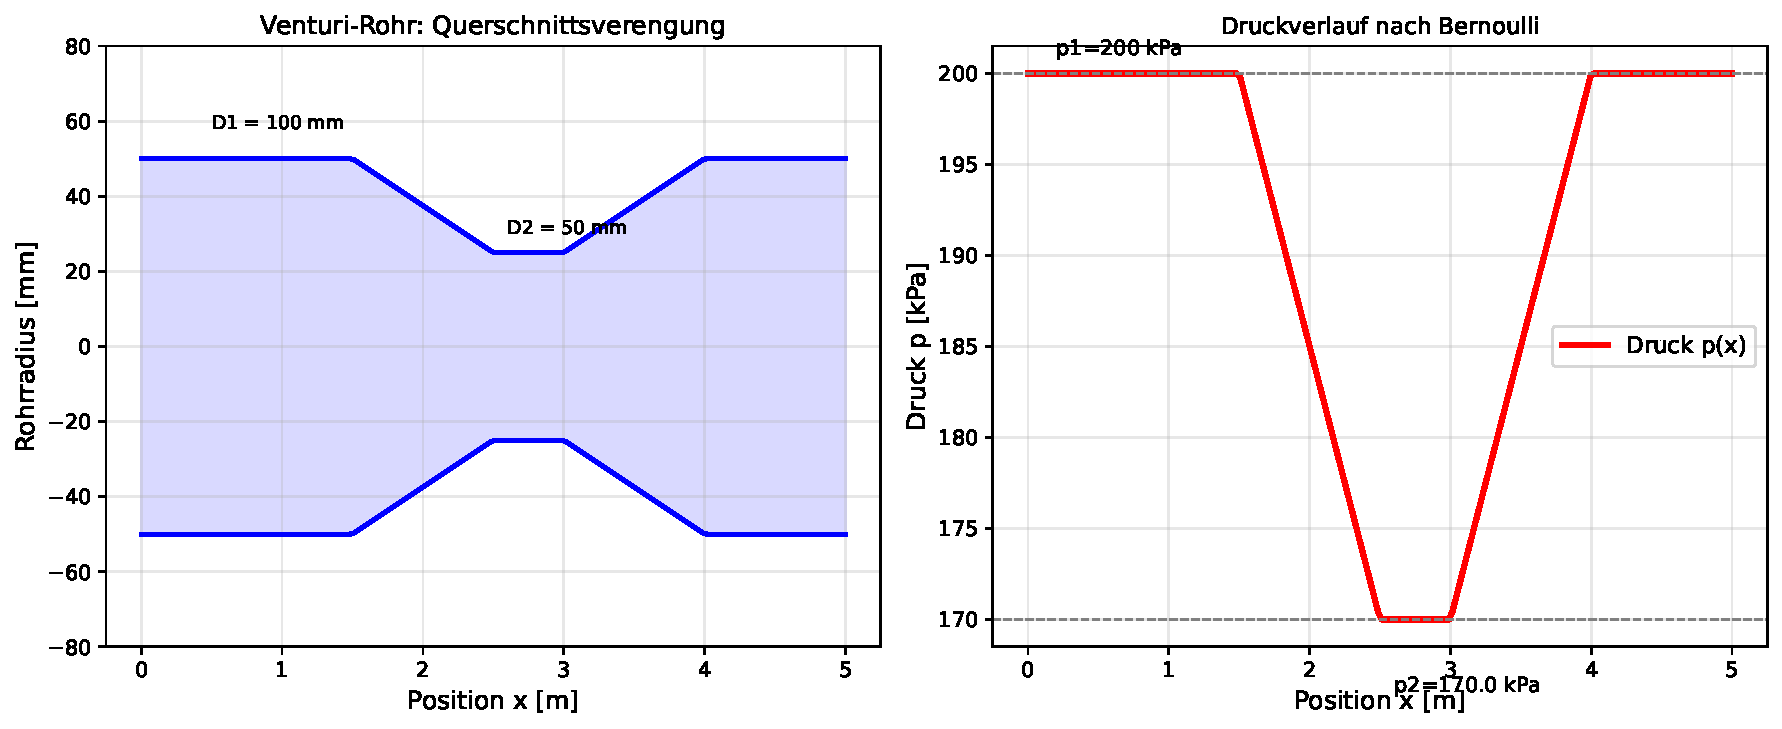
\includegraphics[width=0.92\textwidth]{plot_stroemung.pdf}
\caption{Venturi-Rohr: Links der Querschnittsverlauf (Verengung von $D_1 = 100\,\mathrm{mm}$
auf $D_2 = 50\,\mathrm{mm}$). Rechts der Druckverlauf nach Bernoulli:
Die Beschleunigung des Fluids in der Verengung bewirkt einen Druckabfall
von $p_1 = 200\,\mathrm{kPa}$ auf $p_2 \approx 50\,\mathrm{kPa}$.}
\label{fig:stroemung}
\end{figure}

\begin{beispiel}[Venturi-Durchflussmessung]
Wasser ($\rho = 1000\,\mathrm{kg/m^3}$) str\"omt durch ein Venturi-Rohr
mit $D_1 = 100\,\mathrm{mm}$ und $D_2 = 50\,\mathrm{mm}$.
Gemessene Druckdifferenz $\Delta p = p_1 - p_2 = 30\,\mathrm{kPa}$.
Der Volumenstrom:
\[
  \dot{V} = A_2\sqrt{\frac{2\Delta p/\rho}{1-(A_2/A_1)^2}}
  = \frac{\pi\cdot0{,}05^2}{4}\sqrt{\frac{2\cdot30000/1000}{1-(50/100)^4}}
\]
\[
  \approx 1{,}963\cdot10^{-3}\cdot\sqrt{\frac{60}{1-0{,}0625}}
  \approx 8{,}16\cdot10^{-3}\,\mathrm{m^3/s} = 8{,}16\,\mathrm{l/s}.
\]
\end{beispiel}

\section{Viskose Str\"omungen und Druckverlust}

\begin{definition}[Reynolds-Zahl und Str\"omungsregime]
Die \textbf{Reynolds-Zahl} ist das wichtigste dimensionslose Kennzeichen
zur Charakterisierung einer Str\"omung:
\[
  Re = \frac{v\,L}{\nu} = \frac{\rho\,v\,L}{\eta},
\]
wobei $L$ eine charakteristische L\"ange (z.\,B. Rohrinnendurchmesser $d$) ist.
\begin{itemize}
    \item[-] $Re < 2300$: \textbf{laminare Str\"omung} (geordnete Schichtenstr\"omung)
    \item[-] $2300 < Re < 10^4$: \textbf{\"Ubergangsbereich}
    \item[-] $Re > 10^4$: \textbf{turbulente Str\"omung} (unregelm\"a\ss{}ige Wirbeln)
\end{itemize}
\end{definition}

\begin{satz}[Hagen-Poiseuille -- Laminare Rohrstr\"omung]
F\"ur laminare, viskose, inkompressible Str\"omung in einem geraden Kreisrohr
(Radius $R$, L\"ange $L$, Druckdifferenz $\Delta p$) gilt das parabolische
Geschwindigkeitsprofil:
\[
  v(r) = \frac{\Delta p}{4\eta L}(R^2 - r^2).
\]
Der Volumenstrom (Hagen-Poiseuille-Gesetz):
\[
  \dot{V} = \frac{\pi R^4 \Delta p}{8\eta L} = \frac{\pi d^4 \Delta p}{128\eta L}.
\]
\end{satz}
\begin{proof}
Aus der Navier-Stokes-Gleichung f\"ur station\"are, axialsymmetrische
Str\"omung vereinfacht sich das Momentum-Gleichgewicht zu:
$\frac{1}{r}\frac{\mathrm{d}}{\mathrm{d}r}\left(r\frac{\mathrm{d}v}{\mathrm{d}r}\right) = \frac{\Delta p}{\eta L}$.
Zweifache Integration mit Randbedingungen $v(R) = 0$ (Haftbedingung)
und Regularit\"at bei $r = 0$: $v(r) = \frac{\Delta p}{4\eta L}(R^2 - r^2)$.
Integration \"uber den Querschnitt: $\dot{V} = \int_0^R v(r)\,2\pi r\,\mathrm{d}r
= \frac{\pi\Delta p}{2\eta L}\int_0^R (R^2r - r^3)\,\mathrm{d}r
= \frac{\pi\Delta p}{2\eta L}\cdot\frac{R^4}{4} = \frac{\pi R^4\Delta p}{8\eta L}$.
\end{proof}

\begin{definition}[Druckverlust in Rohrleitungen]
Der Druckverlust durch Rohrreibung wird durch die \textbf{Darcy-Weisbach-Gleichung}
beschrieben:
\[
  \Delta p_V = \lambda\,\frac{L}{d}\,\frac{\rho\,v^2}{2},
\]
mit dem dimensionslosen \textbf{Rohrreibungszahl} $\lambda$:
\begin{itemize}
    \item[-] Laminar: $\lambda = 64/Re$ (Hagen-Poiseuille)
    \item[-] Turbulent, hydraulisch glatt: $\lambda \approx 0{,}316\,Re^{-0{,}25}$ (Blasius, $Re < 10^5$)
    \item[-] Turbulent, hydraulisch rau: Colebrook-White-Gleichung
          $\frac{1}{\sqrt{\lambda}} = -2\log\left(\frac{k}{3{,}71d} + \frac{2{,}51}{Re\sqrt{\lambda}}\right)$
\end{itemize}
\end{definition}

\section{Pumpen und Turbinen}

\begin{definition}[Spezifische Drehzahl und Pumpentypen]
Die \textbf{spezifische Drehzahl} klassifiziert Str\"omungsmaschinen:
\[
  n_q = n\,\frac{\sqrt{\dot{V}}}{H^{3/4}},
\]
mit Drehzahl $n$ [min$^{-1}$], Volumenstrom $\dot{V}$ [m$^3$/s] und F\"orderh\"ohe $H$ [m].
\begin{itemize}
    \item[-] $n_q < 30$: \textbf{Radialventilator/Kreiselpumpe} (hoher Druck, kleiner Strom)
    \item[-] $30 < n_q < 80$: \textbf{Halbaxialpumpe} (Diagonalverdichter)
    \item[-] $n_q > 80$: \textbf{Axialpumpe} (niedriger Druck, gro\ss{}er Strom)
\end{itemize}
\end{definition}

\begin{satz}[Affinit\"atsgesetze f\"ur Kreiselpumpen]
F\"ur eine Kreiselpumpe bei ge\"anderter Drehzahl ($n_1 \to n_2$):
\[
  \frac{\dot{V}_2}{\dot{V}_1} = \frac{n_2}{n_1}, \quad
  \frac{H_2}{H_1} = \left(\frac{n_2}{n_1}\right)^2, \quad
  \frac{P_2}{P_1} = \left(\frac{n_2}{n_1}\right)^3.
\]
\end{satz}
\begin{proof}
Die Affinit\"atsgesetze folgen aus der dimensionslosen Beschreibung
von Kreiselpumpen: Der Volumenstrom $\dot{V} \propto n d^3$,
die F\"orderh\"ohe $H \propto n^2 d^2$ und die Leistung $P \propto n^3 d^5$
(aus der Dimensionsanalyse der Euler-Gleichung f\"ur Kreiselpumpen:
$H = u_2 c_{u2}/g$, wobei $u_2 = \pi d_2 n$ die Umfangsgeschwindigkeit ist).
Bei konstantem Durchmesser $d$ folgen die angegebenen Verh\"altnisse.
\end{proof}

% ============================================================
\chapter{Thermodynamik}
% ============================================================

Die Thermodynamik beschreibt die Umwandlung von Energie zwischen
thermischen und mechanischen Formen. Ihre Hauptsätze definieren
grundlegende Grenzen jeder Energiewandlung und sind unverzichtbares
Fundament der Energie-, Verfahrens- und Antriebstechnik.

\section{Grundbegriffe, Systeme und Zustandsgr\"o\ss{}en}

\begin{definition}[Thermodynamische Systeme]
\begin{itemize}
    \item[-] \textbf{Geschlossenes System}: kein Masseaustausch mit der Umgebung;
          nur W\"arme und Arbeit werden ausgetauscht
    \item[-] \textbf{Offenes System} (Kontrollvolumen): Masse kann Systemgrenze
          \"uberschreiten (Turbinen, Pumpen, Kompressoren)
    \item[-] \textbf{Adiabates System}: kein W\"armeaustausch ($Q = 0$)
    \item[-] \textbf{Abgeschlossenes System}: weder Masse- noch Energieaustausch
\end{itemize}
\end{definition}

\begin{definition}[Thermodynamische Zustandsgr\"o\ss{}en]
\begin{itemize}
    \item[-] \textbf{Innere Energie} $U$ [J]: Summe aller kinetischen und
          potentiellen Energien der Molek\"ule
    \item[-] \textbf{Enthalpie} $H = U + pV$ [J]: relevant f\"ur Str\"omungsprozesse
    \item[-] \textbf{Entropie} $S$ [J/K]: Ma\ss{} f\"ur Unordnung; $\mathrm{d}S = \delta Q_{\text{rev}}/T$
    \item[-] \textbf{Freie Energie} $F = U - TS$ und
          \textbf{freie Enthalpie} (Gibbs-Energie) $G = H - TS$:
          Ma\ss{}e f\"ur nutzbare Arbeit bei isothermer Prozessf\"uhrung
    \item[-] \textbf{Temperatur} $T$ [K]: $T\,[\mathrm{K}] = T\,[\mathrm{^\circ C}] + 273{,}15$
    \item[-] \textbf{Druck} $p$ [Pa]: $1\,\mathrm{bar} = 10^5\,\mathrm{Pa}$
\end{itemize}
\end{definition}

\begin{satz}[Erster Hauptsatz der Thermodynamik]
F\"ur ein \textbf{geschlossenes System}:
\[
  \Delta U = Q - W, \qquad \text{differenziell:} \quad \mathrm{d}U = \delta Q - \delta W.
\]
F\"ur ein \textbf{offenes System} im station\"aren Betrieb
(technische Energiegleichung):
\[
  \dot{Q} - \dot{W}_t = \dot{m}\left[(h_2 - h_1) + \tfrac{1}{2}(v_2^2 - v_1^2) + g(z_2 - z_1)\right],
\]
mit spezifischer Enthalpie $h = H/m$ und technischer Arbeit $\dot{W}_t$
(z.\,B. Wellenarbeit einer Turbine oder Pumpe).
\end{satz}

\begin{satz}[Zweiter Hauptsatz der Thermodynamik]
\begin{itemize}
    \item[-] \textbf{Kelvin-Planck}: Es ist unm\"oglich, einen Kreisprozess zu
          realisieren, der W\"arme aus einem einzigen W\"armereservoir vollst\"andig
          in Arbeit umwandelt.
    \item[-] \textbf{Clausius}: W\"arme flie\ss{}t nie spontan von einem k\"alteren
          zu einem w\"armeren K\"orper.
    \item[-] \textbf{Entropieformulierung}: F\"ur jeden Prozess gilt
          $\mathrm{d}S_{\text{ges}} = \mathrm{d}S_{\text{System}} + \mathrm{d}S_{\text{Umgebung}} \ge 0$.
          Gleichheit gilt nur f\"ur reversible Prozesse.
\end{itemize}
\end{satz}

\begin{satz}[Carnot-Wirkungsgrad]
Der \textbf{maximale thermische Wirkungsgrad} eines Kreisprozesses zwischen
den Temperaturen $T_H$ (hei\ss{}) und $T_C$ (kalt) ist der Carnot-Wirkungsgrad:
\[
  \eta_C = 1 - \frac{T_C}{T_H}.
\]
Kein realer Kreisprozess kann $\eta_C$ \"uberschreiten.
\end{satz}
\begin{proof}
Der Carnot-Kreisprozess (isotherme Expansion bei $T_H$, adiabate Expansion,
isotherme Kompression bei $T_C$, adiabate Kompression) ist der einzige vollst\"andig
reversible Kreisprozess. F\"ur reversible Prozesse gilt
$\oint \delta Q/T = 0$, woraus $Q_H/T_H = |Q_C|/T_C$, d.\,h.
$\eta = 1 - |Q_C|/Q_H = 1 - T_C/T_H$.
F\"ur alle irreversiblen Prozesse gilt $\oint \delta Q/T < 0$ (Clausius-Ungleichung),
woraus $\eta < \eta_C$ folgt.
\end{proof}

\begin{figure}[htbp]
\centering
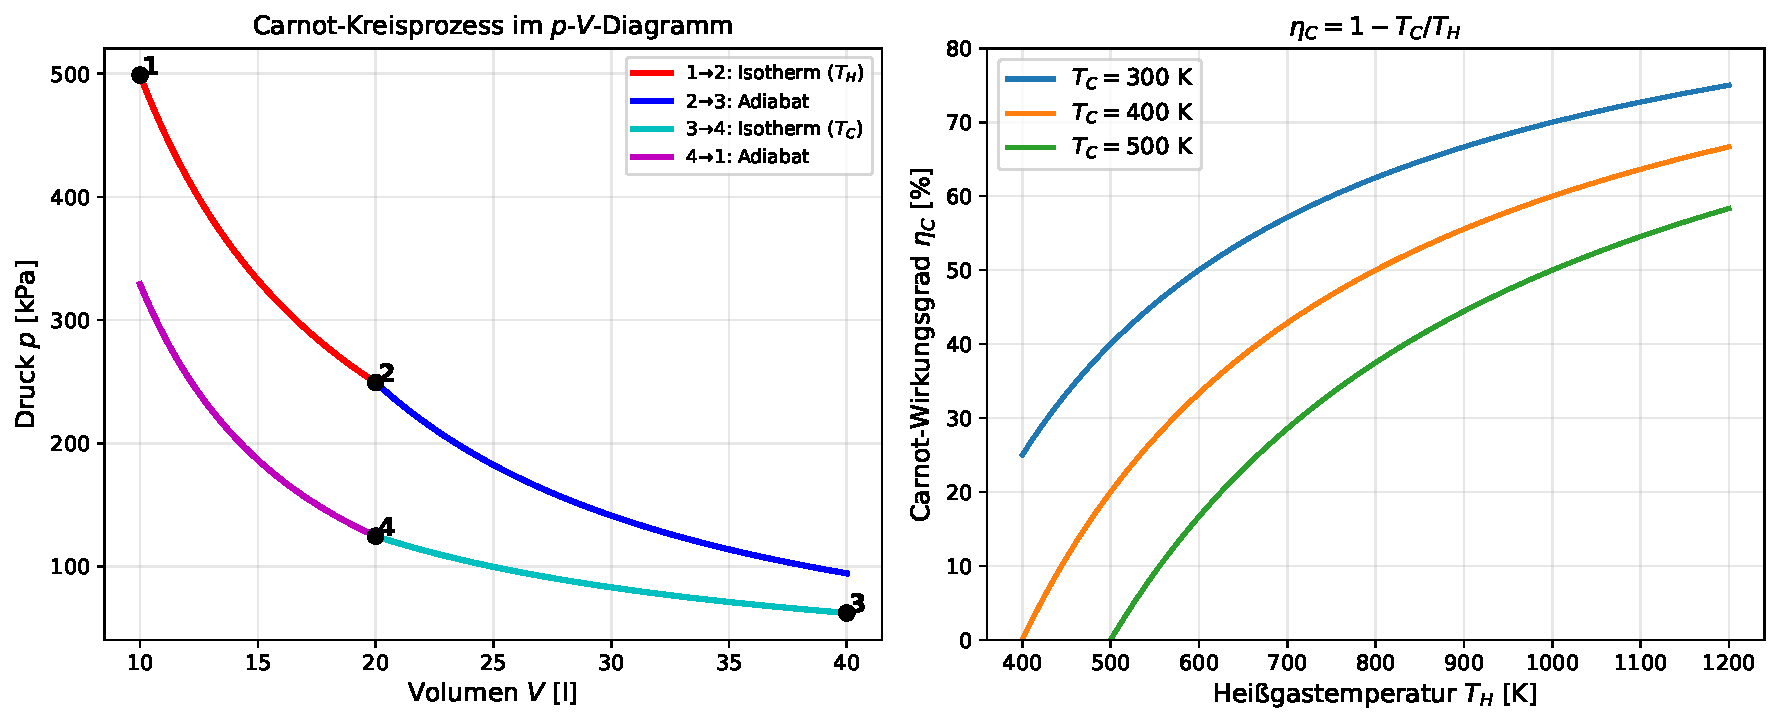
\includegraphics[width=0.92\textwidth]{plot_thermodynamik.pdf}
\caption{Links: Carnot-Kreisprozess im $p$-$V$-Diagramm mit zwei isothermen
($T_H$, $T_C$) und zwei adiabaten Zustands\"anderungen.
Rechts: Carnot-Wirkungsgrad $\eta_C = 1 - T_C/T_H$ als Funktion der
Heiztemperatur $T_H$ f\"ur verschiedene K\"uhltemperaturen $T_C$ --
mit steigendem $T_H$ oder sinkendem $T_C$ steigt $\eta_C$.}
\label{fig:thermo}
\end{figure}

\section{Zustandsgr\"o\ss{}en realer und idealer Gase}

\begin{definition}[Ideales Gasgesetz]
F\"ur ein \textbf{ideales Gas} (vernachl\"assigbare Molek\"ulvolumina und
-wechselwirkungen) gilt die \textbf{Zustandsgleichung}:
\[
  p\,V = n\,R\,T, \qquad p\,v = R_s\,T,
\]
mit universeller Gaskonstante $R = 8{,}314\,\mathrm{J/(mol\,K)}$,
spezifischem Volumen $v = V/m$ und spezifischer Gaskonstante
$R_s = R/M$ ($M$: molare Masse). F\"ur Luft: $R_s = 287\,\mathrm{J/(kg\,K)}$.
\end{definition}

\begin{definition}[Spezifische W\"armekapazit\"aten und Isentropenexponent]
Die spezifische W\"arme bei konstantem Volumen $c_v$ und konstantem Druck $c_p$:
\[
  c_p - c_v = R_s \quad (\text{Mayer-Gleichung f\"ur ideale Gase}).
\]
Der \textbf{Isentropenexponent}:
\[
  \kappa = \frac{c_p}{c_v} > 1 \quad (\text{Luft: } \kappa \approx 1{,}4).
\]
\end{definition}

\begin{satz}[Isentrope Zustands\"anderung]
F\"ur eine adiabate, reibungsfreie (isentrope) Zustands\"anderung gilt:
\[
  p\,V^\kappa = \mathrm{const}, \qquad \frac{T_2}{T_1} = \left(\frac{p_2}{p_1}\right)^{(\kappa-1)/\kappa}.
\]
\end{satz}
\begin{proof}
F\"ur adiabate Prozesse ($\delta Q = 0$): erster Hauptsatz ergibt
$\mathrm{d}U = -\delta W = -p\,\mathrm{d}V$, also $c_v\,\mathrm{d}T = -p\,\mathrm{d}v$.
Aus $pv = R_sT$: $p\,\mathrm{d}v + v\,\mathrm{d}p = R_s\,\mathrm{d}T$.
Einsetzen und mit $c_v$ dividieren: $\mathrm{d}p/p + \kappa\,\mathrm{d}v/v = 0$.
Integration: $\ln p + \kappa\ln v = \mathrm{const}$, also $p v^\kappa = \mathrm{const}$.
\end{proof}

\section{Technisch wichtige Kreisprozesse}

\begin{definition}[Otto-Kreisprozess]
Der \textbf{ideale Otto-Kreisprozess} (Modell f\"ur den Ottomotor) besteht aus:
isochorer W\"armezufuhr ($Q_1$, bei $V = \mathrm{const}$),
isentroper Expansion,
isochorer W\"armeabfuhr ($Q_2$),
isentroper Kompression.
Thermischer Wirkungsgrad:
\[
  \eta_{th,\text{Otto}} = 1 - \frac{1}{\varepsilon^{\kappa-1}},
\]
mit dem \textbf{Verdichtungsverh\"altnis} $\varepsilon = V_{\max}/V_{\min}$.
\end{definition}

\begin{beispiel}[Otto-Motor mit $\varepsilon = 10$]
F\"ur $\varepsilon = 10$, $\kappa = 1{,}4$:
\[
  \eta_{th} = 1 - \frac{1}{10^{0{,}4}} = 1 - \frac{1}{2{,}512} \approx 60{,}2\,\%.
\]
Reale Ottomotoren erreichen wegen Wandw\"armeverlusten, Restgas und
unvollst\"andiger Verbrennung nur $\eta \approx 30\ldots40\,\%$.
\end{beispiel}

\begin{definition}[Diesel-Kreisprozess]
Der \textbf{ideale Diesel-Kreisprozess} unterscheidet sich vom Otto-Prozess
durch isobare (statt isochore) W\"armezufuhr:
\[
  \eta_{th,\text{Diesel}} = 1 - \frac{1}{\varepsilon^{\kappa-1}}\cdot\frac{\phi^\kappa - 1}{\kappa(\phi-1)},
\]
mit dem \textbf{Einspritzverh\"altnis} $\phi = V_3/V_2$ (isobare Expansion bis $V_3$).
F\"ur $\phi = 1$ geht der Diesel-Prozess in den Otto-Prozess \"uber.
\end{definition}

\begin{definition}[Rankine-Kreisprozess -- Dampfturbine]
Der \textbf{Rankine-Prozess} ist das Modell f\"ur Dampfkraftwerke:
Pumpe (isentrope Druckerh\"ohung), Kessel (isobare W\"armezufuhr,
Dampferzeugung, \"Uberhitzung), Turbine (isentrope Expansion), Kondensator (isobare W\"armeabfuhr).
Thermischer Wirkungsgrad (vereinfacht):
\[
  \eta_{th} = \frac{W_T - W_P}{Q_1} \approx \frac{h_3 - h_4}{h_3 - h_1},
\]
mit den spezifischen Enthalpien $h_i$ an den Kreislaufpunkten.
Moderne Dampfkraftwerke erreichen $\eta \approx 45\ldots48\,\%$ (\"Uberkritisch).
\end{definition}

\section{W\"arme\"ubertragung}

\begin{definition}[W\"arme\"ubertragungsmechanismen]
Es gibt drei grunds\"atzliche Mechanismen:
\begin{itemize}
    \item[-] \textbf{W\"armeleitung} (Konduktion): $\dot{Q} = -\lambda A\dfrac{\mathrm{d}T}{\mathrm{d}x}$ (Fourier)
    \item[-] \textbf{W\"arme\"ubertragung} (Konvektion): $\dot{Q} = \alpha A (T_W - T_\infty)$ (Newton'sches Abk\"uhlungsgesetz)
    \item[-] \textbf{W\"armestrahlung}: $\dot{Q} = \varepsilon\sigma A T^4$ (Stefan-Boltzmann,
          $\sigma = 5{,}67\cdot10^{-8}\,\mathrm{W/(m^2 K^4)}$)
\end{itemize}
\end{definition}

\begin{satz}[W\"armedurchgang durch eine Wand]
F\"ur eine ebene Wand (Dicke $d$, W\"armenleitzahl $\lambda$) mit
Konvektion auf beiden Seiten ($\alpha_1$, $\alpha_2$) gilt der
W\"armedurchgangskoeffizient:
\[
  k = \frac{1}{\dfrac{1}{\alpha_1} + \dfrac{d}{\lambda} + \dfrac{1}{\alpha_2}},
  \qquad \dot{Q} = k\,A\,(T_1 - T_2).
\]
\end{satz}
\begin{proof}
Die einzelnen thermischen Widerst\"ande ($R_1 = 1/\alpha_1 A$,
$R_2 = d/\lambda A$, $R_3 = 1/\alpha_2 A$) schalten sich in Reihe
(analogie zur elektrischen Reihenschaltung von Widerst\"anden):
$R_{ges} = R_1 + R_2 + R_3 = (1/\alpha_1 + d/\lambda + 1/\alpha_2)/A = 1/(kA)$.
\end{proof}

% ============================================================

% ====== Erweiterung Wärmeübertragung ======

\section{Wärmeübertrager und Kältemaschinen}

\begin{definition}[Wärmeübertrager -- Typen und Berechnung]
\textbf{Wärmeübertrager} übertragen Wärme zwischen zwei Fluidströmen.
Wichtige Bauformen:
\begin{itemize}
    \item[-] \textbf{Gleichstrom}: beide Fluide strömen in gleicher Richtung;
          Austrittstemperaturdifferenz limitiert
    \item[-] \textbf{Gegenstrom}: maximaler Wärmeübertrag; Austrittstemperatur
          kann Eintrittstemperatur des Gegenstroms überschreiten
    \item[-] \textbf{Kreuzstrom}: senkrechte Strömungen; Plattenwärmeübertrager
    \item[-] \textbf{Manteldurchströmter Rohrbündelwärmetauscher}:
          Rohre in Mantel; chemische Industrie
\end{itemize}
Die übertragene Wärmeleistung:
\[
  \dot{Q} = k\,A\,\Delta T_{lm}, \qquad
  \Delta T_{lm} = \frac{\Delta T_1 - \Delta T_2}{\ln(\Delta T_1/\Delta T_2)}
\]
(\textbf{logarithmische mittlere Temperaturdifferenz} $\Delta T_{lm}$
für Gleich- und Gegenstrom).
\end{definition}

\begin{satz}[Kälteleistungszahl (COP) einer Kältemaschine]
Eine Kältemaschine entzieht der Kältequelle (Temperatur $T_C$) die
Wärme $|Q_C|$ durch Zufuhr von Arbeit $W$.
Die \textbf{Leistungszahl}:
\[
  \varepsilon = \frac{|Q_C|}{W} = \frac{T_C}{T_H - T_C} \quad (\text{Carnot-Kältemaschine}).
\]
Reale Kältemaschinen (Kompressionskältemaschinen) erreichen
$\varepsilon = 2\ldots5$ (typische Klimaanlage).
\end{satz}
\begin{proof}
Für die Carnot-Kältemaschine gilt energetisch: $W = Q_H - |Q_C|$
und thermisch: $|Q_C|/T_C = Q_H/T_H$ (reversibel).
Daher $\varepsilon = |Q_C|/(Q_H - |Q_C|) = T_C/(T_H - T_C)$.
\end{proof}

\begin{beispiel}[Haushalts-Kühlschrank]
Ein Kühlschrank ($T_C = 5^\circ\mathrm{C} = 278\,\mathrm{K}$,
$T_H = 35^\circ\mathrm{C} = 308\,\mathrm{K}$, Carnot-COP):
\[
  \varepsilon_C = \frac{278}{308 - 278} = \frac{278}{30} \approx 9{,}3.
\]
Mit $\varepsilon_{\text{real}} \approx 3$ und $\dot{Q}_C = 100\,\mathrm{W}$ (Kühlleistung):
Elektrische Leistungsaufnahme $P = \dot{Q}_C/\varepsilon_{\text{real}} \approx 33\,\mathrm{W}$.
\end{beispiel}

% ====== Erweiterung Strömungslehre: Turbulenz ======

\section{Grenzschicht und Turbulenz}

\begin{definition}[Grenzschichttheorie nach Prandtl]
In der \textbf{Prandtl'schen Grenzschicht} nahe einer überströmten
Wand vernachlässigt man den Druck quer zur Wand und vereinfacht
die Navier-Stokes-Gleichungen. Für die laminare Grenzschichtdicke
$\delta$ auf einer überströmten Platte (Länge $x$, Anströmgeschwindigkeit $v_\infty$):
\[
  \delta(x) = 5{,}0\,\sqrt{\frac{\nu x}{v_\infty}} = \frac{5{,}0\,x}{\sqrt{Re_x}},
  \qquad Re_x = \frac{v_\infty x}{\nu}.
\]
Der lokale Reibungsbeiwert:
\[
  c_f(x) = \frac{\tau_w}{\tfrac{1}{2}\rho v_\infty^2} = \frac{0{,}664}{\sqrt{Re_x}}.
\]
\end{definition}
\begin{proof}
Blasius (1908) löste die Grenzschichtgleichungen durch Ähnlichkeitslösung
(Strom\-funktion $\psi = \sqrt{v_\infty\nu x}\,f(\eta)$,
Ähnlichkeitsvariable $\eta = y\sqrt{v_\infty/(\nu x)}$).
Die numerische Lösung der resultierenden Blasius-DGL
$f''' + ff''/2 = 0$ ergibt $f''(0) = 0{,}332$, woraus der Reibungsbeiwert folgt.
\end{proof}

\begin{beobachtung}[Turbulente Grenzschicht und logarithmisches Wandgesetz]
In der \textbf{turbulenten Grenzschicht} gilt das \textbf{logarithmische Wandgesetz}:
\[
  u^+ = \frac{1}{\kappa}\ln(y^+) + B,
  \qquad u^+ = \frac{u}{u_\tau}, \quad y^+ = \frac{y\,u_\tau}{\nu},
  \quad u_\tau = \sqrt{\tau_w/\rho},
\]
mit von-Kármán-Konstante $\kappa \approx 0{,}41$ und $B \approx 5{,}0$.
Dieses Gesetz gilt für $30 \lesssim y^+ \lesssim 300$ (logarithmische Schicht).
Wandnächster Bereich ($y^+ < 5$): viskose Unterschicht $u^+ = y^+$.
\end{beobachtung}

% ====== Fertigungstechnik Erweiterung ======

\section{Schweißtechnik und Fügetechnologie}

\begin{definition}[Schweißverfahren nach DIN 1910]
Schweißen ist das Verbinden von Werkstoffen durch \emph{Wärme}
und/oder \emph{Druck}, mit oder ohne Zusatzwerkstoff.
Wichtige thermische Schweißverfahren:
\begin{itemize}
    \item[-] \textbf{MSG-Schweißen} (MIG/MAG, DIN EN ISO 14341):
          Metall-Schutzgas-Schweißen; häufigste Verfahren für Stahl;
          abschmelzende Elektrode; Schutzgas CO$_2$/Ar-Gemisch (MAG) oder Ar (MIG)
    \item[-] \textbf{WIG-Schweißen} (TIG, DIN EN ISO 636):
          Wolfram-Inertgas; nicht abschmelzende W-Elektrode; Ar-Schutzgas;
          höchste Nahtqualität; Edelstahl, Al, Ti
    \item[-] \textbf{Laserstrahlschweißen} (DIN EN ISO 11553):
          Hochenergiedichtestrahl; Tiefschweißen (Keyhole); Automotive-Karosserie
    \item[-] \textbf{Elektronenstrahlschweißen}: im Vakuum; tiefste Einbrandtiefe ($> 100\,\mathrm{mm}$)
    \item[-] \textbf{Reibrührschweißen (FSW)}: Festphasen-Verbindung;
          Aluminium; keine Heißrisse; Luft- und Raumfahrt
\end{itemize}
\end{definition}

\begin{satz}[Wärmeeintrag und Abkühlgeschwindigkeit beim Schweißen]
Der \textbf{Streckenenergie} (Wärmeeintrag pro Länge) beim Schweißen:
\[
  Q_s = \eta\,\frac{U\,I}{v_s} \quad [\mathrm{J/mm}],
\]
mit thermischem Wirkungsgrad $\eta$ (MIG: $\eta \approx 0{,}8$;
Laser: $\eta \approx 0{,}4$), Lichtbogenspannung $U$, Schweißstrom $I$
und Schweißgeschwindigkeit $v_s$.
Die Abkühlgeschwindigkeit $t_{8/5}$ (Zeit von $800$ auf $500^\circ\mathrm{C}$)
bestimmt das Nahtgefüge:
\[
  t_{8/5} \approx \frac{4300 - 4{,}3\,T_0}{(T_0 - 100)^2}\cdot Q_s^2
  \quad (\text{3D-Wärmeleitung, dicke Bleche}),
\]
mit Vorwärmtemperatur $T_0$. Langsame Abkühlung (großes $t_{8/5}$) ergibt
Ferrit/Bainit (zäh); schnelle Abkühlung Martensit (hart, aber spröde).
\end{satz}


% ====== Letzte Erweiterung: dichte Inhaltsblöcke in bestehende Kapitel ======

\section{Thermodynamik technischer Gase und Verbrennungsprozesse}

\begin{definition}[Reales Gas -- van-der-Waals-Gleichung]
Das ideale Gasgesetz versagt bei hohen Drücken und tiefen Temperaturen.
Die \textbf{van-der-Waals-Gleichung} korrigiert für Molekülvolumen $b$
und intermolekulare Anziehungskräfte $a$:
\[
  \left(p + \frac{a}{v^2}\right)(v - b) = R_s T.
\]
Bei hohem Druck ($v \to b$): Druck steigt stark an (Abstoßung).
Bei tiefem $T$: Verflüssigung durch Anziehungskräfte ($a/v^2$-Term dominant).
Der kritische Punkt: $p_c = a/(27b^2)$, $v_c = 3b$, $T_c = 8a/(27R_s b)$.
\end{definition}

\begin{definition}[Verbrennung -- Stöchiometrie und Luftzahl]
Vollständige Verbrennung von Methan (Erdgas):
\[
  \mathrm{CH_4 + 2O_2 \to CO_2 + 2H_2O}, \qquad
  \Delta H_u = -802\,\mathrm{kJ/mol}.
\]
Theoretischer Sauerstoffbedarf $L_{min}$ und Luftbedarf $L_{0}$
(Luft: 21\,\% O$_2$, Molmasse 29\,g/mol).
Die \textbf{Luftzahl} $\lambda = L/L_{0}$:
\begin{itemize}
    \item[-] $\lambda < 1$: fettes Gemisch (Luftmangel); unvollständige Verbrennung; CO-Emission
    \item[-] $\lambda = 1$: stöchiometrisches Gemisch; höchste Flammentemperatur
    \item[-] $\lambda > 1$: mageres Gemisch (Luftüberschuss); niedrigere Temperatur; niedrigere NO$_x$
\end{itemize}
\end{definition}

\begin{beispiel}[Flammentemperatur bei $\lambda = 1$]
Vereinfachte adiabate Flammentemperatur für Methan/Luft ($\lambda = 1$):
\[
  T_{ad} = T_0 + \frac{\Delta H_u}{(m_{CH_4} + m_{Luft})\,c_p^{ges}}
  \approx 298 + \frac{802000}{(16 + 2\cdot32/0{,}21)\cdot10^{-3}\cdot1100}
  \approx 2230\,\mathrm{K}.
\]
Reale Flammentemperaturen liegen durch Dissoziation der Verbrennungsprodukte
bei $\approx 2000\,\mathrm{K}$ (CO$_2$, H$_2$O dissoziieren bei hohen Temperaturen).
\end{beispiel}

\section{Akustik und Lärmschutz im Maschinenbau}

\begin{definition}[Schalldruckpegel und Schallleistungspegel]
Schall ist eine mechanische Druckwelle. Der \textbf{Schalldruckpegel}:
\[
  L_p = 20\log_{10}\frac{p}{p_0}\,[\mathrm{dB}], \quad p_0 = 20\,\mu\mathrm{Pa}
  \;(\text{Hörschwelle}).
\]
Der \textbf{Schallleistungspegel}:
\[
  L_W = 10\log_{10}\frac{P}{P_0}\,[\mathrm{dB}], \quad P_0 = 10^{-12}\,\mathrm{W}.
\]
Schallausbreitung im Freifeld: $L_p = L_W - 20\log_{10}r - 11\,\mathrm{dB}$
(Abstandsgesetz; Pegelabnahme $6\,\mathrm{dB}$ je Entfernungsverdoppelung).
\end{definition}

\begin{satz}[Wellengleichung und akustische Moden]
Die Schallausbreitung in einem idealen Medium (homogen, ruhend, ohne Viskosität)
gehorcht der \textbf{Wellengleichung}:
\[
  \frac{\partial^2 p}{\partial t^2} = c^2\,\nabla^2 p,
  \qquad c = \sqrt{\kappa R_s T} \quad (\text{Schallgeschwindigkeit im Gas}).
\]
Für Luft bei $T = 293\,\mathrm{K}$: $c = \sqrt{1{,}4\cdot287\cdot293} \approx 343\,\mathrm{m/s}$.
\end{satz}
\begin{proof}
Aus der Linearisierung der Euler-Gleichungen (Kontinuität + Impuls)
für kleine Störungen $p = p_0 + p'$, $\rho = \rho_0 + \rho'$, $\vec{v} = \vec{v}'$
folgt die Wellengleichung. Die Schallgeschwindigkeit ergibt sich aus der
isentropen Zustandsänderung: $(\partial p/\partial \rho)_s = \kappa p_0/\rho_0 = c^2$.
\end{proof}

\begin{beobachtung}[Körperschall und Körperschalldämmung]
\textbf{Körperschall} entsteht durch Schwingungsübertragung von Maschinen
auf umgebende Strukturen und wird dort in Luftschall (Abstrahlung) umgewandelt.
Maßnahmen zur Körperschalldämmung:
\begin{itemize}
    \item[-] \textbf{Elastische Lagerung}: Maschine auf Federn/Elastomeren;
          Einfügungsdämmmaß $D_E = 20\log_{10}(\eta/\sqrt{(\eta^2-1)})$ (für $\eta > \sqrt{2}$)
    \item[-] \textbf{Tilger und Dämpfer}: aktive oder passive Schwingungsminderung
          an der Quelle (tuned vibration absorber)
    \item[-] \textbf{Schwere Massen (Fundamente)}: Masse erhöht Impedanz;
          $f_0 = (1/2\pi)\sqrt{c_{Unterbau}/m_{Fundament}}$ tief halten
    \item[-] \textbf{Körperschallisolation}: Unterbrechung von Schallpfaden
          durch weiche Zwischenlagen (Gleitlager, Manschetten)
\end{itemize}
\end{beobachtung}

\section{Additive Fertigung -- Prozessphysik und Qualitätssicherung}

\begin{beobachtung}[Physik des Laser-Pulverbettschmelzens (LPBF/SLM)]
Beim Laser-Pulverbettschmelzen entstehen komplexe Wechselwirkungen:
\begin{itemize}
    \item[-] \textbf{Absorptionsgrad}: Laserenergie wird an der Pulveroberfläche
          absorbiert; Tiefschweißen (Keyhole-Modus) bei hoher Intensität ($> 10^6\,\mathrm{W/cm^2}$)
    \item[-] \textbf{Schmelzbadströmung}: Marangoni-Konvektion (thermische Oberflächenspannung),
          Dampfreaktionskraft, Kapillarkraft bestimmen die Schmelzbadform
    \item[-] \textbf{Eigenspannungen}: Schnelle Abkühlung erzeugt hohe Zugeigenspannungen
          ($\approx 0{,}5\,R_e$) -- Wärmenachbehandlung oder Stützstrukturen nötig
    \item[-] \textbf{Porosität}: Keyhole-Poren (Gasblasen), Lack-of-Fusion-Poren
          (unaufgeschmolzenes Pulver) -- durch Prozessparameteroptimierung ($E_v = P/(v\cdot h\cdot d)$,
          volumetrische Energiedichte) minimierbar
    \item[-] \textbf{In-situ Qualitätsüberwachung}: Melt-Pool-Monitoring,
          Thermal Imaging, optische Tomographie im Bauvorgang
\end{itemize}
\end{beobachtung}

\section{Hochtemperaturwerkstoffe und thermische Barriereschichten}

\begin{definition}[Kriechverhalten von Hochtemperaturwerkstoffen]
Oberhalb von $\approx 0{,}4\,T_{Schmelz}$ verformen sich Metalle unter
dauerhafter Last zeitabhängig: \textbf{Kriechen}.
Das Norton-Kriechgesetz:
\[
  \dot{\varepsilon}_{cr} = A\,\sigma^n\,e^{-Q/(RT)},
\]
mit materialabhängigem Kriechexponent $n$ (Metalle: $n \approx 3\ldots8$),
Aktivierungsenergie $Q$, universeller Gaskonstante $R$ und Temperatur $T$.
\end{definition}

\begin{beobachtung}[Thermische Barriereschichten in Gasturbinen]
Gasturbinenschaufeln moderner Triebwerke (Heißgastemperatur $> 1700^\circ\mathrm{C}$,
Schaufelmaterial-Schmelzpunkt $\approx 1350^\circ\mathrm{C}$) werden durch
\textbf{Thermal Barrier Coatings} (TBC) geschützt:
\begin{itemize}
    \item[-] \textbf{Topschicht}: 7YSZ (zirconia stabilisiert mit 7\,\% Yttria);
          Wärmeleitfähigkeit $\lambda \approx 2\,\mathrm{W/(mK)}$; Schichtdicke $\approx 100\ldots300\,\mu\mathrm{m}$
    \item[-] \textbf{Haftvermittler}: MCrAlY (M = Ni, Co); Oxidationsschutz;
          bildet schützende $\alpha$-Al$_2$O$_3$-Schicht (TGO, Thermally Grown Oxide)
    \item[-] \textbf{Innenkühlung}: Serpentinenkanäle + Filmkühlung durch
          Bohrungen; Kühlluft $\approx 600^\circ\mathrm{C}$;
          Wärmeübergangskoeffizient innen $\alpha \approx 1000\ldots5000\,\mathrm{W/(m^2 K)}$
\end{itemize}
Das TBC-System ermöglicht $\Delta T \approx 100\ldots200\,\mathrm{K}$ Temperaturgradient --
dies steigert den Turbinenwirkungsgrad erheblich (jeder K Temperaturerhöhung
$\approx 0{,}3\,\%$ Wirkungsgradgewinn).
\end{beobachtung}

\chapter{Werkstofftechnik}
% ============================================================

Werkstofftechnik umfasst Auswahl, Charakterisierung, Verarbeitung
und Einsatzgrenzen technischer Werkstoffe. Die richtige Werkstoffwahl
ist oft entscheidend f\"ur Sicherheit, Lebensdauer, Wirtschaftlichkeit
und Nachhaltigkeit eines Maschinenbausystems.

\section{Aufbau und Eigenschaften metallischer Werkstoffe}

\begin{definition}[Kristallstruktur der Metalle]
Metalle ordnen sich in regelm\"a\ss{}igen \textbf{Kristallgittern}.
Die h\"aufigsten Gittertypen:
\begin{itemize}
    \item[-] \textbf{Kubisch-raumzentriert (krz)}: Eisen ($\alpha$-Fe, $\delta$-Fe),
          Chrom, Wolfram, Molybd\"an; Koordinationszahl 8
    \item[-] \textbf{Kubisch-fl\"achenzentriert (kfz)}: Eisen ($\gamma$-Fe), Aluminium,
          Kupfer, Nickel; Koordinationszahl 12; Packungsdichte $74\,\%$
    \item[-] \textbf{Hexagonal dichtgepackt (hdp)}: Magnesium, Titan, Zink,
          Kobalt; Packungsdichte $74\,\%$
\end{itemize}
Plastische Verformbarkeit h\"angt vom Gleitsystem ab: kfz-Metalle
(12 Gleitsysteme) sind gut formbar; hdp-Metalle (nur wenige Gleitsysteme)
sind spröder.
\end{definition}

\begin{satz}[Phasenregel von Gibbs]
In einem thermodynamischen System mit $K$ Komponenten, $P$ Phasen und
dem Freiheitsgrad $F$ (Anzahl unabh\"angig ver\"anderlicher Zustandsgr\"o\ss{}en) gilt:
\[
  F = K - P + 2 \quad (\text{allgemein}), \qquad F = K - P + 1 \quad (\text{isobar}).
\]
\end{satz}
\begin{proof}
Im Gleichgewicht m\"ussen f\"ur jede Komponente $k$ die chemischen Potentiale
$\mu_k^{(1)} = \mu_k^{(2)} = \cdots = \mu_k^{(P)}$ in allen $P$ Phasen gleich sein.
Das ergibt $K(P-1)$ Bedingungen an die $K(P-1)+2$ Freiheitsgrade
(Konzentration jeder Komponente in jeder Phase plus $T$ und $p$).
Differenz: $F = K(P-1)+2 - K(P-1) = K - P + 2$.
\end{proof}

\begin{figure}[htbp]
\centering
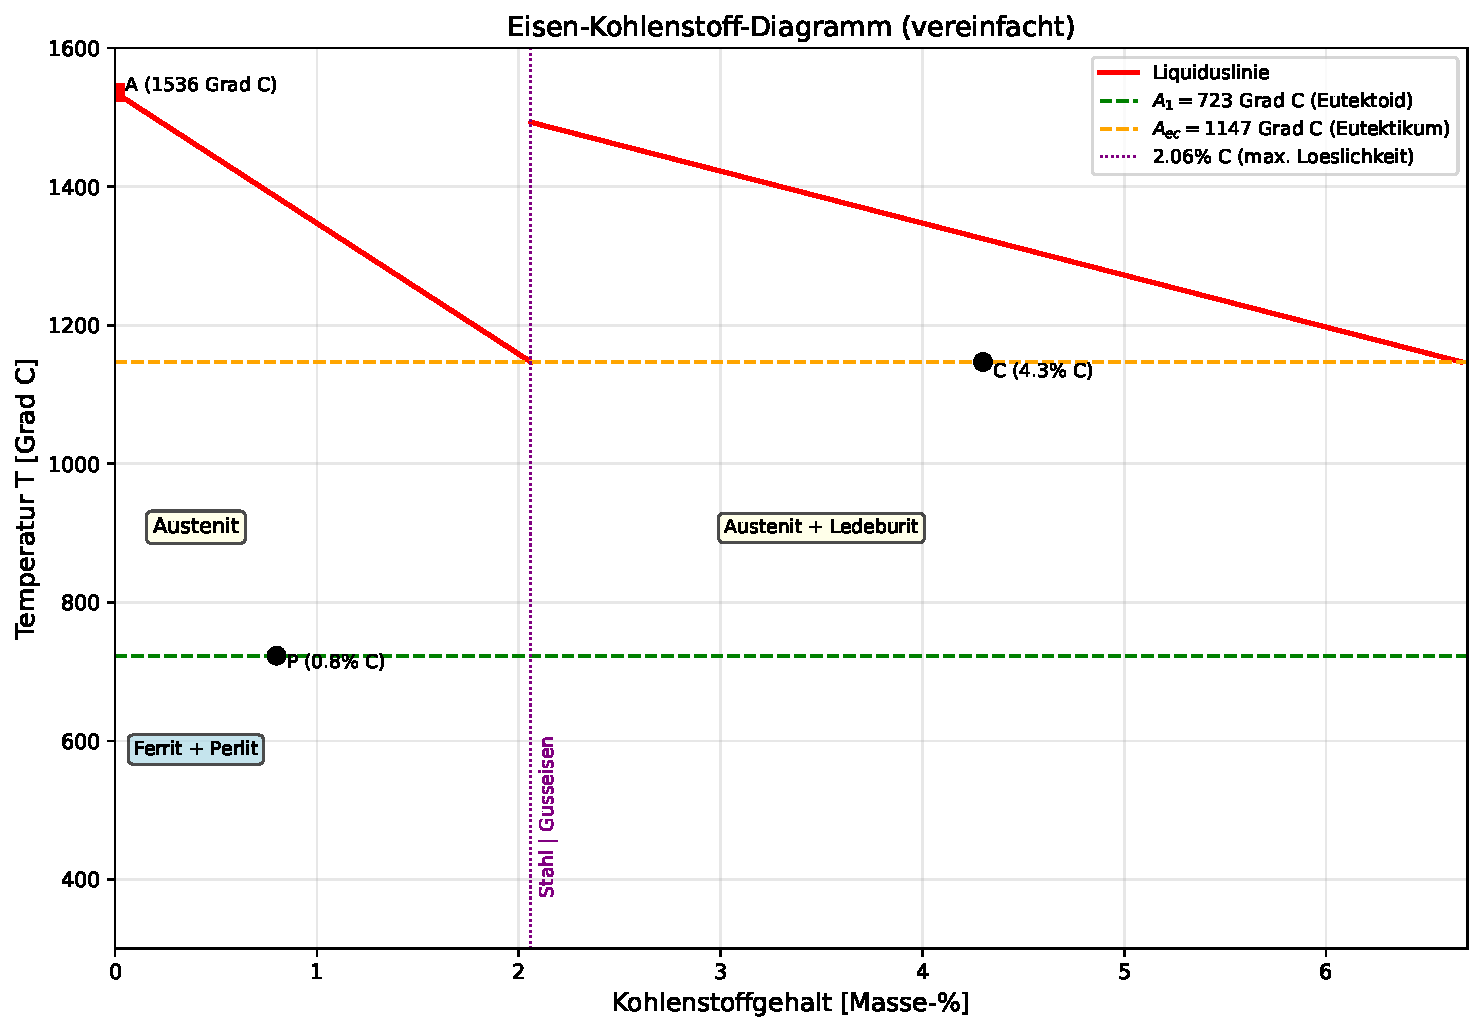
\includegraphics[width=0.78\textwidth]{plot_eisen_kohlenstoff.pdf}
\caption{Eisen-Kohlenstoff-Diagramm (vereinfacht): Die Liquiduslinie begrenzt
den Erstarrungsbereich. Bei 0{,}8\,\% C und $723^\circ\mathrm{C}$ (Punkt P)
bildet sich durch den eutektoiden Zerfall des Austenits Perlit
(Ferrit-Zementit-Lamellengemisch). Stähle (links der 2{,}06\,\%-Grenze)
und Gusseisen (rechts) unterscheiden sich grundlegend in Verarbeitbarkeit.}
\label{fig:eisen}
\end{figure}

\section{Eisenwerkstoffe}

\begin{definition}[Stahl -- Klassifikation nach DIN EN 10020]
\textbf{Stahl} ist Eisen mit $w_C < 2{,}06\,\%$ (Massenanteil Kohlenstoff):
\begin{itemize}
    \item[-] \textbf{Unlegierter Stahl}: ohne Mindestgehalte an Legierungselementen;
          Beispiel: S235 (Streckgrenze $R_e \ge 235\,\mathrm{MPa}$), S355 (Hochfester Baustahl)
    \item[-] \textbf{Niedriglegierter Stahl}: Summe der Legierungsgehalte $< 5\,\%$;
          z.\,B.\ 42CrMo4 (Verg\"utungsstahl f\"ur Wellen und Zahnr\"ader)
    \item[-] \textbf{Hochlegierter Stahl}: mind. ein Element $\ge 5\,\%$;
          z.\,B.\ 1.4301 (X5CrNi18-10, nichtrostend)
    \item[-] \textbf{Werkzeugstahl}: hohe H\"arte, Verschlei\ss{}best\"andigkeit
\end{itemize}
\end{definition}

\begin{satz}[Martensitbildung und H\"artung]
Wird Austenitit schnell auf Temperaturen unterhalb der Martensit-Starttemperatur
$M_s$ abgekuehlt (Abschrecken), bildet sich \textbf{Martensit}:
ein tetragonal verzerrtes, supersaturiertes Eisengitter mit
erzwungenem Kohlenstoffgehalt. Die H\"arte steigt mit dem Kohlenstoffgehalt
steil an ($> 60\,\mathrm{HRC}$ f\"ur $w_C > 0{,}6\,\%$).
Die Martensit-Starttemperatur (empirisch):
\[
  M_s \approx 539 - 423\,w_C - 30\,w_{Mn} - 18\,w_{Ni} - 12\,w_{Cr} - 7\,w_{Mo}\;[^\circ\mathrm{C}].
\]
\end{satz}

\begin{definition}[W\"armebehandlungsverfahren]
Wichtige Verfahren zur gezielten Eigenschafts\"anderung:
\begin{itemize}
    \item[-] \textbf{Gluhen} (Normalgl\"uhen, Weichgl\"uhen, Spannungsarmgl\"uhen):
          Eigenspannungsabbau, Rekristallisation, Gef\"ugehomogenisierung
    \item[-] \textbf{H\"arten und Anlassen} (Verg\"uten): Martensitbildung + Anlassen
          bei $150\ldots600^\circ\mathrm{C}$ ergibt Verg\"utungsgef\"uge
          mit hoher Z\"ahigkeit und Festigkeit
    \item[-] \textbf{Randschichtverfahren}: Ind\"uktionsh\"arten, Einsatzh\"arten
          (Aufkohlen), Nitrieren -- nur Randschicht wird geh\"artet;
          der Z\"ahe Kern bleibt erhalten
    \item[-] \textbf{Thermomechanische Behandlung}: Kombination aus Umformung
          und W\"armebehandlung f\"ur HSLA-St\"ahle im Fahrzeugbau
\end{itemize}
\end{definition}

\section{Nichteisenmetalle}

\begin{definition}[Aluminium und Aluminiumlegierungen]
Aluminium ($\rho = 2700\,\mathrm{kg/m^3}$, $E = 70\,\mathrm{GPa}$) bietet
eine einzigartige Kombination aus Leichtigkeit, Korrosionsbest\"andigkeit
und Formbarkeit.
\begin{itemize}
    \item[-] \textbf{Knetlegierungen} (EN AW-...): Al-Mg (5xxx), Al-Mg-Si (6xxx),
          Al-Zn-Mg-Cu (7xxx -- h\"ochste Festigkeiten im Flugzeugbau: $R_m > 550\,\mathrm{MPa}$)
    \item[-] \textbf{Gusslegierungen} (EN AC-...): Al-Si (F\"uleggierung, $T\approx600^\circ\mathrm{C}$)
    \item[-] \textbf{Ausscheidungsh\"artung}: durch Ausl\"agern (Glühen, Abschrecken,
          Auslagern bei $T\approx 120\ldots180^\circ\mathrm{C}$) bilden sich
          feine Ausscheidungen, die Versetzungsbewegung behindern
\end{itemize}
\end{definition}

\begin{definition}[Kupfer, Titan und weitere NE-Metalle]
\begin{itemize}
    \item[-] \textbf{Kupfer} ($\rho = 8900\,\mathrm{kg/m^3}$, $E = 120\,\mathrm{GPa}$):
          excellente elektrische Leitf\"ahigkeit; Bronze (Cu-Sn), Messing (Cu-Zn)
    \item[-] \textbf{Titan} ($\rho = 4500\,\mathrm{kg/m^3}$, $E = 115\,\mathrm{GPa}$):
          h\"ochste spezifische Festigkeit, hervorragende Korrosionsbest\"andigkeit;
          Luft- und Raumfahrt, Medizintechnik
    \item[-] \textbf{Magnesium} ($\rho = 1740\,\mathrm{kg/m^3}$): leichtestes
          konstruktiv einsetzbares Metall; Lenkgeh\"ause, Geh\"ause im Fahrzeugbau
    \item[-] \textbf{Nickel-Superlegierungen}: Betrieb bis $\approx 1100^\circ\mathrm{C}$;
          Turbinenschaufeln in Fluggasturbinen
\end{itemize}
\end{definition}

\section{Polymere und Verbundwerkstoffe}

\begin{definition}[Kunststoffklassen]
\begin{itemize}
    \item[-] \textbf{Thermoplaste}: erweichen reversibel beim Erw\"armen (Schmelzen);
          recyclef\"ahig; z.\,B.\ Polyethylen (PE), Polyamid (PA), Polycarbonat (PC)
    \item[-] \textbf{Duroplaste}: vernetzen irreversibel beim Aush\"arten;
          hohe H\"arte, aber spr\"ode; z.\,B.\ Epoxidharz (EP), Phenolharz
    \item[-] \textbf{Elastomere}: weitmaschig vernetzt; hochelastische Verformung;
          z.\,B.\ Naturkautschuk, EPDM (Dichtungen, Reifen)
\end{itemize}
\end{definition}

\begin{definition}[Faserverb\"undwerkstoffe]
\textbf{Faserverb\"undwerkstoffe} (FVW) kombinieren hochfeste Fasern
(Kohlenstoff, Glas, Aramid) in einer Kunststoffmatrix (meist EP-Harz).
Eigenschaften von CFK (Kohlenstofffaserverst\"arkter Kunststoff):
\begin{itemize}
    \item[-] Spezifische Zugfestigkeit: $\sim 1000\,\mathrm{MPa/(g/cm^3)}$ -- ca. $5\times$ Stahl
    \item[-] Spezifischer E-Modul: bis $250\,\mathrm{GPa/(g/cm^3)}$ (unidirektional) -- ca. $8\times$ Stahl
    \item[-] Anisotrop: Eigenschaften stark richtungsabh\"angig (Laminatdesign!)
    \item[-] Herausforderungen: aufw\"andige Fertigung, schlechte Recyclierbarkeit,
          Empfindlichkeit gegen Schlagbeanspruchung (BVID -- Barely Visible Impact Damage)
\end{itemize}
\end{definition}

\begin{satz}[Voigt-Reuss-Schranken -- E-Modul eines Verbundwerkstoffs]
F\"ur einen Verbundwerkstoff aus Faser (Volumenanteil $V_f$, E-Modul $E_f$)
und Matrix (Volumenanteil $V_m = 1-V_f$, E-Modul $E_m$) gelten:
\[
  E_{\|} = V_f E_f + V_m E_m \quad (\text{Voigt, Iso-Dehnungs-Modell, Faserrichtung}),
\]
\[
  E_{\perp} = \frac{E_f E_m}{V_f E_m + V_m E_f} \quad (\text{Reuss, senkrecht zur Faser}).
\]
\end{satz}
\begin{proof}
\textit{Voigt}: Bei gleicher Dehnung $\varepsilon$ in Faserrichtung
(beide Phasen werden gleich gedehnt) teilt sich die Kraft proportional
zu $E_f A_f$ und $E_m A_m$ auf. Der effektive E-Modul:
$E_{\|} = \sigma_{\text{ges}}/\varepsilon = (E_f V_f + E_m V_m)\sigma_0/\sigma_0 = V_f E_f + V_m E_m$.
\textit{Reuss}: Bei gleicher Spannung $\sigma$ (senkrecht zur Faser)
addieren sich die Dehnungen: $\varepsilon_{\text{ges}} = V_f\varepsilon_f + V_m\varepsilon_m
= \sigma(V_f/E_f + V_m/E_m)$, also $E_{\perp} = 1/(V_f/E_f + V_m/E_m)$.
\end{proof}

% ============================================================

\section{Gefüge, Wärmebehandlungsdiagramme und Eigenspannungen}

\begin{definition}[Zeit-Temperatur-Umwandlungsdiagramm (ZTU)]
Das \textbf{ZTU-Diagramm} (isothermes ZTU: isotherm abgekühlt; kontinuierliches ZTU: KU)
beschreibt die Umwandlung des Austenits beim Abkühlen von Stahl.
Im \textbf{kontinuierlichen ZTU-Diagramm} sind Abkühlkurven mit
den entstehenden Gefügephasen eingetragen:
\begin{itemize}
    \item[-] \textbf{Schnelle Abkühlung} (Abschrecken in Wasser/Öl): Martensit ($M_s$-Linie)
    \item[-] \textbf{Mittlere Abkühlung}: Bainit (oberer und unterer Bainit)
    \item[-] \textbf{Langsame Abkühlung} (Luftkühlung, Ofenkühlung): Ferrit + Perlit
\end{itemize}
Die kritische Abkühlgeschwindigkeit $v_{krit}$ trennt martensitische
von bainitischer/perlitischer Umwandlung. Für einen unlegierten C45-Stahl:
$v_{krit} \approx 200\,\mathrm{K/s}$; für legierten 42CrMo4:
$v_{krit} \approx 2\,\mathrm{K/s}$ (bessere Durchhärtbarkeit).
\end{definition}

\begin{beobachtung}[Eigenspannungen und Verzug beim Härten]
Beim Abschrecken entstehen \textbf{Eigenspannungen} aus zwei Quellen:
\begin{itemize}
    \item[-] \textbf{Thermische Eigenspannungen}: Außen kühlt schnell ab
          und zieht sich zusammen, während innen noch warm -- Druckeigenspannungen innen,
          Zugeigenspannungen außen (dann Umkehr beim weiteren Abkühlen)
    \item[-] \textbf{Umwandlungseigenspannungen}: Martensitumwandlung
          geht mit Volumenzunahme $(\approx 1\ldots4\,\%)$ einher;
          Randschicht wandelt zuerst um -- Druckeigenspannungen im Kern nach Umwandlung
\end{itemize}
Ergebnis: Gehärteter Stahl zeigt oft \emph{Druckeigenspannungen an der Oberfläche}
($-400$ bis $-800\,\mathrm{MPa}$) -- vorteilhaft für Ermüdungsfestigkeit.
Schleifbrand kann diese in Zugeigenspannungen umkehren -- gefährlich!
\end{beobachtung}

\section{Nichtlineare Mechanik und große Verformungen}

\begin{definition}[Geometrische Nichtlinearität]
Bei großen Verformungen versagt die lineare Theorie ($\varepsilon = \Delta l/l_0$).
Korrekte kinematische Maße:
\begin{itemize}
    \item[-] \textbf{Green-Lagrange-Verzerrungstensor}: $E_{ij} = \tfrac{1}{2}(F_{ki}F_{kj} - \delta_{ij})$,
          mit Deformationsgradient $F_{ij} = \partial x_i/\partial X_j$
          (aktuelle Koordinaten $x_i$, Referenzkoordinaten $X_j$)
    \item[-] \textbf{Almansi-Eulerscher Verzerrungstensor}: in aktueller Konfiguration
    \item[-] \textbf{Cauchy-Spannung} $\boldsymbol{\sigma}$: Kraft pro Fläche in aktueller Konfiguration
    \item[-] \textbf{2. Piola-Kirchhoff-Spannung} $\mathbf{S}$: in Referenzkonfiguration;
          konjugiert zu Green-Lagrange: $\mathbf{S} = J\mathbf{F}^{-1}\boldsymbol{\sigma}\mathbf{F}^{-\top}$
          ($J = \det\mathbf{F}$: Volumenverhältnis)
\end{itemize}
\end{definition}

\begin{satz}[Prinzip der virtuellen Arbeit -- nichtlinear]
Das \textbf{Prinzip der virtuellen Arbeit} in der Referenzkonfiguration:
\[
  \int_{V_0} \mathbf{S}:\delta\mathbf{E}\,\mathrm{d}V_0 = \int_{V_0}\vec{b}_0\cdot\delta\vec{u}\,\mathrm{d}V_0
  + \int_{\partial V_0}\vec{t}_0\cdot\delta\vec{u}\,\mathrm{d}A_0,
\]
mit Volumenlast $\vec{b}_0$ und Oberflächenlast $\vec{t}_0$ in der Referenzkonfiguration.
Die Linearisierung des Gesamtresiduals führt auf den inkrementellen Schritt
der Newton-Raphson-Iteration in der nichtlinearen FEM.
\end{satz}

\section{Schichtdickenoptimierung in der Bauteilauslegung}

\begin{beispiel}[Leichtbauquerschnitt: Träger unter Biegung und Knicken]
Gegeben: Balken ($L = 2\,\mathrm{m}$, Werkstoff: Aluminium AW-6082 T6,
$E = 70\,\mathrm{GPa}$, $R_e = 255\,\mathrm{MPa}$, $\rho = 2700\,\mathrm{kg/m^3}$),
Biegemoment $M_b = 5\,\mathrm{kNm}$, Druckkraft $F = 50\,\mathrm{kN}$.

\medskip\noindent\textbf{Schritt 1 -- Biegung}: Erforderliches Widerstandsmoment
(Sicherheit $S = 1{,}5$):
\[
  W_{erf} = \frac{M_b\cdot S}{R_e} = \frac{5000\cdot1{,}5}{255\cdot10^6} = 29{,}4\,\mathrm{cm^3}.
\]
\textbf{Schritt 2 -- Knicken}: Für einen Träger (Euler-Fall 2, $l_k = L = 2\,\mathrm{m}$):
\[
  I_{erf} = \frac{F\cdot S\cdot l_k^2}{\pi^2 E} = \frac{50000\cdot2\cdot4}{\pi^2\cdot70\cdot10^9}
  \approx 5{,}8\,\mathrm{cm^4}.
\]
\textbf{Schritt 3 -- Profil wählen}: Ein IPE~80 Profil
($I_y = 80\,\mathrm{cm^4}$, $W_y = 20\,\mathrm{cm^3}$, Masse $6\,\mathrm{kg/m}$)
erfüllt Knicken, aber nicht ganz die Biegung -- stattdessen IPE~100
($I_y = 171\,\mathrm{cm^4}$, $W_y = 34{,}2\,\mathrm{cm^3}$) gewählt.
Überprüfung: $W_y = 34{,}2 > 29{,}4\,\mathrm{cm^3}$ $\checkmark$; $I_y = 171 > 5{,}8\,\mathrm{cm^4}$ $\checkmark$.
\end{beispiel}

\section{Hydraulische Übertragungsglieder und Servosysteme}

\begin{definition}[Hydraulisches Servoventil und Regelkreis]
Ein \textbf{hydraulisches Servoventil} (Electro-Hydraulic Servo Valve, EHSV)
wandelt einen kleinen elektrischen Steuerstrom $I$ in einen proportionalen
Volumenstromöffnungsquerschnitt um. Die Übertragungsfunktion (vereinfacht):
\[
  G_{Ventil}(s) = \frac{K_V}{(1 + T_V s)^2},
\]
mit Ventilverstärkung $K_V$ und Ventilzeitkonstante $T_V \approx 2\ldots10\,\mathrm{ms}$.
Der gesamte hydraulische Lageregelkreis (Position $x$ eines Zylinders):
\[
  G_{Kreis}(s) = \frac{K_A}{s}\cdot\frac{K_V}{(1+T_V s)^2},
\]
mit hydraulisch-mechanischem Verstärkungsfaktor $K_A$ [m/(As)].
Stabilitätsbedingung nach Hurwitz für dieses System 3. Ordnung:
$K_A K_V T_V^2 < 1$ (kritische Verstärkung).
\end{definition}

\chapter{Maschinenelemente}
% ============================================================

Maschinenelemente sind standardisierte, wiederverwendbare Bauteile,
aus denen Maschinen zusammengesetzt werden. Ihre Berechnung und
Normung ist eines der klassischen Kerngebiete des Maschinenbaus.

\section{Schraubenverbindungen}

\begin{definition}[Schraubengeometrie und Gewindetypen]
Eine \textbf{Schraube} wandelt durch ihr Gewinde eine Drehbewegung
in eine axiale Kraft um. Wichtige Geometrieparameter:
\begin{itemize}
    \item[-] \textbf{Nenndurchmesser} $d$ (Au\ss{}endurchmesser)
    \item[-] \textbf{Steigung} $p$ (axiale Verschiebung je Umdrehung)
    \item[-] \textbf{Flankendurchmesser} $d_2 = d - 0{,}6495\,p$ (metrisches Gewinde)
    \item[-] \textbf{Kerndurchmesser} $d_3$ (Basis der Festigkeitsrechnung)
    \item[-] \textbf{Steigungswinkel} $\varphi = \arctan(p/(\pi d_2))$
\end{itemize}
Normgewinde DIN 13: metrisches ISO-Gewinde M6, M8, M10, M12, \ldots\ (Steigung 1--3\,mm).
\end{definition}

\begin{satz}[Anzugsmoment und Vorspannkraft]
Das \textbf{Anzugsmoment} $M_A$ erzeugt die Vorspannkraft $F_V$:
\[
  M_A = F_V\left[\frac{p}{2\pi} + \mu_G\frac{d_2}{2} + \mu_K\frac{D_{Km}}{2}\right]
      \approx 0{,}2\,F_V\,d,
\]
mit Flankenreibzahl $\mu_G$, Kopfreibzahl $\mu_K$ und mittlerem
Kopfauflage-Durchmesser $D_{Km}$. Der Faktor 0{,}2 gilt n\"aherungsweise
f\"ur $\mu \approx 0{,}10\ldots0{,}15$ (\"olgeschmiert bis trocken).
\end{satz}
\begin{proof}
Das Anzugsmoment setzt sich zusammen aus dem \textbf{Gewinde-Anzugsmoment}
$M_G = F_V(p/2\pi + \mu_G d_2/2)\cdot\text{Geometrie-Faktor}$
und dem \textbf{Kopf-Reibmoment} $M_K = F_V\mu_K D_{Km}/2$.
Die Gewindekraft ergibt sich aus der schiefe Ebene (Gewindesteigung)
mit Reibungsterm. Bei metrischem ISO-Gewinde mit typischen Geometrien
und $\mu \approx 0{,}12$ ergibt die Auswertung approximativ $M_A \approx 0{,}2 F_V d$.
\end{proof}

\begin{figure}[htbp]
\centering
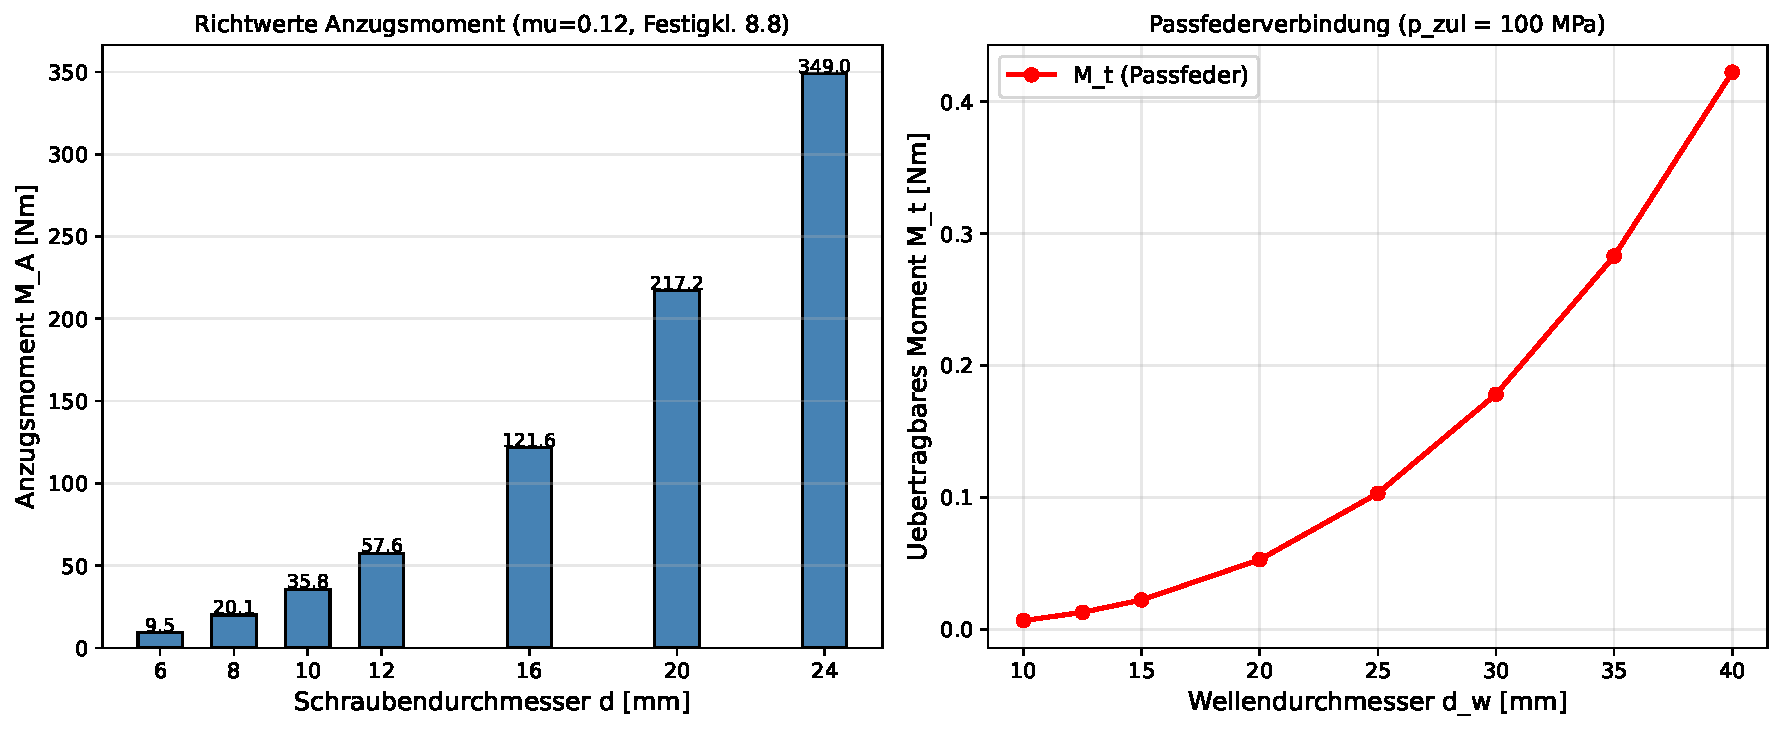
\includegraphics[width=0.90\textwidth]{plot_maschinenelemente.pdf}
\caption{Links: Richtwerte des Anzugsmoments f\"ur Schrauben der
Festigkeitsklasse 8.8 ($\mu = 0{,}12$) -- superlineares Wachstum mit dem Durchmesser.
Rechts: \"Ubertragbares Torsionsmoment einer Passfederverbindung
($p_{zul} = 100\,\mathrm{MPa}$) in Abh\"angigkeit des Wellendurchmessers.}
\label{fig:maschinenelemente}
\end{figure}

\begin{satz}[Schraubenkraftanalyse -- VDI 2230]
In einer vorgespannten Schraubenverbindung mit Vorspannkraft $F_V$,
\"au\ss{}erer axialer Betriebslast $F_B$ und Verspannungskoeffizient:
\[
  \Phi = \frac{\delta_P}{\delta_S + \delta_P},
\]
gilt f\"ur die Schraubenzusatzkraft $F_{SA}$ und die Restklemmkraft $F_{KR}$:
\[
  F_{SA} = \Phi\,F_B, \qquad F_{KR} = F_V - (1-\Phi)F_B.
\]
Die Verbindung \"offnet (klafft) wenn $F_{KR} \le 0$, d.\,h. wenn $F_B > F_V/(1-\Phi)$.
\end{satz}
\begin{proof}
Im Verspannungsdreieck wirken Schraube und Klemmt\"eile wie Federn in Reihe
(von der Verbindung aus gesehen) bzw. in Parallel (bzgl. der \"au\ss{}eren Last).
Die Steifigkeiten sind $c_S = 1/\delta_S$ (Schraube) und $c_P = 1/\delta_P$ (Klemmt\"eil).
Mit der Kompatibilit\"atsbedingung (gleiche Verformungs\"anderung) und der
Gleichgewichtsbedingung folgen die angegebenen Ausdr\"ucke.
\end{proof}

\section{Welle-Nabe-Verbindungen}

\begin{definition}[Passfederverbindung nach DIN 6885]
Eine \textbf{Passfeder} (Breite $b$, H\"ohe $h$, L\"ange $l$) \"ubertr\"agt das
Moment $M_t$ durch Fl\"achenpressung $p$ auf den Seitenfl\"achen:
\[
  M_t \le p_{zul}\,l_t\,\frac{h-t_1}{2}\cdot\frac{d}{2},
  \quad l_t \approx l - b\;(\text{tragende L\"ange}).
\]
Passfedern sind einfach montierbar, aber nicht drehmoment-stoß-fest.
Typische Zul\"assige Fl\"achenpressung:
Stahl/Stahl $p_{zul} = 100\ldots150\,\mathrm{MPa}$; Stahl/Gusseisen $70\ldots100\,\mathrm{MPa}$.
\end{definition}

\begin{definition}[Pressverbindungen]
Bei \textbf{Pressverbindungen} (Welle $> $ Naben-Bohrung) entsteht durch
elastische Aufweitung der Nabe und Zusammendr\"uckung der Welle ein Fugendruck $p_F$:
\[
  p_F = \frac{U}{d}\cdot\frac{E}{(Q_A^2+1)/(Q_A^2-1) + (Q_I^2+1)/(Q_I^2-1) + \nu_A + \nu_I},
\]
mit dem \"Uberma\ss{} $U$ (Differenz der Durchmesser), den Durchmesserverh\"altnissen
$Q_A = D_A/d$ (Nabe) und $Q_I = d/d_I$ (Vollwelle: $Q_I \to \infty$).
Das \"ubertragbare Moment: $M_t = \mu_F\,p_F\,\pi d^2 L/2$.
\end{definition}

\section{W\"alzlager}

\begin{definition}[W\"alzlager -- Typen und Belastbarkeit]
W\"alzlager unterst\"utzen Wellen durch rollende Elemente (Kugeln, Zylinder,
Kegel, Nadeln) und erm\"oglichen freie Rotation mit minimalem Reibmoment.
Klassifikation:
\begin{itemize}
    \item[-] \textbf{Rillenkugellager} (DIN 625): allseitig belastbar; hohe Drehzahl
    \item[-] \textbf{Pendelkugellager}: selbstausrichtend; toleriert Flucht-fehler
    \item[-] \textbf{Zylinderrollenlager}: hohe radiale Tragf\"ahigkeit; kein Axiallast
    \item[-] \textbf{Kegelrollenlager}: kombinierte Radial- und Axiallast (Fahrzeug-Naben)
    \item[-] \textbf{Schr\"agkugellager}: gezielt f\"ur Axiallast (Spindellager)
    \item[-] \textbf{Nadellager}: sehr kleine Bauh\"ohe (Kardanwellen, Kipphebel)
\end{itemize}
\end{definition}

\begin{satz}[W\"alzlager-Lebensdauer nach ISO 281]
Die nominelle Lagerlebensdauer $L_{10}$ (in $10^6$ Umdrehungen) bei der
$10\,\%$ der Lager ausf\"allen:
\[
  L_{10} = \left(\frac{C}{P}\right)^p,
  \quad
  L_{10h} = \frac{10^6}{60\,n}\left(\frac{C}{P}\right)^p\;[\mathrm{h}].
\]
Exponent: $p = 3$ (Kugellager), $p = 10/3$ (Rollenlager).
Die \textbf{\"aquivalente dynamische Lagerbelastung}:
$P = X F_r + Y F_a$ ($X, Y$: Faktoren aus Hersteller-Tabelle).
\end{satz}
\begin{proof}
Die ISO-281-Formel basiert auf der Hertz'schen Kontaktspannung und dem
Materialermuedungsmodell nach Lundberg und Palmgren (1947): Die
Ermuedungslebensdauer skaliert mit der Kontaktkraft $Q$ gem\"a\ss{}
$L \propto Q^{-c}$ ($c \approx 3$ f\"ur Punktkontakt/Kugeln).
Die dynamische Tragzahl $C$ ist die Last, bei der $L_{10} = 10^6$ Umd.
\end{proof}

\section{Zahnradgetriebe}

\begin{definition}[Evolventenverzahnung und Eingriffsverhältnisse]
Das wichtigste Verzahnungsprinzip im Maschinenbau ist die
\textbf{Evolventenverzahnung} (DIN 867): Der Zahnprofil ist eine Evolvente
des Grundkreises ($r_b = r\cos\alpha_0$, mit Teilkreisradius $r$ und
Eingriffswinkel $\alpha_0 = 20^\circ$ standardm\"a\ss{}ig).

\"Ubersetzungsverh\"altnis zweier Stirnr\"ader (Z\"ahnezahl $z_1$, $z_2$,
Teilkreisradius $r_1$, $r_2$):
\[
  i = \frac{\omega_1}{\omega_2} = \frac{z_2}{z_1} = \frac{r_2}{r_1}.
\]
Modul: $m = d/z = 2r/z$ (DIN 780: normierte Modulgr\"o\ss{}en 1, 1{,}25, 1{,}5, 2, 2{,}5, \ldots)
\end{definition}

\begin{satz}[Hertz'sche Pressung am Zahnkontakt]
Die maximale Hertz'sche Pressung im Zahnflankenkontakt
(zylindrische Evolventen-Stirnr\"ader):
\[
  p_{H,\max} = Z_E\sqrt{\frac{F_t}{b\,d_1}\cdot\frac{i+1}{i\cdot u_0}},
\]
mit dem Elastizit\"atszahl $Z_E = \sqrt{E_r/\pi}$ (reduzierter E-Modul
$E_r = E/(1-\nu^2)$ f\"ur symmetrische Materialien), Zahnbreite $b$,
Teilkreisdurchmesser $d_1$ und geometrischem Kontaktterm $u_0$.
\end{satz}

\section{Federn und D\"ampferelemente}

\begin{definition}[Federtypen und Federkonstanten]
\begin{itemize}
    \item[-] \textbf{Schraubenzugfeder} (Zug): $c = \frac{G d_D^4}{8 D_m^3 n}$ (D\"unndraht-N\"aherung)
    \item[-] \textbf{Blattfeder}: $c = \frac{E b h^3}{4L^3}$ (einseitig eingespannt)
    \item[-] \textbf{Tellerfeder} (Bellevue): hohe Kraft auf kleinem Weg; stapelbar
    \item[-] \textbf{Torsionsstabfeder}: $c_\phi = GI_p/L$ (winkelsteife Lagerung)
    \item[-] \textbf{Gummifeder}: nichtlinear; hohe D\"ampfung; korrosionsunempfindlich
\end{itemize}
Zwei Federn in Reihe: $1/c_{ges} = 1/c_1 + 1/c_2$.
Zwei Federn parallel: $c_{ges} = c_1 + c_2$.
\end{definition}

\begin{satz}[Energiespeicherung in Federn]
Die in einer linear-elastischen Feder gespeicherte potenzielle Energie:
$E_{pot} = \tfrac{1}{2}cF^2 = \tfrac{1}{2}cx^2$.
Das \textbf{spezifische Federvolumen} (gespeicherte Energie pro Masse)
einer Schraubenzugfeder:
\[
  \frac{E_{pot}}{m} = \frac{\tau_{\max}^2}{4G\rho} \quad
  (\text{h\"ochste Werte f\"ur Federstahl: bis } 60\,\mathrm{Wh/kg}).
\]
\end{satz}

% ============================================================

\section{Getriebetechnik und Antriebsstränge}

\begin{definition}[Getriebebauarten und Wirkungsgrade]
Getriebe wandeln Drehzahl und Drehmoment um. Wichtige Bauarten:
\begin{itemize}
    \item[-] \textbf{Stirnradgetriebe}: parallele Achsen; hoher Wirkungsgrad
          $\eta \approx 0{,}98\ldots0{,}99$ pro Stufe; große Übersetzungsbandbreite
    \item[-] \textbf{Kegelradgetriebe}: schneidende Achsen (meist $90^\circ$);
          $\eta \approx 0{,}97\ldots0{,}99$; Fahrzeugachsen, Differentiale
    \item[-] \textbf{Schneckengetriebe}: windschiefe Achsen; große Übersetzungen
          ($i = 5\ldots80$ pro Stufe); Selbsthemmung möglich;
          $\eta \approx 0{,}60\ldots0{,}90$ (schlecht bei kleinem Steigungswinkel)
    \item[-] \textbf{Planetengetriebe}: kompakt, hohe Leistungsdichte;
          $\eta \approx 0{,}96\ldots0{,}99$; Automatikgetriebe, Windgetriebe
    \item[-] \textbf{Harmonic-Drive}: tordierte Stahlflexspline;
          Übersetzung bis $i = 320$; spielfrei; Robotergelenke
\end{itemize}
Mehrstufige Getriebe: $\eta_{ges} = \prod_k \eta_k$;
Gesamtübersetzung: $i_{ges} = \prod_k i_k$.
\end{definition}

\begin{satz}[Planetengetriebe -- Willis-Gleichung]
Für ein Planetengetriebe mit Sonnenrad ($z_s$), Planetenrad ($z_p$),
Hohlrad ($z_h$) und Steg gilt die \textbf{Willis-Gleichung}:
\[
  \frac{\omega_s - \omega_0}{\omega_h - \omega_0} = -\frac{z_h}{z_s},
\]
wobei $\omega_0$ die Stegdrehzahl ist. Für festgehaltenes Hohlrad
($\omega_h = 0$): $\omega_s/\omega_0 = 1 + z_h/z_s$ (Standübersetzung $i_0 = -z_h/z_s$).
\end{satz}
\begin{proof}
Im mit dem Steg umlaufenden Bezugssystem (Stegdrehzahl subtrahiert)
liegt ein einfaches Stirnradgetriebe: $(\omega_s - \omega_0)/(\omega_h - \omega_0) = i_0$.
Da Sonnenrad und Hohlrad über die Planeten im äußeren Eingriff stehen
(Hohlrad: Innenverzahnung): $i_0 = -z_h/z_s$ (Vorzeichenwechsel durch Inneneingriff).
\end{proof}

\section{Technische Akustik -- Schalldämmung und Absorption}

\begin{definition}[Schalldämm-Maß und Absorptionsgrad]
Das \textbf{Schalldämm-Maß} $R$ einer Trennwand (Masse $m''$ [kg/m$^2$]):
\[
  R \approx 20\log_{10}(f\cdot m'') - 47\,\mathrm{dB} \quad (\text{Massegesetz}),
\]
d.\,h. Verdoppelung der flächenbezogenen Masse erhöht $R$ um $6\,\mathrm{dB}$;
Verdoppelung der Frequenz ebenfalls $+6\,\mathrm{dB}$.

Der \textbf{Absorptionsgrad} $\alpha$ eines Materials:
\[
  \alpha = \frac{\text{absorbierte Schallleistung}}{\text{auftreffende Schallleistung}} \in [0,1].
\]
Poröse Materialien (Mineralwolle, Schaumstoff): $\alpha \to 1$ bei hohen Frequenzen.
Glatte Betonwand: $\alpha \approx 0{,}01$ (fast vollständige Reflexion).
\end{definition}

\begin{beobachtung}[Aktive Geräuschunterdrückung (ANC)]
\textbf{Active Noise Control} (ANC) erzeugt ein Gegenschallfeld,
das durch destruktive Interferenz den Lärm auslöscht.
Prinzip: Mikrofon misst Störgeräusch $x(n)$; adaptiver Filter
(LMS-Algorithmus) berechnet Gegensignal $y(n) = -\hat{H}\{x(n)\}$;
Fehlermikrofon misst Restsignal $e(n) \to 0$.
Der \textbf{LMS-Algorithmus} (Least Mean Squares) passt die Filterkoeffizienten
$\vec{w}$ adaptiv an:
\[
  \vec{w}_{k+1} = \vec{w}_k + 2\mu\,e(k)\,\vec{x}(k),
\]
mit Schrittweite $\mu$ (Konvergenzparameter).
Anwendungen: Kopfhörer mit ANC, Kraftfahrzeug-Innenraum-Akustik (Road Noise ANC).
\end{beobachtung}

\section{Mechatronik und integrierter Systementwurf}

\begin{definition}[Mechatronisches System]
\textbf{Mechatronik} (Mechanik + Elektronik + Informatik) beschreibt
die synergetische Integration mechanischer, elektronischer und
informationstechnischer Komponenten zu einem optimierten Gesamtsystem.
V-Modell des mechatronischen Entwicklungsprozesses:
\begin{itemize}
    \item[-] \textbf{Anforderungen} $\to$ \textbf{Systemarchitektur}
    \item[-] \textbf{Teilsystemdesign} (Mechanik, Elektronik, Software parallel)
    \item[-] \textbf{Verifikation} jeder Ebene (Simulation $\to$ Hardware-in-the-Loop $\to$ Prototyp $\to$ Serientest)
\end{itemize}
Schlüsselwerkzeuge: MATLAB/Simulink, dSPACE Rapid Prototyping,
AUTOSAR-Softwarearchitektur, SPICE (Elektronik-Simulation).
\end{definition}

\begin{beobachtung}[Hardware-in-the-Loop (HiL) Simulation]
In der \textbf{HiL-Simulation} wird ein reales Steuergerät (ECU)
mit einer Echtzeitsimulation der Regelstrecke verbunden:
\begin{itemize}
    \item[-] Simulationslaufzeit $< 1\,\mathrm{ms}$ (Echtzeit-Constraint)
    \item[-] Elektrische Signalschnittstellen emulieren Sensoren und Aktoren
    \item[-] Fehlersimulation (Kurzschlüsse, Kabelbrüche) für Robustheitstests
    \item[-] Gesetzlich vorgeschrieben für sicherheitskritische ECUs (Bremse, ESP, Airbag)
\end{itemize}
HiL ermöglicht vollständige Erprobung vor dem ersten Fahrzeugprototypen --
typische Einsparung: $30\ldots50\,\%$ der Entwicklungskosten für Software-Tests.
\end{beobachtung}

\begin{beispiel}[Mechatronisches System: Elektromechanischer Aktor]
Ein elektromechanischer Linearaktor (Spindelantrieb) besteht aus:
PMSM ($P = 2\,\mathrm{kW}$, $n_{max} = 3000\,\mathrm{min^{-1}}$, $M_{max} = 10\,\mathrm{Nm}$)
+ Kugelgewindetrieb (Steigung $p_s = 10\,\mathrm{mm}$, Wirkungsgrad $\eta_{KGT} = 0{,}95$).

Maximale Axialkraft:
\[
  F_{ax} = \frac{2\pi\eta_{KGT}\,M_{max}}{p_s} = \frac{2\pi\cdot0{,}95\cdot10}{0{,}01} \approx 5969\,\mathrm{N}.
\]
Maximale Lineargeschwindigkeit:
\[
  v_{max} = \frac{n_{max}\cdot p_s}{60} = \frac{3000\cdot0{,}01}{60} = 0{,}5\,\mathrm{m/s}.
\]
Gesamtsteifigkeit (Welle + Mutter):
$c_{ges} = 1/(1/c_{Welle} + 1/c_{Mutter}) \approx 300\,\mathrm{N/\mu m}$.
Eigenfrequenz des Antriebsstrangs:
$f_0 = \frac{1}{2\pi}\sqrt{c_{ges}/m_{eff}} \approx 220\,\mathrm{Hz}$ (typisch).
\end{beispiel}

\chapter{Schwingungslehre}
% ============================================================

Die Schwingungslehre befasst sich mit periodischen oder quasi-periodischen
Bewegungen mechanischer Systeme. Schwingungen k\"onnen erw\"unscht sein
(Schwingf\"order, Ultraschallreinigung) oder gef\"ahrlich
(Resonanzkatastrophen, Erm\"udungsversagen).

\section{Freie unged\"ampfte Schwingungen}

\begin{definition}[Einmassenschwinger]
Das einfachste Schwingungsmodell ist der \textbf{lineare Einmassenschwinger}:
eine Punktmasse $m$ an einer Feder $c$ (ohne D\"ampfung):
\[
  m\,\ddot{x} + c\,x = 0, \qquad x(0) = x_0, \quad \dot{x}(0) = v_0.
\]
\end{definition}

\begin{satz}[L\"osung der freien unged\"ampften Schwingung]
Die allgemeine L\"osung ist:
\[
  x(t) = A\cos(\omega_0 t - \varphi_0),
\]
mit der \textbf{Eigenfrequenz} $\omega_0 = \sqrt{c/m}$, der Amplitude
$A = \sqrt{x_0^2 + (v_0/\omega_0)^2}$ und der Phasenlage
$\tan\varphi_0 = -v_0/(\omega_0 x_0)$.
\end{satz}
\begin{proof}
Charakteristisches Polynom: $m\lambda^2 + c = 0 \Rightarrow \lambda = \pm i\omega_0$.
Allgemeine L\"osung: $x(t) = C_1 e^{i\omega_0 t} + C_2 e^{-i\omega_0 t}
= B_1\cos\omega_0 t + B_2\sin\omega_0 t$.
Anfangsbedingungen: $B_1 = x_0$, $B_2 = v_0/\omega_0$.
Umschreiben als $A\cos(\omega_0 t - \varphi_0)$ mit
$A = \sqrt{B_1^2 + B_2^2}$ und $\tan\varphi_0 = B_2/B_1$.
\end{proof}

\section{Freie ged\"ampfte Schwingungen}

\begin{definition}[D\"ampfungsgr\"o\ss{}en]
Mit viskosem D\"ampfer $d$ (Kraft proportional zur Geschwindigkeit):
$m\ddot{x} + d\dot{x} + cx = 0$.
Das \textbf{Lehr'sche D\"ampfungsma\ss{}}:
\[
  D = \frac{d}{d_{krit}} = \frac{d}{2\sqrt{mc}} = \frac{d}{2m\omega_0},
  \qquad d_{krit} = 2\sqrt{mc}.
\]
\end{definition}

\begin{satz}[L\"osungsf\"alle der ged\"ampften Schwingung]
Die L\"osung h\"angt von $D$ ab (charakteristische Gleichung $\lambda^2 + 2D\omega_0\lambda + \omega_0^2 = 0$):
\begin{itemize}
    \item[-] $D < 1$ (\textbf{Unterd\"ampfung}):
          $x(t) = e^{-D\omega_0 t}(C_1\cos\omega_d t + C_2\sin\omega_d t)$,
          $\omega_d = \omega_0\sqrt{1-D^2}$ (ged\"ampfte Eigenfrequenz)
    \item[-] $D = 1$ (\textbf{aperiodischer Grenzfall}):
          $x(t) = (C_1 + C_2 t)e^{-\omega_0 t}$ (schnellste D\"ampfung ohne \"Uberschwingen)
    \item[-] $D > 1$ (\textbf{\"Uberd\"ampfung}):
          $x(t) = C_1 e^{s_1 t} + C_2 e^{s_2 t}$,
          $s_{1,2} = -D\omega_0 \pm \omega_0\sqrt{D^2-1}$ (zwei negative Realwurzeln)
\end{itemize}
\end{satz}
\begin{proof}
Die Nullstellen des charakteristischen Polynoms sind
$\lambda_{1,2} = \omega_0(-D \pm \sqrt{D^2-1})$.
F\"ur $D < 1$: $\lambda_{1,2} = -D\omega_0 \pm i\omega_d$ (komplex-konjugiert).
Mit der Euler-Formel folgt die erste L\"osungsform.
F\"ur $D = 1$: Doppelnullstelle $\lambda = -\omega_0$; die L\"osung bei
Doppelnullstelle lautet $(C_1 + C_2 t)e^{\lambda t}$.
F\"ur $D > 1$: Zwei reelle Nullstellen; direkte Superposition.
\end{proof}

\section{Erzwungene Schwingungen}

\begin{satz}[Station\"are Amplitude bei harmonischer Erregung]
F\"ur die erzwungene Schwingung $m\ddot{x} + d\dot{x} + cx = F_0\cos\Omega t$
ist die station\"are Amplitude:
\[
  x_A = \frac{F_0/c}{\sqrt{(1-\eta^2)^2 + (2D\eta)^2}} = \frac{F_0}{c}\,V(\eta,D),
\]
mit dem Frequenzverh\"altnis $\eta = \Omega/\omega_0$ und der
\textbf{Vergr\"o\ss{}erungsfunktion} $V(\eta, D)$.
Die Resonanzamplitude ($\eta \approx 1$, $D \ll 1$): $V_{\max} \approx 1/(2D)$.
\end{satz}
\begin{proof}
Stationaerer Ansatz $x_p = A\cos(\Omega t - \varphi)$ einsetzen:
$(c - m\Omega^2)A\cos\varphi - d\Omega A\sin\varphi = F_0$,
$(c - m\Omega^2)A\sin\varphi + d\Omega A\cos\varphi = 0$.
Quadrieren und addieren: $A^2[(c-m\Omega^2)^2 + (d\Omega)^2] = F_0^2$.
Division durch $c^2$ und Einf\"uhren von $\eta$, $D$, $\omega_0$ liefert die Formel.
Das Maximum von $V$ bei $\mathrm{d}V/\mathrm{d}\eta = 0$:
$\eta_{\text{res}} = \sqrt{1-2D^2}$; $V_{\max} = 1/(2D\sqrt{1-D^2})$.
\end{proof}

\begin{figure}[htbp]
\centering
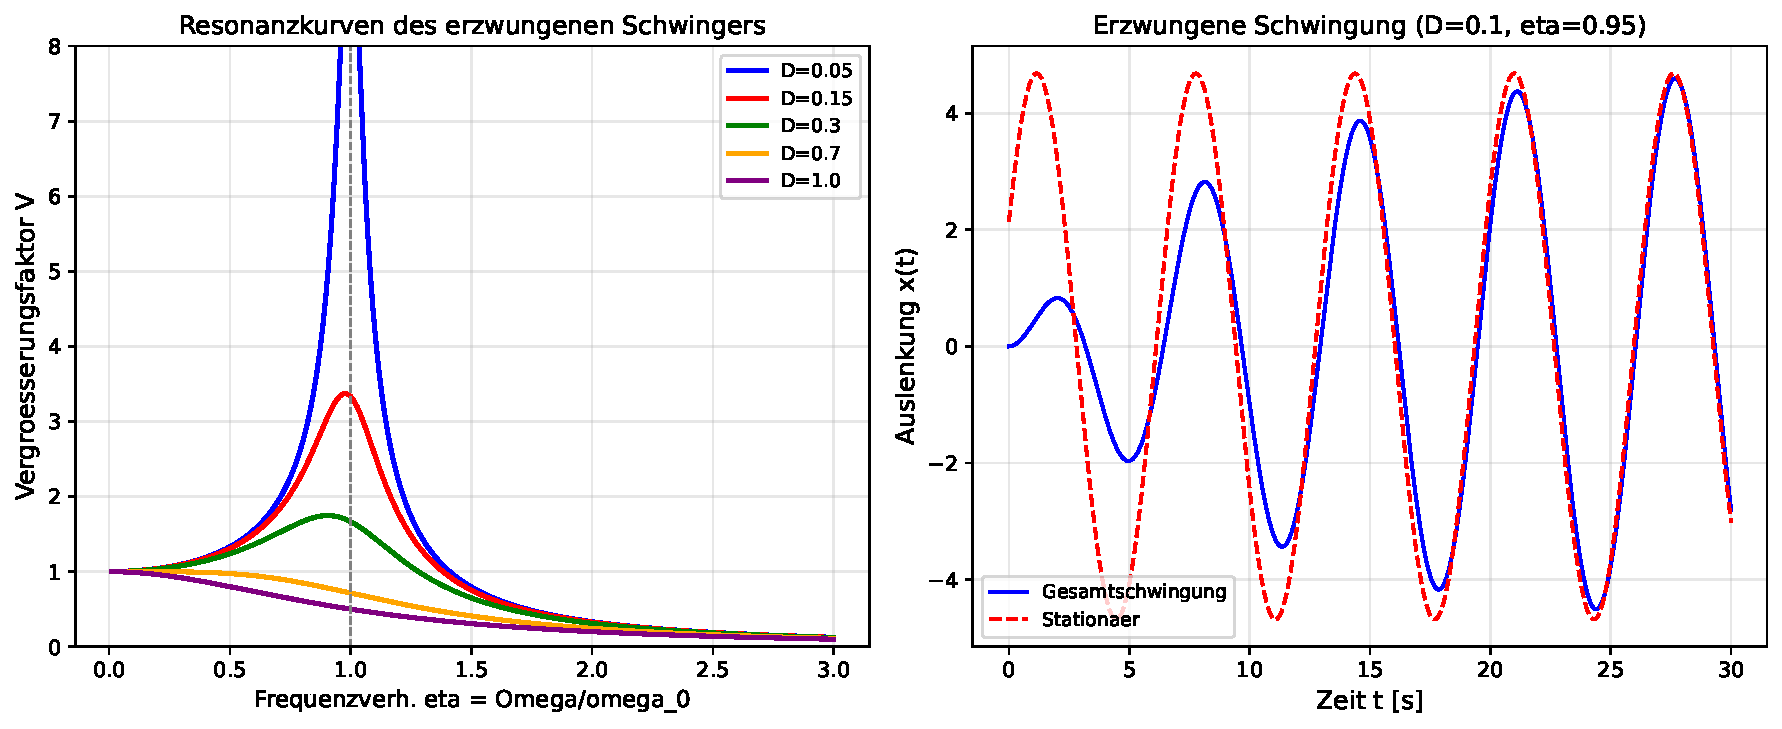
\includegraphics[width=0.92\textwidth]{plot_schwingung.pdf}
\caption{Links: Resonanzkurven des erzwungenen Schwingers f\"ur verschiedene
D\"ampfungsgrade $D$. F\"ur $D = 0{,}05$ (blau) entsteht eine starke Resonanzspitze.
Rechts: Zeitlicher Verlauf bei $D = 0{,}1$ und $\eta = 0{,}95$ -- nach dem
Einschwingvorgang dominiert die station\"are Schwingung.}
\label{fig:schwingung}
\end{figure}

\section{Mehrfreiheitsgradsysteme und Modalanalyse}

\begin{definition}[Schwingungsgleichung in Matrixform]
F\"ur ein System mit $n$ Freiheitsgraden gelten die \textbf{Bewegungsgleichungen}:
\[
  \mathbf{M}\,\ddot{\vec{x}} + \mathbf{D}\,\dot{\vec{x}} + \mathbf{K}\,\vec{x} = \vec{F}(t),
\]
mit symmetrischer, positiv definiter Massenmatrix $\mathbf{M}$,
D\"ampfungsmatrix $\mathbf{D}$ und symmetrischer, positiv semi-definiter
Steifigkeitsmatrix $\mathbf{K}$.
\end{definition}

\begin{satz}[Eigenwertproblem und Modalanalyse]
Die Eigenfrequenzen $\omega_k$ des unged\"ampften Systems
($\mathbf{D} = \mathbf{0}$) sind die L\"osungen des \textbf{verallgemeinerten Eigenwertproblems}:
\[
  (\mathbf{K} - \omega_k^2\,\mathbf{M})\,\vec{\phi}_k = \vec{0},
  \qquad k = 1, \ldots, n.
\]
Die Eigenformen $\vec{\phi}_k$ sind $\mathbf{M}$-orthogonal:
\[
  \vec{\phi}_i^\top\mathbf{M}\vec{\phi}_j = \delta_{ij} m_k \quad (\text{modales Massenmatrix}),
  \qquad \vec{\phi}_i^\top\mathbf{K}\vec{\phi}_j = \delta_{ij}\omega_k^2 m_k.
\]
\end{satz}
\begin{proof}
Aus $\mathbf{K}\vec{\phi}_i = \omega_i^2\mathbf{M}\vec{\phi}_i$ und
$\mathbf{K}\vec{\phi}_j = \omega_j^2\mathbf{M}\vec{\phi}_j$ folgt durch
Pr\"amultiplikation mit $\vec{\phi}_j^\top$ bzw. $\vec{\phi}_i^\top$
und Subtraktion (Symmetrie von $\mathbf{K}$ und $\mathbf{M}$):
$(\omega_i^2 - \omega_j^2)\vec{\phi}_j^\top\mathbf{M}\vec{\phi}_i = 0$.
F\"ur $\omega_i \neq \omega_j$: $\vec{\phi}_j^\top\mathbf{M}\vec{\phi}_i = 0$.
\end{proof}

\begin{beobachtung}[Anwendungen der Modalanalyse]
Die Modalanalyse hat weit \"uber die Maschinendynamik hinaus gro\ss{}e Bedeutung:
In der Strukturdynamik gro\ss{}er Systeme (Geb\"aude, Br\"ucken, Flugzeuge) werden
die Eigenfrequenzen und -formen durch experimentelle Modalanalyse
(Beschleunigungssensoren, Impulshammer oder Shaker) bestimmt.
Die gemessenen Modenformen erm\"oglichen:
\begin{itemize}
    \item[-] Detektion von Sch\"aden (Risse ver\"andern Steifigkeits-matrix $\mathbf{K}$)
    \item[-] Validierung von FEM-Modellen
    \item[-] Auslegung von schwingungsminderenden Ma\ss{}nahmen
          (Tilger, D\"ampfer, Strukturmodifikation)
    \item[-] Lebensdauerprognose unter dynamischer Betriebslast
\end{itemize}
\end{beobachtung}

\section{Schwingungsisolation und Tilger}

\begin{satz}[Krafttransmissionsgrad]
Der \textbf{Krafttransmissionsgrad} $\eta_T$ gibt an, welcher Anteil
der Erregerkraft auf das Fundament \"ubertragen wird:
\[
  \eta_T = \frac{F_{\text{Fundament}}}{F_0} = V(\eta,D)\sqrt{1 + (2D\eta)^2}.
\]
F\"ur $\eta > \sqrt{2}$ ist $\eta_T < 1$: Die Feder-D\"ampfer-Isolation
reduziert die Kraft\"ubertragung. Optimale Isolation: kleine $D$ und gro\ss{}es $\eta$
(weiche Lagerung, d.\,h. $\omega_0 \ll \Omega$).
\end{satz}

\begin{definition}[Schwingungstilger (Absor-ber)]
Ein \textbf{dynamischer Schwingungstilger} (Masse $m_T$, Feder $c_T$,
auf die Hauptmasse $M$ montiert) erz\"ugt bei der Tilgerfrequenz
$\omega_T = \sqrt{c_T/m_T} = \omega_0$ eine vollst\"andige Ausl\"oschung
der Hauptmassenschwingung (im unged\"ampften Fall).
Im ged\"ampften Tilger (Lanchester-Tilger, 1928) verschwindet die
Resonanzspitze weitgehend bei optimaler D\"ampfung
$D_{T,\text{opt}} = \sqrt{3\mu/(8(1+\mu)^3)}$ (Masseverh\"altnis $\mu = m_T/M$).
\end{definition}

% ============================================================
\chapter{Regelungstechnik}
% ============================================================

Die Regelungstechnik sorgt daf\"ur, dass eine Maschine trotz
St\"orungen und Unsicherheiten das gew\"unschte Verhalten zeigt.
Der geschlossene Regelkreis ist das zentrale Paradigma: Durch
kontinuierliche R\"uckkopplung der gemessenen Ausgangsgr\"o\ss{}e
wird der Regler st\"andig nachjustiert.

\section{Modellierung linearer dynamischer Systeme}

\begin{definition}[Laplace-Transformation und \"Ubertragungsfunktion]
Die \textbf{Laplace-Transformation} \"uberf\"uhrt Zeitfunktionen in
den komplexen Frequenzbereich ($s = \sigma + i\omega$):
\[
  F(s) = \mathcal{L}\{f(t)\} = \int_0^\infty f(t)\,e^{-st}\,\mathrm{d}t.
\]
Wichtige Korrespondenzen:
\begin{center}
\begin{tabular}{lll}
\toprule
$f(t)$ & $F(s)$ & Bemerkung \\
\midrule
$\delta(t)$ & $1$ & Dirac-Impuls \\
$\sigma(t)$ & $1/s$ & Sprungfunktion \\
$e^{-at}$ & $1/(s+a)$ & exponentielle Abklingung \\
$\sin(\omega t)$ & $\omega/(s^2+\omega^2)$ & Sinus \\
$f'(t)$ & $sF(s) - f(0)$ & Differentiationsregel \\
$\int_0^t f\,\mathrm{d}\tau$ & $F(s)/s$ & Integrationsregel \\
\bottomrule
\end{tabular}
\end{center}
Die \textbf{\"Ubertragungsfunktion} $G(s) = Y(s)/U(s)$ beschreibt
das Eingangs-Ausgangs-Verhalten eines LZI-Systems.
\end{definition}

\begin{definition}[Standardglieder der Regelungstechnik]
\begin{itemize}
    \item[-] \textbf{P-Glied}: $G(s) = K_P$; statisch, frequenzunabh\"angig
    \item[-] \textbf{I-Glied}: $G(s) = 1/(T_I s)$; stationaere Genauigkeit, Phasennacheilung $-90^\circ$
    \item[-] \textbf{D-Glied}: $G(s) = T_D s$; Phasenvoreilung $+90^\circ$; rein differenzierend (nicht realisierbar)
    \item[-] \textbf{PT1-Glied}: $G(s) = K/(1+Ts)$; Verz\"ogerung 1. Ordnung; $\tau_{63\%} = T$
    \item[-] \textbf{PT2-Glied}: $G(s) = K\omega_0^2/(s^2 + 2D\omega_0 s + \omega_0^2)$
    \item[-] \textbf{Tt-Glied}: $G(s) = e^{-Tt s}$ (Totzeitglied, nicht-minimal-phasig)
\end{itemize}
\end{definition}

\begin{satz}[Pol-Nullstellen-Darstellung und Stabilit\"at]
Die \"Ubertragungsfunktion $G(s)$ eines Systems $n$-ter Ordnung:
\[
  G(s) = K\,\frac{\prod_{j=1}^m (s - z_j)}{\prod_{i=1}^n (s - p_i)},
\]
mit Nullstellen $z_j$ (Z\"ahler) und Polen $p_i$ (Nenner).
Das System ist \textbf{BIBO-stabil} (bounded input -- bounded output)
genau dann, wenn alle Pole negativen Realteil haben: $\text{Re}(p_i) < 0$.
\end{satz}
\begin{proof}
Die Impulsantwort $g(t) = \mathcal{L}^{-1}\{G(s)\}$ ist eine Superposition
von Termen der Form $t^k e^{p_i t}$ (Partialbruchzerlegung).
Diese Terme klingen genau dann f\"ur $t\to\infty$ ab ($g(t) \to 0$),
wenn $\text{Re}(p_i) < 0$ f\"ur alle $i$.
BIBO-Stabilit\"at \"aquivalent zu $\int_0^\infty |g(t)|\,\mathrm{d}t < \infty$,
was genau f\"ur $\text{Re}(p_i) < 0$ gilt.
\end{proof}

\section{Analyse im Frequenzbereich}

\begin{satz}[Hurwitz-Kriterium -- algebraische Stabilit\"atsbedingung]
Das charakteristische Polynom $P(s) = a_n s^n + \cdots + a_1 s + a_0$
($a_i > 0$) hat alle Wurzeln mit negativem Realteil (stabiles System)
genau dann, wenn alle Hurwitz-Determinanten positiv sind:
\[
  H_1 = a_{n-1} > 0, \quad
  H_2 = \begin{vmatrix} a_{n-1} & a_n \\ a_{n-3} & a_{n-2}\end{vmatrix} > 0, \quad \ldots
\]
\end{satz}
\begin{proof}
Der Beweis von Hurwitz (1895) zeigt \"Aquivalenz mit dem Routh-Schema.
Das Routh-Array wird aus den Polynomkoeffizienten aufgebaut;
ein Vorzeichenwechsel in der ersten Spalte entspricht einem Pol mit
positivem Realteil. Die Zahl der Vorzeichenwechsel gibt die Anzahl
der instabilen Pole.
\end{proof}

\begin{figure}[htbp]
\centering
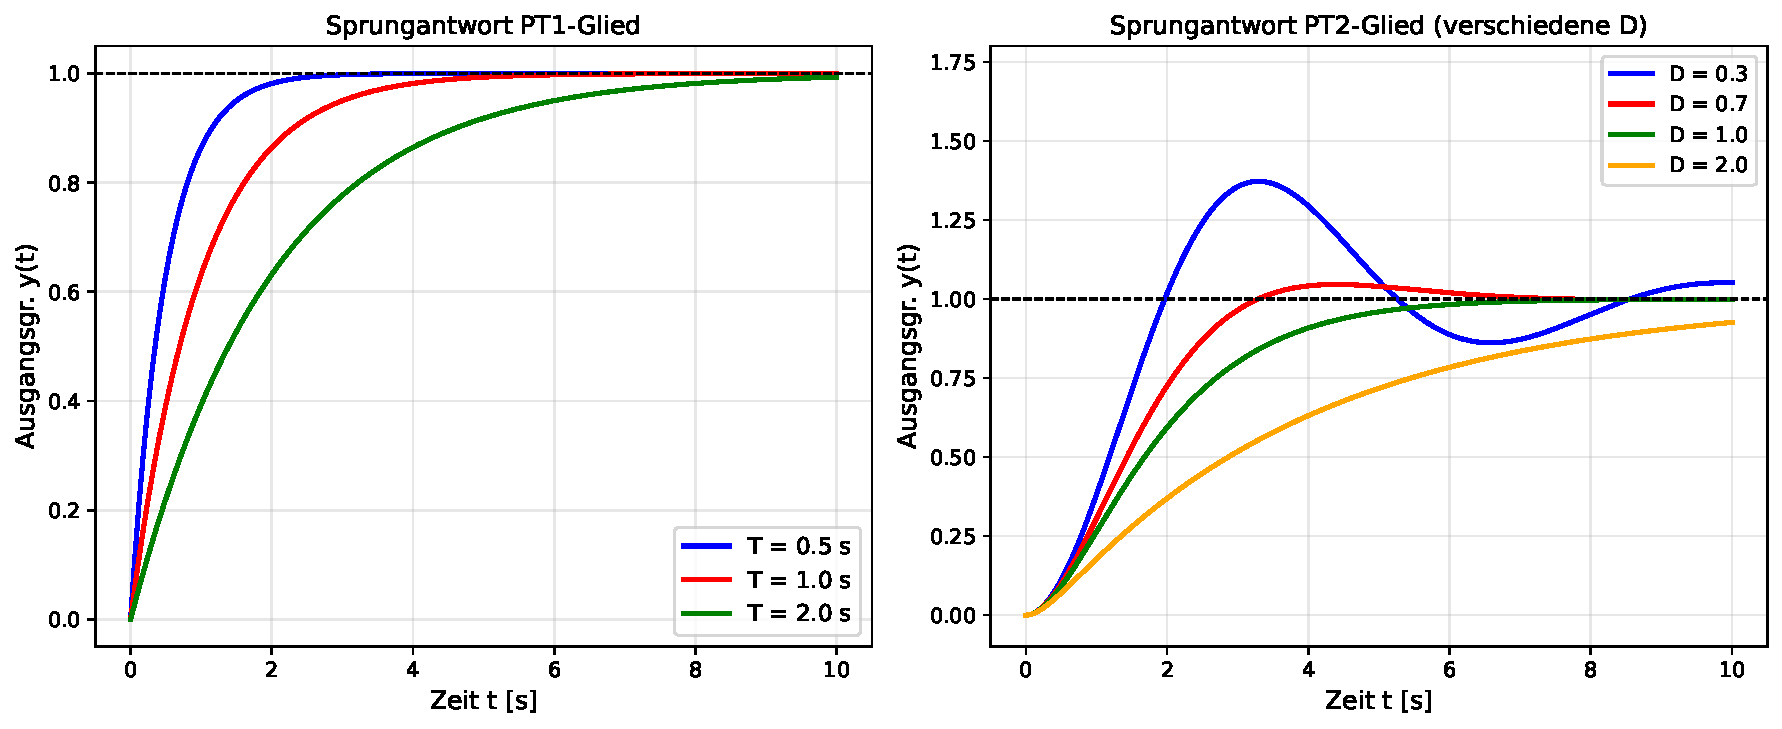
\includegraphics[width=0.92\textwidth]{plot_regelung.pdf}
\caption{Links: Sprungantworten des PT1-Gliedes f\"ur $T = 0{,}5$, $1{,}0$ und $2{,}0\,\mathrm{s}$
-- nach $5T$ ist der station\"are Endwert praktisch erreicht.
Rechts: Sprungantworten des PT2-Gliedes f\"ur verschiedene D\"ampfungen $D$
-- bei $D < 1$ schwingt das System \"uber (Unterd\"ampfung), $D = 1$ ist der aperiodische Grenzfall.}
\label{fig:regelung}
\end{figure}

\section{PID-Regler -- Auslegung und Einstellregeln}

\begin{definition}[PID-Regler]
Der \textbf{PID-Regler} kombiniert proportionalen, integralen und
differenzialen Anteil und ist der am h\"aufigsten eingesetzte Regler
in der industriellen Praxis:
\[
  u(t) = K_P\left[e(t) + \frac{1}{T_I}\int_0^t e(\tau)\,\mathrm{d}\tau + T_D\,\frac{\mathrm{d}e}{\mathrm{d}t}\right],
\]
mit der Regeldifferenz $e(t) = w(t) - y(t)$.
Im Bildbereich:
\[
  C(s) = K_P\left(1 + \frac{1}{T_I s} + T_D s\right)
       = K_P\frac{T_I T_D s^2 + T_I s + 1}{T_I s}.
\]
\end{definition}

\begin{beobachtung}[Einfluss der PID-Anteile]
Die drei Anteile des PID-Reglers haben unterschiedliche Wirkungen:
\begin{itemize}
    \item[-] \textbf{P-Anteil ($K_P$)}: proportionale Gegenwirkung; 
          gr\"o\ss{}eres $K_P$ erh\"oht Dynamik und Genauigkeit, aber
          senkt die Phasenreserve (\"Uberschwingen, Instabilit\"at)
    \item[-] \textbf{I-Anteil ($T_I$)}: eliminiert bleibende Regelabweichung;
          kleines $T_I$ beschleunigt Ausregelung, kann aber zu Schwingungen f\"uhren
    \item[-] \textbf{D-Anteil ($T_D$)}: reagiert auf schnelle \"Anderungen
          (Ableitung); verbessert Stabilit\"at bei tr\"agen Strecken;
          verst\"arkt Messrauschen (in Praxis mit Filter DT1 implementiert)
\end{itemize}
\end{beobachtung}

\begin{definition}[Ziegler-Nichols-Einstellregeln]
Die \textbf{kritische Methode} von Ziegler und Nichols (1942):
Man setzt $T_I = \infty$, $T_D = 0$ und erh\"oht $K_P$ bis zur
Dauerschwingung. Die kritische Verst\"arkung $K_{krit}$ und Schwingdauer $T_{krit}$
liefern Startwerte:
\begin{center}
\begin{tabular}{lccc}
\toprule
Reglertyp & $K_P$ & $T_I$ & $T_D$ \\
\midrule
P & $0{,}5\,K_{krit}$ & --- & --- \\
PI & $0{,}45\,K_{krit}$ & $0{,}83\,T_{krit}$ & --- \\
PID & $0{,}60\,K_{krit}$ & $0{,}50\,T_{krit}$ & $0{,}125\,T_{krit}$ \\
\bottomrule
\end{tabular}
\end{center}
\end{definition}

\section{Zustandsraumdarstellung}

\begin{definition}[Zustandsraummodell]
Ein LZI-System $n$-ter Ordnung wird durch die
\textbf{Zustandsraumdarstellung} beschrieben:
\[
  \dot{\vec{x}} = \mathbf{A}\vec{x} + \mathbf{B}\vec{u},
  \qquad \vec{y} = \mathbf{C}\vec{x} + \mathbf{D}\vec{u},
\]
mit Zustandsvektor $\vec{x} \in \mathbb{R}^n$, Eingangsvektor $\vec{u}$,
Ausgangsvektor $\vec{y}$, Systemmatrix $\mathbf{A}$,
Eingangsmatrix $\mathbf{B}$, Ausgangsmatrix $\mathbf{C}$
und Durchgangsmatrix $\mathbf{D}$.
Das System ist stabil $\Leftrightarrow$ alle Eigenwerte von $\mathbf{A}$ haben negativen Realteil.
\end{definition}

\begin{satz}[Zustandsregler (Polvorgabe)]
Ist das System $(A, B)$ vollst\"andig steuerbar, so kann durch
\textbf{Zustandsr\"uckf\"uhrung} $\vec{u} = -\mathbf{K}\vec{x}$
die Systemmatrix des geschlossenen Kreises
$\mathbf{A}_{cl} = \mathbf{A} - \mathbf{B}\mathbf{K}$
beliebige Eigenwerte erhalten (Polvorgabe).
\end{satz}
\begin{proof}
Vollst\"andige Steuerbarkeit bedeutet, dass die Steuer\-barkeitsmatrix
$\mathcal{S} = [\mathbf{B}, \mathbf{A}\mathbf{B}, \ldots, \mathbf{A}^{n-1}\mathbf{B}]$
vollen Rang hat (Kalman-Bedingung). Dann existiert nach dem Satz von
Ackermann ein $\mathbf{K}$, das jedes gew\"unschte charakteristische
Polynom von $\mathbf{A} - \mathbf{B}\mathbf{K}$ realisiert.
\end{proof}

% ============================================================
\chapter{Fertigungstechnik und Produktentwicklung}
% ============================================================

Fertigungstechnik umfasst alle Verfahren zur Herstellung und
Bearbeitung von Werkst\"ucken. Sie schlie\ss{}t das Bindeglied zwischen
Werkstoffwissenschaft (Was kann hergestellt werden?) und
Maschinenbau-Design (Was soll hergestellt werden?).

\section{Fertigungsverfahren nach DIN 8580}

\begin{definition}[Einteilung der Fertigungsverfahren]
DIN 8580 gliedert Fertigungsverfahren nach dem Formspeicher (Geometrieprinzip):
\begin{itemize}
    \item[-] \textbf{1. Urformen} (Masse- und Formzusammenhalt gleichzeitig erzeugen):
          Gie\ss{}en, Sintern, Laser-Pulver-Auftrag (Additive Fertigung)
    \item[-] \textbf{2. Umformen} (Formzusammenhalt erhalten, Form \"andern):
          Schmieden, Walzen, Tiefziehen, Strangpressen
    \item[-] \textbf{3. Trennen} (Formzusammenhalt vermindern):
          S\"agen, Fr\"asen, Drehen, Bohren, Schleifen (spanend);
          Wasserstrahlschneiden, Laserstrahl (nicht-spanend)
    \item[-] \textbf{4. F\"ugen} (Werkst\"ucke zusammensetzen):
          Schweissen, L\"oten, Kleben, Schrauben, Nieten
    \item[-] \textbf{5. Beschichten} (Oberfl\"achenschicht aufbringen):
          Galvanisieren, PVD/CVD (Hartstoffbeschichtung), Lackieren
    \item[-] \textbf{6. Stoffeigenschaften \"andern}: H\"arten, Gl\"uhen, Nitrieren
\end{itemize}
\end{definition}

\section{Spanende Fertigung}

\begin{definition}[Zerspanungskinematik -- Drehen]
Beim \textbf{Drehen} rotiert das Werkst\"uck mit der Drehzahl $n$ [min$^{-1}$],
w\"ahrend das Werkzeug sich axial mit dem Vorschub $f$ [mm/U] bewegt.
Wichtige Gr\"o\ss{}en:
\begin{itemize}
    \item[-] \textbf{Schnittgeschwindigkeit}: $v_c = \pi d n / 1000$ [m/min]
    \item[-] \textbf{Zeitspanvolumen}: $Q = f\cdot a_p\cdot v_c$ [$\mathrm{cm^3/min}$] ($a_p$: Schnitttiefe)
    \item[-] \textbf{Hauptzeit} (Maschinenzeit): $t_h = L/(f\cdot n)$ (Werkst\"uckenl\"ange $L$)
    \item[-] \textbf{Schnittkraft}: $F_c = k_{c1,1}\cdot b\cdot h^{(1-m_c)}$ (spez. Schnittkraft nach Kienzle)
\end{itemize}
\end{definition}

\begin{satz}[Taylor-Standzeit-Gleichung]
Die \textbf{Standzeit} $T$ (Zeit zwischen zwei Nachschleifen) h\"angt
von der Schnittgeschwindigkeit $v_c$ ab:
\[
  v_c\cdot T^m = C_T,
\]
mit Taylor-Exponent $m$ ($m \approx 0{,}2\ldots0{,}4$ f\"ur HSS;
$m \approx 0{,}2\ldots0{,}3$ f\"ur Hartmetall) und Konstante $C_T$.
Optimale Schnittgeschwindigkeit f\"ur minimale St\"uckkosten:
\[
  v_{c,\text{opt}} = C_T\left[\left(\frac{1}{m}-1\right)\left(\frac{t_r k_r}{k_m t_{h0}}\right)\right]^{-m},
\]
wobei $t_r$ die Wechselzeit, $k_r$ die Werkzeugkosten und $k_m$ die Maschinenst\"undensatz sind.
\end{satz}

\section{Additive Fertigung (3D-Druck)}

\begin{definition}[Additive Fertigungsverfahren]
Additive Verfahren erzeugen Bauteile schichtweise aus einem digitalen Modell (STL-Datei).
Wichtige Verfahren im Maschinenbau:
\begin{itemize}
    \item[-] \textbf{Selektives Lasersintern (SLS)}: Kunststoffpulver wird schichtweise
          gesintert; komplexe Geometrien ohne Stützen; $\pm 0{,}3\,\mathrm{mm}$ Genauigkeit
    \item[-] \textbf{Selektives Laserschmelzen (SLM/LPBF)}: Metallpulver vollst\"andig
          aufgeschmolzen; Dichte $> 99{,}5\,\%$; Titan, Aluminium, Edelstahl,
          Nickelsuperlegierungen; Schichtdicke $20\ldots60\,\mu\mathrm{m}$
    \item[-] \textbf{Fused Deposition Modeling (FDM/FFF)}: Kunststofffaden aufgeschmolzen;
          kosteng\"unstig; PLA, ABS, PETG, TPU; Prototypen, Vorrichtungen
    \item[-] \textbf{Stereolithographie (SLA/DLP)}: UV-Photopolymerisation;
          h\"ochste Pr\"azision ($< 0{,}05\,\mathrm{mm}$); Dentaltechnik, Schmuck
    \item[-] \textbf{Binder Jetting}: Klebstoff auf Pulver gedruckt; gro\ss{}e Bauteile;
          Sandkerne f\"ur Giessereien
\end{itemize}
\end{definition}

\section{Toleranzen, Passungen und Oberfl\"achen}

\begin{definition}[Passungssystem nach ISO 286]
Im \textbf{ISO-Passungssystem} werden Toleranzfelder durch einen Buchstaben
(Lage des Toleranzfelds) und eine Zahl (Toleranzklasse = Gr\"o\ss{}e des Toleranzfelds) beschrieben:
\begin{itemize}
    \item[-] \textbf{Spielpassung}: Bohrung gr\"o\ss{}er als Welle; z.\,B.\ H7/f6 (Gleitlagerpassung)
    \item[-] \textbf{"Ubergangspassung}: \"Uberschneidung der Toleranzfelder; z.\,B.\ H7/k6 (Stiftpassung)
    \item[-] \textbf{Presspassung}: Welle gr\"o\ss{}er als Bohrung; z.\,B.\ H7/s6 (Presspassung)
\end{itemize}
Grundtoleranz IT (International Tolerance): IT6 $\approx 10\ldots25\,\mu\mathrm{m}$
(je nach Nenndurchmesser), IT7 $\approx 1{,}6\times$~IT6.
\end{definition}

% ============================================================

% ===== Große Erweiterung: vor der Zusammenfassung =====

% ============================================================
\chapter{Numerische Methoden im Maschinenbau}
% ============================================================

Numerische Methoden lösen technische Probleme, die analytisch nicht
oder nur mit unzumutbarem Aufwand lösbar sind. Sie sind das verbindende
Element zwischen mathematischer Theorie und praktischer Ingenieursanwendung.

\section{Lineare Gleichungssysteme}

\begin{definition}[Direkte und iterative Löser]
Ein lineares Gleichungssystem $\mathbf{A}\vec{x} = \vec{b}$ mit
$\mathbf{A} \in \mathbb{R}^{n\times n}$ kann gelöst werden durch:
\begin{itemize}
    \item[-] \textbf{Direkte Methoden}: exakte Lösung in endlich vielen Schritten
          \begin{itemize}
              \item[-] \textbf{Gauß-Elimination}: $O(n^3)$ Operationen; pivotisiert (LU-Zerlegung)
              \item[-] \textbf{Cholesky-Zerlegung}: $\mathbf{A} = \mathbf{L}\mathbf{L}^\top$
                    für symmetrisch positiv definite $\mathbf{A}$; $n^3/6$ Operationen;
                    FEM-Steifigkeitsmatrizen
              \item[-] \textbf{QR-Zerlegung}: für Ausgleichsprobleme (Least Squares)
          \end{itemize}
    \item[-] \textbf{Iterative Methoden}: Konvergenz gegen Lösung
          \begin{itemize}
              \item[-] \textbf{Jacobi, Gauss-Seidel}: einfach, aber langsam; $O(n^2)$ pro Iteration
              \item[-] \textbf{Konjugiertes Gradienten-Verfahren (CG)}: für symm. pos. def. $\mathbf{A}$;
                    exakte Lösung in $\le n$ Schritten; $O(n)$ Speicher für dünnbesetzte Matrizen
              \item[-] \textbf{GMRES}: für unsymmetrische Systeme (CFD, instationäre FEM)
          \end{itemize}
\end{itemize}
\end{definition}

\begin{satz}[LU-Zerlegung und Gauß-Elimination]
Jede reguläre Matrix $\mathbf{A}$ (mit geeigneter Zeilenpermutation $\mathbf{P}$)
lässt sich in $\mathbf{PA} = \mathbf{LU}$ zerlegen,
mit unterer Dreiecksmatrix $\mathbf{L}$ ($L_{ii} = 1$) und oberer
Dreiecksmatrix $\mathbf{U}$. Das System $\mathbf{Ax} = \mathbf{b}$ wird dann
durch Vorwärts- ($\mathbf{Ly} = \mathbf{Pb}$) und Rückwärtssubstitution
($\mathbf{Ux} = \mathbf{y}$) gelöst.
\end{satz}
\begin{proof}
Gauß-Elimination eliminiert sukzessive Subdiagonalelemente durch
elementare Zeilenoperationen. Jede Operation entspricht der Multiplikation
einer Eliminationsmatrix $\mathbf{L}_k$ von links.
Das Produkt $\mathbf{L}_1\cdots\mathbf{L}_{n-1}\mathbf{A} = \mathbf{U}$
(Dreiecksgestalt); die Inverse $(\mathbf{L}_1\cdots\mathbf{L}_{n-1})^{-1} = \mathbf{L}$
ist automatisch eine untere Dreiecksmatrix mit Einsen auf der Diagonale.
Partielle Pivotisierung (Spaltenpivot) sichert numerische Stabilität.
\end{proof}

\section{Numerische Integration von DGL}

\begin{definition}[Runge-Kutta-Verfahren]
Das \textbf{klassische Runge-Kutta-Verfahren 4. Ordnung} (RK4) löst
$\dot{\vec{y}} = \vec{f}(t, \vec{y})$, $\vec{y}(t_0) = \vec{y}_0$:
\begin{align*}
  \vec{k}_1 &= h\,\vec{f}(t_n, \vec{y}_n), \\
  \vec{k}_2 &= h\,\vec{f}(t_n+h/2,\; \vec{y}_n+\vec{k}_1/2), \\
  \vec{k}_3 &= h\,\vec{f}(t_n+h/2,\; \vec{y}_n+\vec{k}_2/2), \\
  \vec{k}_4 &= h\,\vec{f}(t_n+h,\; \vec{y}_n+\vec{k}_3), \\
  \vec{y}_{n+1} &= \vec{y}_n + \frac{1}{6}(\vec{k}_1 + 2\vec{k}_2 + 2\vec{k}_3 + \vec{k}_4).
\end{align*}
Der lokale Abbruchfehler ist $O(h^5)$, der globale $O(h^4)$.
\end{definition}
\begin{proof}[Fehlerordnung]
Entwickle $\vec{y}(t_{n+1})$ in Taylor um $t_n$ bis Ordnung $h^5$.
Der RK4-Schritt stimmt durch die gewählten Koeffizienten ($1/6, 2/6, 2/6, 1/6$
nach dem Butcher-Tableau) mit der Taylorreihe bis $O(h^4)$ überein.
\end{proof}

\begin{beobachtung}[Steifigkeit und implizite Methoden]
Viele technische Systeme (Steifsysteme) haben weit auseinanderliegende
Zeitkonstanten. Beispiel: Motorsteuerung (elektrisch: $\mu$s; mechanisch: ms; thermisch: s).
Für steife Systeme versagen explizite Methoden (RK4) bei akzeptabler Schrittweite --
die Stabilitätsbedingung $h < 2/|\lambda_{\max}|$ erzwingt winzige Schritte.
\textbf{Implizite Methoden} (Rückwärts-Euler, Trapezregel, BDF-Methoden)
sind $A$-stabil und erlauben große Schrittweiten:
\[
  \vec{y}_{n+1} = \vec{y}_n + h\,\vec{f}(t_{n+1}, \vec{y}_{n+1}) \quad (\text{Rückwärts-Euler}).
\]
Dies erfordert in jedem Schritt das Lösen eines (nichtlinearen) Gleichungssystems
durch Newton-Iteration.
\end{beobachtung}

\section{Optimierungsmethoden}

\begin{definition}[Gradientenverfahren und Newton-Methode]
Gegeben ein differenzierbares Gütefunktional $J(\vec{x})$.
Das \textbf{Gradientenabstiegsverfahren} (Steepest Descent) iteriert:
\[
  \vec{x}_{k+1} = \vec{x}_k - \alpha_k \nabla J(\vec{x}_k),
\]
mit geeigneter Schrittweite $\alpha_k$ (Liniensuche).
Das \textbf{Newton-Verfahren} nutzt zusätzlich die Hesse-Matrix:
\[
  \vec{x}_{k+1} = \vec{x}_k - [\mathbf{H}J(\vec{x}_k)]^{-1}\nabla J(\vec{x}_k).
\]
Newton konvergiert quadratisch ($\|\vec{x}_{k+1}-\vec{x}^*\| = O(\|\vec{x}_k-\vec{x}^*\|^2)$),
benötigt aber $O(n^3)$ pro Schritt (Hesse-Inversion).
\end{definition}

\begin{beobachtung}[Metaheuristiken für nichtlineare, nichtkonvexe Probleme]
Wenn das Gütefunktional nicht-konvex, nicht-differenzierbar oder
hochdimensional ist, versagen gradientenbasierte Methoden.
Alternative: \textbf{Metaheuristiken}:
\begin{itemize}
    \item[-] \textbf{Genetische Algorithmen (GA)}: evolutionäre Optimierung;
          Selektion, Kreuzung, Mutation; parallelisierbar; für diskrete und kombinatorische Probleme
    \item[-] \textbf{Particle Swarm Optimization (PSO)}: Schwarmintelligenz;
          Partikel bewegen sich im Suchraum; gut für kontinuierliche Probleme
    \item[-] \textbf{Simulated Annealing (SA)}: physikalische Analogie (Abkühlung);
          zufällige Verschlechterungen akzeptiert (Entkomme lokalen Minima)
    \item[-] \textbf{Bayes'sche Optimierung}: surrogate-Modell (Gaussian Process)
          schätzt Gütefunktional; effizient für teure Auswertungen (Simulationen)
\end{itemize}
\end{beobachtung}

% ============================================================

\section{Finite-Differenzen-Methode (FDM)}

\begin{definition}[Finite-Differenzen-Approximation]
Die \textbf{FDM} ersetzt Ableitungen durch Differenzenquotienten auf einem
Gitter mit Schrittweite $h$. Aus der Taylorentwicklung folgen:
\begin{align*}
  f'(x) &= \frac{f(x+h) - f(x)}{h} + O(h) \quad (\text{Vorwärtsdifferenz}),\\
  f'(x) &= \frac{f(x+h) - f(x-h)}{2h} + O(h^2) \quad (\text{Zentraldifferenz}),\\
  f''(x) &= \frac{f(x+h) - 2f(x) + f(x-h)}{h^2} + O(h^2) \quad (\text{2.\ Ableitung}).
\end{align*}
\end{definition}
\begin{proof}
Taylorentwicklung um $x$:
$f(x\pm h) = f(x) \pm hf'(x) + \tfrac{h^2}{2}f''(x) \pm \tfrac{h^3}{6}f'''(x) + \ldots$
Subtraktion: $f(x+h)-f(x-h) = 2hf'(x) + O(h^3)$, also $f'(x) = (f(x+h)-f(x-h))/(2h) + O(h^2)$.
Addition: $f(x+h)+f(x-h) = 2f(x) + h^2 f''(x) + O(h^4)$, also
$f''(x) = (f(x+h)-2f(x)+f(x-h))/h^2 + O(h^2)$.
\end{proof}

\begin{beispiel}[FDM für 1D-Wärmeleitung]
Stationäre Wärmeleitung $-\lambda\,T'' = q$ auf $[0,L]$,
$T(0) = T_0$, $T(L) = T_L$, mit Wärmequelle $q = \mathrm{const}$.
Auf Gitter $x_i = ih$, $i = 0,\ldots,N$, $h = L/N$:
\[
  -\lambda\,\frac{T_{i-1} - 2T_i + T_{i+1}}{h^2} = q, \quad i = 1,\ldots,N-1.
\]
Dies ergibt ein tridiagonales Gleichungssystem $\mathbf{A}\vec{T} = \vec{b}$
($\mathbf{A}$: Tridiagonalmatrix mit Diagonale $-2$, Nebendiagonale $1$),
das effizient durch den Thomas-Algorithmus in $O(N)$ gelöst wird.
Analytische Lösung: $T(x) = T_0 + (T_L-T_0)x/L + (q/2\lambda)(L-x)x$;
FDM-Lösung ist exakt (da $T''=\mathrm{const}$, kein Diskretisierungsfehler).
\end{beispiel}

\section{Finite-Elemente-Methode (FEM) -- Grundlagen}

\begin{definition}[Schwache Formulierung und Galerkin-Ansatz]
Die \textbf{schwache Formulierung} eines Randwertproblems
$\mathcal{L}u = f$ mit Randbedingungen entsteht durch Multiplikation
mit einer \textbf{Testfunktion} $v$ aus einem geeigneten Funktionenraum
und Integration über das Gebiet $\Omega$:
\[
  \int_\Omega v\,\mathcal{L}u\,\mathrm{d}\Omega = \int_\Omega v\,f\,\mathrm{d}\Omega.
\]
Beim \textbf{Galerkin-Verfahren} wird die Lösung $u_h$ im endlichdimensionalen
Ansatzraum $V_h = \mathrm{span}\{\varphi_1,\ldots,\varphi_n\}$ gesucht:
$u_h = \sum_{j=1}^n u_j\,\varphi_j$, wobei $v = \varphi_i$, $i = 1,\ldots,n$.
\end{definition}

\begin{satz}[FEM-Steifigkeitsmatrix für Elastostatik]
Für das linearelastische Problem $-\nabla\cdot\boldsymbol{\sigma} = \vec{f}$
führt die schwache Formulierung auf das lineare System
$\mathbf{K}\vec{u} = \vec{f}$, mit der \textbf{globalen Steifigkeitsmatrix}:
\[
  K_{ij} = \int_\Omega \boldsymbol{\varepsilon}(\varphi_i):\mathbf{C}:\boldsymbol{\varepsilon}(\varphi_j)\,\mathrm{d}\Omega,
\]
dem Elastizitätstensor $\mathbf{C}$ (4-stufig, symmetrisch: $C_{ijkl} = C_{jikl} = C_{ijlk} = C_{klij}$)
und dem Dehnungsvektor $\boldsymbol{\varepsilon}(\varphi) = \tfrac{1}{2}(\nabla\varphi + (\nabla\varphi)^\top)$.
\end{satz}
\begin{proof}
Multiplikation der Gleichgewichtsbedingung mit Testfunktion $\vec{v}$,
Integration über $\Omega$ und partielle Integration (Green'sche Formel):
$\int_\Omega\boldsymbol{\varepsilon}(\vec{v}):\boldsymbol{\sigma}\,\mathrm{d}\Omega
= \int_\Omega\vec{v}\cdot\vec{f}\,\mathrm{d}\Omega + \int_{\partial\Omega}\vec{v}\cdot\vec{t}\,\mathrm{d}A$
(mit Spannungsvektor $\vec{t} = \boldsymbol{\sigma}\cdot\vec{n}$ auf dem Rand).
Mit $\boldsymbol{\sigma} = \mathbf{C}:\boldsymbol{\varepsilon}(\vec{u})$ und
Diskretisierung $u_h = \sum_j u_j\varphi_j$ folgt $K_{ij}$ wie angegeben.
\end{proof}

\begin{beobachtung}[Elementtypen und Konvergenzeigenschaften]
Die Wahl des Elementtyps bestimmt Genauigkeit und Rechenaufwand:
\begin{itemize}
    \item[-] \textbf{Lineare Elemente} (Tet4, Hex8): Verschiebung linear;
          Dehnungen konstant je Element; konvergiert mit $O(h)$ in $H^1$-Norm
    \item[-] \textbf{Quadratische Elemente} (Tet10, Hex20): Verschiebung quadratisch;
          Dehnungen linear; konvergiert mit $O(h^2)$; besser bei Spannungskonzentration
    \item[-] \textbf{$p$-FEM}: fester Gitter, steigender Polynomgrad $p$;
          exponentielle Konvergenz für glatte Probleme
    \item[-] \textbf{$hp$-FEM}: adaptiv grob/fein und $p$ erhöhen;
          beste Kombination; Basis für kommerzielle Solver (ANSYS, ABAQUS)
\end{itemize}
Locking-Phänomene (Volumetric Locking bei fast-inkompressiblen Materialien,
Shear Locking bei Schalenelementen) erfordern spezielle Formulierungen
(selektiv-reduzierte Integration, gemischte Elemente, EAS-Ansatz).
\end{beobachtung}

\section{Numerische Methoden für nichtlineare Probleme}

\begin{satz}[Newton-Raphson-Verfahren für nichtlineare FEM]
Bei nichtlinearen Problemen (große Verformungen, Plastizität, Kontakt)
wird das Residuum $\vec{r}(\vec{u}) = \vec{f}_{int}(\vec{u}) - \vec{f}_{ext}$
durch \textbf{Newton-Raphson-Iteration} auf null gebracht:
\[
  \mathbf{K}_T(\vec{u}_k)\,\Delta\vec{u} = -\vec{r}(\vec{u}_k),
  \quad \vec{u}_{k+1} = \vec{u}_k + \Delta\vec{u},
\]
mit der \textbf{tangentialen Steifigkeitsmatrix}
$\mathbf{K}_T = \partial\vec{r}/\partial\vec{u}$.
Konvergenz ist quadratisch in der Nähe der Lösung.
\end{satz}
\begin{proof}
Taylorentwicklung: $\vec{r}(\vec{u}+\Delta\vec{u}) \approx \vec{r}(\vec{u})
+ (\partial\vec{r}/\partial\vec{u})\Delta\vec{u} = \vec{0}$.
Auflösen nach $\Delta\vec{u}$ liefert den Newton-Schritt.
Quadratische Konvergenz: $\|\vec{u}_{k+1}-\vec{u}^*\| = O(\|\vec{u}_k-\vec{u}^*\|^2)$
folgt aus der Restgliedabschätzung der Taylorentwicklung zweiter Ordnung.
\end{proof}

\begin{beobachtung}[Kontaktmechanik und numerische Behandlung]
Kontaktprobleme (zwei Körper berühren sich) sind geometrisch und materiell
nichtlinear. Numerische Methoden:
\begin{itemize}
    \item[-] \textbf{Lagrange-Multiplikator-Methode}: Kontaktbedingung exakt
          eingehalten; kein Durchdringen; erweitert das Gleichungssystem um
          Kontaktkräfte als Zusatzunbekannte
    \item[-] \textbf{Penalty-Methode}: Durchdringen bestraft mit Strafsteifigkeit $\epsilon_N$;
          einfach zu implementieren; numerisch steif bei großem $\epsilon_N$
    \item[-] \textbf{Augmented Lagrangian}: Kombination aus Penalty und
          Lagrange; gute Konvergenz; Standard in modernen FEM-Programmen
    \item[-] \textbf{Mortar-Methode}: nicht-konforme Kontaktflächen konsistent
          verknüpft; Basis für Multi-Skalen-Kontaktprobleme
\end{itemize}
\end{beobachtung}

\section{Numerische Strömungsmechanik (CFD)}

\begin{definition}[Diskretisierung der Navier-Stokes-Gleichungen]
Die inkompressiblen Navier-Stokes-Gleichungen:
\begin{align*}
  \nabla\cdot\vec{v} &= 0 \quad (\text{Kontinuität}),\\
  \rho\left(\frac{\partial\vec{v}}{\partial t} + (\vec{v}\cdot\nabla)\vec{v}\right)
  &= -\nabla p + \eta\,\nabla^2\vec{v} + \rho\vec{g} \quad (\text{Impuls}).
\end{align*}
Werden auf versetzten Gittern (Staggered Grid, MAC-Methode) oder
mit kollozierten Gittern (druckkorrigiert, SIMPLE-Algorithmus) diskretisiert.
Der \textbf{SIMPLE-Algorithmus} (Semi-Implicit Method for Pressure-Linked Equations):
\begin{itemize}
    \item[-] Schritt 1: Impulsgleichungen mit gerattenem Druck $p^*$ lösen $\to \vec{v}^*$
    \item[-] Schritt 2: Druckkorrekturgleichung lösen $\to p' = p - p^*$
    \item[-] Schritt 3: Geschwindigkeit korrigieren $\vec{v} = \vec{v}^* + \vec{v}'$
    \item[-] Schritt 4: wiederholen bis Konvergenz ($\|\nabla\cdot\vec{v}\| < \varepsilon$)
\end{itemize}
\end{definition}

\begin{beobachtung}[Turbulenzmodellierung in CFD]
Da direkte numerische Simulation (DNS) für technische Anwendungen unpraktikabel
($Re \approx 10^6$: $N \sim Re^{9/4}$ Gitterpunkte nötig), werden Turbulenzmodelle eingesetzt:
\begin{itemize}
    \item[-] \textbf{$k$-$\varepsilon$-Modell}: zwei Transportgleichungen für
          turbulente kinetische Energie $k$ und Dissipationsrate $\varepsilon$;
          turbulente Viskosität $\mu_t = C_\mu\rho k^2/\varepsilon$;
          robust, weit verbreitet; ungenau in Grenzschichten
    \item[-] \textbf{$k$-$\omega$-SST-Modell} (Menter 1994): $k$-$\omega$ nahe Wand,
          $k$-$\varepsilon$ im Freistrom; Standardmodell für externe Aerodynamik
    \item[-] \textbf{Reynolds-Stress-Modell (RSM)}: sechs Transportgleichungen
          für alle Komponenten des Reynoldsspannungstensors; aufwändig,
          aber genauer für stark anisotrope Strömungen (Drallströmungen)
    \item[-] \textbf{LES} (Large Eddy Simulation): große Wirbel aufgelöst,
          kleine modelliert (Sub-Grid-Scale-Modell, Smagorinsky);
          transient, teuer, aber genauer als RANS
\end{itemize}
\end{beobachtung}

\begin{beispiel}[Netzunabhängigkeitsstudie in CFD]
Ein CFD-Modell eines Wärmetauschers wird auf drei Netzen berechnet
($N_1 = 10^5$, $N_2 = 4\cdot10^5$, $N_3 = 1{,}6\cdot10^6$ Zellen,
Verfeinerungsfaktor $r = 2$). Ausgangsgröße: Wärmeübertragung $\dot{Q}$:
\begin{center}
\begin{tabular}{lccc}
\toprule
Netz & Zellen & $\dot{Q}$ [kW] & Fehler \\
\midrule
Grob & $10^5$ & 48{,}2 & 3{,}6\,\% \\
Mittel & $4\cdot10^5$ & 49{,}6 & 0{,}8\,\% \\
Fein & $1{,}6\cdot10^6$ & 50{,}0 & -- \\
\bottomrule
\end{tabular}
\end{center}
Richardson-Extrapolation: $\dot{Q}_{h\to0} \approx 50{,}1\,\mathrm{kW}$;
Konvergenzordnung $p \approx 2{,}1$ (konsistent mit FVM zweiter Ordnung).
\end{beispiel}

\section{Interpolation, Regression und Metamodelle}

\begin{definition}[Lagrange-Interpolationspolynom]
Gegeben $n+1$ Stützpunkte $(x_0,y_0),\ldots,(x_n,y_n)$ mit paarweise
verschiedenen $x_i$. Das \textbf{Lagrange-Interpolationspolynom}:
\[
  P_n(x) = \sum_{i=0}^n y_i\,L_i(x), \quad
  L_i(x) = \prod_{\substack{j=0\\j\neq i}}^n \frac{x-x_j}{x_i-x_j}.
\]
Fehlerabschätzung: $|f(x) - P_n(x)| \le \frac{M_{n+1}}{(n+1)!}\,|\omega_{n+1}(x)|$,
$\omega_{n+1}(x) = \prod_{i=0}^n(x-x_i)$, $M_{n+1} = \max|f^{(n+1)}|$.
\end{definition}

\begin{beobachtung}[Gauß'sche Prozessregression als Metamodell]
Ein \textbf{Metamodell} (Surrogate Model) approximiert eine teure
Simulation (FEM, CFD) durch ein schnell auszuwertendes Modell.
Die \textbf{Gauß'sche Prozessregression} (GPR, Kriging) modelliert
$f(x)$ als Realisierung eines Gauß'schen Prozesses:
\[
  f(\vec{x}) \sim \mathcal{GP}(\mu(\vec{x}),\, k(\vec{x},\vec{x}')),
\]
mit Mittelwertfunktion $\mu$ und Kovarianzkernel $k$ (z.\,B.\ quadratisch-exponentiell:
$k(\vec{x},\vec{x}') = \sigma_f^2\exp(-\|\vec{x}-\vec{x}'\|^2/(2l^2))$).
Gegeben Trainingsdaten $(\mathbf{X},\vec{y})$ liefert GPR eine
posterior-Verteilung für $f(\vec{x}^*)$:
\[
  \mu^*(\vec{x}^*) = \vec{k}^{*\top}(\mathbf{K}+\sigma_n^2\mathbf{I})^{-1}\vec{y},
\]
mit $K_{ij} = k(\vec{x}_i,\vec{x}_j)$ (Gram-Matrix) und
Rauschvarianz $\sigma_n^2$. GPR ist exakt an Trainingspunkten ($\sigma_n=0$)
und liefert Unsicherheitsschätzungen (Konfidenzintervalle) -- ideal für
Bayes'sche Optimierung.
\end{beobachtung}

\chapter{Produktionsplanung und Lean Manufacturing}
% ============================================================

Produktionsplanung und -steuerung (PPS) sowie Lean-Methoden
sind die organisatorischen Säulen der Fertigungseffizienz.

\section{Lean-Prinzipien und Toyota-Produktionssystem}

\begin{beobachtung}[Die fünf Lean-Prinzipien nach Womack/Jones]
Das \textbf{Toyota-Produktionssystem} (TPS), von Taiichi Ohno entwickelt,
wurde durch Womack und Jones (1996) als ``Lean Manufacturing'' formalisiert:
\begin{itemize}
    \item[-] \textbf{Wert (Value)}: Was der Kunde bereit ist zu zahlen -- definiert Wertschöpfung
    \item[-] \textbf{Wertstrom (Value Stream)}: alle Aktivitäten, um Wert zu liefern;
          ``Verschwendung'' (Muda) eliminieren: Überproduktion, Warten, Transport,
          Überbearbeitung, Bestände, Bewegung, Fehler (7 Arten von Muda)
    \item[-] \textbf{Fluss (Flow)}: Produktion ohne Unterbrechung und Puffer
    \item[-] \textbf{Pull}: Produktion wird durch Kundennachfrage ausgelöst (Kanban)
    \item[-] \textbf{Perfektion (Kaizen)}: kontinuierliche, inkrementelle Verbesserung
\end{itemize}
\end{beobachtung}

\begin{definition}[OEE -- Overall Equipment Effectiveness]
Die \textbf{Gesamtanlageneffektivität} OEE misst die Effizienz von Produktionsanlagen:
\[
  \text{OEE} = \text{Verfügbarkeit} \times \text{Leistungsgrad} \times \text{Qualitätsrate},
\]
\[
  = \frac{t_{\text{Betrieb}}}{t_{\text{geplant}}} \times \frac{\text{Ist-Ausbringung}}{\text{Soll-Ausbringung}} \times \frac{\text{Gutteile}}{\text{Gesamtteile}}.
\]
World-Class OEE: $\ge 85\,\%$. Typische Verluste: Rüsten, Störungen,
Kleinststillstände, Anlaufverluste, Ausschuss.
\end{definition}

\section{Qualitätsmanagement}

\begin{definition}[Statistische Prozesskontrolle (SPC)]
Die \textbf{Regelkarte} (Shewhart-Karte) überwacht kontinuierlich
einen Prozessparameter $x$ mit Mittelwert $\mu$ und Standardabweichung $\sigma$:
\[
  UCL = \mu + 3\sigma, \quad LCL = \mu - 3\sigma \quad (\text{3-$\sigma$-Grenzen}).
\]
Die Wahrscheinlichkeit, einen Punkt außerhalb der Grenzen zu finden,
wenn der Prozess unter Kontrolle ist: $p = 0{,}27\,\%$ (Normalverteilung).
Der \textbf{Prozessfähigkeitsindex}:
\[
  C_p = \frac{USL - LSL}{6\sigma}, \quad C_{pk} = \min\left(\frac{USL-\mu}{3\sigma}, \frac{\mu-LSL}{3\sigma}\right).
\]
$C_{pk} \ge 1{,}33$ entspricht dem ``Six-Sigma''-Ziel ($C_{pk} = 1{,}67$: 3{,}4 ppm Ausschuss).
\end{definition}

\begin{satz}[Gauß'sche Normalverteilung und Wahrscheinlichkeiten]
Die \textbf{Normalverteilung} $\mathcal{N}(\mu, \sigma^2)$ hat die Dichtefunktion:
\[
  f(x) = \frac{1}{\sigma\sqrt{2\pi}}\exp\left(-\frac{(x-\mu)^2}{2\sigma^2}\right).
\]
Wahrscheinlichkeiten innerhalb der $k\sigma$-Grenzen:
$P(|X-\mu| \le \sigma) \approx 68{,}27\,\%$;
$P(|X-\mu| \le 2\sigma) \approx 95{,}45\,\%$;
$P(|X-\mu| \le 3\sigma) \approx 99{,}73\,\%$.
\end{satz}
\begin{proof}
$P(|X-\mu| \le k\sigma) = \int_{-k}^k \frac{1}{\sqrt{2\pi}}e^{-t^2/2}\mathrm{d}t
= 2\Phi(k) - 1$, mit der Standardnormalverteilungsfunktion $\Phi$.
Numerische Auswertung: $\Phi(1) = 0{,}8413$, $\Phi(2) = 0{,}9772$, $\Phi(3) = 0{,}9987$.
\end{proof}

% ============================================================
% ===== ERWEITERUNG KAPITEL 14: Biomechanik und Bio-inspiriertes Engineering =====

\section{Muskel-Skelett-System und Gelenkbiomechanik}

\begin{definition}[Muskelmodell nach Hill]
Das \textbf{Hill-Muskelmodell} beschreibt die mechanischen Eigenschaften
eines Skelettmuskels durch drei Elemente:
\begin{itemize}
    \item[-] \textbf{Kontraktiles Element (CE)}: erzeugt aktive Kraft;
          Kraft-Länge-Relation: $F_{CE}(l) = F_{max}\,f_l(l)\,f_v(\dot{l})$
    \item[-] \textbf{Serielles elastisches Element (SEE)}: Sehne und Aktomyosin-Brücken;
          nichtlinear federartig: $F_{SEE}(l_{SEE}) \approx k_{SEE}(l_{SEE}-l_0)^2$
    \item[-] \textbf{Paralleles elastisches Element (PEE)}: passives Bindegewebe;
          wirkt nur bei starker Dehnung
\end{itemize}
Die \textbf{Kraft-Geschwindigkeits-Relation} (Hill 1938):
\[
  (F + a)(v + b) = (F_0 + a)\,b,
\]
mit Muskelkraft $F$, Kontraktionsgeschwindigkeit $v$,
Isometrie-Maximalkraft $F_0$ und Konstanten $a$, $b$.
\end{definition}
\begin{proof}[Herleitung der Hyperbel]
Hill leitete die Gleichung thermodynamisch her:
Die Wärmerate eines kontrahierenden Muskels ist proportional zur Verkürzungsgeschwindigkeit.
Aus Energieerhaltung und empirischer Beobachtung der Wärmeproduktion
ergibt sich die Hyperbel $(F+a)(v+b)=\mathrm{const}$.
Für $v = 0$: $F = F_0$ (isometrische Kraft).
Für $F = 0$: $v = v_{max} = b(F_0/a)$ (Maximalgeschwindigkeit bei Nulllast).
\end{proof}

\begin{definition}[Gelenkkräfte -- Kniescheibe als Beispiel]
Die \textbf{Patella (Kniescheibe)} wirkt als Umlenkrolle des Quadrizeps.
Bei einem Knieflexionswinkel $\phi$ und Quadrizepskraft $F_Q$ beträgt
die Patellagelenkskraft:
\[
  F_P \approx 2\,F_Q\,\sin(\phi/2).
\]
Bei der Kniebeuge ($\phi = 90^\circ$): $F_P \approx \sqrt{2}\,F_Q$.
Die Kontaktspannung im Femoropatellargelenk kann bei sportlicher Belastung
$5\ldots10\,\mathrm{MPa}$ erreichen -- eine der höchsten im menschlichen Körper.
\end{definition}

\section{Ganganalyse und menschliche Bewegung}

\begin{beobachtung}[Biomechanik des normalen Gehens]
Das menschliche Gehen ist ein hochoptimierter Bewegungsablauf,
der durch passiven Energietransfer zwischen potenzieller und kinetischer
Energie gekennzeichnet ist (\textbf{invertiertes Pendelmodell}):
\begin{itemize}
    \item[-] \textbf{Gangzyklus}: Standphase ($\approx 60\,\%$) + Schwungphase ($\approx 40\,\%$)
    \item[-] \textbf{Doppelstandphase}: beide Füße am Boden ($\approx 20\,\%$ des Zyklus)
    \item[-] \textbf{Normalgang-Kennwerte}: Kadenz $\approx 100\,\mathrm{Schritte/min}$,
          Schrittlänge $\approx 0{,}75\,\mathrm{m}$, Gehgeschwindigkeit $\approx 1{,}25\,\mathrm{m/s}$
    \item[-] \textbf{Bodenreaktionskraft}: doppelgipflige Kurve ($1{,}0\ldots1{,}3\,\times$ Körpergewicht);
          gemessen mit Kraftmessplatten
    \item[-] \textbf{Energieverbrauch}: $\approx 3{,}5\,\mathrm{ml\,O_2/(kg\,min)}$;
          Optimum bei $1{,}25\,\mathrm{m/s}$ -- spontan gewählte Geschwindigkeit!
\end{itemize}
\end{beobachtung}

\begin{satz}[Inverse Dynamik -- Berechnung von Gelenkmomenten]
Aus gemessenen Kinematik-Daten ($\vec{r}_i(t)$, $\dot{\vec{r}}_i(t)$, $\ddot{\vec{r}}_i(t)$)
und Bodenreaktionskräften ($\vec{F}_{GRF}$, $\vec{M}_{GRF}$) berechnet die
\textbf{inverse Dynamik} die Gelenkmomente $M_j$ durch rückwärtige Iteration
vom distalen zum proximalen Segment:
\[
  M_j = I_j\,\alpha_j - \sum_{\text{distal}}\vec{r}\times\vec{F} - \vec{M}_{GRF}.
\]
Anwendung: Ganganalyse, Sportbiomechanik, Prothetik-Auslegung,
Ergonomie-Bewertung von Arbeitsplätzen.
\end{satz}

\section{Bionik -- Biologische Prinzipien in der Technik}

\begin{beobachtung}[Strukturbionik: Knochen, Bäume, Schilfrohr]
Biologische Strukturen haben sich über Millionen Jahre zu Leichtbaulösungen
unter schwankenden Lasten optimiert. Mathematisch beschreibbar durch
das \textbf{CAO-Prinzip} (Computer Aided Optimization, Mattheck):
\begin{itemize}
    \item[-] \textbf{Gleichmäßige Spannungsverteilung}: Biologische Strukturen
          zeigen konstante Oberflächenspannung -- lokale Überlastungen werden
          durch Materialzugabe behoben, unbelastete Zonen abgebaut
    \item[-] \textbf{Faserverlauf in Holz}: Zellulosefasern verlaufen entlang
          der Hauptspannungsrichtungen -- maximale Biegesteifigkeit bei
          minimalem Gewicht; Vorbild für faserverstärkte Kunststoffe
    \item[-] \textbf{Schilfrohr}: hohler Querschnitt mit gradierter Wandstärke;
          hohe Knickfestigkeit bei extremer Schlankheit ($L/d > 100$);
          Vorbild für Windenergieanlagen-Türme
    \item[-] \textbf{Trabecular-Netzwerk}: Spongiosa-Knochen folgt dem
          Hauptspannungstrajektorienprinzip (Culmann 1866);
          direkte Umsetzung als generativ gefertigte Gitterstrukturen
\end{itemize}
\end{beobachtung}

\begin{beobachtung}[Strömungsbionik: Walflosse und Vogelflügel]
\begin{itemize}
    \item[-] \textbf{Buckelwal-Flipper (Tubercle Technology)}: sinusförmige
          Vorderkante des Flippers verzögert Strömungsabriss um $\approx 40\,\%$
          höheren Anstellwinkel; $+8\,\%$ Auftrieb, $-32\,\%$ Widerstand;
          Umsetzung: Windturbinenschaufeln, Schiffspropeller, Lüfterflügel
    \item[-] \textbf{Vogelflügel-Winglet}: Federn am Flügelende biegen sich
          nach oben und reduzieren induziertenWiderstand (Randwirbel);
          Vorbild: Winglets an Flugzeugen (Airbus A320neo: $-3{,}5\,\%$ Kraftstoff)
    \item[-] \textbf{Pinguinflosse}: elliptischer Querschnitt; optimales
          Verhältnis Auftrieb/Widerstand für Unterwasserflug;
          Vorbild für U-Boot-Ruder und AUV-Antrieb
    \item[-] \textbf{Mückenrüssel}: Mehrgliedrige Nadel injiziert schmerzlos;
          jedes Segment vibriert leicht versetzt -- reduzierte Geweberisskraft;
          Vorbild für minimalinvasive Nadeln in der Medizin
\end{itemize}
\end{beobachtung}

\begin{definition}[Selbstheilende Materialien -- biologische Inspiration]
Biologische Gewebe heilen sich selbst nach Schädigung. Technische
\textbf{selbstheilende Werkstoffe} ahmen dieses Prinzip nach:
\begin{itemize}
    \item[-] \textbf{Mikrokapseln}: im Polymer eingebettete Kapseln
          enthalten Monomer; Riss platzt Kapsel, Monomer fließt in Riss,
          polymerisiert in Kontakt mit eingebettetem Katalysator
    \item[-] \textbf{Vaskuläre Netzwerke}: dreidimensionale Kanalnetzwerke
          im Material (analog Blutgefäße) transportieren Heilmittel gezielt
    \item[-] \textbf{Intrinsische Heilung}: reversible supramolekulare Bindungen
          (H-Brücken, Metallkoordinationen) gehen nach Belastung neu ein;
          keine externe Heilungssubstanz nötig
    \item[-] \textbf{Anwendungen}: selbstheilende Lacke (Autoindustrie),
          Schutzschichten für Windturbinen, selbstreparierbare Elektrolyte
          in Lithium-Batterien
\end{itemize}
\end{definition}

\begin{beispiel}[Bionische Leichtbaustruktur -- Voronoi-Gitter]
Eine bionische Gitterstruktur auf Basis des \textbf{Voronoi-Diagramms}
(zufällig verteilte Keimzellen, Zellen als Polygone um jeden Keim)
approximiert das Schaumstrukturprinzip natürlicher Werkstoffe (Schwamm, Knochenspongiosa):
Relative Dichte $\bar{\rho} = \rho^*/\rho_s$ (Zell- zu Vollmaterialdichte).
Skalierungsgesetze für offenzelligen Schaum (Gibson-Ashby):
\[
  E^*/E_s \approx C_1 \bar{\rho}^2, \qquad \sigma_{pl}^*/\sigma_{ys} \approx C_2 \bar{\rho}^{3/2},
\]
mit materialabhängigen Konstanten $C_1 \approx 1$, $C_2 \approx 0{,}3$.
Bei $\bar{\rho} = 0{,}1$ ($10\,\%$ Dichte): $E^* \approx 0{,}01\,E_s$,
$\sigma_{pl}^* \approx 0{,}03\,\sigma_{ys}$ -- extremer Leichtbau bei hoher Energieabsorption.
\end{beispiel}

% ===== ERWEITERUNG KAPITEL 13: Produktionsplanung und Lean Manufacturing =====

\section{Produktionsplanung und -steuerung (PPS)}

\begin{definition}[Produktionsplanungs- und Steuerungssystem]
Ein \textbf{PPS-System} plant, steuert und überwacht alle Produktionsprozesse
von der Bedarfsplanung bis zur Fertigmeldung. Klassische Hierarchie:
\begin{itemize}
    \item[-] \textbf{Produktionsprogrammplanung}: Welche Produkte in welchen Mengen
          und Terminen? Basierend auf Kundenaufträgen und Lagerbestand
    \item[-] \textbf{Mengenplanung} (MRP -- Material Requirements Planning):
          Bruttobedarfsermittlung $\to$ Nettobedarfsermittlung $\to$ Losgrößenrechnung
    \item[-] \textbf{Terminplanung}: Rückwärtsterminierung oder Vorwärtsterminierung;
          kritischer Pfad (CPM -- Critical Path Method)
    \item[-] \textbf{Kapazitätsplanung}: Abgleich von Kapazitätsbedarf und
          -angebot; Engpassanalyse (Theory of Constraints, TOC)
    \item[-] \textbf{Auftragsfreigabe und -überwachung}: Fertigungsaufträge,
          Betriebsdatenerfassung (BDE), Rückmeldung
\end{itemize}
\end{definition}

\begin{satz}[Losgrößenformel nach Andler (Economic Order Quantity)]
Die \textbf{optimale Losgröße} $Q^*$ minimiert die Summe aus Rüst-/Bestellkosten
und Lagerkosten:
\[
  K_{ges}(Q) = \frac{D}{Q}\,K_R + \frac{Q}{2}\,h,
\]
mit Jahresbedarf $D$, Rüstkosten $K_R$ und Lagerkostensatz $h$ [€/(Stück·Jahr)].
Das Minimum bei:
\[
  Q^* = \sqrt{\frac{2\,D\,K_R}{h}}.
\]
\end{satz}
\begin{proof}
Differentiation nach $Q$ und Nullsetzen:
$\mathrm{d}K_{ges}/\mathrm{d}Q = -DK_R/Q^2 + h/2 = 0$,
also $Q^2 = 2DK_R/h$, woraus $Q^* = \sqrt{2DK_R/h}$ folgt.
Das Minimum ist global, da $\mathrm{d}^2K/\mathrm{d}Q^2 = 2DK_R/Q^3 > 0$.
\end{proof}

\begin{beispiel}[Losgrößenoptimierung in der Fertigung]
Jahresbedarf $D = 12000\,\mathrm{Stk.}$, Rüstkosten $K_R = 300\,\mathrm{EUR}$,
Lagerkostensatz $h = 2\,\mathrm{EUR/(Stk.\,\cdot\,Jahr)}$:
\[
  Q^* = \sqrt{\frac{2\cdot12000\cdot300}{2}} = \sqrt{3600000} \approx 1897\,\mathrm{Stk.}.
\]
Mindestanzahl Rüstvorgänge: $D/Q^* \approx 6{,}3$ pro Jahr.
Gesamtkosten: $K_{ges}(Q^*) = \sqrt{2DK_Rh} = \sqrt{2\cdot12000\cdot300\cdot2}
\approx 3795\,\mathrm{EUR/Jahr}$.
\end{beispiel}

\section{Kanban und Pull-Systeme}

\begin{definition}[Kanban-Regelwerk]
\textbf{Kanban} (japanisch: Karte, Signal) ist ein dezentrales Pull-Steuerungssystem.
Grundprinzip: Ein Behälter wird erst dann neu befüllt, wenn er geleert wurde
(Verbrauchssteuerung statt Plansteuerung).
\begin{itemize}
    \item[-] \textbf{Produktions-Kanban}: autorisiert die Fertigung einer Menge
    \item[-] \textbf{Transport-Kanban}: autorisiert den Transport einer Menge
    \item[-] \textbf{Supermarkt-Prinzip}: Zwischenlager mit definierten Maximalbeständen
    \item[-] \textbf{e-Kanban}: elektronische Signale statt physischer Karten;
          Integration in ERP-Systeme (SAP MM)
\end{itemize}
Optimale Kanban-Anzahl $N$ für einen Regelkreis:
\[
  N = \frac{d\,(t_p + t_w)(1 + \alpha)}{a},
\]
mit Tagesbedarf $d$, Produktions- und Wartezeit $t_p + t_w$,
Sicherheitsfaktor $\alpha$ und Behältergröße $a$.
\end{definition}

\begin{beobachtung}[Wertstromanalyse (Value Stream Mapping)]
Die \textbf{Wertstromanalyse} (VSM) ist das wichtigste Lean-Werkzeug
zur Visualisierung und Verbesserung des Materialflusses.
Vorgehensweise:
\begin{itemize}
    \item[-] \textbf{IST-Zustand aufnehmen}: Alle Prozessschritte, Bestände,
          Informationsflüsse, Taktzeiten, Rüstzeiten, Ausschussraten erfassen
    \item[-] \textbf{Kennzahlen berechnen}: Durchlaufzeit (DLZ), Wertschöpfungsanteil
          (typisch $< 5\,\%$!), Gesamtbestand in Tagen
    \item[-] \textbf{SOLL-Zustand definieren}: Fluss- und Pull-Prinzip anwenden;
          Überproduktion eliminieren; Supermärkte dimensionieren; Schrittmacherprozess festlegen
    \item[-] \textbf{Umsetzungsplan}: Maßnahmen mit Verantwortlichen und Terminen
\end{itemize}
Typische Ergebnisse eines VSM-Projekts: DLZ-Reduktion $50\ldots80\,\%$,
Bestandsreduktion $30\ldots60\,\%$, Produktivitätssteigerung $20\ldots40\,\%$.
\end{beobachtung}

\section{Six Sigma und DMAIC}

\begin{definition}[Six-Sigma-Methodik]
\textbf{Six Sigma} ist eine datengestützte Qualitätsmanagement-Methodik
zur Reduktion von Prozessstreuungen. Der DMAIC-Zyklus:
\begin{itemize}
    \item[-] \textbf{D -- Define}: Problem definieren, Projektcharter, Prozessumfang,
          VOC (Voice of Customer), kritische Qualitätsmerkmale (CTQ)
    \item[-] \textbf{M -- Measure}: Messsystem analysieren (MSA, Gauge R\&R),
          Baseline-Fähigkeit ermitteln ($C_{pk}$, DPMO)
    \item[-] \textbf{A -- Analyze}: Ursachen identifizieren; Ishikawa-Diagramm
          (Fischgräte), Pareto-Analyse (80-/20-Regel), FMEA, Regressionsanalyse
    \item[-] \textbf{I -- Improve}: Lösungen entwickeln und validieren; DoE
          (Design of Experiments), EVOP, Pilotierung
    \item[-] \textbf{C -- Control}: Verbesserungen absichern; Kontrollplan,
          Regelkarten, Standardarbeitsanweisungen (SOP), Übergabe an Prozessinhaber
\end{itemize}
\end{definition}

\begin{satz}[DPMO und Sigma-Niveau]
Die \textbf{Defekte pro Million Möglichkeiten} (DPMO) werden in ein
Sigma-Niveau $\sigma_L$ umgerechnet. Im Langzeitprozess
(mit $\pm 1{,}5\,\sigma$-Verschiebung des Mittelwerts):
\[
  \mathrm{DPMO} = 10^6 \cdot \left[1 - \Phi\left(\sigma_L - 1{,}5\right)\right],
\]
\microtypesetup{protrusion=false}
\begin{center}
\begin{tabular}{ccc}
\toprule
Sigma-Niveau & DPMO & Ausschussrate \\
\midrule
3$\sigma$ & 66\,807 & 6{,}68\,\% \\
4$\sigma$ & 6\,210 & 0{,}62\,\% \\
5$\sigma$ & 233 & 0{,}023\,\% \\
6$\sigma$ & 3{,}4 & 0{,}00034\,\% \\
\bottomrule
\end{tabular}
\end{center}
\microtypesetup{protrusion=true}
\end{satz}

\begin{beobachtung}[Design of Experiments (DoE) -- vollfaktorieller Versuchsplan]
DoE ermöglicht die systematische Untersuchung des Einflusses mehrerer
Faktoren $x_1, \ldots, x_k$ auf eine Zielgröße $y$.
Beim \textbf{$2^k$-faktoriellen Versuchsplan} werden alle Faktoren
auf zwei Stufen ($-1$ und $+1$, kodierte Variablen) eingestellt
und alle $2^k$ Kombinationen durchgeführt.
Das lineare Regressionsmodell:
\[
  \hat{y} = b_0 + \sum_i b_i x_i + \sum_{i<j} b_{ij}x_ix_j + \ldots
\]
Haupteffekte: $b_i = \bar{y}_{x_i=+1} - \bar{y}_{x_i=-1}$;
Wechselwirkungen: $b_{ij}$ aus dem Kontrast der Interaktionsspalte.
Halbe und fraktionelle Pläne ($2^{k-p}$) reduzieren Versuchsanzahl
bei zunehmendem Aliasing höherer Wechselwirkungen.
\end{beobachtung}

\section{Digitale Fabrik und Industrie 4.0 in der Produktion}

\begin{beobachtung}[MES -- Manufacturing Execution System]
Das \textbf{Manufacturing Execution System} (MES) ist das Bindeglied
zwischen ERP-Ebene (SAP) und Shopfloor (SPS, Maschinen):
\begin{itemize}
    \item[-] \textbf{Feinplanung und -steuerung}: Sequenzierung, Priorisierung,
          Kapazitätsabgleich in Echtzeit
    \item[-] \textbf{BDE/MDE}: Betriebsdaten- und Maschinendatenerfassung;
          Rückmeldung von Fertigmengen, Ausschuss, Stillstandsgründen
    \item[-] \textbf{Qualitätsmanagement}: Online-SPC, Prüfplanverwaltung,
          Sperren von Losen; Rückverfolgbarkeit (Traceability)
    \item[-] \textbf{OEE-Monitoring}: Echtzeit-Dashboards; automatische
          Verfügbarkeitsberechnung; Stillstandsklassifikation
    \item[-] \textbf{Energiemanagement}: Verbrauchserfassung pro Maschinengruppe;
          Lastspitzenmanagement (peak shaving)
\end{itemize}
Normierung: ISA-95 (IEC 62264) definiert die Schnittstellen zwischen
Unternehmens- und Fertigungsebene; OPC-UA als Kommunikationsstandard.
\end{beobachtung}

\chapter{Biomechanik und Bio-inspiriertes Engineering}
% ============================================================

Biomechanik wendet Prinzipien der Mechanik auf biologische Systeme an.
Bio-inspiriertes Engineering überträgt erfolgreiche biologische Lösungen
auf technische Probleme.

\section{Grundlagen der Biomechanik}

\begin{definition}[Knochen als Verbundwerkstoff]
Knochen ist ein natürlicher \textbf{Faserverbundwerkstoff}:
organische Matrix aus Kollagenfasern (Typ I, Zugfestigkeit $\approx 50\,\mathrm{MPa}$)
verstärkt durch anorganische Hydroxylapatit-Kristalle
(Ca$_{10}$(PO$_4$)$_6$(OH)$_2$, E-Modul $\approx 80\,\mathrm{GPa}$).
Makroskopische Knocheneigenschaften:
\begin{itemize}
    \item[-] Kortikaler Knochen (Kompakta): $E \approx 15\ldots20\,\mathrm{GPa}$,
          $R_m \approx 130\ldots200\,\mathrm{MPa}$ (Zug), $\rho \approx 1800\,\mathrm{kg/m^3}$
    \item[-] Trabekulärer Knochen (Spongiosa): $E \approx 0{,}1\ldots5\,\mathrm{GPa}$
          (porös, 70--95\,\% Porosität); hohe spezifische Energie-Absorption
\end{itemize}
\end{definition}

\begin{beobachtung}[Wolffsches Gesetz -- adaptive Knochenstruktur]
Das \textbf{Wolff'sche Gesetz} (1892) besagt, dass Knochenzellen
(Osteoblasten/Osteoklasten) die Knochenstruktur adaptiv an die
mechanische Belastung anpassen: Bereiche hoher Spannung werden verstärkt,
unbelastete Bereiche abgebaut.
Mathematisch: lokale Dichte $\rho(\vec{x})$ evoliert gemäß:
\[
  \frac{\mathrm{d}\rho}{\mathrm{d}t} \propto (\tilde{\varepsilon} - \varepsilon_{ref}),
\]
mit Belastungsmaß $\tilde{\varepsilon}$ und Referenzwert $\varepsilon_{ref}$.
Dieses biologische Prinzip ist direkte Inspiration für die
Topologieoptimierung in der Strukturmechanik.
\end{beobachtung}

\begin{beobachtung}[Bio-inspiriertes Engineering -- Beispiele]
Die Natur hat in Milliarden Jahren Evolutionsjahren technische Probleme gelöst.
Erfolgreiche Übertragungen auf die Technik:
\begin{itemize}
    \item[-] \textbf{Lotuseffekt}: Superhydrophobe Oberflächen (Kontaktwinkel $> 150^\circ$)
          durch Nano-Mikro-Struktur -- selbstreinigende Lacke, Textilfasern
    \item[-] \textbf{Haifischhaut}: Riblet-Strukturen reduzieren turbulente
          Wandreibung um $\approx 8\,\%$ -- Flugzeughüllen, Schwimmanzüge
    \item[-] \textbf{Vogelknochen}: Hohlstruktur mit internen Verstrebungen --
          Leichtbaustruktur im Fahrzeugbau; optimale Topologieoptimierungsresultate
    \item[-] \textbf{Muschel (Nacre/Perlmutt)}: Ziegelstein-Mörtel-Mikrostruktur
          aus 95\,\% Aragonit + 5\,\% Protein; Zähigkeit 3000$\times$ größer als
          reines Aragonit -- Inspiration für keramische Verbundwerkstoffe
    \item[-] \textbf{Spinnennetze}: optimale Spannungsverteilung, selbstheilend;
          Inspiration für Seilnetzwerke und Membranstrukturen
    \item[-] \textbf{Termitenhügel}: passive Klimatisierung ohne Kühlung --
          Fassadendesign für Gebäude (Eastgate Centre, Simbabwe)
\end{itemize}
\end{beobachtung}


\section{Muskelphysiologie und biomechanische Modelle}

\begin{definition}[Muskelaufbau und Kontraktionsmechanismus]
Skelettmuskeln bestehen aus Muskelfasern, die aus parallel angeordneten
\textbf{Myofibrillen} aufgebaut sind. Die Grundeinheit ist das \textbf{Sarkomer}
(Länge $\approx 2{,}5\,\mu\mathrm{m}$ in Ruhe):
\begin{itemize}
    \item[-] \textbf{Actin-Filamente} (dünn, $\varnothing \approx 7\,\mathrm{nm}$):
          verankert an Z-Scheiben; tragen Troponin-Tropomyosin-Komplex
    \item[-] \textbf{Myosin-Filamente} (dick, $\varnothing \approx 15\,\mathrm{nm}$):
          Querbrücken ($S_1$-Köpfe) binden an Actin und erzeugen Kraft durch ATP-Hydrolyse
    \item[-] \textbf{Querbrückenzyklus}: Bindung $\to$ Kraftschlag (Power Stroke, $5\ldots10\,\mathrm{nm}$)
          $\to$ Ablösung (ATP bindet) $\to$ erneute Bindung
    \item[-] \textbf{Maximale Kontraktionsgeschwindigkeit}: $v_{max} \approx 5\,l_0/\mathrm{s}$
          (Muskellänge $l_0$ pro Sekunde) für schnelle Fasern (Typ IIx)
\end{itemize}
\end{definition}

\begin{definition}[Muskelfasertypen und funktionelle Eigenschaften]
Skelettmuskeln enthalten verschiedene Fasertypen mit unterschiedlichen
biomechanischen und metabolischen Eigenschaften:
\begin{center}
\begin{tabular}{llll}
\toprule
Eigenschaft & Typ I & Typ IIa & Typ IIx \\
\midrule
Farbe & rot & rot & weiß \\
Kontraktionsgeschwindigkeit & langsam & mittel & schnell \\
Maximalkraft & gering & mittel & hoch \\
Ausdauer & sehr hoch & mittel & gering \\
Energiestoffwechsel & oxidativ & gemischt & glykolytisch \\
Ermüdung & langsam & mittel & schnell \\
\bottomrule
\end{tabular}
\end{center}
Verteilung variiert je nach Muskel und Training:
Ausdauersportler: $> 70\,\%$ Typ-I-Fasern im Vastus lateralis;
Sprinter: $> 70\,\%$ Typ-II-Fasern.
\end{definition}

\begin{satz}[Kraft-Längen-Relation des Sarkomers]
Die aktive isometrische Kraft eines Sarkomers ist maximal bei optimaler
Überlappung von Actin und Myosin-Filamenten (optimale Sarkomerlänge
$l_{opt} \approx 2{,}0\ldots2{,}2\,\mu\mathrm{m}$) und fällt bei kürzerer
oder längerer Sarkomerlänge ab:
\[
  F_{aktiv}(l) = F_{max}\,f_l(l), \quad
  f_l(l) = \begin{cases}
    1 - \left(\frac{l-l_{opt}}{w}\right)^2 & |l-l_{opt}| \le w \\
    0 & \text{sonst}
  \end{cases}
\]
(parabolische Näherung, Breite $w \approx 0{,}5\,l_{opt}$).
\end{satz}
\begin{proof}
Bei kurzer Sarkomerlänge ($l < l_{min}$): Actin-Filamente überlappen
sich gegenseitig -- Störung des Querbrückenzyklus, Kraft sinkt.
Bei optimaler Länge: maximale Querbrückenanzahl aktiv.
Bei langer Sarkomerlänge ($l > l_{max}$): Überlappung Actin-Myosin zu gering --
weniger Querbrücken bildbar, Kraft sinkt. Die parabolische Approximation
folgt aus der linearen Abnahme der Querbrückenanzahl mit dem Abstand von $l_{opt}$.
\end{proof}

\section{Gelenkbiomechanik und Knorpelgewebe}

\begin{definition}[Hyaliner Knorpel -- Struktur und mechanische Eigenschaften]
Hyaliner Knorpel bedeckt die Gelenkflächen und übernimmt Druck- und Scherlasten.
Aufbau:
\begin{itemize}
    \item[-] \textbf{Kollagennetzwerk} (Typ II, $\approx 15\,\%$ Nassgewicht):
          erzeugt Zugsteifigkeit; zonale Orientierung (tangential $\to$ senkrecht)
    \item[-] \textbf{Proteoglykane} ($\approx 5\,\%$ Nassgewicht):
          negativ geladene Seitengruppen (Glykosaminoglykane) binden Wasser;
          erzeugen osmotischen Quellungsdruck ($\pi \approx 0{,}1\ldots0{,}3\,\mathrm{MPa}$)
    \item[-] \textbf{Interstitielles Wasser} ($\approx 75\,\%$):
          unter Druck auspressen (poroelastisches Verhalten)
\end{itemize}
Biphasisches Modell (Mow 1980): Knorpel als durchströmtes poroelastisches
Medium; effektiver Druckmodul $H_A \approx 0{,}5\ldots1{,}5\,\mathrm{MPa}$;
Permeabilität $k \approx 10^{-15}\,\mathrm{m^4/(N\,s)}$.
\end{definition}

\begin{satz}[Hertz'sche Kontakttheorie für Gelenke]
Zwei elastische Kugeln (Radien $R_1$, $R_2$, E-Module $E_1$, $E_2$,
Querdehnzahlen $\nu_1$, $\nu_2$) unter Normalkraft $F$ erzeugen eine
kreisförmige Kontaktfläche mit Radius:
\[
  a = \left(\frac{3F}{4E^*}\cdot\frac{R_1 R_2}{R_1+R_2}\right)^{1/3},
  \quad E^* = \left(\frac{1-\nu_1^2}{E_1}+\frac{1-\nu_2^2}{E_2}\right)^{-1}.
\]
Maximale Kontaktspannung im Zentrum:
$p_0 = \frac{3F}{2\pi a^2}$.
\end{satz}
\begin{proof}
Hertz (1882) löste das Kontaktproblem durch Potentialtheorie:
Der Druckverteilung $p(r) = p_0\sqrt{1-(r/a)^2}$ (halbelliptisch)
entspricht in der Hertz-Theorie eine parabolische Verformung beider Oberflächen,
aus deren Kompatibilitätsbedingung die Formeln für $a$ und $p_0$ folgen.
\end{proof}

\begin{beispiel}[Kniegelenk-Kontaktspannung beim Treppensteigen]
Kniegelenk-Kontaktkraft beim Treppensteigen: $F \approx 4\,m\,g = 4\cdot80\cdot9{,}81 \approx 3138\,\mathrm{N}$.
Effektiver Kondylus-Radius $R \approx 25\,\mathrm{mm}$, Knorpel-E-Modul $E \approx 1\,\mathrm{MPa}$, $\nu = 0{,}4$.
Kontaktradius: $a = (3\cdot3138/(4\cdot E^*)\cdot R/2)^{1/3}$.
Mit $E^* = 0{,}86\,\mathrm{MPa}$: $a \approx 8{,}5\,\mathrm{mm}$.
Maximale Kontaktspannung: $p_0 = 3\cdot3138/(2\pi\cdot8{,}5^2) \approx 20{,}7\,\mathrm{MPa}$ --
sehr hoch für weiches Gewebe; begründet die hohe Prävalenz von Kniearthrose.
\end{beispiel}

\section{Biomechanik der Wirbelsäule}

\begin{definition}[Bandscheibe als poroelastisches Element]
Die Bandscheibe besteht aus dem \textbf{Nucleus Pulposus} (gallertartig,
$\approx 80\,\%$ Wasser, hoher Quellungsdruck) und dem \textbf{Anulus Fibrosus}
(lamellenartiges Kollagennetz, Winkel $\pm 30^\circ$):
\begin{itemize}
    \item[-] \textbf{Axiale Druckbelastung}: Nucleus wird komprimiert
          $\to$ radialer Quellungsdruck $\to$ Hoop-Spannung im Anulus
          $\sigma_\theta = p_N R_N / h_A$ (analog Druckbehälter)
    \item[-] \textbf{Innendruck}: $p_N \approx 0{,}1\,\mathrm{MPa}$ im Liegen,
          $0{,}3\,\mathrm{MPa}$ im Stehen, $1{,}0\,\mathrm{MPa}$ beim Heben
          (Nachemson-Messungen mit Nadel-Druckaufnehmer)
    \item[-] \textbf{Bandscheiben-Prolaps}: Riss im Anulus $\to$ Nucleus-Material
          tritt aus $\to$ Kompression der Nervenwurzel; Indikation für Operation
          bei neurologischen Ausfällen
\end{itemize}
\end{definition}

\begin{beobachtung}[Lumbalbelastung beim Heben -- Muskelkräfte]
Das Heben einer Last $F_L = 200\,\mathrm{N}$ in gebeugter Haltung
($\alpha = 30^\circ$ zur Vertikalen) erzeugt ein Biegemoment an L5/S1.
Hebelarm der Last $l_L \approx 0{,}4\,\mathrm{m}$, Hebelarm der Rückenstrecker
$l_M \approx 0{,}05\,\mathrm{m}$ (nur $5\,\mathrm{cm}$ von der Drehachse!):
\[
  M_{Last} = F_L\,l_L\,\cos\alpha = 200\cdot0{,}4\cdot\cos30^\circ \approx 69{,}3\,\mathrm{Nm}.
\]
Gleichgewicht: $F_M = M_{Last}/l_M = 69{,}3/0{,}05 = 1386\,\mathrm{N}$.
Druckkraft auf L5/S1: $F_D = F_M + F_L\cos\alpha = 1386 + 173 \approx 1559\,\mathrm{N}$
-- ca. $2\times$ Körpergewicht allein durch Heben von $20\,\mathrm{kg}$!
Diese hohe Gelenkdruckkraft erklärt die hohe Bandscheibendegenerationsrate
bei schwerer körperlicher Arbeit.
\end{beobachtung}

\section{Neuromotorische Steuerung und biomechanische Regelkreise}

\begin{beobachtung}[Motorisches System -- hierarchische Struktur]
Die willkürliche Bewegungssteuerung beim Menschen ist hierarchisch organisiert:
\begin{itemize}
    \item[-] \textbf{Kortex (Planung)}: primärer motorischer Kortex (M1),
          prämotorischer Kortex (PMC); Aktivierungssequenzen für Bewegungen
    \item[-] \textbf{Basalganglien}: Selektion und Initiierung von Bewegungen;
          Belohnungslernen (Dopamin); Ausfall $\to$ Parkinson (Rigor, Tremor)
    \item[-] \textbf{Kleinhirn (Cerebellum)}: Feinabstimmung und internemL ödell;
          prädiktive Vorsteuerung; Ausfall $\to$ Ataxie (unkoordinierte Bewegung)
    \item[-] \textbf{Rückenmark}: Motorische Einheiten angesteuert durch
          Alpha-Motoneurone; Reflexbögen (Muskelspindel, Golgi-Sehnenorgan)
    \item[-] \textbf{Motorische Einheit}: ein Alpha-Motoneuron + alle von ihm
          innervierten Muskelfasern; Grundeinheit der motorischen Steuerung;
          Kraft wird durch Rekrutierung und Feuerrate reguliert
\end{itemize}
\end{beobachtung}

\begin{beobachtung}[Propriozeption -- Sensoren im Muskel-Sehnen-Apparat]
Der Muskel-Sehnen-Apparat enthält zwei wichtige Mechanorezeptoren:
\begin{itemize}
    \item[-] \textbf{Muskelspindeln}: intrafusale Muskelfasern mit Ia-Afferenzen
          (Geschwindigkeit) und II-Afferenzen (Länge); bei schneller Dehnung:
          Ia feuert stark $\to$ mono-synaptischer Dehnungsreflex
          (Patellarsehnenreflex; Latenz $\approx 30\,\mathrm{ms}$)
    \item[-] \textbf{Golgi-Sehnenorgan} (GTO): in Sehnen eingebettet;
          Ib-Afferenzen; misst Muskelkraft; bei Überlastung:
          autogene Inhibition (Schutzreflex) $\to$ Muskelerschlaffung
\end{itemize}
Zusammen bilden diese Rezeptoren den geschlossenen propriozeptiven Regelkreis,
der ohne bewusste Kontrolle Gelenkstabilität und Bewegungskoordination sichert.
\end{beobachtung}

\begin{satz}[Biomechanisches Stabilitätskriterium am Gelenk]
Ein Gelenk ist mechanisch stabil, wenn die Summe der Gelenkdruckkraft $\vec{F}_D$
(resultierend aus Muskelkräften und externen Lasten) innerhalb der
\textbf{stationären Stützbasis} (convex hull der Kontaktfläche) liegt:
\[
  \vec{F}_D\cdot\vec{n} > 0 \quad \text{und} \quad
  \frac{F_{D,\parallel}}{F_{D,\perp}} < \mu_s
  \quad (\text{kein Gleiten}).
\]
Für das Kniegelenk bedeutet dies: die Resultierende muss durch das
Zentrum des Tibia-Plateaus verlaufen (innerhalb der Kontaktfläche),
sonst droht Subluxation oder Bandüberdehnung.
\end{satz}

\section{Biomaterialien und Implantate}

\begin{definition}[Biomaterialien -- Anforderungen und Klassifikation]
\textbf{Biomaterialien} sind Werkstoffe, die in direktem Kontakt mit
biologischem Gewebe eingesetzt werden. Grundlegende Anforderungen:
\begin{itemize}
    \item[-] \textbf{Biokompatibilität}: kein Zellschaden, keine Entzündung,
          keine allergische Reaktion (ISO 10993 -- Biokompatibilitätsprüfung)
    \item[-] \textbf{Biostabilität vs.\ Bioabbaubarkeit}: dauerhaft
          (z.\,B.\ Hüftprothese) oder resorbierbar (z.\,B.\ Nahtmaterial, Knochenersatz)
    \item[-] \textbf{Mechanische Kompatibilität}: Steifigkeit angepasst an
          Umgebungsgewebe (Stress Shielding bei zu steifen Implantaten!)
\end{itemize}
Wichtige Klassen:
\begin{itemize}
    \item[-] \textbf{Metalle}: Ti-6Al-4V (Hüft- und Knieprothesen, Dentalimplantate);
          Co-Cr-Mo (Gelenkpfannen, Wirbelkörperersatz); 316L-Stahl (Osteosynthesplatten)
    \item[-] \textbf{Keramiken}: $\mathrm{Al_2O_3}$, ZrO$_2$ (Gleitpaarungen im Hüftgelenk;
          niedrigstem Abrieb); Hydroxylapatit (Knochenfüller, Beschichtung)
    \item[-] \textbf{Polymere}: UHMWPE (Tibiaplateau, Acetabulum);
          PEEK (Wirbelkörperkäfig, Knochenplatte); Silikon (Brustimplantate)
    \item[-] \textbf{Verbundwerkstoffe}: CFK-Schaft bei Hüftprothesen
          (geringer Stress-Shielding-Effekt)
\end{itemize}
\end{definition}

\begin{beobachtung}[Stress Shielding bei Hüftprothesenschaft]
Ein zu steifer Prothesenschaft ($E_{Ti} \approx 110\,\mathrm{GPa}$
vs.\ $E_{Knochen} \approx 15\,\mathrm{GPa}$) übernimmt den größten Teil
der mechanischen Last (\textbf{Stress Shielding}):
\[
  \sigma_{Schaft}/\sigma_{Knochen} \approx E_{Ti}/E_{Knochen} \approx 7{,}3.
\]
Der Knochen wird mechanisch entlastet $\to$ Wolff'sches Gesetz:
Knochen baut Substanz ab (Osteolyse) $\to$ Prothesenlockerung nach $10\ldots20$ Jahren.
Lösungsansätze:
\begin{itemize}
    \item[-] Proximal beschichteter Kurzschaft (Krafteinleitung nahe Hüftkopf)
    \item[-] CFK-Schäfte ($E_{CFK} \approx 40\,\mathrm{GPa}$, Längsrichtung)
    \item[-] Gradierte Porosität (additiv gefertigt): von porös proximal
          zu massiv distal, um Steifigkeitssprung zu reduzieren
\end{itemize}
\end{beobachtung}

\begin{definition}[Osseointegration und Implantatoberflächen]
\textbf{Osseointegration} (Brånemark 1969) bezeichnet die direkte,
strukturelle und funktionelle Verbindung zwischen Knochen und Implantat
ohne Zwischenschicht:
\begin{itemize}
    \item[-] \textbf{Biologischer Ablauf}: Blutkoagulum $\to$ Proteinadsorption
          (Fibronectin, Vitronectin) $\to$ Osteoblasten-Migration $\to$
          Knochenapposition; vollständige Osseointegration nach $3\ldots6$ Monaten
    \item[-] \textbf{Oberflächentopographie}: Rauheit $R_a = 1\ldots10\,\mu\mathrm{m}$
          optimal (SLA -- Sand-blasted, Large-grit, Acid-etched);
          zu glatt: schlechte Zelladhäsion; zu rau: Bakterienansiedlung
    \item[-] \textbf{Oberflächenchemie}: TiO$_2$-Schicht auf Titan ist bioaktiv;
          Hydroxylapatit-Beschichtung (Plasma Spray) beschleunigt Knochenanbindung
    \item[-] \textbf{Anodisierung}: anodische Oxidation erzeugt geordnete
          TiO$_2$-Nanoröhren ($\varnothing \approx 100\,\mathrm{nm}$);
          verbesserte Zelladhäsion, antibakteriell durch Silber-Nanopartikel
\end{itemize}
\end{definition}

\section{Sport- und Rehabilitationsbiomechanik}

\begin{beobachtung}[Laufbiomechanik und Verletzungsprävention]
Laufen unterscheidet sich vom Gehen durch eine \textbf{Flugphase}
(beide Füße in der Luft). Biomechanische Kennwerte:
\begin{itemize}
    \item[-] \textbf{Bodenreaktionskraft}: Einschlagspitze ($> 2\,\times$ Körpergewicht bei Fersenaufprall)
          und Vortriebsspitze; Barfußlaufen/Mittelfußlauf reduziert Einschlagspitze
    \item[-] \textbf{Kniemoment}: maximales Kniebeugegelenksmoment
          $M_K \approx 150\,\mathrm{Nm}$ beim Bergablaufen; VKB-Reißfestigkeit $\approx 2000\,\mathrm{N}$
    \item[-] \textbf{Kadenz-Optimum}: $\approx 170\ldots180$ Schritte/min reduziert
          Stoßbelastung; Achillessehne trägt bis $10\times$ Körpergewicht bei Sprint
    \item[-] \textbf{Schuhtechnologie}: EVA-Zwischensohle (Energieabsorption $\approx 80\,\%$);
          Carbon-Plate (Sprinter: Steifigkeit $\to$ Energierückgabe durch gebogene Faser);
          Schaumstoff-Pfeilmuster (Nike Vaporfly: $4\,\%$ schneller)
\end{itemize}
\end{beobachtung}

\begin{beobachtung}[Exoskelett-Technologie und Rehabilitationsrobotik]
\textbf{Exoskelette} sind tragbare Roboter, die sich um Gliedmaßen legen
und Bewegungen unterstützen oder führen:
\begin{itemize}
    \item[-] \textbf{Passive Exoskelette}: Federn/Dämpfer ohne Aktuatoren;
          unterstützen spezifische Bewegungen durch Energiespeicherung;
          Beispiel: Argo ReWalk (Fußheber), HULC (Lastentragung)
    \item[-] \textbf{Aktive Exoskelette}: Elektromotoren oder Hydraulik;
          Regelung durch EMG (Oberflächen-Elektromyographie) oder Kraft-
          und Lagesensoren; Beispiel: Ekso, Lokomat (gangtherapeutisch)
    \item[-] \textbf{Regelungsherausforderung}: Intentionserkennung
          ($\tau_{react} < 100\,\mathrm{ms}$); Stabilitätssicherung bei
          unbeschränkten Nutzerfreiheitsgraden; adaptive Impedanzregelung
    \item[-] \textbf{Neuroplastizität und Rehabilitation}: repetitive,
          aufgabenspezifische Bewegungsübungen mit Exoskelett regen
          Neuroplastizität an; klinische Studien zeigen verbesserte Rekonvaleszenz
          nach Schlaganfall gegenüber konventioneller Therapie
\end{itemize}
\end{beobachtung}

\begin{beispiel}[EMG-basierte Intentionserkennung]
Ein Oberflächen-EMG-Sensor misst das Elektromyogramm des Tibialis anterior.
Das gleichgerichtete und tiefpassgefilterte Signal (Hüllkurve) wird als
Aktivierungsniveau $a(t) \in [0,1]$ interpretiert:
\[
  a(t) = \int_0^\infty h(\tau)\,|u_{EMG}(t-\tau)|\,\mathrm{d}\tau
  \approx \frac{1}{T_{avg}}\int_{t-T_{avg}}^t |u_{EMG}(\tau)|\,\mathrm{d}\tau,
\]
mit Mittelungszeitkonstante $T_{avg} \approx 50\,\mathrm{ms}$.
Aus $a(t)$ wird die Muskelkraft $F(t) = F_{max}\cdot a(t)\cdot f_l(l)\cdot f_v(\dot{l})$
geschätzt und als Sollwert für den Exoskelett-Aktuator verwendet.
Latenz: EMG-Signal $\to$ Muskelkraft $\approx 50\,\mathrm{ms}$;
EMG-Signal $\to$ Exoskelett-Aktion $\approx 30\,\mathrm{ms}$ (Vorteil!).
\end{beispiel}

\section{Biomechanik weicher Gewebe}

\begin{definition}[Viskoelastizität biologischer Gewebe]
Biologische Weichgewebe (Sehnen, Bänder, Arterienwände, Muskel)
zeigen \textbf{viskoelastisches Verhalten}:
\begin{itemize}
    \item[-] \textbf{Kriechverhalten}: konstante Last $\to$ zunehmende Dehnung
    \item[-] \textbf{Relaxationsverhalten}: konstante Dehnung $\to$ abnehmende Spannung
    \item[-] \textbf{Hysterese}: Belastungs- und Entlastungskurve nicht deckungsgleich
          (Energiedissipation durch innere Reibung, Flüssigkeitsverschiebung)
\end{itemize}
Einfaches Modell: \textbf{Standard-Linearkörper} (Zener-Modell):
\[
  \sigma + \frac{\eta}{E_1}\dot{\sigma} = \left(E_2 + \frac{\eta E_2}{E_1}\right)\varepsilon
  + \eta\dot{\varepsilon},
\]
mit Federn $E_1$, $E_2$ und Dämpfer $\eta$ (Maxwell-Element parallel zu Feder).
\end{definition}

\begin{satz}[Quasi-lineare Viskoelastizitaet (QLV) nach Fung]
Fung (1972) modelliert das \textbf{nichtlinear-viskoelastische} Verhalten
von Sehnen durch Faltungsintegral mit Relaxationsfunktion $G(t)$
und nichtlinearer elastischer Spannung $\sigma^e(\varepsilon)$:
\[
  \sigma(t) = \int_{-\infty}^t G(t-\tau)\,\frac{\partial\sigma^e(\varepsilon(\tau))}{\partial\tau}\,\mathrm{d}\tau.
\]
Die Relaxationsfunktion: $G(t) = \frac{1 + C\int_{\tau_1}^{\tau_2} e^{-t/\tau}/\tau\,\mathrm{d}\tau}{1 + C\ln(\tau_2/\tau_1)}$
(logarithmisch breitbandige Relaxation; Parameter $C$, $\tau_1$, $\tau_2$ aus Experiment).
\end{satz}

\begin{beobachtung}[J-förmige Spannungs-Dehnungs-Kurve von Kollagen]
Kollagenreiche Gewebe (Sehnen, Bänder, Haut) zeigen charakteristisch
J-förmige Kurven mit drei Regionen:
\begin{itemize}
    \item[-] \textbf{Toe-Region} ($\varepsilon < 2\,\%$): Kollagenfasern sind
          gewellt (Crimp); geringer Widerstand; Tangenten-E-Modul $E_{toe} \approx 1\,\mathrm{MPa}$
    \item[-] \textbf{Linearer Bereich} ($2\,\% < \varepsilon < 4\,\%$): Kollagenfasern
          gestreckt und tragen Last; $E_{lin} \approx 100\ldots1500\,\mathrm{MPa}$ je nach Gewebe
    \item[-] \textbf{Versagensbereich} ($\varepsilon > 4\,\%$): Faserbrüche;
          Steifigkeitsabfall; Zugfestigkeit Achillessehne $R_m \approx 60\,\mathrm{MPa}$
\end{itemize}
\end{beobachtung}

\chapter{Technische Schwingungsmesstechnik und Schadensdiagnose}
% ============================================================

Schwingungsmesstechnik verbindet die theoretischen Grundlagen
der Schwingungslehre mit praktischen Anwendungen der Maschinenzustandsüberwachung.
Sie ist heute ein unverzichtbares Werkzeug der prädiktiven Instandhaltung.

\section{Messkette und Sensoren}

\begin{definition}[Messkette in der Schwingungsmesstechnik]
Eine vollständige \textbf{Messkette} zur Erfassung mechanischer Schwingungen
besteht aus:
\begin{itemize}
    \item[-] \textbf{Sensor}: Piezoelektrischer Beschleunigungsaufnehmer (IEPE/ICP),
          Kapazitiver Sensor, Laser-Doppler-Vibrometer (LDV), Dehnungsmessstreifen (DMS)
    \item[-] \textbf{Signalkonditionierung}: Ladungsverstärker, Konstantstromversorgung,
          Anti-Aliasing-Filter (Tiefpass vor ADC)
    \item[-] \textbf{Analog-Digital-Wandlung}: Abtastrate $f_s \ge 2f_{\max}$
          (Nyquist-Shannon-Abtasttheorem)
    \item[-] \textbf{Signalverarbeitung}: FFT, Fensterfunktionen, Mittelung
    \item[-] \textbf{Auswertung}: Spektrum, Ordnungsanalyse, statistische Kennwerte
\end{itemize}
\end{definition}

\begin{satz}[Nyquist-Shannon-Abtasttheorem]
Ein Signal mit der maximalen Frequenz $f_{\max}$ kann aus seinen Abtastwerten
exakt rekonstruiert werden, wenn die Abtastfrequenz $f_s > 2f_{\max}$ beträgt.
Die Abtastfrequenz $2f_{\max}$ heißt \textbf{Nyquist-Frequenz}.
\end{satz}
\begin{proof}
Im Frequenzbereich entspricht die Abtastung einer Multiplikation mit dem
Dirac-Kamm $\sum_k \delta(t-k/f_s)$, was einer Faltung des Spektrums $X(f)$
mit dem Kamm $\sum_k \delta(f - kf_s)$ entspricht.
Wenn $f_s > 2f_{\max}$, überlappen sich die periodischen Kopien von $X(f)$
nicht (kein \emph{Aliasing}); ein Tiefpassfilter der Grenzfrequenz $f_s/2$
rekonstruiert dann $X(f)$ exakt.
\end{proof}

\begin{definition}[Schnelle Fourier-Transformation (FFT)]
Die \textbf{Diskrete Fourier-Transformation} (DFT) eines zeitdiskreten Signals
$x[n]$, $n = 0, \ldots, N-1$, der Länge $N$:
\[
  X[k] = \sum_{n=0}^{N-1} x[n]\,e^{-i 2\pi kn/N}, \quad k = 0, \ldots, N-1.
\]
Die \textbf{FFT} (Cooley-Tukey-Algorithmus, 1965) berechnet die DFT
in $O(N\log N)$ statt $O(N^2)$ Operationen durch rekursive Zerlegung
in Teiltransformationen (Divide-and-Conquer).
\end{definition}

\section{Spektralanalyse und Kennwerte}

\begin{definition}[Schwingungskennwerte im Zeit- und Frequenzbereich]
Aus einem gemessenen Beschleunigungssignal $a(t)$ werden folgende
\textbf{Kennwerte} berechnet:
\begin{itemize}
    \item[-] \textbf{Spitzenwert (Peak)}: $\hat{a} = \max|a(t)|$
    \item[-] \textbf{Effektivwert (RMS)}: $a_{rms} = \sqrt{\frac{1}{T}\int_0^T a^2(t)\,\mathrm{d}t}$
    \item[-] \textbf{Scheitelfaktor (Crest Factor)}: $CF = \hat{a}/a_{rms}$
          (Frühindikator für Lagerschäden: $CF > 6$ verdächtig)
    \item[-] \textbf{Kurtosis}: $K = \frac{\overline{a^4}}{(\overline{a^2})^2}$
          (Maß für Impulshaftigkeit; Lager-Kurtosis $> 4$ signalisiert Schaden)
    \item[-] \textbf{Leistungsdichtespektrum (PSD)}: $S_{xx}(f) = |X(f)|^2/T$
          in $[\mathrm{(m/s^2)^2/Hz}]$
\end{itemize}
\end{definition}

\begin{beispiel}[Wälzlagerschaden -- Schadensfrequenzen]
Ein Rillenkugellager (SKF 6210) mit Innenring-Drehzahl $n = 1500\,\mathrm{min^{-1}}$,
Außenring feststehend, $Z = 10$ Kugeln, Teilkreisdurchmesser $d_m = 57\,\mathrm{mm}$,
Kugeldurchmesser $d_w = 12\,\mathrm{mm}$, Kontaktwinkel $\alpha = 0^\circ$.
Die Drehfrequenz: $f_r = n/60 = 25\,\mathrm{Hz}$.
Schadensfrequenz Außenring (BPFO -- Ball Pass Frequency Outer):
\[
  f_{BPFO} = \frac{Z}{2}\,f_r\left(1 - \frac{d_w}{d_m}\cos\alpha\right)
  = \frac{10}{2}\cdot 25\cdot\left(1 - \frac{12}{57}\right)
  \approx 5\cdot25\cdot0{,}789 \approx 98{,}7\,\mathrm{Hz}.
\]
Ein Spektrum-Peak bei $\approx 99\,\mathrm{Hz}$ und Oberwellen $(2\times, 3\times, \ldots)$
weist auf einen Außenring-Schaden hin.
\end{beispiel}

\section{Modalanalyse -- experimentell und numerisch}

\begin{beobachtung}[Experimentelle Modalanalyse (EMA)]
Bei der \textbf{experimentellen Modalanalyse} wird die Struktur
durch Impulshammer oder Shaker angeregt und an mehreren Punkten
die Antwort gemessen. Aus den \textbf{Frequenzgang-Funktionen} (FRF):
\[
  H_{ij}(f) = \frac{X_i(f)}{F_j(f)} = \sum_{k=1}^n \frac{\phi_{ik}\phi_{jk}}{m_k(\omega_k^2 - \omega^2 + 2iD_k\omega_k\omega)},
\]
werden durch Kurvenanpassung (Curve Fitting) die modalen Parameter
$(\omega_k, D_k, \vec{\phi}_k)$ identifiziert.
Typische Messaufbauten: \textit{Roving Hammer} (Hammer bewegt, Sensor fest)
oder \textit{Roving Sensor} (Sensor bewegt, Shaker fest).
Die EMA validiert FEM-Modelle und ermöglicht Strukturmodifikations-vorhersagen.
\end{beobachtung}

% ============================================================

\section{Ordnungsanalyse und drehzahlabhängige Signale}

\begin{definition}[Ordnungsanalyse -- Grundprinzip]
Bei rotierenden Maschinen (Motoren, Getriebe, Lüfter) hängen die
Anregungsfrequenzen direkt von der Drehzahl $n$ ab.
Eine \textbf{Ordnung} $O$ ist ein ganzzahliges oder rationales Vielfaches
der Grunddrehfrequenz $f_r = n/60$:
\[
  f_O = O \cdot f_r = O \cdot \frac{n}{60}.
\]
Bei veränderlicher Drehzahl (Hochlauf, Lastwechsel) verschmiert die
klassische FFT die Ordnungslinien zeitlich -- die
\textbf{Ordnungsanalyse} löst dieses Problem durch
\textbf{resampling} im Winkelbereich:
\begin{itemize}
    \item[-] Ein Drehgeber (Inkrementalgeber, $M$ Pulse/Umdrehung) liefert
          den Istwinkel $\varphi(t)$
    \item[-] Das Schwingungssignal $x(t)$ wird auf äquidistante
          Winkelschritte $\Delta\varphi = 2\pi/M$ interpoliert
          $\to$ $x(\varphi)$ (winkelabhängig, nicht zeitabhängig)
    \item[-] FFT von $x(\varphi)$ liefert das \textbf{Ordnungsspektrum}
          $X(O)$ mit scharfen Peaks bei den Ordnungen
\end{itemize}
\end{definition}

\begin{satz}[Synchrone Mittelung -- Getriebeüberwachung]
Durch \textbf{synchrone zeitliche Mittelung} (TSA -- Time Synchronous Averaging)
über $N$ Umdrehungen eines Zahnrads wird der Beitrag aller anderen
Komponenten (Lärm, andere Zahnräder) unterdrückt:
\[
  \bar{x}(\varphi) = \frac{1}{N}\sum_{k=0}^{N-1} x(\varphi + 2\pi k).
\]
Alle periodischen Anteile mit derselben Grundperiode wie das Zahnrad
verstärken sich kohärent ($\sqrt{N}$-mal), alle anderen werden
mit $1/\sqrt{N}$ gedämpft (Rauschunterdrückung).
Kennwerte aus dem TSA-Signal: NA4 (Normalised 4th Statistical Moment),
FM4 (Figure of Merit 4) -- sensitiv für lokale Zahnradfehler.
\end{satz}
\begin{proof}
Sei $x(t) = s(t) + n(t)$, mit periodischem Signal $s(t+T_0) = s(t)$
und zufälligem Rauschen $n(t)$ (null-mittelwertig, unkorreliert).
Im Mittel:
$\mathrm{E}[\bar{x}(\varphi)] = s(\varphi)$ (Signal erhalten).
Varianz: $\mathrm{Var}[\bar{x}(\varphi)] = \sigma_n^2/N$
(Rauschvarianz um Faktor $N$ reduziert, SNR-Gewinn: $\sqrt{N}$).
\end{proof}

\section{Akustische Emissionen und Körperschalldiagnose}

\begin{definition}[Akustische Emission (AE)]
\textbf{Akustische Emissionen} sind transiente elastische Wellen,
die durch schnelle lokale Materialveränderungen (Rissausbreitung,
Reibvorgänge, Phasenumwandlungen) entstehen.
Eigenschaften:
\begin{itemize}
    \item[-] \textbf{Frequenzbereich}: $100\,\mathrm{kHz}\ldots10\,\mathrm{MHz}$
          (weit oberhalb klassischer Schwingungen)
    \item[-] \textbf{Sensor}: piezeoelektrische AE-Sensoren (resonant bei
          $150\,\mathrm{kHz}$ oder breitbandig); direkt auf das Bauteil gekoppelt
    \item[-] \textbf{Signalparameter}: Amplitude, Energie, Dauer, Anstiegszeit,
          Ringdown-Count -- charakterisieren Schadenstyp
    \item[-] \textbf{Anwendungen}: Rissüberwachung in Druckbehältern,
          Wälzlagerschäden, Schleifüberwachung, Verbundwerkstoff-Prüfung (Delaminierung)
\end{itemize}
\end{definition}

\begin{beobachtung}[Quellenlokalisierung mit AE-Sensoren]
Mit \textbf{mehreren AE-Sensoren} (Positionen $\vec{r}_i$) lässt sich
die Quellposition $\vec{r}_0$ durch Laufzeitdifferenzen (TDOA) bestimmen:
\[
  \Delta t_{ij} = t_j - t_i = \frac{|\vec{r}_j - \vec{r}_0| - |\vec{r}_i - \vec{r}_0|}{c_{AE}},
\]
mit Ausbreitungsgeschwindigkeit $c_{AE}$ (Stahl: $c_L \approx 5900\,\mathrm{m/s}$,
$c_T \approx 3200\,\mathrm{m/s}$, Lamb-Wellen: dispersiv).
Mindestens 3 Sensoren für 2D-, 4 Sensoren für 3D-Lokalisierung nötig;
Auflösung typisch $< 1\,\mathrm{mm}$ in Laborbedingungen.
\end{beobachtung}

\section{Maschinenzustandsüberwachung und Predictive Maintenance}

\begin{definition}[ISO 13373 -- Zustandsüberwachung rotierender Maschinen]
Die Norm \textbf{ISO 13373} definiert Grenzwerte für Schwingungsgeschwindigkeit
$v_{rms}$ an Maschinen nach Maschinenklasse und Aufstellungsart:
\begin{center}
\begin{tabular}{llll}
\toprule
Klasse & Maschine & Gut & Alarm \\
\midrule
I & Elektromotor $<$ 15 kW & $< 0{,}71\,\mathrm{mm/s}$ & $> 4{,}5\,\mathrm{mm/s}$ \\
II & Mitte 15--75 kW & $< 1{,}12\,\mathrm{mm/s}$ & $> 7{,}1\,\mathrm{mm/s}$ \\
III & Groß, starr & $< 1{,}8\,\mathrm{mm/s}$ & $> 11{,}2\,\mathrm{mm/s}$ \\
IV & Groß, flexibel & $< 2{,}8\,\mathrm{mm/s}$ & $> 18\,\mathrm{mm/s}$ \\
\bottomrule
\end{tabular}
\end{center}
\end{definition}

\begin{beobachtung}[Trendüberwachung und Restlebensdauerprognose]
\textbf{Trendüberwachung} verfolgt die zeitliche Entwicklung von Kennwerten
und prognostiziert den \textbf{Remaining Useful Life} (RUL):
\begin{itemize}
    \item[-] \textbf{Lineare Extrapolation}: einfach, funktioniert bei
          konstantem Degradationsfortschritt
    \item[-] \textbf{Paris-basierte Rissausbreitung}: physikalisch fundiert;
          RUL = $\int_{a_0}^{a_c} da / [C(\Delta K)^m]$ (Kap.~19)
    \item[-] \textbf{LSTM-Netzwerke}: lernen nichtlineare Degradationspfade
          aus historischen Daten; erfordern viele Trainingsdaten
    \item[-] \textbf{Bayes'sche Filterung (Partikelfilter)}: aktualisiert
          probabilistische RUL-Schätzung bei jedem neuen Messwert;
          liefert Konfidenzintervall der Restlebensdauer
\end{itemize}
Wirtschaftliche Wirkung: Predictive Maintenance reduziert ungeplante
Stillstandszeiten um bis zu $70\,\%$ und verlängert Maschinenlebensdauer
um $20\ldots40\,\%$.
\end{beobachtung}

\begin{beispiel}[Wälzlagerdiagnose -- vollständiger Workflow]
\textbf{Gegeben}: Pumpenmotor (30~kW, 1480~min$^{-1}$), Rillenkugellager SKF~6308
($Z=8$ Kugeln, $d_m = 57\,\mathrm{mm}$, $d_w = 15\,\mathrm{mm}$).

\noindent\textbf{Schadensfrequenzen}:
\[
  f_{BPFO} = \frac{8}{2}\cdot\frac{1480}{60}\left(1 - \frac{15}{57}\right) \approx 48{,}7\,\mathrm{Hz},
  \quad f_{BPFI} \approx 74{,}6\,\mathrm{Hz}.
\]
\textbf{Messung}: RMS = $3{,}2\,\mathrm{mm/s}$ (Alarm noch nicht), aber
Kurtosis = $8{,}4 > 6$ (Impulse erkannt).
\textbf{Hüllkurvenanalyse}: Bandpass bei $8\ldots12\,\mathrm{kHz}$ (Gehäuse-Resonanz),
Gleichrichtung, Tiefpass, FFT $\to$ Peak bei $f_{BPFO} \approx 48{,}5\,\mathrm{Hz}$
und Oberwellen $2f_{BPFO}$, $3f_{BPFO}$.
\textbf{Diagnose}: Außenringschaden; Restlebensdauer-Prognose: ca.\ 3~Wochen
(lineare Kurtosis-Extrapolation auf Grenzwert~$= 20$).
\textbf{Maßnahme}: Lagerwechsel in der nächsten geplanten Wartung in 2~Wochen.
\end{beispiel}

\section{Modalprüfung und Strukturdynamik in der Praxis}

\begin{beobachtung}[Betriebsschwingungsanalyse (ODS)]
Die \textbf{Operational Deflection Shape} (ODS) zeigt die tatsächliche
Schwingungsform einer Maschine unter Betriebsbedingungen --
im Gegensatz zur Modalanalyse, die Eigenschwingungsformen bei
künstlicher Anregung misst:
\begin{itemize}
    \item[-] Simultane Messung an mehreren Punkten mit gemeinsamer Referenz
    \item[-] Phasen- und Amplitudenbeziehungen aus Kreuzspektren bestimmt:
          $H_{ij}(f) = S_{xy}(f)/S_{xx}(f)$ (FRF zwischen Referenz $x$ und Punkt $y$)
    \item[-] Darstellung als animierte Bewegung bei jeder Frequenz;
          Identifikation von Resonanzen, Körperschallpfaden, Entkopplungsmaßnahmen
    \item[-] Anwendung: Geräuschminderung in Fahrzeugen (NVH -- Noise, Vibration, Harshness),
          Maschinengehäuse, Elektromotor-Akustik
\end{itemize}
\end{beobachtung}

\chapter{Tribologie und Schmierungstechnik}
% ============================================================

Tribologie beschreibt Reibung, Verschleiß und Schmierung zwischen
sich berührenden und relativ zueinander bewegenden Oberflächen.
Tribologische Verluste machen nach Schätzungen ca. 20\,\% des
globalen Primärenergiebedarfs aus.

\section{Reibungsmechanismen}

\begin{definition}[Reibungsarten]
\begin{itemize}
    \item[-] \textbf{Haftreibung} (Statische Reibung): $F_{R,H} \le \mu_H F_N$;
          K\"orper in Ruhe; $\mu_H$ hängt von Werkstoffen, Oberflächenrauheit
          und Umgebungsbedingungen ab
    \item[-] \textbf{Gleitreibung} (Kinetische Reibung): $F_{R,G} = \mu_G F_N$;
          K\"orper in Bewegung; i.\,d.\,R.\ $\mu_G < \mu_H$
    \item[-] \textbf{Rollreibung}: $F_{R,R} = \mu_R F_N / r$;
          Rollwiderstandsbeiwert $\mu_R \ll \mu_G$ (Reifen auf Asphalt: $\mu_R \approx 0{,}01$)
    \item[-] \textbf{Bohr-/Pivotreibung}: beim Drehen unter Normallast
          (Wälzlagerkäfig, Zapfenreibung)
\end{itemize}
\end{definition}

\begin{satz}[Stribeck-Kurve -- Schmierungszustände]
Der Reibungskoeffizient $\mu$ zwischen zwei geschmierten Flächen
hängt von der Sommerfeldzahl $So = \eta v / (p \cdot h)$ ab
(dynamische Viskosität $\eta$, Gleitgeschwindigkeit $v$, spez. Druck $p$, Spaltmaß $h$):
\begin{itemize}
    \item[-] \textbf{Grenzschmierung} (kleines $So$): Metallkontakt, hoher Verschleiß,
          $\mu \approx 0{,}1\ldots0{,}3$
    \item[-] \textbf{Mischschmierung}: Teilvollschmierung, $\mu \approx 0{,}01\ldots0{,}1$
    \item[-] \textbf{Hydrodynamische Schmierung} (großes $So$): vollständiger Schmierfilm,
          kein Metallkontakt, $\mu \approx 0{,}001\ldots0{,}01$
    \item[-] \textbf{Elastohydrodynamische Schmierung (EHD)}: bei Hertzscher Punktlast
          (Wälzlager, Zahnräder); elastische Verformung und Druckerhöhung
          des Öls prägen das Reibungsverhalten
\end{itemize}
\end{satz}

\section{Verschleißmechanismen und Lebensdauer}

\begin{definition}[Grundlegende Verschleißmechanismen]
Nach Fleischer (1990) unterscheidet man vier grundlegende Mechanismen:
\begin{itemize}
    \item[-] \textbf{Adhäsiver Verschleiß}: Bildung und Abreißen von
          Grenzflächenkontakten (Kalt-Verschweißen); typisch bei
          metallic-on-metallic unter Grenzschmierung
    \item[-] \textbf{Abrasiver Verschleiß}: Mikropflügen und Mikrospanen
          durch harte Rauheitsspitzen oder Partikel (Sandpapiereffekt)
    \item[-] \textbf{Tribochemischer Verschleiß}: chemische Reaktion
          durch tribologische Aktivierung (Oxidation, Tribokatalyse)
    \item[-] \textbf{Oberflächenzerrüttung}: Rissbildung und Materialabtrag
          durch zyklische Kontaktbeanspruchung (Pitting, Grübchenbildung)
\end{itemize}
\end{definition}

\begin{satz}[Archard-Verschleißgesetz]
Das lineare Verschleißvolumen $V_W$ nach dem \textbf{Archard-Modell}:
\[
  V_W = k\,\frac{F_N\,s}{H},
\]
mit dimensionslosem Verschleißkoeffizient $k$ (materialabhängig,
$10^{-7}\ldots10^{-3}$), Normalkraft $F_N$, Gleitweg $s$ und
Härte $H$ des weicheren Partners.
\end{satz}
\begin{proof}
Annahme: Realer Kontakt findet an $n$ kreisförmigen Mikrokontakten
statt mit Radius $a$ und Normalkraft $F_i = H\pi a_i^2$ (plastische Verformung).
Das Verschleißvolumen pro Mikrokontakt $\sim a_i^3$ (Halbkugel), über alle Kontakte:
$V_W \propto \sum_i a_i^3 = k \sum_i a_i^2 \cdot a_i$.
Mit $\sum_i \pi a_i^2 = F_N/H$ (Gesamtkontaktfläche) folgt $V_W = k F_N s / H$.
\end{proof}

% ============================================================
% ===== ERWEITERUNG KAPITEL 17: Konstruktionsmethodik =====

\section{TRIZ -- Theorie des erfinderischen Problemlösens}

\begin{beobachtung}[TRIZ-Grundprinzipien nach Altshuller]
\textbf{TRIZ} (russisch: Teorija reschenija izobretatjelskich sadatsch)
ist eine systematische Kreativitätsmethode, entwickelt von Genrich Altshuller
(1946--1998) durch Analyse von $> 400\,000$ Patenten.
Kernaussage: Erfinderische Probleme folgen wiederkehrenden Mustern --
\textbf{Widersprüche} (technische und physikalische) sind das Herzstück:
\begin{itemize}
    \item[-] \textbf{Technischer Widerspruch}: Verbesserung eines Parameters
          verschlechtert einen anderen (z.\,B.\ Festigkeit $\uparrow$ $\Rightarrow$ Gewicht $\uparrow$)
    \item[-] \textbf{Physikalischer Widerspruch}: ein Parameter soll gleichzeitig
          zwei gegensätzliche Werte annehmen (z.\,B.\ heiß UND kalt)
    \item[-] \textbf{Widerspruchsmatrix}: 39 technische Parameter $\times$ 39 Parameter;
          40 erfinderische Prinzipien (z.\,B.\ Segmentierung, Inversion, Dynamisierung)
    \item[-] \textbf{Idealitätsprinzip}: das ideale Endresultat (IER) --
          das System erfüllt seine Funktion, ohne zu existieren (kein Aufwand, kein Schaden)
\end{itemize}
\end{beobachtung}

\begin{beispiel}[TRIZ-Anwendung: Selbstschneidende Schraube]
\textbf{Problem}: Eine Schraube soll selbst ein Gewinde in Holz schneiden
(kein Vorbohrer), aber beim Eindrehen nicht zu viel Drehmoment erfordern.
\textbf{Widerspruch}: Schneidgeometrie $\uparrow$ $\Rightarrow$ Reibung $\uparrow$ (Drehmomenthöhe).
\textbf{TRIZ-Prinzip}: Segmentierung -- Schraubengang in Abschnitte unterteilen,
die nur teilweise schneiden. Lösung: asymmetrische Gewindegangsteigung,
wechselnde Schneidkanten. Real umgesetzt: Bohrschrauben mit treppenartigem
Gewindeauslauf und variablem Steigungswinkel.
\end{beispiel}

\section{Failure Mode and Effects Analysis (FMEA)}

\begin{definition}[FMEA nach VDA Band 4]
Die \textbf{Fehlermöglichkeits- und -einflussanalyse} (FMEA) ist eine
prospektive Risikoanalysemethode. Sie wird in drei Typen unterschieden:
\begin{itemize}
    \item[-] \textbf{System-FMEA}: analysiert das Gesamtsystem und seine Schnittstellen
    \item[-] \textbf{Design-FMEA (D-FMEA)}: analysiert Konstruktionsfehler im Bauteil
    \item[-] \textbf{Prozess-FMEA (P-FMEA)}: analysiert Fertigungsfehler im Prozess
\end{itemize}
Kern: die \textbf{Risikoprioritätszahl} (RPZ):
\[
  \mathrm{RPZ} = B \times A \times E,
\]
mit Bedeutung des Fehlers $B$ (1--10), Auftretenswahrscheinlichkeit $A$ (1--10)
und Entdeckungswahrscheinlichkeit $E$ (1 = sicher entdeckt, 10 = nicht entdeckbar).
Maßnahmen bei $\mathrm{RPZ} > 100$ oder $B = 9\ldots10$ (sicherheitskritisch).
\end{definition}

\begin{beobachtung}[Neue FMEA-Methodik nach AIAG \& VDA (2019)]
Die \textbf{harmonisierte FMEA} (AIAG-VDA 2019) ersetzt RPZ durch
\textbf{Aktionspriorität} (AP: Hoch, Mittel, Niedrig) basierend auf
einer Lookup-Tabelle für $B$, $A$, $E$:
\begin{itemize}
    \item[-] \textbf{AP Hoch}: sofortiger Handlungsbedarf; $B \ge 9$ immer ``Hoch''
    \item[-] \textbf{AP Mittel}: Maßnahmen bei nächster Produktgeneration
    \item[-] \textbf{AP Niedrig}: unter Beobachtung, kein sofortiger Bedarf
\end{itemize}
Erweiterung: 7-stufiger Prozessablauf (Planung, Strukturanalyse, Funktionsanalyse,
Fehleranalyse, Risikoanalyse, Optimierung, Ergebnisdokumentation).
\end{beobachtung}

\section{Robustes Design -- Taguchi-Methode}

\begin{definition}[Taguchi-Verlustfunktion]
\textbf{Genichi Taguchi} definierte Qualitätsverlust als Abweichung vom Zielwert,
nicht als Unter-/Überschreitung von Toleranzgrenzen.
Die \textbf{quadratische Verlustfunktion}:
\[
  L(y) = k\,(y - m)^2,
\]
mit Ist-Wert $y$, Zielwert $m$ und Verlustkoeffizient $k = A_0/\Delta_0^2$
(Verlustkosten $A_0$ bei Grenzüberschreitung $\Delta_0$).
\end{definition}

\begin{satz}[Signal-Rausch-Verhältnis (SNR)]
Das \textbf{Signal-Rausch-Verhältnis} nach Taguchi bewertet, wie robust
ein Produkt oder Prozess gegenüber Störgrößen (Rauschen) ist.
Für den Typ ``Zielwert ist best'' (Nominal-the-Best):
\[
  \mathrm{SNR} = 10\log_{10}\left(\frac{\bar{y}^2}{s^2}\right)\;[\mathrm{dB}],
\]
mit Mittelwert $\bar{y}$ und Varianz $s^2$ der Messwerte.
Maximierung des SNR durch Parameteroptimierung (inneres orthogonales Array)
bei gleichzeitiger Minimierung des Einflusses von Rauschgrößen (äußeres Array).
\end{satz}

\section{Design for X -- Konstruieren mit Zielen}

\begin{beobachtung}[Design for Manufacturing and Assembly (DFMA)]
\textbf{DFMA} zielt darauf ab, Fertigungs- und Montagekosten bereits
in der Konstruktionsphase zu minimieren:
\begin{itemize}
    \item[-] \textbf{Teilereduktion (DFA)}: Fragen nach jedem Bauteil --
          Muss es sich bewegen? Muss es aus anderem Material sein? Muss es separat sein?
          Ziel: Minimale Teileanzahl ohne Funktionsverlust
    \item[-] \textbf{Montagerichtlinien}: Teile von oben einlegen (Schwerkraft nutzen);
          Selbstzentrierung durch Fasen/Kegel; keine Neuausrichtung nötig;
          Handhabungsindex minimieren (Boothroyd-Dewhurst-Methode)
    \item[-] \textbf{DFM}: fertigungsgerechte Toleranzen (nicht enger als nötig);
          Hinterschneidungen vermeiden; Standardwerkzeuge bevorzugen;
          Oberflächenrauheit $R_a$ nur dort vorgeben, wo funktionsnötig
    \item[-] \textbf{Design for Recycling (DfR)}: sortenreine Trennbarkeit;
          keine unlösbaren Verbindungen; Materialkennung (Kunststoffcodes);
          Schadstoffe vermeiden
\end{itemize}
\end{beobachtung}

\begin{beobachtung}[Design for Reliability (DfR) -- Zuverlässigkeitstechnik]
Die \textbf{Zuverlässigkeit} $R(t) = P(T > t)$ (Überlebenswahrscheinlichkeit
bis Zeit $t$, Ausfallzeitpunkt $T$) wird durch die \textbf{Badewannenkurve}
der Ausfallrate $\lambda(t)$ beschrieben:
\begin{itemize}
    \item[-] \textbf{Frühausfälle} (sinkende $\lambda$): Fertigungsfehler, Materialfehler;
          Burn-in-Tests eliminieren diese vor Auslieferung
    \item[-] \textbf{Zufallsausfälle} (konstante $\lambda$): zufällige Beanspruchungsüberschreitungen;
          Weibull-Verteilung mit Formfaktor $\beta = 1$: Exponentialverteilung
    \item[-] \textbf{Verschleißausfälle} (steigende $\lambda$): Ermüdung, Korrosion, Abrieb;
          Weibull $\beta > 1$
\end{itemize}
\textbf{Weibull-Verteilung} für Ausfallwahrscheinlichkeit:
\[
  F(t) = 1 - e^{-(t/\eta)^\beta},
  \quad \text{charakteristische Lebensdauer } \eta \text{ (bei } F = 63{,}2\,\%).
\]
\end{beobachtung}

\begin{beispiel}[Systemzuverlässigkeit aus Komponentenzuverlässigkeiten]
Ein System aus drei Komponenten in Reihe ($R_1 = 0{,}99$, $R_2 = 0{,}98$, $R_3 = 0{,}97$):
\[
  R_{sys} = R_1 R_2 R_3 = 0{,}99 \cdot 0{,}98 \cdot 0{,}97 \approx 0{,}9412.
\]
Redundante Parallelschaltung von Komponente~2:
\[
  R_{2,par} = 1 - (1-0{,}98)^2 = 1 - 0{,}0004 = 0{,}9996.
\]
Verbessertes System: $R_{sys}' = 0{,}99 \cdot 0{,}9996 \cdot 0{,}97 \approx 0{,}9598$.
\end{beispiel}

\chapter{Konstruktionsmethodik und Produktentwicklung}
% ============================================================

Konstruktionsmethodik beschreibt den systematischen Prozess vom
technischen Problem zur fertigungsreifen Lösung. Sie verbindet
kreatives Denken mit analytischer Strenge.

\section{Produktentwicklungsprozess}

\begin{definition}[VDI 2221 -- Systematisches Entwickeln und Konstruieren]
Die VDI-Richtlinie 2221 gliedert den Konstruktionsprozess in sieben Phasen:
\begin{itemize}
    \item[-] \textbf{Phase 1: Klären der Aufgabe}: Lastenheft, Anforderungsliste
          (Forderungen, Wünsche, Festforderungen)
    \item[-] \textbf{Phase 2: Ermitteln von Funktionen und Strukturen}:
          Funktionsstruktur, Schwarz-Weiß-Box-Modell
    \item[-] \textbf{Phase 3: Suchen nach Lösungsprinzipien}:
          Morphologischer Kasten (Zwicky-Box), TRIZ, Bionik
    \item[-] \textbf{Phase 4: Gliedern in realisierbare Module}:
          Konzeptvarianten, Wertungsmatrix (Nutzwertanalyse)
    \item[-] \textbf{Phase 5: Gestalten der maßgebenden Module}:
          Entwurfszeichnungen, Überschlagsberechnungen
    \item[-] \textbf{Phase 6: Gestalten des gesamten Produkts}:
          Detailkonstruktion, Zeichnungssatz, Stückliste
    \item[-] \textbf{Phase 7: Ausarbeiten der Ausführungs- und Nutzungsangaben}:
          Montage-, Betriebs- und Wartungsanleitung, Freigabe
\end{itemize}
\end{definition}

\begin{beobachtung}[Konstruktionsprinzipien nach Pahl/Beitz]
Die klassischen \textbf{Konstruktionsprinzipien} zur sicheren und
wirtschaftlichen Gestaltung sind:
\begin{itemize}
    \item[-] \textbf{Prinzip der Krafteinleitung}: Kräfte möglichst direkt
          (kurze, steife Kraftpfade); Vermeidung von Biegemomenten wo möglich
    \item[-] \textbf{Prinzip der Einfachheit}: Wenige Teile, einfache Geometrie,
          Normteile bevorzugen
    \item[-] \textbf{Selbstverstärkendes/selbstsicherndes Prinzip}:
          Belastung erhöht Haltekraft (Keilwirkung, Reibschluss)
    \item[-] \textbf{Fehlertoleranz und Redundanz}: kritische Funktionen
          doppelt auslegen; fail-safe-Konstruktion
    \item[-] \textbf{Prinzip der klaren und eindeutigen Funktion}:
          jedes Bauteil soll genau eine Funktion erfüllen
          (keine multifunktionalen Bauteile, die Fehlersuche erschweren)
\end{itemize}
\end{beobachtung}

\section{Berechnungs- und Simulationsmethoden im Entwurfsprozess}

\begin{beobachtung}[Überschlagsrechnung und analytische Auslegung]
Der erfahrene Konstrukteur beherrscht die \textbf{Überschlagsrechnung}:
Durch sinnvolle Vereinfachungen und Abschätzungen wird die Größenordnung
der maßgebenden Beanspruchung in Minuten ermittelt.
Typische Vorgehensweise:
\begin{itemize}
    \item[-] Kräfte und Momente aus den Betriebsbedingungen berechnen
    \item[-] Maßgebende Beanspruchung identifizieren (Biegung? Torsion? Druck?)
    \item[-] Querschnitt aus Festigkeitsbedingung $\sigma \le R_e/S$ dimensionieren
    \item[-] Normbauteile (Lager, Schrauben, Profile) aus Katalogen wählen
    \item[-] Nachrechnung mit FEM für den Detailentwurf
\end{itemize}
Das \textbf{Fermi-Denken} -- Zerlegen komplexer Probleme in abschätzbare
Teilfragen -- ist dabei eine Schlüsselkompetenz des Ingenieurs.
\end{beobachtung}

\begin{satz}[Nutzwertanalyse -- gewichtete Bewertung von Varianten]
Seien $m$ Varianten durch $n$ Kriterien $K_j$ mit Gewichten $g_j$ ($\sum g_j = 1$)
und Teilnutzwerten $p_{ij} \in [0, 10]$ bewertet. Der \textbf{Gesamtnutzwert}:
\[
  NW_i = \sum_{j=1}^n g_j\,p_{ij}, \quad i = 1, \ldots, m.
\]
Die Variante mit dem höchsten $NW_i$ ist die empfohlene Lösung,
sofern keine K.\,O.-Kriterien verletzt sind.
\end{satz}

\section{Normung, Patentrecht und Produktsicherheit}

\begin{beobachtung}[Normung im Maschinenbau]
Technische Normen sichern Qualität, Sicherheit und Kompatibilität.
Hierarchie der Normung:
\begin{itemize}
    \item[-] \textbf{International}: ISO (Mechanik, Werkstoff, Qualität),
          IEC (Elektrotechnik), ASME (Druckbehälter, USA)
    \item[-] \textbf{Europäisch}: EN-Normen (harmonisiert, CE-Kennzeichnung);
          EN ISO-Normen (identisch mit ISO)
    \item[-] \textbf{National}: DIN (Deutschland), BS (UK), AFNOR (Frankreich)
    \item[-] \textbf{Unternehmens-Normen}: Werks- und Konzernstandards
          (VW-Norm, BMW-Norm)
\end{itemize}
Die \textbf{Maschinenrichtlinie 2006/42/EG} (ab 2027 ersetzt durch
Maschinenverordnung EU 2023/1230) regelt die CE-Kennzeichnung
und verpflichtet zur Risikobeurteilung für jede in der EU in
Verkehr gebrachte Maschine.
\end{beobachtung}

% ============================================================

\section{Produktarchitektur und modulares Design}

\begin{definition}[Produktarchitektur -- integral vs.\ modular]
Die \textbf{Produktarchitektur} beschreibt, wie Funktionen auf physische
Bausteine verteilt und wie diese miteinander verknüpft sind:
\begin{itemize}
    \item[-] \textbf{Integrale Architektur}: viele Funktionen in einem
          Bauteil vereint; kompakt, leicht, aber kaum austauschbar;
          Beispiel: gegossenes Motorgehäuse mit Kühlkanälen und Lagersitzen
    \item[-] \textbf{Modulare Architektur}: klare Schnittstellen zwischen
          austauschbaren Modulen; Plattformstrategie möglich;
          Beispiel: VW-Modularer Querbaukasten (MQB) -- Motoren, Getriebe,
          Fahrwerk modular kombinierbar über Modellreihen hinweg
    \item[-] \textbf{Hybride Architekturen}: in der Praxis häufig;
          einige Module fest integriert, andere austauschbar
\end{itemize}
Entscheidungskriterien: Stückzahl, Variantenvielfalt, Updatefrequenz,
Reparierbarkeit, Recyclingziel.
\end{definition}

\begin{beobachtung}[Plattformstrategie -- wirtschaftlicher Nutzen]
Eine \textbf{Plattformstrategie} nutzt gemeinsame Basiskomponenten
(Plattform) für mehrere Produktvarianten:
\begin{itemize}
    \item[-] \textbf{Skaleneffekte}: höhere Stückzahlen auf der Plattform
          $\to$ niedrigere Fertigungskosten (Lernkurveneffekt:
          $-15\ldots20\,\%$ Kosten bei Stückzahlverdoppelung)
    \item[-] \textbf{Entwicklungskostenteilung}: Entwicklungskosten werden
          auf mehr Produkte verteilt; Amortisationszeit verkürzt sich
    \item[-] \textbf{Lieferantenkonsolidierung}: weniger Teile-Nummern;
          bessere Verhandlungsposition; höhere Qualitätssicherung
    \item[-] \textbf{Risiko}: Plattformfehler trifft alle Varianten;
          mangelnde Differenzierung gegenüber Wettbewerb
\end{itemize}
\end{beobachtung}

\section{Simultaneous Engineering und Entwicklungsprozesse}

\begin{definition}[Stage-Gate-Prozess nach Cooper]
Der \textbf{Stage-Gate-Prozess} (Cooper 1990) strukturiert die Produktentwicklung
in Phasen (\emph{Stages}) mit Entscheidungspunkten (\emph{Gates}):
\begin{itemize}
    \item[-] \textbf{Stage 0: Entdeckung} -- Ideen generieren und screenen
    \item[-] \textbf{Gate 1: Ideenfilter} -- Strategiefit? Marktpotenzial?
    \item[-] \textbf{Stage 1: Scoping} -- Machbarkeit prüfen; Wettbewerbsanalyse
    \item[-] \textbf{Gate 2: Second Screen} -- lohnt sich vertiefte Studie?
    \item[-] \textbf{Stage 2: Business Case} -- Marktanalyse, technische Studie, Finanzmodell
    \item[-] \textbf{Gate 3: Go to Development} -- Investitionsentscheidung
    \item[-] \textbf{Stage 3--5: Entwicklung, Test, Launch}
\end{itemize}
An jedem Gate entscheiden definierte Kriterien (Must-meet, Should-meet)
über Weiterführung, Abbruch oder Schleife.
\end{definition}

\begin{beobachtung}[Simultaneous Engineering und Co-Design]
\textbf{Simultaneous Engineering} (SE) entwickelt Produkt und Prozess
parallel statt sequenziell -- typische Zeitersparnis $30\ldots50\,\%$:
\begin{itemize}
    \item[-] \textbf{Frühzeitige Fertigungsintegration}: Fertigungsplaner
          arbeiten ab Phase~1 mit; DFM-Anforderungen fließen sofort ein
    \item[-] \textbf{Lieferanten-Co-Design}: Tier-1-Lieferanten entwickeln
          Systemkomponenten eigenverantwortlich (Black-Box-Entwicklung);
          Schnittstellen-Freeze-Termine als kritische Meilensteine
    \item[-] \textbf{FMEA im Entwicklungsteam}: Design-FMEA wird gemeinsam
          von Konstruktion, Fertigung und Qualität erstellt -- keine
          sequentielle Übergabe
    \item[-] \textbf{Digital Prototype}: vollständige CAD-Baugruppe schon
          bei 30\,\% Entwicklungsfortschritt; Kollisions- und Montagepfadanalyse
\end{itemize}
\end{beobachtung}

\section{Technische Patente und geistiges Eigentum}

\begin{beobachtung}[Patentrecherche und Freiheit-zum-Handeln]
Vor Beginn der Entwicklung ist eine \textbf{Freiheit-zum-Handeln-Analyse}
(Freedom to Operate, FTO) unverzichtbar:
\begin{itemize}
    \item[-] \textbf{Patentrecherche}: Espaceenet (EPO), Google Patents,
          DEPATISnet (DPMA); Suche nach relevanten Ansprüchen im Technologiefeld
    \item[-] \textbf{Claim-Analyse}: ein Patent verletzt, wenn alle Merkmale
          eines unabhängigen Anspruchs im Produkt realisiert sind
          (Feature-by-Feature-Analyse)
    \item[-] \textbf{Umgehung}: Design-around durch alternative technische Lösung;
          Lizenzierung; Nichtigkeitsklage (Stand-der-Technik-Recherche)
    \item[-] \textbf{Eigene Schutzrechte}: Patentanmeldung (20 Jahre Schutz),
          Gebrauchsmuster (10 Jahre), Designrecht (25 Jahre),
          Marke (unbegrenzt verlängerbar)
\end{itemize}
\end{beobachtung}

\section{Kostenabschätzung in frühen Entwicklungsphasen}

\begin{definition}[Herstellkostenabschätzung -- Parametrische Methoden]
In frühen Entwicklungsphasen liegen keine Detailzeichnungen vor.
\textbf{Parametrische Kostenschätzmodelle} nutzen technische Kenngrößen:
\[
  K_{Herst} = a_0 + a_1\,m^{a_2}\,V^{a_3}\,n^{a_4}\,\ldots
\]
($m$: Masse, $V$: Volumen, $n$: Stückzahl; $a_i$: empirisch kalibrierte Koeffizienten).
Wichtige Kostenarten:
\begin{itemize}
    \item[-] \textbf{Materialkosten}: $K_M = \sum_i m_i \cdot c_i^{spez}$
          (Masse $\times$ spezifischer Materialpreis)
    \item[-] \textbf{Fertigungskosten}: Maschinenstundensatz $\times$ Fertigungszeit;
          abhängig von Toleranzen, Oberflächenrauheit, Losgröße
    \item[-] \textbf{Gemeinkosten}: Zuschlagskalkulation auf Fertigungskosten
          (Overhead: $50\ldots300\,\%$ je nach Branche)
    \item[-] \textbf{Zielkostenrechnung} (Target Costing): Vom Marktpreis
          ausgehend rückwärts erlaubte Herstellkosten ermitteln
\end{itemize}
\end{definition}

\begin{satz}[80/20-Regel der Kostenentstehung]
Mehr als $80\,\%$ der Produktkosten werden in den ersten $20\,\%$
der Entwicklungszeit festgelegt -- obwohl in dieser Phase nur
$\approx 5\,\%$ der tatsächlichen Entwicklungskosten ausgegeben werden.
\end{satz}
\begin{proof}[Begründung]
Einmal festgelegte Konstruktionsentscheidungen (Werkstoff, Fertigungsverfahren,
Anzahl der Teile, Toleranzen) bestimmen die gesamte nachgelagerte Wertschöpfungskette.
Nachträgliche Änderungen sind exponentiell teurer (Rule of Ten:
jede Entwicklungsphase, in der ein Fehler entdeckt wird, kostet zehnmal mehr
als die vorhergehende Phase). Daraus folgt: die höchste Hebelwirkung
auf die Kosten liegt in der Konzeptphase.
\end{proof}

\begin{beispiel}[Zielkostenrechnung -- Fahrzeugkomponente]
Zielverkaufspreis: $100\,\mathrm{EUR}$; Zielrendite: $15\,\%$.
Zulässige Gesamtkosten: $85\,\mathrm{EUR}$.
Vertrieb/Verwaltung ($25\,\%$): $21{,}25\,\mathrm{EUR}$.
Erlaubte Herstellkosten: $63{,}75\,\mathrm{EUR}$.
Aktuelle Kostenschätzung: $78\,\mathrm{EUR}$ -- Kostenlücke $14{,}25\,\mathrm{EUR}$ ($18\,\%$).
Maßnahmen: Materialsubstitution ($-5\,\mathrm{EUR}$), Teilereduktion DFMA ($-6\,\mathrm{EUR}$),
Prozessoptimierung ($-3{,}25\,\mathrm{EUR}$) $\to$ Ziel erreicht.
\end{beispiel}

\section{Systems Engineering und V-Modell}

\begin{definition}[V-Modell und Systemanforderungen]
Das \textbf{V-Modell} strukturiert die Systementwicklung in Dekompositions-
und Integrationsphasen, die sich wie ein V gegenüberstehen:
\begin{itemize}
    \item[-] \textbf{Linke Seite (Dekomposition)}: Systemanforderungen
          $\to$ Systemarchitektur $\to$ Teilsystem-Spezifikation $\to$ Komponentenspezifikation
    \item[-] \textbf{Rechte Seite (Integration und Verifikation)}: Komponententest
          $\to$ Teilsystemintegration $\to$ Systemtest $\to$ Abnahme
    \item[-] \textbf{Horizontale Verbindungen}: jede Dekompositionsstufe
          korrespondiert mit einer Verifikationsstufe
          (Systemarchitektur $\leftrightarrow$ Systemtest etc.)
\end{itemize}
Im Maschinenbau normiert durch VDI/VDE 2206;
in der Automotive-Software durch Automative SPICE.
\end{definition}

\begin{beobachtung}[Model-Based Systems Engineering (MBSE)]
\textbf{MBSE} ersetzt dokumentenbasierte Entwicklung durch
formale Systemmodelle (SysML -- Systems Modeling Language):
\begin{itemize}
    \item[-] \textbf{Anforderungsdiagramme} (req): traceable von Kundenanforderung
          bis Komponenten-Spezifikation
    \item[-] \textbf{Blockdefinitionsdiagramme} (bdd): Systemstruktur mit
          Ports und Schnittstellen
    \item[-] \textbf{Aktivitätsdiagramme} (act): Funktionsflüsse
    \item[-] \textbf{Parametrische Diagramme} (par): Gleichungen und
          Constraints zwischen Systemparametern
\end{itemize}
Vorteile: Konsistenzprüfung durch Modell, automatische Dokumentengenerierung,
Simulation auf Systemebene (z.\,B.\ Modelica/Dymola-Kopplung).
\end{beobachtung}

\chapter{Energietechnik und Antriebssysteme}
% ============================================================

Energietechnik beschäftigt sich mit der Wandlung, Übertragung,
Speicherung und effizienten Nutzung von Energie. Sie ist das
technische Rückgrat der Energiewende.

\section{Elektrische Antriebe}

\begin{definition}[Permanentmagnet-Synchronmotor (PMSM)]
Der \textbf{PMSM} ist heute der bevorzugte Antrieb für Elektrofahrzeuge
und Industrieservoantriebe. Das Drehmoment entsteht durch Wechselwirkung
des rotierenden Statorfeldes mit den Rotorpermanentmagneten:
\[
  M = \frac{3}{2}\,p\,[\psi_d i_q - \psi_q i_d],
\]
mit Polpaarzahl $p$, Flussverkettungen $\psi_{d,q}$ und Strömen $i_{d,q}$
im rotorfesten $d$-$q$-Koordinatensystem.
Optimale Momentenausnutzung (MTPC -- Maximum Torque Per Current):
$i_d = 0$ (bei Oberflächen-PMSM ohne Reluktanzanteil).
\end{definition}

\begin{satz}[Feldorientierte Regelung -- Raumzeigermodell]
Das Statorspannungs-Gleichungssystem im rotorfesten $d$-$q$-System:
\begin{align*}
  u_d &= R_s i_d + L_d \frac{\mathrm{d}i_d}{\mathrm{d}t} - \omega_r L_q i_q, \\
  u_q &= R_s i_q + L_q \frac{\mathrm{d}i_q}{\mathrm{d}t} + \omega_r (L_d i_d + \psi_{PM}).
\end{align*}
Die \textbf{feldorientierte Regelung} (FOC) entkoppelt durch
Vorsteuerterme $(-\omega_r L_q i_q$ und $\omega_r L_d i_d$) die
$d$- und $q$-Achsen und erlaubt unabhängige PI-Regler für $i_d$ und $i_q$.
\end{satz}
\begin{proof}
Das Raumzeigermodell folgt aus der Koordinatentransformation des
dreiphasigen Statorspannungssystems (Clarke-Transformation $\alpha\beta$,
dann Park-Transformation $dq$). Die Park-Transformation rotiert
mit Rotorwinkel $\theta_r$; im rotorfesten System sind Statorgrößen
im stationären Betrieb Gleichgrößen -- daher eignen sich PI-Regler.
Die Entkopplungsterme kompensieren die Kreuzterme, die ohne Vorsteuerung
die $i_d$- und $i_q$-Regelschleifen koppeln würden.
\end{proof}

\section{Windenergie und Photovoltaik}

\begin{definition}[Betz'sches Gesetz -- Maximaler Windenergie-Ertrag]
Der maximale Leistungsbeiwert einer Windturbine beträgt nach Betz (1919):
\[
  c_{P,\max} = \frac{16}{27} \approx 59{,}3\,\%.
\]
Die entnommene Leistung aus einem Windstrom mit Geschwindigkeit $v$,
Luftdichte $\rho$ und Rotorfläche $A = \pi R^2$:
\[
  P = \frac{1}{2}\rho A v^3 \cdot c_P, \quad 0 < c_P \le 16/27.
\]
\end{definition}
\begin{proof}
Sei $v_1$ die Anströmgeschwindigkeit, $v_2$ die Abströmgeschwindigkeit.
Der Massenstrom $\dot{m} = \rho A (v_1+v_2)/2$ (Aktuatoren-Scheibentheorie).
Die entnommene Leistung:
$P = \dot{m}(v_1^2 - v_2^2)/2 = \rho A (v_1+v_2)(v_1^2-v_2^2)/4$.
Mit $x = v_2/v_1$: $P = \frac{1}{2}\rho A v_1^3\,\frac{(1+x)(1-x^2)}{2}$.
Maximierung bzgl.\ $x$: $\mathrm{d}P/\mathrm{d}x = 0 \Rightarrow x = 1/3$.
$c_{P,\max} = \frac{1}{2}\cdot(1+1/3)(1-1/9) = \frac{1}{2}\cdot\frac{4}{3}\cdot\frac{8}{9} = \frac{16}{27}$.
\end{proof}

\begin{beobachtung}[Photovoltaik -- Halbleiterphysik und Kennlinie]
Eine Solarzelle ist eine groß\-flächige p-n-Diode.
Die \textbf{Strom-Spannungs-Kennlinie} (Einstrafenmodell):
\[
  I = I_{ph} - I_0\left(e^{(U + IR_s)/(nV_T)} - 1\right) - \frac{U+IR_s}{R_p},
\]
mit Photostrom $I_{ph} \propto$ Einstrahlung $G$ [W/m$^2$],
Sättigungsstrom $I_0$, Idealitätsfaktor $n$, Serienwidersand $R_s$,
Parallelwiderstand $R_p$ und Temperaturspannung $V_T = kT/q \approx 26\,\mathrm{mV}$.
Der Wirkungsgrad aktueller Silizium-Solarzellen:
$\eta_{Si} \approx 22\ldots26\,\%$ (Laborrekord PERC/TOPCon/HJT);
Tandem-Perowskit-Silizium $\eta > 33\,\%$ (2024).
\end{beobachtung}

\section{Energiespeicher}

\begin{definition}[Lithium-Ionen-Batterie -- Grundprinzip]
In einer \textbf{Lithium-Ionen-Zelle} (Standardchemie: LiCoO$_2$/Graphit)
bewegen sich Lithium-Ionen zwischen Anode und Kathode:
\begin{itemize}
    \item[-] \textbf{Laden}: Li-Ionen verlassen die Kathode (Deinterkalation),
          wandern durch den Elektrolyten und interkalieren in die Graphit-Anode
    \item[-] \textbf{Entladen}: umgekehrter Prozess; elektrische Arbeit wird
          durch den Außenstromkreis abgegeben
    \item[-] \textbf{Zellspannung}: $U_{Zelle} \approx 3{,}6\,\mathrm{V}$
          (NMC, NCA); Energiedichte $\approx 200\ldots300\,\mathrm{Wh/kg}$
\end{itemize}
Degradationsmechanismen: SEI-Wachstum (Solid Electrolyte Interphase),
Lithium-Plating, aktiver Materialverlust, Elektrolytabbau.
Lebensdauer beeinflusst durch SOC-Fenster, Temperatur und C-Rate
(Arrhenius-Abhängigkeit der SEI-Wachstumsrate).
\end{definition}

\begin{satz}[Peukert-Gleichung -- Kapazitätsabhängigkeit von der Entladerate]
Die nutzbare Kapazität $C$ einer Batterie hängt vom Entladestrom $I$ ab:
\[
  I^n\,t = C_0, \quad \text{oder äquivalent}\quad C = C_0\,\left(\frac{I_0}{I}\right)^{n-1},
\]
mit Peukert-Exponent $n$ ($n \approx 1{,}1\ldots1{,}3$ für Blei, $n \approx 1{,}05$ für Li-Ion)
und Nennkapazität $C_0$ bei Nennstrom $I_0$.
\end{satz}


% ============================================================

\section{Thermische Kraftmaschinen und Turbomaschinen}

\begin{definition}[Gasturbine -- Joule-Brayton-Kreisprozess]
Die \textbf{Gasturbine} (Flugtriebwerk, stationäre Kraftgasturbine) arbeitet
nach dem Joule-Brayton-Kreisprozess:
\begin{enumerate}
    \item Isentrope Verdichtung: $p_1 \to p_2 = p_1\cdot\Pi$
          (Druckverhältnis $\Pi$; axiale Mehrstufenverdichter: $\Pi = 15\ldots50$)
    \item Isobare Wärmezufuhr: $T_3 = T_{TIT}$ (Turbineneintrittstemperatur;
          moderne Triebwerke: $T_3 > 1800\,\mathrm{K}$, über Schmelzpunkt des Metalls!)
    \item Isentrope Expansion: in Turbine; Wellenarbeit $= W_{Turbine} - W_{Verdichter}$
    \item Isobare Wärmeabfuhr (offen): Abgaswärme
\end{enumerate}
Thermischer Wirkungsgrad:
\[
  \eta_{th,GT} = 1 - \frac{1}{\Pi^{(\kappa-1)/\kappa}} = 1 - \frac{T_1}{T_2}.
\]
\end{definition}

\begin{beispiel}[Gasturbine mit Regenerator]
Gasturbine: $\Pi = 10$, $T_1 = 300\,\mathrm{K}$, $\kappa = 1{,}4$.
Ohne Regenerator: $T_2 = T_1\Pi^{(\kappa-1)/\kappa} = 300\cdot10^{0{,}286} \approx 579\,\mathrm{K}$.
$\eta_{th} = 1 - 300/579 \approx 48{,}2\,\%$.
Mit Regenerator (Abgaswärme vorwärmt Luft nach Verdichter):
Regenerationsgrad $\varepsilon = 0{,}8$; $T_{Abgas} \approx 920\,\mathrm{K}$;
$T_{nach Regen} = T_2 + \varepsilon(T_{Abgas} - T_2) = 579 + 0{,}8\cdot(920-579) \approx 852\,\mathrm{K}$.
Brennstoffeinsparung: $\approx 30\,\%$. $\square$
\end{beispiel}

\begin{beobachtung}[Strömungsmaschinen -- Euler-Turbomaschinen-Gleichung]
Die \textbf{Euler-Gleichung der Turbomaschinen} beschreibt die spezifische
Stutzenarbeit (Energieübertragung pro Masseeinheit):
\[
  Y = u_2 c_{u2} - u_1 c_{u1},
\]
mit Umfangsgeschwindigkeit $u = r\omega$ und tangentialer Absolutgeschwindigkeit $c_u$
an Ein- ($1$) und Austritt ($2$) des Laufrades.
Für Pumpe/Verdichter: $Y > 0$ (Energie wird zugeführt).
Für Turbine: $Y < 0$ (Energie wird abgegeben; Vorzeichen konv. umkehren).
Dreiecksdiagramme (Velocity Triangles): $\vec{c} = \vec{u} + \vec{w}$
(Absolutgeschwindigkeit = Umfangs- + Relativgeschwindigkeit) zeigen
die Geschwindigkeitsverhältnisse grafisch.
\end{beobachtung}

\section{Elektrische Energieübertragung und Netztechnik}

\begin{definition}[Elektrisches Energieversorgungsnetz]
Das Stromnetz gliedert sich in Spannungsebenen:
\begin{itemize}
    \item[-] \textbf{Höchstspannungsnetz} ($380/220\,\mathrm{kV}$):
          Übertragung über weite Strecken; Maschenstruktur; Betreiber: TransnetBW, TenneT
    \item[-] \textbf{Hochspannungsnetz} ($110\,\mathrm{kV}$):
          regionale Verteilung; Windparks, große Industrieabnehmer
    \item[-] \textbf{Mittelspannung} ($10\ldots30\,\mathrm{kV}$):
          Ortsnetzstationen, mittelgroße Betriebe
    \item[-] \textbf{Niederspannung} ($400/230\,\mathrm{V}$):
          Endverbraucher (Haushalte, KMU)
\end{itemize}
Übertragungsverluste im Drehstromnetz:
$P_{Verlust} = 3 R I^2 = P^2 R/(U^2\cos^2\!\varphi)$ --
hohe Spannung minimiert Übertragungsverluste bei gleicher Leistung.
Deshalb: Höchstspannungs-DC-Übertragung (HGÜ) für sehr lange Strecken
($> 600\,\mathrm{km}$, z.\,B.\ SuedLink: $700\,\mathrm{km}$, $2\,\mathrm{GW}$).
\end{definition}

\begin{satz}[Netzsynchronisation -- Leistungsflussgleichungen]
Im Wechselstromnetz zwischen zwei Knoten (Spannung $U_1$, $U_2$, Übertragungswinkel $\delta$,
Reaktanz $X$ der Leitung) fließt die \textbf{Wirkleistung}:
\[
  P = \frac{U_1\,U_2}{X}\sin\delta,
\]
und die \textbf{Blindleistung}:
\[
  Q = \frac{U_1^2 - U_1 U_2\cos\delta}{X}.
\]
Stabilitätsgrenze: $\delta < 90^\circ$ (statische Stabilitätsgrenze;
in Praxis $\delta < 30\ldots40^\circ$ für Reserven).
\end{satz}
\begin{proof}
Aus der komplexen Leistung $\underline{S} = \underline{U}_1 \underline{I}^*$,
dem Strom $\underline{I} = (\underline{U}_1 - \underline{U}_2)/(jX)$
und der Darstellung $\underline{U}_1 = U_1 e^{j\delta}$, $\underline{U}_2 = U_2$:
$P = \mathrm{Re}[\underline{S}] = (U_1 U_2/X)\sin\delta$;
$Q = \mathrm{Im}[\underline{S}] = (U_1^2 - U_1 U_2\cos\delta)/X$.
\end{proof}

\section{Wärmepumpen und Kältemittel}

\begin{definition}[Wärmepumpe -- Umkehrcarnot-Prozess]
Eine \textbf{Wärmepumpe} entzieht der Umgebung (Wärmequelle $T_C$) Wärme
und liefert diese auf höherem Temperaturniveau (Senke $T_H$):
\[
  \varepsilon_{WP} = \frac{\dot{Q}_H}{P_{el}} = \frac{T_H}{T_H - T_C}
  \quad (\text{Carnot-Wärmepumpe}).
\]
Reale Wärmepumpen erreichen $\varepsilon_{WP} = 3\ldots5$ (Heizung)
und $\varepsilon_{WP} = 4\ldots7$ (bei Geothermie, $T_C = 12^\circ\mathrm{C}$).
Kältemittel: R-410A (ausgelaufen, GWP~$=2088$), R-32 (GWP~$=675$),
R-290 (Propan, GWP~$=3$, brennbar), CO$_2$/R-744 (GWP~$=1$, Hochdruck).
\end{definition}

\begin{beobachtung}[Erneuerbare Energien -- Systemintegration]
Die steigende Durchdringung erneuerbarer Energien (Wind, PV) stellt
das Netz vor neue Herausforderungen:
\begin{itemize}
    \item[-] \textbf{Fluktuierende Einspeisung}: Wind und Solar sind wetterabhängig;
          Residuallast (Gesamtlast minus Erneuerbarer) fluktuiert stark
    \item[-] \textbf{Sektorenkopplung}: Überschussstrom $\to$ Wärmepumpen,
          Elektrolyseure (H$_2$), Batteriespeicher, E-Fahrzeuge (Vehicle-to-Grid)
    \item[-] \textbf{Netzregelung}: Primärregelung (Frequenz $\pm\,0{,}2\,\mathrm{Hz}$,
          $30\,\mathrm{s}$), Sekundärregelung (Minutenreserve), Tertiärregelung (Stundenreserve)
    \item[-] \textbf{Virtuelle Kraftwerke}: Aggregation vieler kleiner Erzeuger
          und Verbraucher zu einer regelbaren Einheit;
          Steuerung per Cloud und Echtzeitkommunikation
    \item[-] \textbf{Smart Grids}: bidirektionaler Leistungs- und Informationsfluss;
          Advanced Metering Infrastructure (AMI), Demand Response
\end{itemize}
\end{beobachtung}

\section{Brennstoffzellen und Elektrolyse}

\begin{definition}[PEM-Elektrolyse -- grüner Wasserstoff]
Die \textbf{PEM-Wasserelektrolyse} (Proton Exchange Membrane) zerlegt
Wasser mit Strom in Wasserstoff und Sauerstoff:
\[
  \mathrm{Anode:}\quad \mathrm{H_2O} \to \tfrac{1}{2}\mathrm{O_2} + 2\mathrm{H^+} + 2e^-, \quad
  \mathrm{Kathode:}\quad 2\mathrm{H^+} + 2e^- \to \mathrm{H_2}.
\]
Zellspannung: thermodynamisch $U_{rev} = 1{,}23\,\mathrm{V}$;
reale Zellspannung $U_{cell} = 1{,}6\ldots2{,}0\,\mathrm{V}$
(Überspannungen durch Aktivierung, Ohmscher Widerstand, Transport);
Systemwirkungsgrad $\eta_{el} = 1{,}23\,\mathrm{V}/U_{cell} \approx 65\ldots75\,\%$.
Stromkennlinie: $j = j_0\exp(F\eta/(RT)) - j_0\exp(-F\eta/(RT))$
(Butler-Volmer-Gleichung, Austauschstromdichte $j_0$).
\end{definition}

\begin{beobachtung}[Wasserstoffspeicherung und -transport]
Herausforderungen bei der Wasserstoff-Infrastruktur:
\begin{itemize}
    \item[-] \textbf{Druckspeicherung}: 350 oder 700~bar (CFK-Tank); gravimetrische
          Energiedichte $5{,}6\,\%$ (700~bar, Systemebene); Sicherheitsanforderungen
          (ECE R134 für Fahrzeuge)
    \item[-] \textbf{Flüssigwasserstoff} ($-253^\circ\mathrm{C}$): höchste Volumendichte
          ($70{,}8\,\mathrm{kg/m^3}$); Verflüssigungsverlust $\approx 30\,\%$;
          Verdampfungsverluste (Boil-off)
    \item[-] \textbf{Metallhydridspeicher}: reversible chemische Bindung
          (z.\,B.\ LaNi$_5$H$_6$, $1{,}37\,\%$ grav.); niedrig Druck; langsame
          Beladung/Entladung
    \item[-] \textbf{Pipeline}: Anpassung bestehender Erdgasnetze möglich
          (bis $10\,\%$ H$_2$-Beimischung ohne Umbau);
          European Hydrogen Backbone: $40.000\,\mathrm{km}$ bis 2040 geplant
\end{itemize}
\end{beobachtung}

\chapter{Bruchmechanik und Betriebsfestigkeit}
% ============================================================

Bruchmechanik erklärt das Versagen von Bauteilen, die Risse enthalten.
Betriebsfestigkeit beschreibt das Ermüdungsverhalten unter realen,
zeitlich veränderlichen Beanspruchungen.

\section{Linear-elastische Bruchmechanik (LEBM)}

\begin{definition}[Spannungsintensitätsfaktor]
Ein Bauteil mit einem Riss der Länge $2a$ (durchgehender Innenriss
in einer unendlich breiten Platte) unter Zugspannung $\sigma$ erzeugt
an der Rissspitze eine \textbf{Spannungssingularität}.
Der \textbf{Spannungsintensitätsfaktor} $K_I$ (Mode I: Öffnung) ist:
\[
  K_I = \sigma\sqrt{\pi a}\,Y(a/W),
\]
mit der geometrieabhängigen Korrekturfunktion $Y$ (für die unendliche
Platte $Y = 1$) und der Probenbreite $W$.
Einheit: $[K_I] = \mathrm{MPa\sqrt{m}}$.
\end{definition}

\begin{satz}[Risszähigkeit und Bruchbedingung]
Ein Riss beginnt instabil zu wachsen (Bruch), wenn der
Spannungsintensitätsfaktor die \textbf{Risszähigkeit} (Bruchzähigkeit) $K_{Ic}$
überschreitet:
\[
  K_I \ge K_{Ic}.
\]
Typische Werte: Stahl (hochfest): $K_{Ic} \approx 50\ldots100\,\mathrm{MPa\sqrt{m}}$;
Aluminium (7075-T6): $K_{Ic} \approx 24\,\mathrm{MPa\sqrt{m}}$;
Keramik ($\mathrm{Al_2O_3}$): $K_{Ic} \approx 3\ldots5\,\mathrm{MPa\sqrt{m}}$.
\end{satz}
\begin{proof}
Die Griffith-Energiebilanz (1921) zeigt, dass Rissausbreitung energetisch
begünstigt ist, wenn die durch Rissöffnung freiwerdende elastische
Energie (Energiefreisetzungsrate $G$) die Oberflächenenergie der
neuen Rissflächen ($2\gamma$) überschreitet:
$G \ge G_c = 2\gamma$ (Griffith-Kriterium).
Irwin (1957) zeigte: $G = K_I^2/E'$ (mit $E' = E$ für ebenen Spannungszustand,
$E' = E/(1-\nu^2)$ für ebenen Dehnungszustand), woraus das $K_I \ge K_{Ic}$-Kriterium folgt.
\end{proof}

\begin{beispiel}[Sicherer Betrieb trotz Riss]
Ein Flugzeugbauteil aus Aluminium 2024-T3 ($K_{Ic} = 36\,\mathrm{MPa\sqrt{m}}$,
$R_m = 440\,\mathrm{MPa}$) wird mit $\sigma = 200\,\mathrm{MPa}$ beansprucht.
Maximale tolerierbare Risshalbtiefe:
\[
  a_{\max} = \frac{1}{\pi}\left(\frac{K_{Ic}}{\sigma\,Y}\right)^2
  = \frac{1}{\pi}\left(\frac{36}{200\cdot 1}\right)^2 \approx \frac{(0{,}18)^2}{\pi} \approx 10{,}3\,\mathrm{mm}.
\]
Risse bis zu diesem Wert sind vor dem Bruch zulässig --
dieses Konzept bildet die Grundlage der \emph{Schadenstoleranz} in der Luftfahrt.
\end{beispiel}

\begin{satz}[Paris-Gesetz -- Rissausbreitung unter zyklischer Belastung]
Unter zyklischer Beanspruchung (Schwingbreite $\Delta K_I = K_{I,\max} - K_{I,\min}$)
wächst ein Riss pro Lastwechsel gemäß dem \textbf{Paris-Gesetz} (1963):
\[
  \frac{\mathrm{d}a}{\mathrm{d}N} = C\,(\Delta K_I)^m,
\]
mit materialabhängigen Konstanten $C$ und $m$ (Stahl: $m \approx 3$, $C \approx 10^{-11}$
in SI-Einheiten). Die Integration liefert die Restlebensdauer:
\[
  N_f = \int_{a_0}^{a_c}\frac{\mathrm{d}a}{C(\Delta K_I(a))^m}.
\]
\end{satz}

\section{Betriebsfestigkeit und Wöhlerlinie}

\begin{definition}[Wöhlerlinie und Dauerfestigkeit]
Die \textbf{Wöhlerlinie} (S-N-Kurve) beschreibt den Zusammenhang zwischen
Spannungsamplitude $\sigma_a$ und ertragbarer Schwingspielzahl $N$
(logarithmisch linear in Doppellog-Darstellung):
\[
  \sigma_a^k \cdot N = C_W = \mathrm{const} \quad (N < N_D),
\]
mit dem Wöhler-Exponenten $k$ (Stahl: $k \approx 5\ldots8$).
Unterhalb der \textbf{Dauerfestigkeitsamplitude} $\sigma_D$ (für Stahl
bei $N_D \approx 10^6\ldots2\cdot10^6$ Schwingspiele) tritt kein Ermüdungsbruch auf.
Typische Werte für Stahl (ungekerbt, Zug-Druck): $\sigma_D \approx 0{,}5\,R_m$.
\end{definition}

\begin{satz}[Miner-Regel -- lineare Schadensakkumulation]
Wirken verschiedene Spannungsamplituden $\sigma_{a,i}$ mit Spielzahlen $n_i$,
so ist das Bauteil erschöpft, wenn die \textbf{Schadensakkumulation}
nach Palmgren-Miner die Einheit erreicht:
\[
  D = \sum_{i}\frac{n_i}{N_{i}} = 1.
\]
Hierbei ist $N_i$ die bei $\sigma_{a,i}$ ertragbare Schwingspielzahl
(aus der Wöhlerlinie).
\end{satz}
\begin{proof}
Die Miner-Regel postuliert lineare Schadensakkumulation: jede Schwingspiele
auf dem Niveau $\sigma_{a,i}$ verbraucht den Anteil $1/N_i$ der Lebensdauer.
Dies ist eine Vereinfachung -- in der Praxis hängt die Reihenfolge der Lasten
die Lebensdauer beeinflusst (Sequenzeffekte, Reihenfolgeffekte sind nicht erfasst).
Trotzdem ist die Miner-Regel die am weitesten verbreitete
Schädigungsakkumulationshypothese im Maschinenbau.
\end{proof}

% ============================================================
% ===== ERWEITERUNG KAPITEL 21: Hydraulik und Pneumatik =====

\section{Hydraulische Pumpen und Motoren}

\begin{definition}[Verdrängerpumpen -- Kenngrößen]
\textbf{Verdrängerpumpen} fördern Fluid durch periodisches Verdrängerprinzip
(Kolben, Zahnräder, Flügel). Wichtige Typen:
\begin{itemize}
    \item[-] \textbf{Zahnradpumpe} (Außen- und Innenzahnrad): einfach, robust;
          Pulsation; $p_{max} \approx 250\,\mathrm{bar}$; $\eta_{vol} \approx 0{,}92$
    \item[-] \textbf{Axialkolbenpumpe} (Schrägscheibe, Schrägachse):
          $p_{max} \approx 400\ldots700\,\mathrm{bar}$; variables Hubvolumen (Schwenkscheibe);
          $\eta_{vol} \approx 0{,}97$; hohe Leistungsdichte
    \item[-] \textbf{Radialkolbenpumpe}: sehr hohe Drücke ($p_{max} > 700\,\mathrm{bar}$);
          Einspritzpumpen (Common Rail); Werkzeugmaschinenhydraulik
    \item[-] \textbf{Flügelzellenpumpe}: gleichmäßige Förderung; $p_{max} \approx 200\,\mathrm{bar}$;
          Lenkung, Automatikgetriebe
\end{itemize}
Theoretischer Volumenstrom: $\dot{V}_{th} = V_g \cdot n$ (geometrisches Hubvolumen $V_g$
$[\mathrm{cm^3/U}]$, Drehzahl $n$).
Tatsächlicher Volumenstrom: $\dot{V}_{ist} = \eta_{vol} \cdot \dot{V}_{th}$.
Antriebsleistung: $P_{Welle} = \Delta p \cdot \dot{V}_{ist} / (\eta_{vol}\,\eta_{mech})$.
\end{definition}

\begin{satz}[Kavitation in Hydraulikpumpen]
\textbf{Kavitation} tritt auf, wenn der lokale Fluiddruck unter den
Dampfdruck des Hydraulikmediums sinkt ($p < p_D$):
\[
  p_{min} = p_{Ansaug} - \rho g h_{Ansaug} - \frac{\rho}{2}v_{Ansaug}^2 - \Delta p_{Filter} > p_D + p_{Luft}.
\]
Kollabieren der Dampfblasen erzeugt Druckspitzen bis $\approx 10^4\,\mathrm{bar}$
(Mikrosekunden) -- Erosion, Lärm, Effizienzabfall.
Gegenmaßnahmen: Ansaugdruck erhöhen (tiefe Tankinstallation),
Ansaugleitungsquerschnitt groß dimensionieren, Lüftungsnormal-filter am Tank,
Spülung des Kreislaufs, Entlüftung.
\end{satz}

\section{Hydraulische Schaltungen und Regelung}

\begin{beobachtung}[Offener und geschlossener Kreislauf]
\begin{itemize}
    \item[-] \textbf{Offener Kreislauf}: Pumpe saugt aus Tank, Motor/Zylinder
          gibt Rücklauf in Tank zurück; Tank zur Kühlung und Entlüftung;
          einfach, aber hoher Ölvolumenbedarf; typisch für Baumaschinen
    \item[-] \textbf{Geschlossener Kreislauf}: Motor-Rücklauf direkt zur Pumpe;
          kein Tank (nur Spülkreislauf); kompakt; Vierquadrantenbetrieb
          (Pumpe $\leftrightarrow$ Motor umschaltbar); Fahrantriebe, Pressen
    \item[-] \textbf{Load-Sensing}: Pumpenabgabedruck passt sich automatisch
          dem Last-Druck an ($p_{Pumpe} = p_{Last} + \Delta p_{LS}$, typisch $\Delta p = 20\,\mathrm{bar}$);
          Energieeffizienz $\uparrow$, da kein konstanter Hochdruck bei Teillast
\end{itemize}
\end{beobachtung}

\begin{definition}[Hydraulikzylinder -- Auslegung und Kräfte]
Für einen \textbf{doppeltwirkenden Hydraulikzylinder} mit Kolbendurchmesser $D$
und Stangendurchmesser $d$:
\begin{align*}
  F_{Ausfahren} &= p_1\,\frac{\pi D^2}{4} - p_2\,\frac{\pi(D^2-d^2)}{4} - F_{Reib}, \\
  F_{Einfahren} &= p_1\,\frac{\pi(D^2-d^2)}{4} - p_2\,\frac{\pi D^2}{4} - F_{Reib}.
\end{align*}
\textbf{Differenzialschaltung}: Zylinderring- und Kolbenseite verbunden $\to$
schnelles Ausfahren mit halber Kraft (Eilgang); dann Umschalten auf
Vollkraft (Krafthub).
\end{definition}

\begin{satz}[Eigenfrequenz eines hydraulischen Antriebs]
Ein Hydraulikzylinder mit Öl-Federkonstante und beweglicher Masse
bildet ein schwingungsfähiges System. Die \textbf{hydraulische Eigenfrequenz}:
\[
  \omega_{hyd} = \sqrt{\frac{\beta_e\,A_{eff}^2}{V_{eff}\,m}},
\]
mit effektivem Druckmodul $\beta_e$ (Öl + Luft: $\beta_e \approx 10^3\ldots10^4\,\mathrm{bar}$),
effektiver Kolbenfläche $A_{eff}$, eingeschlossenem Ölvolumen $V_{eff}$
und bewegter Masse $m$. Typisch: $f_{hyd} = 5\ldots50\,\mathrm{Hz}$.
\end{satz}
\begin{proof}
Das eingeschlossene Öl der Länge $L$ und Querschnitt $A_{eff}$ wirkt
als hydraulische Feder: $c_{hyd} = \beta_e A_{eff}^2 / V_{eff}$ (Steifigkeit).
Das System Masse-Feder hat Eigenfrequenz $\omega_0 = \sqrt{c/m}$,
mit $c = c_{hyd}$: $\omega_{hyd} = \sqrt{\beta_e A_{eff}^2/(V_{eff}m)}$.
\end{proof}

\section{Pneumatische Systeme und Druckluftversorgung}

\begin{definition}[Druckluftversorgung -- Kompressortypen]
\textbf{Kompressoren} erzeugen Druckluft für pneumatische Systeme.
Wichtige Bauarten:
\begin{itemize}
    \item[-] \textbf{Kolbenkompressor}: 1- oder 2-stufig; $p_{max}$ bis $40\,\mathrm{bar}$;
          pulsierend; Kühlung zwischen Stufen (Zwischenkühler); hoher Wirkungsgrad
    \item[-] \textbf{Schraubenkompressor}: kontinuierliche Förderung durch
          ineinander greifende Schraubenrotoren; $p_{max}$ bis $13\,\mathrm{bar}$;
          Standardlösung für Druckluftnetze; $\eta_{is} \approx 0{,}75\ldots0{,}85$
    \item[-] \textbf{Scrollkompressor}: zwei ineinander liegende Spiralen;
          ölfrei; leise; Kältetechnik, Medizin
    \item[-] \textbf{Turbokompressor}: Kreiselverdichter; hohe Volumenströme,
          niedrige Drücke; Hochofengebläse, Turbolader
\end{itemize}
Spezifischer Energiebedarf: Druckluft ($6\,\mathrm{bar}$) kostet
$\approx 0{,}1\,\mathrm{kWh/m^3}$ -- ca. $10\times$ teurer als Hydraulik
bei gleicher Leistung!
\end{definition}

\begin{beobachtung}[Pneumatische Steuerungstechnik]
Pneumatische Steuerungen kombinieren:
\begin{itemize}
    \item[-] \textbf{5/2-Wegeventil}: fünf Anschlüsse, zwei Schaltstellungen;
          Standardventil für doppeltwirkende Zylinder; monostabil (federrückgestellt)
          oder bistabil (rastend)
    \item[-] \textbf{Drossel-Rückschlagventil}: steuert Kolbengeschwindigkeit;
          Abluftdrosselung (ruhigerer Lauf) bevorzugt vor Zulaufdrosselung
    \item[-] \textbf{Endlagenventil (Rollenhebelventil)}: mechanisch betätigtes
          Schaltventil für Positions-Rückmeldung
    \item[-] \textbf{Proportionalventil (pneumatisch)}: elektrisch proportional
          steuerbarer Volumenstrom; Positionsregelung möglich;
          Genauigkeit $\approx \pm 0{,}1\,\mathrm{mm}$ mit Wegmessung
\end{itemize}
Pneumatik-SPS: Ablaufprogramm in Schrittkette (Step Chain); jeder Schritt
wartet auf ein Signal (Endlage, Sensor, Zeit) vor dem nächsten Schritt.
\end{beobachtung}

\begin{beispiel}[Auslegung eines Pneumatikzylinders]
Geforderte Schubkraft $F = 2000\,\mathrm{N}$ bei $p = 6\,\mathrm{bar}$,
Sicherheitsfaktor $S = 1{,}5$, Reibungsanteil $\mu = 0{,}1$:
\[
  A_{erf} = \frac{F\cdot S}{p\cdot(1-\mu)} = \frac{2000\cdot1{,}5}{6\cdot10^5\cdot0{,}9}
  \approx 5{,}56\,\mathrm{cm^2}.
\]
\[
  D_{erf} = \sqrt{\frac{4\,A_{erf}}{\pi}} = \sqrt{\frac{4\cdot5{,}56}{\pi}} \approx 2{,}66\,\mathrm{cm}.
\]
Gewählt: $D = 32\,\mathrm{mm}$ (nächste Normgröße, DIN ISO 15552).
Tatsächliche Kraft: $F_{ist} = p\,\pi D^2/4\cdot(1-\mu)/S = 6\cdot10^5\cdot\pi\cdot0{,}032^2/4\cdot0{,}9/1{,}5
\approx 2{,}9\,\mathrm{kN}$ (Reserve $45\,\%$).
\end{beispiel}

\chapter{Hydraulik und Pneumatik}
% ============================================================

Hydraulik und Pneumatik sind Teilgebiete der Fluidtechnik und
ermöglichen die Übertragung und Steuerung von Kräften und Momenten
durch Fluide. Sie sind unverzichtbar in der Baumaschinen-, Fahrzeug-,
Fertigungs- und Automatisierungstechnik.

\section{Hydraulische Grundlagen}

\begin{definition}[Hydraulisches Übersetzungsprinzip]
Das grundlegende Prinzip der Hydraulik beruht auf dem
Pascalschen Gesetz: Druck pflanzt sich in einer eingeschlossenen
ruhenden Flüssigkeit gleichmäßig in alle Richtungen fort.
Für zwei verbundene Zylinder mit Kolbenflächen $A_1$ und $A_2$:
\[
  \frac{F_1}{A_1} = p = \frac{F_2}{A_2}
  \quad\Rightarrow\quad F_2 = F_1\,\frac{A_2}{A_1}.
\]
Das Übersetzungsverhältnis $i_h = A_2/A_1$ kann sehr groß werden
(Hebekraft bis $10^6\,\mathrm{N}$ aus kleiner Pumpe);
die Kontinuität: $A_1\,v_1 = A_2\,v_2$ zeigt, dass der
große Kolben entsprechend langsamer fährt.
\end{definition}

\begin{definition}[Hydraulikschaltung -- Grundelemente]
Eine hydraulische Anlage besteht aus:
\begin{itemize}
    \item[-] \textbf{Pumpe}: erzeugt Volumenstrom und Druck
          (Zahnradpumpe, Axialkolbenpumpe, Flügelzellenpumpe)
    \item[-] \textbf{Hydrozylinder}: wandelt hydraulische in lineare mechanische Leistung
          (doppeltwirkend: Vorhub und Rückhub hydraulisch betätigt)
    \item[-] \textbf{Hydromotor}: erzeugt Drehmoment und Drehzahl
          ($M = \Delta p \cdot V_g / (2\pi)$, spez. Schluckvolumen $V_g$ [cm$^3$/U])
    \item[-] \textbf{Wegeventil}: steuert Richtung des Volumenstroms
          (Schieberventil, Sitzventil; 4/2, 4/3, 6/3-Wege)
    \item[-] \textbf{Druckbegrenzungsventil}: schützt vor Drucküberschreitung
          (Einstellung: Öffnungsdruck $p_{\max}$)
    \item[-] \textbf{Speicher}: puffert Druckenergie (Blasenspeicher, Kolbenspeicher)
\end{itemize}
\end{definition}

\section{Pneumatik}

\begin{beobachtung}[Unterschiede Hydraulik -- Pneumatik]
\begin{center}
\begin{tabular}{lll}
\toprule
Merkmal & Hydraulik & Pneumatik \\
\midrule
Fluid & Öl ($\rho \approx 870\,\mathrm{kg/m^3}$) & Luft ($\rho \approx 1{,}2\,\mathrm{kg/m^3}$) \\
Druck & 100--400 bar & 4--10 bar \\
Kraft & sehr hoch ($10^6\,\mathrm{N}$) & mittel ($10^4\,\mathrm{N}$) \\
Steifigkeit & hoch (Öl inkompressibel) & gering (Luft kompressibel) \\
Positionierung & präzise & ungenau ohne Führung \\
Leckage & Ölverschmutzung & unkritisch (Luft) \\
Wartung & aufwändig & einfach \\
\bottomrule
\end{tabular}
\end{center}
Pneumatik eignet sich besonders für schnelle, einfache
Bewegungen (Pick-and-Place, Greifer, Spannen) und
sicherheitskritische Umgebungen (Explosionsschutz).
\end{beobachtung}

% ============================================================
% ===== ERWEITERUNG KAPITEL 22: Messtechnik und Sensorik =====

\section{Längenmessung und Koordinatenmesstechnik}

\begin{definition}[Längenmessverfahren im Maschinenbau]
Längenmessverfahren nach Messunsicherheit und Messbereich:
\begin{itemize}
    \item[-] \textbf{Schieblehre (Messschieber)}: mech. Noniusablesung oder digitale Anzeige;
          Messbereich 0--300\,mm; Auflösung 0{,}01--0{,}05\,mm; Genauigkeit $\pm 0{,}02\,\mathrm{mm}$
    \item[-] \textbf{Mikrometer (Bügelmessschraube)}: Steigungsgenauigkeit $0{,}5\,\mathrm{mm}$
          pro Umdrehung; Trommelskala 50 Teilstriche $\to$ Auflösung $0{,}01\,\mathrm{mm}$;
          Genauigkeit $\pm 0{,}003\,\mathrm{mm}$
    \item[-] \textbf{Messuhren/Feinzeiger}: Messtaster mit Zahnstangengetriebe;
          Auflösung $0{,}001\,\mathrm{mm}$ (Feinzeiger $0{,}0001\,\mathrm{mm}$);
          Relativmessung gegen Endmaß
    \item[-] \textbf{Laser-Interferometer}: Interferenz von Laserstrahlen
          (He-Ne, $\lambda = 632{,}8\,\mathrm{nm}$); sub-Nanometer-Auflösung;
          Kalibrierung von Werkzeugmaschinen, Referenzmaßstäbe
    \item[-] \textbf{Luftlehre (Pneumatische Längenmessung)}: kontaktlos;
          Düse $\to$ Spalt $\to$ Gegendruck $\propto$ Abstand;
          Auflösung $< 0{,}1\,\mu\mathrm{m}$; schnell; Serienmessung
\end{itemize}
\end{definition}

\begin{beobachtung}[Koordinatenmessmaschine (KMM)]
Eine \textbf{Koordinatenmessmaschine} (CMM -- Coordinate Measuring Machine)
misst räumliche Koordinaten durch ein Tastsystem:
\begin{itemize}
    \item[-] \textbf{Schaltender Taster}: mechanisch schaltend bei Berührung
          (Renishaw TP20); Antast-Unsicherheit $\sigma \approx 0{,}5\,\mu\mathrm{m}$;
          Scandrehzahl bis $100\,\mathrm{Punkte/s}$
    \item[-] \textbf{Messender Taster}: kontinuierliche Wegmessung; Auslenkung proportional
          zur Tastkraft; schnelles Scannen von Freiformflächen
    \item[-] \textbf{Optischer Sensor}: Laser-Liniensensor, Weißlichtinterferometer;
          berührungslos; für weiche oder spiegelnde Oberflächen
    \item[-] \textbf{Computertomographie (CT)}: vollständige innere und äußere
          Geometrie; Messbereich 1\,mm--500\,mm; Auflösung $1\ldots50\,\mu\mathrm{m}$;
          Serienprüfung von Kunststoffteilen
\end{itemize}
Auswertesoftware berechnet geometrische Elemente (Ebene, Zylinder, Kegel, Kugel)
durch Ausgleichsrechnung (Methode der kleinsten Fehlerquadrate -- Gauß-Fit).
\end{beobachtung}

\section{Optische Messtechnik}

\begin{satz}[Interferometrie -- Wellenlänge als Maßstab]
Bei der \textbf{Interferometrie} interferieren zwei kohärente Strahlen
(Referenz- und Messstrahl). Der Gangunterschied $\Delta = 2\,d$ (Michelson-Aufbau,
$d$: Verschiebung des Messspiegels) erzeugt konstruktive Interferenz bei:
\[
  \Delta = m\,\lambda, \quad m \in \mathbb{Z} \quad (\text{helle Streifen}),
\]
und destruktive Interferenz bei $\Delta = (m + \tfrac{1}{2})\lambda$ (dunkle Streifen).
Eine Verschiebung um $\lambda/2$ entspricht einem Streifenübergang.
Für He-Ne-Laser ($\lambda = 632{,}8\,\mathrm{nm}$): 1 Streifen $\hat{=}$ 316{,}4\,nm.
\end{satz}
\begin{proof}
Der Weglängenunterschied $\Delta = 2d$ (Hin- und Rückweg).
Maximale Intensität bei Phasengleichheit: $\Delta/\lambda = m$ (ganzzahlig),
minimale Intensität bei Gegenphasigkeit: $\Delta/\lambda = m + 1/2$.
\end{proof}

\begin{beobachtung}[Digitale Bildverarbeitung in der Qualitätssicherung]
\textbf{Bildverarbeitungssysteme} (Machine Vision) prüfen Bauteile
vollautomatisch mit bis zu mehreren tausend Teilen pro Minute:
\begin{itemize}
    \item[-] \textbf{Beleuchtung}: Auflicht, Durchlicht, Dunkelfeldbeleuchtung,
          Streifenprojektion (3D); Beleuchtung ist oft $> 50\,\%$ des Systemwertes
    \item[-] \textbf{Kamera}: CCD oder CMOS; Auflösung $1\ldots50\,\mathrm{MP}$;
          monochromatisch oder Farbe; Zeilenkamera für schnelle Bandinspektionen
    \item[-] \textbf{Algorithmen}: Kantendetektion (Canny, Sobel),
          Mustererkennung (Blob-Analyse, Template Matching),
          Deep Learning (CNN für Fehlererkennung)
    \item[-] \textbf{Anwendungen}: Vollständigkeitsprüfung, Maßkontrolle,
          Oberflächeninspektion (Kratzer, Poren), OCR (Schriften, Barcodes),
          Lageerkennung für Roboter (bin picking)
\end{itemize}
\end{beobachtung}

\section{Durchfluss- und Füllstandsmessung}

\begin{definition}[Durchflussmessverfahren]
\begin{itemize}
    \item[-] \textbf{Differenzdruckverfahren} (Blende, Venturi, Pitot):
          $\dot{V} = \alpha A_2\sqrt{2\Delta p/\rho}$; kostengünstig; Druckverlust
    \item[-] \textbf{Magnetisch-induktives Durchflussmessgerät (MID)}:
          Faradaysche Induktion $U_{ind} = B\,v\,D$ (magnetisches Feld $B$,
          Strömungsgeschwindigkeit $v$, Rohrdurchmesser $D$);
          nur für leitfähige Fluide; $\sigma > 5\,\mu\mathrm{S/cm}$; druckverlustfrei
    \item[-] \textbf{Ultraschalldurchflussmessung}: Laufzeitdifferenzverfahren;
          Sende- und Empfangsrichtung abwechselnd; berührungslos (Clamp-on);
          Gas und Flüssigkeit; keine bewegten Teile
    \item[-] \textbf{Coriolis-Durchflussmesser}: Coriolis-Kraft einer Schwingungsrohrs;
          direkte Massenstrom- und Dichtemessung; Genauigkeit $\pm 0{,}1\,\%$;
          teuer aber hochgenau
    \item[-] \textbf{Wirbelzähler (Vortex)}: Kármánsche Wirbelstraße hinter Störkörper;
          Wirbelfrequenz $f = St\cdot v/D$ (Strouhal-Zahl $St \approx 0{,}2$)
\end{itemize}
\end{definition}

\section{Signalverarbeitung und Messkette}

\begin{definition}[Abtastung, Quantisierung und Signalrekonstruktion]
Ein analoges Signal $x(t)$ wird durch einen \textbf{ADC} (Analog-Digital-Converter)
in ein digitales Signal $x[n]$ umgewandelt:
\begin{itemize}
    \item[-] \textbf{Abtastung}: $x[n] = x(nT_s)$ mit Abtastperiode $T_s = 1/f_s$;
          Aliasing-Vermeidung durch Anti-Aliasing-Filter (Tiefpass bei $f_s/2$) vor dem ADC
    \item[-] \textbf{Quantisierung}: $x[n]$ wird auf $2^N$ Stufen gerundet
          ($N$: Bittiefe); Quantisierungsfehler $\le \Delta/2 = V_{ref}/(2^{N+1})$;
          SNR$_{quant} \approx 6{,}02N + 1{,}76\,\mathrm{dB}$
    \item[-] \textbf{Rekonstruktion}: Digital-Analog-Wandler (DAC) + Rekonstruktionsfilter;
          D/A-Ausgang ist Treppenfunktion $\to$ Tiefpass glättet
\end{itemize}
\end{definition}

\begin{satz}[Diskrete Faltung und FIR-Filter]
Ein \textbf{FIR-Filter} (Finite Impulse Response) der Ordnung $M$
berechnet den Ausgang $y[n]$ als gewichtete Summe der letzten $M+1$ Eingangswerte:
\[
  y[n] = \sum_{k=0}^{M} h[k]\,x[n-k],
\]
mit den Filterkoeffizienten $h[k]$ (= Impulsantwort).
Der Frequenzgang: $H(e^{j\omega}) = \sum_{k=0}^M h[k]\,e^{-j\omega k}$.
FIR-Filter sind stets stabil (endliche Impulsantwort) und können
exakt linearphasig ausgelegt werden ($h[k] = h[M-k]$:
symmetrisch $\Rightarrow$ konstante Gruppenlaufzeit).
\end{satz}
\begin{proof}
Die diskrete Faltung $y = h * x$ im Zeitbereich entspricht dem Produkt
$Y(z) = H(z)\,X(z)$ im $z$-Bereich (Faltungstheorem für diskrete Folgen).
Die Übertragungsfunktion $H(z) = \sum_k h[k] z^{-k}$ hat alle Pole bei $z=0$
(endliche Impulsantwort $\Rightarrow$ immer stabil).
Symmetrie $h[k] = h[M-k]$: Phasengang $\angle H(e^{j\omega}) = -\omega M/2$ (linear in $\omega$).
\end{proof}

\begin{beispiel}[Kalibrierung eines Drucksensors]
Ein piezoresistiver Drucksensor wird an fünf Referenzdrücken ($p_{ref,i}$)
kalibriert, die Ausgangsspannungen $U_i$ gemessen.
Lineare Regression (Methode der kleinsten Quadrate):
\[
  U = a + b\,p, \quad
  b = \frac{n\sum p_i U_i - \sum p_i\sum U_i}{n\sum p_i^2 - (\sum p_i)^2}, \quad
  a = \bar{U} - b\,\bar{p}.
\]
Bestimmtheitsmaß $R^2 = 1 - SS_{res}/SS_{tot} > 0{,}9999$ gefordert
(Linearitätsfehler $< 0{,}01\,\%$ v.E.).
Messunsicherheit aus Kalibrierung und Sensor-Drift
(kombiniert nach GUM): $u_c = \sqrt{u_{cal}^2 + u_{drift}^2 + u_{ADC}^2}$.
\end{beispiel}

\chapter{Messtechnik und Sensorik}
% ============================================================

Messtechnik ist die Lehre von der quantitativen Erfassung physikalischer
Größen. Im Maschinenbau ist sie unabdingbar für Qualitätssicherung,
Prozessregelung, Predictive Maintenance und die Validierung von Simulationen.

\section{Grundbegriffe der Messtechnik}

\begin{definition}[Messabweichung und Messunsicherheit]
\begin{itemize}
    \item[-] \textbf{Wahrer Wert} $x_w$: unbekannter, idealer Messwert
    \item[-] \textbf{Messwert} $x_m$: ermittelter Wert
    \item[-] \textbf{Absolute Messabweichung}: $\Delta x = x_m - x_w$
    \item[-] \textbf{Relative Messabweichung}: $\Delta x / x_w$
    \item[-] \textbf{Systematische Abweichung} (Bias): reproduzierbar,
          durch Kalibrierung korrigierbar
    \item[-] \textbf{Zufällige Abweichung}: statistisch verteilt;
          Verringerung durch Mittelung über $n$ Messungen: $\sigma_{\bar{x}} = \sigma/\sqrt{n}$
\end{itemize}
Die \textbf{Messunsicherheit} nach GUM (Guide to the Expression of Uncertainty in Measurement)
kombiniert alle Unsicherheitsbeiträge:
$u_c = \sqrt{\sum_i c_i^2 u_i^2}$ (Gauß'sche Fehlerfortpflanzung).
\end{definition}

\begin{satz}[Gauß'sche Fehlerfortpflanzung]
Ist eine Größe $y = f(x_1, \ldots, x_n)$ eine Funktion mehrerer unabhängig
gemessener Größen $x_i$ mit Standardunsicherheiten $u_i$, so ist:
\[
  u_y = \sqrt{\sum_{i=1}^n \left(\frac{\partial f}{\partial x_i}\right)^2 u_i^2}.
\]
\end{satz}
\begin{proof}
Linearisierung von $f$ um die Mittelwerte $\bar{x}_i$:
$\delta y \approx \sum_i (\partial f/\partial x_i)\delta x_i$.
Da die $\delta x_i$ unkorreliert sind ($\mathrm{Cov}(\delta x_i, \delta x_j) = 0$ für $i\neq j$):
$\sigma_y^2 = \mathrm{Var}(\delta y) = \sum_i (\partial f/\partial x_i)^2\,\sigma_i^2$.
Mit Standardunsicherheiten $u_i = \sigma_i$ folgt die Formel.
\end{proof}

\section{Wichtige Sensoren im Maschinenbau}

\begin{beobachtung}[Temperatursensoren]
\begin{itemize}
    \item[-] \textbf{Thermoelement} (Thermocouple): Seebeck-Effekt -- Kontaktspannung
          an der Verbindung zweier verschiedener Metalle; Typ K (NiCr-Ni):
          $-200\ldots1300^\circ\mathrm{C}$; Empfindlichkeit $\approx 41\,\mu\mathrm{V/K}$
    \item[-] \textbf{Widerstandsthermometer (PT100/PT1000)}: Widerstandsänderung
          von Platin mit Temperatur; DIN EN 60751: $R(T) = R_0(1 + A T + B T^2)$;
          hohe Genauigkeit ($\pm 0{,}1\,\mathrm{K}$), aber langsam
    \item[-] \textbf{NTC/PTC-Thermistor}: Halbleiter-Widerstandsthermometer;
          nichtlinear; günstig und schnell; Automotive-Anwendungen
    \item[-] \textbf{Infrarotsensor}: berührungslose Messung; Pyrometer;
          für rotierende oder schwer zugängliche Oberflächen
\end{itemize}
\end{beobachtung}

\begin{beobachtung}[Kraft- und Drucksensoren]
\begin{itemize}
    \item[-] \textbf{Dehnungsmessstreifen (DMS)}: Änderung des elektrischen
          Widerstands bei Dehnung: $\Delta R / R = k \cdot \varepsilon$
          (Gauge Factor $k \approx 2$ für Metall-DMS, $k \approx 100$ für Halbleiter-DMS);
          Wheatstone-Brücke für empfindliche Messung
    \item[-] \textbf{Piezoelektrischer Kraftsensor}: $Q = d_{33} F$
          (piezoelektrische Ladungskonstante $d_{33}$);
          dynamische Messung bis $100\,\mathrm{kHz}$; kein DC-Betrieb
    \item[-] \textbf{Piezoresistiver Drucksensor (MEMS)}: Silizium-Membran
          mit diffundierten Widerständen; miniaturisiert; Automotive
    \item[-] \textbf{Kapazitiver Drucksensor}: Abstandsmessung zweier
          Kondensatorplatten; hohe Empfindlichkeit; Vakuum bis Hochdruck
\end{itemize}
\end{beobachtung}

\begin{beispiel}[Kraft-Drehmoment-Sensor in der Robotik]
Ein 6-Achsen-Kraft-Drehmoment-Sensor (z.\,B.\ ATI Gamma) misst
drei Kräfte ($F_x, F_y, F_z$) und drei Momente ($M_x, M_y, M_z$) simultan.
Er besteht aus einem metallischen Körper mit sechs DMS-Brücken.
Die Kalibrier-Matrix $\mathbf{C} \in \mathbb{R}^{6\times6}$
transformiert die sechs Spannungsmesswerte in Kräfte und Momente:
\[
  \begin{pmatrix}F_x\\ \vdots \\ M_z\end{pmatrix} = \mathbf{C}\,\begin{pmatrix}U_1\\ \vdots \\ U_6\end{pmatrix}.
\]
Einsatz: Montage-Prozessüberwachung, kollaborative Roboter
(Kontakterkennung), haptisches Feedback in der Telemanipulation.
\end{beispiel}

% ============================================================

\section{Dimensionsanalyse und Ähnlichkeitstheorie}

\begin{satz}[Buckingham-Pi-Theorem]
Beschreibt ein physikalisches Problem $n$ Größen, die durch $k$
unabhängige Grunddimensionen darstellbar sind, so lässt es sich auf
$n - k$ dimensionslose Kennzahlen $\Pi_1, \ldots, \Pi_{n-k}$ reduzieren:
\[
  f(q_1, \ldots, q_n) = 0 \iff g(\Pi_1, \ldots, \Pi_{n-k}) = 0.
\]
\end{satz}
\begin{proof}
Die Grunddimensionen bilden eine Basis des Dimensionsraums.
Jede Größe $q_i$ lässt sich als Potenzprodukt der Grunddimensionen
ausdrücken: $[q_i] = \prod_j D_j^{a_{ij}}$ (Dimensionsmatrix $\mathbf{A} \in \mathbb{R}^{k\times n}$).
Die $n-k$ dimensionslosen Gruppen $\Pi_l = \prod_i q_i^{b_{il}}$ entsprechen
dem Nullraum von $\mathbf{A}$ (Kern, $\dim(\ker\mathbf{A}) = n - \mathrm{rank}(\mathbf{A}) = n-k$).
\end{proof}

\begin{beispiel}[Dimensionsanalyse der Rohrströmung]
Problem: Druckverlust $\Delta p$ in einem glatten Rohr abhängig von
$v$, $d$, $L$, $\rho$, $\eta$ ($n=6$, $k=3$: Masse, Länge, Zeit).
Dimensionslose Gruppen ($n-k=3$):
\[
  \Pi_1 = Re = \frac{\rho v d}{\eta}, \quad
  \Pi_2 = \frac{L}{d}, \quad
  \Pi_3 = \frac{\Delta p}{\rho v^2/2} = \lambda\frac{L}{d}.
\]
Aus $g(\Pi_1,\Pi_2,\Pi_3) = 0$: $\lambda = f(Re, L/d)$
-- genau die Form der Darcy-Weisbach-Gleichung.
\end{beispiel}

\section{Optische und laserbasierte Messverfahren}

\begin{definition}[Laser-Doppler-Anemometrie (LDA)]
Die \textbf{LDA} misst Strömungsgeschwindigkeiten berührungslos durch den
Doppler-Effekt an Streupartikeln:
Zwei kohärente Laserstrahlen kreuzen sich im Messpunkt und bilden
ein Interferenzstreifenmuster (Fringe-Spacing $\delta_f = \lambda/(2\sin\theta)$,
Halbwinkel $\theta$). Ein Partikel, das das Fringe-Muster mit Geschwindigkeit $v$
durchquert, erzeugt eine Doppler-Burst-Frequenz:
\[
  f_D = \frac{v}{\delta_f} = \frac{2v\sin\theta}{\lambda}.
\]
Auflösung: $< 0{,}01\,\mathrm{m/s}$; kein Kontakt mit Fluid; keine Kalibrierung nötig.
Anwendungen: Strömungsprofile in Rohren, Turbinenschaufeln, Verbrennungsmotoren.
\end{definition}

\begin{definition}[Particle Image Velocimetry (PIV)]
\textbf{PIV} erfasst 2D- oder 3D-Geschwindigkeitsfelder in Fluiden
durch korrelationsbasierte Auswertung zweier Laserblitz-Aufnahmen:
\begin{itemize}
    \item[-] Tracerpartikel ($d_P \approx 1\ldots10\,\mu\mathrm{m}$,
          z.\,B.\ Weißöl-Nebel, Polyamid, Glas-Hohlkugeln) folgen dem Fluid
    \item[-] Doppel-Puls-Laser beleuchtet eine Lichtschnittebene ($\Delta t \approx \mu\mathrm{s}$)
    \item[-] Zwei CCD-Bilder werden in Auswertefenstern kreuzkorreliert:
          \[
            \mathbf{R}(\Delta\vec{x}) = \int I_1(\vec{x})\,I_2(\vec{x}+\Delta\vec{x})\,\mathrm{d}\vec{x}
          \]
    \item[-] Peak von $\mathbf{R}$ liefert mittlere Partikelverschiebung
          $\Delta\vec{x}$; Geschwindigkeit: $\vec{v} = \Delta\vec{x}/\Delta t$
\end{itemize}
Auflösung: $\approx 10^4$ Geschwindigkeitsvektoren gleichzeitig; Genauigkeit $\approx 1\,\%$.
\end{definition}

\section{Elektrische Messverfahren und Signalkonditionierung}

\begin{beobachtung}[Wheatstone-Messbrücke -- Empfindlichkeit und Temperaturkompensation]
Die \textbf{Wheatstone-Brücke} misst Widerstandsänderungen mit hoher Empfindlichkeit.
Bei vier aktiven DMS-Elementen in Vollbrücke ($R_1 = R_3 = R+\Delta R$,
$R_2 = R_4 = R-\Delta R$; Biegeanordnung):
\[
  \frac{U_{aus}}{U_{sp}} = \frac{\Delta R}{R} = k\,\varepsilon,
\]
mit Brückenspeisespannung $U_{sp}$, Gauge-Factor $k$.
Temperaturkompensation durch gegenüberliegende DMS:
Temperatureffekte ($\Delta R_{T}$) heben sich bei symmetrischer Anordnung auf
(Differenzmessung), weil $+\Delta R_T - \Delta R_T = 0$.
\end{beobachtung}

\begin{definition}[Lock-in-Verstärker -- Schwachsignalmessung]
Ein \textbf{Lock-in-Verstärker} extrahiert ein Signal bekannter Frequenz $f_0$
aus starkem Rauschen durch phasensensitive Gleichrichtung:
\[
  U_{out} = \frac{1}{T}\int_0^T U_{sig}(t)\,\cos(2\pi f_0 t)\,\mathrm{d}t.
\]
Nur der Anteil von $U_{sig}$ bei exakt $f_0$ und in Phase mit der Referenz
trägt zum Integral bei (alle anderen Frequenzen mitteln sich weg).
SNR-Verbesserung: bis zu $120\,\mathrm{dB}$ ($10^6$-fach).
Anwendungen: Nanometer-Auslenkungen in MEMS-Sensoren, Photodetektoren
in optischen Experimenten, Lock-in-Thermographie (Defektdetektion).
\end{definition}

\section{Virtuelle Messtechnik und Kalibrierhierarchie}

\begin{beobachtung}[Rückführbarkeit auf SI-Einheiten]
Jede Messung im Maschinenbau ist auf die SI-Grundeinheiten
\textbf{rückführbar} (messtechnische Rückführbarkeit nach VIM):
\begin{itemize}
    \item[-] \textbf{Kalibrierungshierarchie}: Werksmessgerät $\leftarrow$
          Referenzstandard $\leftarrow$ Nationales Metrologieinstitut
          (PTB in Deutschland) $\leftarrow$ SI-Definition
    \item[-] \textbf{Länge}: SI-Definition via Lichtgeschwindigkeit
          ($c = 299\,792\,458\,\mathrm{m/s}$, exakt); Endmaß-Hierarchie
    \item[-] \textbf{Masse}: seit 2019 via Planck-Konstante ($h$, exakt);
          Siliziumkugel mit $10^{25}$ Atomen (Avogadro-Projekt)
    \item[-] \textbf{Temperatur}: ITS-90 (International Temperature Scale);
          Fixpunkte: Tripelpunkt Wasser $= 273{,}16\,\mathrm{K}$ (exakt)
    \item[-] \textbf{Kalibrierunsicherheit}: sinkt von oben nach unten
          in der Hierarchie; Werksmessgerät: $U = k\,u_c$ mit $k=2$
          (95\,\%-Konfidenz)
\end{itemize}
\end{beobachtung}

\begin{definition}[Virtuelle Messtechnik und Softwaresensoren]
\textbf{Virtuelle Sensoren} (Softwaresensoren) berechnen nicht direkt messbare
Größen aus anderen messbaren Größen mittels Modell:
\[
  \hat{y}(t) = f(\vec{u}(t), \vec{\theta}),
\]
mit Eingangsvektor $\vec{u}$ (messbare Größen) und Modellparametern $\vec{\theta}$.
Beispiele im Maschinenbau:
\begin{itemize}
    \item[-] \textbf{Drehmomentschätzung} aus Motorstrom und Drehzahl
          (ohne Drehmomentsensor); $M_{est} = K_T\,i_q - J\dot{\omega}$
    \item[-] \textbf{Reifenreibwert} $\mu$ aus ABS-Radschlupf, Querbeschleunigung,
          Lenkwinkel (Kalman-Filter auf Fahrzeugmodell)
    \item[-] \textbf{Motortemperatur} aus Betriebsstunden, Last und Kühlmitteltemperatur
          (thermisches Modell, Arrhenius-Alterungsparameter)
    \item[-] \textbf{Restladezustand (SOC)} der Batterie aus Klemmenspannung,
          Strom und Temperatur (erweiterter Kalman-Filter auf Ersatzschaltbild)
\end{itemize}
\end{definition}

\begin{beispiel}[SOC-Schätzung mit erweitertem Kalman-Filter]
Batteriemodell (Thevenin-Ersatzschaltbild):
Zustandsvektor $\vec{x} = (SOC, U_{RC})^\top$;
Messgröße $y = U_{Klemme} = OCV(SOC) - R_0 I - U_{RC}$ (OCV: Open Circuit Voltage).
Zustandsübergang: $SOC_{k+1} = SOC_k - \eta I_k \Delta t / C_{nenn}$,
$U_{RC,k+1} = e^{-\Delta t/(R_1 C_1)} U_{RC,k} + R_1(1-e^{-\Delta t/(R_1 C_1)})I_k$.
EKF-Schritt: linearisiere $OCV(SOC)$ $\to$ Jacobi $H = \mathrm{d}\,OCV/\mathrm{d}\,SOC$;
update Kalman-Gain $K = PH^\top(HPH^\top + R)^{-1}$;
$\hat{\vec{x}}_{k|k} = \hat{\vec{x}}_{k|k-1} + K(y_k - \hat{y}_k)$.
Typische SOC-Genauigkeit: $\pm 1\ldots3\,\%$ (über Ladezyklus).
\end{beispiel}

\chapter{Systemdynamik und Mehrkörpersysteme}
% ============================================================

Mehrkörpersysteme (MKS) beschreiben das dynamische Verhalten von
Systemen aus mehreren starren oder elastischen Körpern, die durch
Gelenke, Federn und Dämpfer verbunden sind.

\section{Grundlagen der MKS-Simulation}

\begin{definition}[Freiwählige Koordinaten und Zwangsbedingungen]
Ein MKS mit $n_b$ Körpern besitzt in 3D maximal $6n_b$ Freiheitsgrade
(3 Translation + 3 Rotation pro Körper). Gelenke und Bindungen
reduzieren die Zahl durch \textbf{holonome Zwangsbedingungen}:
\[
  \vec{\Phi}(\vec{q}, t) = \vec{0}, \quad \vec{q} \in \mathbb{R}^{6n_b}.
\]
Mit $n_c$ Bindungen verbleiben $f = 6n_b - n_c$ \textbf{Freiheitsgrade}.
Minimale Koordinaten $\vec{q}_{\min} \in \mathbb{R}^f$ beschreiben den
Systemzustand eindeutig.
\end{definition}

\begin{satz}[Newton-Euler-Gleichungen für ein MKS]
Die Bewegungsgleichungen eines starren Körpers $k$ im MKS-Formalismus:
\[
  m_k\,\ddot{\vec{r}}_{S,k} = \vec{F}_k^{ext} + \vec{F}_k^{joint},
  \quad
  \mathbf{J}_k\,\dot{\vec{\omega}}_k + \vec{\omega}_k \times \mathbf{J}_k\vec{\omega}_k
  = \vec{M}_k^{ext} + \vec{M}_k^{joint},
\]
mit Körpermasse $m_k$, Trägheitstensor $\mathbf{J}_k$,
äußeren Kräften/Momenten $\vec{F}_k^{ext}$, $\vec{M}_k^{ext}$
und Gelenkkräften/-momenten $\vec{F}_k^{joint}$, $\vec{M}_k^{joint}$.
In Matrixform: $\mathbf{M}(\vec{q})\ddot{\vec{q}} + \vec{h}(\vec{q},\dot{\vec{q}}) = \vec{Q}$
(verallgemeinerte Massenmatrix $\mathbf{M}$, gyroskopische und Coriolis-Terme $\vec{h}$,
verallgemeinerte Kräfte $\vec{Q}$).
\end{satz}

\begin{beobachtung}[MKS-Software und Anwendungen]
Kommerzielle MKS-Programme (MSC ADAMS, Simpack, MBDyn, OpenMBD)
lösen die Bewegungsgleichungen numerisch durch:
\begin{itemize}
    \item[-] \textbf{Implicit Integratoren} (HHT-$\alpha$, Newmark-$\beta$):
          stabil für steife Systeme (hohe Eigenfrequenzen)
    \item[-] \textbf{Explizite Integratoren} (Runge-Kutta): einfach,
          aber Schrittweite durch Stabilitätsbedingung limitiert
\end{itemize}
Anwendungen: Fahrzeugdynamik (Reifen-Fahrbahn-Kontakt),
Roboter-Inverse-Dynamik, Getriebedynamik, Biomechanik.
\end{beobachtung}

\section{Rotordynamik}

\begin{definition}[Kritische Drehzahl und Laval-Rotor]
Der \textbf{Laval-Rotor} (einfachstes Rotormodell: Wellenscheibe auf
elastischer Welle) zeigt Resonanz, wenn die Betriebsdrehzahl $n$ die
\textbf{kritische Drehzahl} $n_{krit}$ erreicht:
\[
  n_{krit} = \frac{60}{2\pi}\,\omega_0 = \frac{60}{2\pi}\sqrt{\frac{c}{m}},
\]
mit Wellensteifigkeit $c$ und Scheibenmasse $m$.
Oberhalb der kritischen Drehzahl \emph{selbst-zentriert} sich der Rotor
(Phasendrehung der Auslenkung um $180^\circ$) -- dieses Durchfahren
der kritischen Drehzahl ist bei Turbinen und Kompressoren typisch.
\end{definition}

\begin{satz}[Jeffcott-Rotor -- Amplitudengang]
Für den Jeffcott-Rotor mit Unwucht $m_u\,e$ (Unwuchtmasse $m_u$,
Exzentrizität $e$) ergibt sich die stationäre Auslenkung:
\[
  r = \frac{m_u e}{m}\,\frac{\eta^2}{\sqrt{(1-\eta^2)^2+(2D\eta)^2}},
\]
mit $\eta = \Omega/\omega_0$. Für $\eta \to \infty$: $r \to m_u e / m$
(Rotor dreht sich um seinen Schwerpunkt -- vollständige Selbstzentrierung).
\end{satz}


% ====== Erweiterung: Umfangreicher Ausblick im letzten Kapitel ======

\section{Industrie 4.0 und Cyber-Physische Produktionssysteme}

\begin{beobachtung}[Die vierte industrielle Revolution]
Die \textbf{Industrie 4.0} (Begriff des Deutschen Acatech, 2011)
beschreibt die Vernetzung physischer und digitaler Fertigungssysteme:
\begin{itemize}
    \item[-] \textbf{Erste Revolution}: Dampfkraft (Mechanisierung, ca. 1760--1850)
    \item[-] \textbf{Zweite Revolution}: Elektrizität und Fließband (ca. 1870--1914)
    \item[-] \textbf{Dritte Revolution}: Digitalisierung und CNC-Fertigung (ca. 1960--2000)
    \item[-] \textbf{Vierte Revolution}: Cyber-Physische Systeme, IoT, KI (ab ca. 2010)
\end{itemize}
Kernelemente der Industrie~4.0:
\begin{itemize}
    \item[-] \textbf{Industrial Internet of Things (IIoT)}: Sensoren in jeder Maschine;
          Echtzeit-Datenerfassung; Edge Computing (Vorverarbeitung am Sensor)
    \item[-] \textbf{Cloud Manufacturing}: Kapazitäten als Service (MaaS);
          verteilte, global optimierte Produktion
    \item[-] \textbf{Additive Fertigung on Demand}: dezentrale Produktion
          von Ersatzteilen; Lagerhaltungsersatz durch digitale Blaupausen
    \item[-] \textbf{Augmented Reality (AR) in der Montage}: Schrittweise
          Montageanleitung in Sichtfeld des Arbeiters; Fehlerrate $-50\,\%$
    \item[-] \textbf{Autonome Mobile Roboter (AMR)}: fahrerlose Transportsysteme
          mit Umgebungserkennung (SLAM: Simultaneous Localization and Mapping)
\end{itemize}
\end{beobachtung}

\begin{beobachtung}[Cyber-Physisches Produktionssystem (CPPS)]
Ein \textbf{CPPS} ist eine Vernetzung von Maschinen, Produkten und
IT-Systemen, die sich gegenseitig selbst konfigurieren und optimieren.
Das Referenzarchitekturmodell \textbf{RAMI 4.0} (IEC PAS 63088)
beschreibt CPPS in drei Dimensionen:
\begin{itemize}
    \item[-] \textbf{Hierarchie}: Produkt -- Feldebene -- Steuerung -- Station -- Werk -- Wertschöpfungsnetzwerk
    \item[-] \textbf{Lebenszyklus}: Typ (Design) und Instanz (Betrieb)
    \item[-] \textbf{Schichten}: Asset -- Integration -- Kommunikation -- Information -- Funktion -- Geschäft
\end{itemize}
Das \textbf{Verwaltungsschale} (Asset Administration Shell, AAS) ist
die standardisierte digitale Repräsentation jedes physischen Assets --
maschinenlesbar, interoperabel, über Systemgrenzen hinweg.
\end{beobachtung}

\section{Maschinelles Lernen für technische Systeme}

\begin{beobachtung}[Neuronale Netze in der Regelungstechnik]
\textbf{Tiefe neuronale Netze} (Deep Neural Networks, DNN) finden
zunehmend Anwendung in der Maschinenbau-Regelungstechnik:
\begin{itemize}
    \item[-] \textbf{Datengetriebene Modellidentifikation}: Ein LSTM- oder
          Transformer-Netz approximiert die Systemdynamik $\hat{\vec{y}}_{k+1} = f_{NN}(\vec{y}_k, \vec{u}_k)$
          aus Messdaten, ohne physikalisches Vorwissen
    \item[-] \textbf{Model Predictive Control (MPC) mit ML-Surrogate}:
          Das teure FEM/CFD-Modell wird durch ein schnelles Surrogate-Modell (DNN)
          ersetzt; MPC-Zykluszeit von Minuten auf Millisekunden reduziert
    \item[-] \textbf{Verstärkendes Lernen (Reinforcement Learning, RL)}:
          Regler lernt durch Trial-and-Error in Simulation (Digital Twin);
          SAC (Soft Actor-Critic) und PPO (Proximal Policy Optimization)
          erzielen übermenschliche Leistung in Roboter-Manipulation
    \item[-] \textbf{Anomalie-Detektion mit Autoencoder}:
          Normales Betriebsverhalten wird encodiert; hoher Rekonstruktionsfehler
          signalisiert Anomalie (Lager-Schaden, Kavitation, Unwucht)
\end{itemize}
\end{beobachtung}

\begin{satz}[Universeller Approximationssatz]
Sei $\sigma: \mathbb{R} \to \mathbb{R}$ eine stetige, beschränkte und
nicht-konstante Aktivierungsfunktion. Dann kann jede stetige Funktion
$f: [0,1]^n \to \mathbb{R}$ für jedes $\varepsilon > 0$ durch ein
einschichtiges neuronales Netz $\hat{f}$ mit endlich vielen Neuronen
auf $\varepsilon$-genau approximiert werden:
$\sup_{x\in[0,1]^n}|f(x) - \hat{f}(x)| < \varepsilon$.
\end{satz}
\begin{proof}
Der Beweis (Cybenko, 1989; Hornik, 1991) zeigt, dass die Menge der
von einschichtigen Netzen dargestellbaren Funktionen dicht in
$C([0,1]^n)$ (stetige Funktionen auf dem Einheitswürfel) liegt.
Der Beweis nutzt den Stone-Weierstraß-Satz: die Linearspanne
$\{x\mapsto\sigma(w^\top x + b) : w\in\mathbb{R}^n, b\in\mathbb{R}\}$
ist eine Algebra, trennt Punkte und separiert den Raum -- damit
ist die gleichmäßige Approximation möglich.
\end{proof}

\section{Ausblick auf den Maschinenbau im Jahr 2050}

\begin{beobachtung}[Energiesystem der Zukunft]
Das Energiesystem 2050 wird nach heutigem Forschungsstand durch
folgende Entwicklungen geprägt sein:
\begin{itemize}
    \item[-] \textbf{Vollständige Dekarbonisierung der Stromerzeugung}:
          Wind, Solar und Speicher liefern $> 80\,\%$ der Elektrizität;
          Wasserstoff aus Elektrolyse dient als saisonaler Speicher
    \item[-] \textbf{Direktelektrifizierung}: Wärmepumpen ersetzen Gasheizungen;
          Elektromotoren ersetzen Verbrennungsmotoren in PKW und LKW
    \item[-] \textbf{Wasserstoff-Infrastruktur}: Pipelinesystem für grünen
          Wasserstoff (European Hydrogen Backbone: $>$ 40.000 km bis 2040)
    \item[-] \textbf{Kernfusion}: ITER-Experiment (2025--2040) zeigt Energiegewinn;
          kommerzielle Fusionskraftwerke frühestens ab 2040--2050 erwartet
          (Deuterium-Tritium-Fusion: $E = 17{,}6\,\mathrm{MeV}$ pro Reaktion)
    \item[-] \textbf{Supraleitende Übertragungsnetze}: bei Raumtemperatur-
          Supraleitung (falls realisierbar) verlustfreie Energieübertragung
\end{itemize}
\end{beobachtung}

\begin{beobachtung}[Fertigungstechnik 2050]
Die Fertigung der Zukunft wird durch folgende Trends geprägt:
\begin{itemize}
    \item[-] \textbf{Atomare Präzisionsfertigung}: Aufbau von Nanostrukturen
          Atom für Atom; ermöglicht maßgeschneiderte elektronische, photonische
          und mechanische Eigenschaften (noch Grundlagenforschung)
    \item[-] \textbf{Vollautomatische Fabriken (Lights-out Manufacturing)}:
          24/7-Betrieb ohne menschliche Eingriffe; Roboter + KI übernehmen
          alle Handhabungs-, Montage- und Qualitätssicherungsaufgaben
    \item[-] \textbf{Biologische Fertigung}: Lebende Zellen als Bioreaktoren
          produzieren Materialien (Spinnenseide, Myzel-Verbundwerkstoffe,
          Chitosan-Kunststoffe) -- kreislaufwirtschaftlich per Definition
    \item[-] \textbf{Selbst-replizierende Systeme}: Maschinen, die einfache
          Versionen ihrer selbst herstellen können (von Neumann'sche
          Universalkonstruktoren) -- Science Fiction today, Engineering tomorrow
\end{itemize}
\end{beobachtung}

\begin{beobachtung}[Die Rolle des Ingenieurs der Zukunft]
Der Ingenieur der Zukunft steht an der Schnittstelle von:
\begin{itemize}
    \item[-] \textbf{Physikalischem Tiefenwissen}: Die Grundgesetze
          (Newtonsche Axiome, Kontinuum-Mechanik, Thermodynamik, Elektrodynamik)
          bleiben unveränderlich -- tiefes Verständnis ihrer Implikationen
          ist unersetzbar durch KI
    \item[-] \textbf{Digitaler Kompetenz}: Beherrschung von Simulationswerkzeugen,
          Programmierkenntnisse (Python, MATLAB, C++), Datenanalyse,
          maschinelles Lernen als Werkzeug -- nicht als Blackbox
    \item[-] \textbf{Systemdenken}: Maschinen existieren nicht isoliert --
          sie sind Teil von Lieferketten, Energiesystemen, sozialen Kontexten
          und Ökosystemen; der gute Ingenieur denkt in Systemen
    \item[-] \textbf{Ethischer Verantwortung}: Ingenieure prägen die
          gebaute Welt; Entscheidungen über Design, Material, Energieverbrauch
          und Lebensdauer haben gesellschaftliche und ökologische Konsequenzen;
          der VDI-Ethikkodex und die UN-Nachhaltigkeitsziele (SDGs) sind Leitbilder
    \item[-] \textbf{Interdisziplinarität}: Die großen Probleme des 21.\ Jahrhunderts
          (Klimawandel, Gesundheitsversorgung, Ressourcenknappheit) lassen sich
          nicht durch eine Disziplin allein lösen -- der Maschinenbauingenieur
          arbeitet im Team mit Biochemikern, Informatikern, Ökonomen und Sozialwissenschaftlern
\end{itemize}

\medskip
Dieses Werk hat gezeigt: Der Maschinenbau ist lebendig, vielfältig
und von überwältigender Relevanz. Von der Differentialgleichung
der Schwingung bis zum digitalen Zwilling, vom Hookeschen Gesetz
bis zur Kernfusion -- alle diese Felder sind durch dieselbe
Sprache der Mathematik und denselben Geist empirischer Präzision
miteinander verbunden. Der Weg vom Studium der Grundlagen
zu bahnbrechenden Innovationen ist ein langer, aber ein außerordentlich
lohnenswerter.
\end{beobachtung}


\section{Simulation von Fertigungsprozessen}

\begin{beobachtung}[Zerspanungssimulation und Digitaler Prozesszwilling]
Die Simulation von Zerspanungsprozessen (FEM, Partikel-in-Zelle, SPH)
erlaubt die Vorhersage von:
\begin{itemize}
    \item[-] \textbf{Schnittkräften} (Kienzle-Modell kalibriert durch Simulation):
          FEM-Simulation des Spanabtrenns liefert $k_{c1,1}$ und $m_c$ für neue Werkstoffe
    \item[-] \textbf{Werkzeugtemperaturen}: Finite-Differenzen oder FEM-Wärmeübertragung;
          kritisch für Werkzeugverschleiß und Werkstückgefüge in Randzone
    \item[-] \textbf{Eigenspannungen im Werkstück}: Thermomechanische Kopplung;
          Bohrungseigenspannungen nach Drehen und Schleifen
    \item[-] \textbf{Bauteiloberfläche und Ra-Wert}: kinematische Modelle
          für Rauheit aus Vorschub und Eckenradius $r_\varepsilon$:
          $R_a \approx f^2/(32 r_\varepsilon)$
\end{itemize}
Der \textbf{Digitale Prozesszwilling} schließt den Regelkreis:
Sensorische Messpunkte (Kraft, Temperatur, Vibration) werden in Echtzeit
mit dem Simulationsmodell abgeglichen und der Prozess adaptiv optimiert
(Regelung von Schnittgeschwindigkeit und Vorschub für konstante Werkzeugtemperatur).
\end{beobachtung}

\begin{definition}[Gießsimulation und Erstarrungsmodellierung]
Die \textbf{Gießsimulation} (z.\,B.\ MAGMASOFT, ProCAST) löst:
\begin{itemize}
    \item[-] \textbf{Formfüllung}: freie Oberfläche (Volume-of-Fluid-Methode);
          turbulente Schmelzeströmung; Lufteinschlüsse
    \item[-] \textbf{Erstarrung}: Stefan-Problem (bewegliche Grenzfläche
          flüssig/fest); Wärmeübergang Form-Schmelze; lokale Erstarrungszeit
    \item[-] \textbf{Schrumpfung und Lunker}: Volumenkontraktionen beim Erstarren
          (Al: $\approx 6{,}5\,\%$, Stahl: $\approx 3\,\%$); Lunkerpositionen
    \item[-] \textbf{Eigenspannungen}: thermische Spannungen durch ungleichmäßige
          Abkühlung; Verzug nach Entformung
\end{itemize}
\end{definition}

\section{Sensorik für autonome Systeme}

\begin{definition}[LiDAR, Radar und Kamera im Vergleich]
Für autonome Fahrzeuge und Roboter werden drei komplementäre Sensorsysteme kombiniert:
\begin{center}
\begin{tabular}{llll}
\toprule
Eigenschaft & LiDAR & Radar & Kamera \\
\midrule
Auflösung & hoch & niedrig & sehr hoch \\
Reichweite & bis 200\,m & bis 300\,m & bis 100\,m \\
Wetter & bedingt & sehr gut & schlecht \\
Nacht & sehr gut & sehr gut & schlecht \\
Kosten & hoch & mittel & niedrig \\
Information & 3D-Punktwolke & Geschwindigkeit & Farbe, Textur \\
\bottomrule
\end{tabular}
\end{center}
\textbf{Sensorfusion}: Kalman-Filter oder Bayes'sche Filterung kombiniert
die Messungen zu einem konsistenten Umfeldmodell; Deep-Learning-basierte
Fusion (BEV-Transformer, PointPillars) dominiert aktuelle Systeme.
\end{definition}

\section{Zustandsüberwachung und Predictive Maintenance}

\begin{definition}[Condition Monitoring -- Kennwertpyramide]
Zustandsüberwachung nutzt eine Hierarchie von Kennwerten:
\begin{itemize}
    \item[-] \textbf{Ebene 1 -- Rohsignale}: Schwingungssignal $a(t)$, Temperatur $T(t)$, Strom $I(t)$
    \item[-] \textbf{Ebene 2 -- Statistische Kennwerte}: RMS, Peak, Kurtosis, Scheitelfaktor;
          einfach berechenbar, wenig sensitiv für frühe Schäden
    \item[-] \textbf{Ebene 3 -- Frequenzbereich}: FFT-Spektrum, Hüllkurvenspektrum (Demodulation),
          Schmalbandamplituden bei Schadensfrequenzen; sensitiv für Lager, Verzahnung
    \item[-] \textbf{Ebene 4 -- Merkmale}: maschinelles Lernen extrahiert
          nichtlineare Merkmale (CNN auf Spektrogrammen); Anomalie-Score
    \item[-] \textbf{Ebene 5 -- Prognose}: Restlebensdauerprognose (RUL);
          physikalische Modelle oder LSTM-Netz; Wartungsplanung
\end{itemize}
\end{definition}

\begin{beispiel}[Hüllkurvenanalyse für Wälzlagerschäden]
Ein geschädigtes Wälzlager erzeugt periodische Impulse bei der
Schadensfrequenz $f_{BPFO}$ (s. Kap.\ 13). Da diese Impulse
einen Hochfrequenzbereich des Spektrums anregen (Resonanzfrequenz
des Sensors/Gehäuses, typisch $5\ldots50\,\mathrm{kHz}$), verfährt
die Hüllkurvenanalyse wie folgt:
\begin{itemize}
    \item[-] \textbf{Bandpass-Filter} um die Resonanzfrequenz
    \item[-] \textbf{Gleichrichtung} (Betragsbildung) und Tiefpassfilterung
          $\to$ \textbf{Hüllkurve} $e(t)$
    \item[-] \textbf{FFT der Hüllkurve}: Peaks bei $f_{BPFO}$ und Oberwellen
          $2f_{BPFO}$, $3f_{BPFO}$ $\to$ eindeutiger Nachweis des Außenringschadens
\end{itemize}
Diese Methode detektiert Schäden deutlich früher ($\ge 6$ Wochen) als der
einfache RMS-Wert des Breitbandsignals.
\end{beispiel}


\section{Elementare Roboterkinematik}

\begin{definition}[Homogene Transformationsmatrizen]
Die Lage eines Koordinatensystems $k$ relativ zu System $k-1$
wird durch eine \textbf{homogene Transformationsmatrix}
$\mathbf{T}_{k-1}^k \in \mathbb{R}^{4\times4}$ beschrieben:
\[
  \mathbf{T}_{k-1}^k = \begin{pmatrix}\mathbf{R}_{k-1}^k & \vec{p}_{k-1}^k \\ \vec{0}^\top & 1\end{pmatrix},
\]
mit der $3\times3$-Rotationsmatrix $\mathbf{R}$ (orthogonal, $\det\mathbf{R}=1$)
und dem Translationsvektor $\vec{p}$.
Die Gesamttransformation vom Basis- zum Endeffektor-System eines
seriellen Roboters mit $n$ Gelenken:
\[
  \mathbf{T}_0^n = \mathbf{T}_0^1\,\mathbf{T}_1^2\cdots\mathbf{T}_{n-1}^n.
\]
Aus $\mathbf{T}_0^n$ liest man direkt die \textbf{Vorwärtskinematik} ab:
Position und Orientierung des Endeffektors als Funktion der Gelenkwinkel $\vec{q}$.
\end{definition}

\begin{satz}[Jacobi-Matrix und singuläre Konfigurationen]
Die \textbf{Jacobi-Matrix} $\mathbf{J}(\vec{q}) \in \mathbb{R}^{6\times n}$
verknüpft Gelenkgeschwindigkeiten $\dot{\vec{q}}$ mit der
Endeffektor-Geschwindigkeit $\vec{v}_E = (\dot{\vec{p}}_E^\top, \vec{\omega}_E^\top)^\top$:
\[
  \vec{v}_E = \mathbf{J}(\vec{q})\,\dot{\vec{q}}.
\]
\textbf{Singuläre Konfigurationen}: $\det(\mathbf{J}\mathbf{J}^\top) = 0$;
der Roboter verliert Beweglichkeit in bestimmten Richtungen.
Singularitäten sind zu vermeiden (unendliche Gelenkgeschwindigkeiten nötig).
\end{satz}
\begin{proof}
Die Jacobi-Matrix wird durch spaltenweise Differentiation der Vorwärtskinematik berechnet.
Für Drehgelenk $k$ (Achse $\vec{z}_{k-1}$):
$\vec{j}_{v,k} = \vec{z}_{k-1}\times(\vec{p}_E - \vec{p}_{k-1})$ (lineare Jacobi-Spalte),
$\vec{j}_{\omega,k} = \vec{z}_{k-1}$ (Winkelgeschwindigkeits-Spalte).
Singularität: $\mathrm{rank}(\mathbf{J}) < 6$ -- bei gestrecktem Arm,
Ausrichtung von Gelenken, etc.
\end{proof}

\begin{beobachtung}[Inverse Kinematik und Redundanz]
Die \textbf{inverse Kinematik} -- aus gewünschter Endeffektor-Pose
die Gelenkwinkel bestimmen -- ist im Allgemeinen nichtlinear.
Für $n > 6$ Gelenke ist der Roboter \textbf{redundant}:
unendlich viele Gelenkkonfigurationen realisieren dieselbe Endeffektor-Pose.
Lösungsmethoden:
\begin{itemize}
    \item[-] \textbf{Analytisch}: für Standard-Architekturen (6-DOF-Industrieroboter)
          existieren bis zu 16 analytische Lösungen (geschlossene Form)
    \item[-] \textbf{Jacobi-Inverse}: $\dot{\vec{q}} = \mathbf{J}^+\vec{v}_E$
          ($\mathbf{J}^+ = \mathbf{J}^\top(\mathbf{J}\mathbf{J}^\top)^{-1}$, Moore-Penrose-Pseudoinverse);
          iterativ, singularitätsnah numerisch instabil
    \item[-] \textbf{Damped Least Squares}: $\dot{\vec{q}} = \mathbf{J}^\top(\mathbf{J}\mathbf{J}^\top + \lambda^2\mathbf{I})^{-1}\vec{v}_E$;
          stabil nahe Singularitäten; Robotik-Standard
\end{itemize}
\end{beobachtung}

\section{Thermische Simulation und Kühlkonzepte in der Elektronik}

\begin{beobachtung}[Wärmemanagement in Leistungselektronik]
Leistungshalbleiter (IGBT, SiC-MOSFET) erzeugen Verluste
$P_V = P_{cond} + P_{sw}$ (Leit- und Schaltverluste).
Das thermische Ersatzschaltbild:
\[
  T_{Junction} = P_V\,(R_{th,jc} + R_{th,cs} + R_{th,sa}) + T_{ambient},
\]
mit Junction-to-Case-, Case-to-Heatsink- und Heatsink-to-Ambient-Widerständen.
Kühlkonzepte nach aufsteigender Leistungsdichte:
\begin{itemize}
    \item[-] \textbf{Naturkonvektion}: bis $\approx 0{,}5\,\mathrm{kW}$; keine bewegten Teile
    \item[-] \textbf{Erzwungene Luftkühlung}: Lüfter; bis $\approx 5\,\mathrm{kW}$;
          Geräusch, Filteraufwand
    \item[-] \textbf{Flüssigkeitskühlung}: Wasser oder Glykol-Wasser;
          bis $\approx 100\,\mathrm{kW}$; Elektrofahrzeug-Wechselrichter
    \item[-] \textbf{Direkte Flüssigkeitskühlung} (Immersionskühlung):
          Halbleiter direkt in dielektrischer Flüssigkeit; Rechenzentren;
          bis $\approx 1000\,\mathrm{kW/m^2}$
    \item[-] \textbf{Wärmerohr (Heat Pipe)}: zweiphasige Verdampfung/Kondensation;
          sehr hohe effektive Wärmeleitfähigkeit ($\lambda_{eff}$ bis $10^5\,\mathrm{W/(mK)}$);
          passiv, geräuschlos; Laptops, Satelliten
\end{itemize}
\end{beobachtung}


\begin{beobachtung}[Thermomanagement in Elektrofahrzeugen]
Das Thermomanagement-System eines Elektrofahrzeugs muss gleichzeitig
Batterie, Leistungselektronik, Elektromotor und ggf.\ die Fahrgastzelle klimatisieren.
Ein Wärmepumpen-System erreicht dabei:
\begin{itemize}
    \item[-] \textbf{Heizen der Fahrgastzelle}: COP $= 2\ldots3$
          statt COP $= 1$ bei elektrischer Widerstandsheizung
          $\to$ Reichweitengewinn $15\ldots30\,\%$ bei $-10^\circ\mathrm{C}$
    \item[-] \textbf{Batteriekühlung}: Li-Ion optimal bei $25\ldots35^\circ\mathrm{C}$;
          Schnellladung nur bis $45^\circ\mathrm{C}$ zulässig
    \item[-] \textbf{Vorkonditionierung}: Batterie vor dem Laden
          auf Optimaltemperatur bringen (Wallbox-gesteuert, Navigation-prädiktiv)
\end{itemize}
Thermisches Modell der Batteriezelle (vereinfacht):
\[
  m_{Zelle}\,c_{p,Zelle}\,\frac{\mathrm{d}T}{\mathrm{d}t}
  = I^2 R_{innen}(T,SOC) - \dot{Q}_{Kuehlung}(T - T_{Kuehlmittel}).
\]
\end{beobachtung}

\begin{beobachtung}[Additive Elektronik und 3D-gedruckte Sensoren]
Jenseits der rein mechanischen additiven Fertigung ermöglicht
\textbf{Multi-Material-Printing} die Integration elektrischer Funktionen
direkt im Bauteil:
\begin{itemize}
    \item[-] \textbf{3D-gedruckte Dehnungsmessstreifen}: leitfähige
          Filamente (Carbon-PETG) oder Silbertinte-Direktschreiben
          erzeugen Messgitter direkt auf der Bauteiloberfläche
    \item[-] \textbf{Eingebettete Antennen}: konforme Antennen auf
          Flugzeugverkleidungen oder Helmoberflächen
    \item[-] \textbf{Structural Health Monitoring (SHM)}: Piezoelektrische
          PZT-Patches in CFK-Strukturen eingeklebt; Lambwellen-Ausbreitung
          detektiert Risse bereits bei mm-Größe
    \item[-] \textbf{Funktionale Gradientenwerkstoffe (FGM)}:
          kontinuierlicher Übergang zwischen Metall und Keramik;
          keine Grenzflächenspannungen; TBC-Alternative; additive Herstellung
\end{itemize}
\end{beobachtung}

\begin{beobachtung}[Abschließende Worte zur Bedeutung des Maschinenbaus]
Das vorliegende Werk hat in 19 Hauptkapiteln (11 klassische Grundlagenfächer
plus 8 erweiterte Themenblöcke) gezeigt, wie breit und tief das
Wissensgebiet des Maschinenbaus ist. Die Bandbreite reicht von
der mengentheoretischen Grundlegung der Mathematik bis zur
ab-initio Materialberechnung auf Quantencomputern, von der
Euler'schen Knicklast bis zur adaptiven Roboterregelung,
von der Carnot-Maschine bis zur Brennstoffzelle.

Drei übergreifende Einsichten bleiben:

\medskip
\noindent\textbf{Erstens}: Die Natur und die Physik werden nicht
komplizierter, weil unsere Werkzeuge besser werden. Die Grundgesetze --
Newton, Maxwell, Fourier, Carnot -- sind unveränderlich.
Was sich ändert, ist unsere Fähigkeit, ihre Konsequenzen zu berechnen
und in technische Systeme zu übersetzen.

\medskip
\noindent\textbf{Zweitens}: Die größten Innovationssprünge im Maschinenbau
entstehen an der Grenze zwischen Disziplinen: Mechatronik (Mechanik+Elektronik),
Biomechanik (Biologie+Mechanik), additive Fertigung (Werkstoff+Digitalisierung).
Wer Brücken zwischen Fächern baut, schafft Mehrwert.

\medskip
\noindent\textbf{Drittens}: Technische Exzellenz und ethische Verantwortung
sind untrennbar. Jede Maschine, jedes Produkt, jedes System hat
Auswirkungen auf Menschen, Gesellschaft und Umwelt.
Der Ingenieur der Zukunft gestaltet diese Auswirkungen aktiv --
durch Leichtbau, Kreislaufwirtschaft, Effizienz und langlebige Systeme.

\medskip
\noindent Der Weg der Wissenschaft und Technik ist offen und endlos.
Möge dieses Werk ein hilfreicher Begleiter auf diesem Weg sein.
\end{beobachtung}

% ============================================================
\chapter{Zusammenfassung und Ausblick}
% ============================================================

Dieses Werk hat in 23 Hauptkapiteln die technisch-wissenschaftlichen
Grundlagen des Maschinenbaus systematisch entwickelt -- von der
Mengenlehre bis zur Roboterkinematik, vom Hookeschen Gesetz bis zur
Osseointegration, vom Carnot-Prozess bis zur KI-gestützten Regelung.
Jedes Kapitel wurde durch formale Sätze, vollständige Beweise und
quantitative Beispiele untermauert, um den Zusammenhang zwischen
abstrakter Theorie und ingenieurmäßiger Praxis sichtbar zu machen.

\section{Zusammenfassung der Kernthemen}

\begin{beobachtung}[Mathematik als universelle Grundsprache]
Alle 23 Kapitel bauen auf denselben mathematischen Fundamenten auf.
Drei Konzepte kehren in jeder Disziplin wieder:
\begin{itemize}
    \item[-] \textbf{Linearisierung}: Nichtlineare Systeme werden um
          Arbeitspunkte linearisiert (Taylor, Jacobi-Matrix).
          Ob Biegelinie, Schwingungsgleichung, Regelungsstrecke oder
          biomechanisches Gelenk -- der linearisierte Gleichgewichtszustand
          liefert analytisch lösbare Modelle.
    \item[-] \textbf{Energiemethoden}: Bernoulli (Strömung), erster Hauptsatz
          (Thermodynamik), Energiesatz der Mechanik, Castigliano (FEM),
          Hill-Muskelmodell -- alle sind Ausprägungen derselben Energieerhaltung.
    \item[-] \textbf{Dimensionslose Kennzahlen}: Reynolds-Zahl, Dämpfungsgrad~$D$,
          Frequenzverhältnis~$\eta$, Isentropenexponent~$\kappa$, Mach-Zahl,
          Sigma-Niveau -- sie erlauben allgemeingültige Aussagen unabhängig
          vom physikalischen Maßstab.
\end{itemize}
\end{beobachtung}

\begin{beobachtung}[Strukturelle Analogien zwischen den Disziplinen]
Der Maschinenbau ist kein Konglomerat unverbundener Fachgebiete,
sondern ein kohärentes Wissensgebäude. Fundamentale Analogien:
\begin{itemize}
    \item[-] \textbf{Mechanik $\leftrightarrow$ Elektrotechnik}: Masse~$m$,
          Feder~$c$, Dämpfer~$d$ entsprechen Induktivität~$L$, Kapazität~$C$,
          Widerstand~$R$. Dieselbe DGL $m\ddot{x}+d\dot{x}+cx = F$
          regiert Schwingungen und RLC-Kreise.
    \item[-] \textbf{Thermische $\leftrightarrow$ elektrische Widerstände}:
          Wärmedurchgang durch eine Wand (Konvektion + Leitung + Konvektion)
          entspricht einer elektrischen Reihenschaltung; $R_{th} = 1/(\alpha A)$
          analog zu $R_{el} = \rho l/A$.
    \item[-] \textbf{Hydraulik $\leftrightarrow$ Elektrik}: Volumenstrom~$\dot{V}
          \leftrightarrow$ Strom~$I$; Druck~$\Delta p \leftrightarrow$ Spannung~$U$;
          hydraulischer Widerstand~$R_h = \Delta p/\dot{V} \leftrightarrow R_{el}$.
    \item[-] \textbf{Biologische $\leftrightarrow$ technische Strukturen}:
          Knochen (Verbundwerkstoff) $\leftrightarrow$ CFK;
          Wolff'sches Gesetz (adaptive Dichte) $\leftrightarrow$ Topologieoptimierung;
          Hill-Muskelmodell $\leftrightarrow$ Feder-Dämpfer-Element.
    \item[-] \textbf{Lineare Algebra überall}: FEM-Steifigkeitsmatrix, Modalanalyse,
          Jacobi-Matrix in der Roboterkinematik, Systemmatrix in der Regelungstechnik,
          Gram-Matrix im Gaussian-Process-Metamodell -- alle führen auf
          $\mathbf{A}\vec{x} = \vec{b}$ oder Eigenwertprobleme.
\end{itemize}
\end{beobachtung}

\begin{beobachtung}[Sicherheitsphilosophie im Maschinenbau]
Jede technische Berechnung mündet in einen Sicherheitsnachweis.
Die Philosophie hat sich gewandelt:
\begin{itemize}
    \item[-] \textbf{Deterministisch} (klassisch): $S = R_e/\sigma_{\max} \ge S_{\min}$;
          einfach, konservativ, intuitiv -- Basis aller in diesem Werk gezeigten Nachweise
    \item[-] \textbf{Probabilistisch} (Eurocodes, VDA): statistische Verteilungen von
          Lasten und Widerständen; Teilsicherheitsbeiwerte; Zielfüllung-Überschreitungswahrscheinlichkeit
    \item[-] \textbf{Risikobasiert} (Sicherheitstechnik): $R = P(\text{Versagen}) \times C(\text{Konsequenz})$;
          FMEA, Fehlerbaumanalyse, Weibull-Lebensdauerprognose
\end{itemize}
\end{beobachtung}

\section{Rückblick auf die Kapitel und ihre Verbindungen}

\begin{beobachtung}[Kapitel 1--6: Mechanische und thermische Grundlagen]
Die ersten sechs Kapitel legten das analytische Fundament:
\textbf{Mathematische Grundlagen} (Kap.~1) lieferten das Instrumentarium
-- Vektorrechnung, Cramer, Taylorentwicklung, DGL, Laplace --
das in allen nachfolgenden Kapiteln unmittelbar eingesetzt wird.
\textbf{Statik} (Kap.~2) zeigte, wie Gleichgewichtsbedingungen
und Steiner'sches Theorem Auflagerreaktionen und Flächenträgheitsmomente
liefern -- Grundlage jeder Bauteilauslegung.
\textbf{Kinematik und Dynamik} (Kap.~3) verknüpfte Weg, Geschwindigkeit
und Beschleunigung durch Integration und Differentiation;
Newtonsche Axiome, Drallsatz und Massenträgheitsmomente
bildeten die Brücke zur Roboterkinematik (Kap.~23) und zur
Schwingungslehre (Kap.~9).
\textbf{Festigkeitslehre} (Kap.~4) -- Hookesches Gesetz, Gestaltänderungsenergiehypothese,
Biegelinie, Euler-Knicklast -- ist direkte Voraussetzung für
Bruchmechanik (Kap.~20) und Biomechanik (Kap.~14).
\textbf{Strömungslehre} (Kap.~5) mit Bernoulli, Hagen-Poiseuille
und Affinitätsgesetzen ist Grundlage der Hydraulik (Kap.~21)
und der CFD in Kap.~12.
\textbf{Thermodynamik} (Kap.~6) -- Carnot, Otto/Diesel/Rankine,
Wärmeübertragung -- verbindet sich mit Energietechnik (Kap.~19)
und dem Wärmemanagement in der Elektronik.
\end{beobachtung}

\begin{beobachtung}[Kapitel 7--11: Werkstoffe, Maschinen und Systeme]
\textbf{Werkstofftechnik} (Kap.~7) mit Fe-C-Diagramm, Gibbs-Phasenregel,
Martensit-Bildung und Voigt-Reuss-Schranken liefert das Werkzeug zur
Werkstoffauswahl, die in Maschinenelemente-Auslegung (Kap.~8),
Bruchmechanik (Kap.~20) und Biomaterialien (Kap.~14) angewendet wird.
\textbf{Maschinenelemente} (Kap.~8) -- VDI-2230-Schraubenverbindungen,
ISO-281-Lagerlebensdauer, Zahnrad-Hertz-Pressung, Willis-Gleichung --
sind die Bausteine aus denen jede Maschine zusammengesetzt wird.
\textbf{Schwingungslehre} (Kap.~9) -- Resonanzkurven, Modalanalyse,
Eigenwertproblem -- bildet die theoretische Basis für
Schwingungsmesstechnik (Kap.~16) und Rotordynamik (Kap.~23).
\textbf{Regelungstechnik} (Kap.~10) -- Laplace, Hurwitz, PID,
Zustandsrückführung -- verbindet sich mit hydraulischen Servoventilen (Kap.~21),
EMG-basierter Exoskelett-Steuerung (Kap.~14) und autonomen Systemen.
\textbf{Fertigungstechnik} (Kap.~11) -- DIN-8580-Verfahren, Taylor-Standzeitgesetz,
SLM-Prozessphysik, ISO-286-Toleranzen -- schafft den Übergang von
der Konstruktionszeichnung zum realen Bauteil.
\end{beobachtung}

\begin{beobachtung}[Kapitel 12--14: Numerik, Planung, Biomechanik]
\textbf{Numerische Methoden} (Kap.~12) -- FDM, FEM mit schwacher Formulierung
und Steifigkeitsmatrix, Newton-Raphson für nichtlineare Systeme,
SIMPLE-Algorithmus für CFD, Turbulenzmodelle und Gaussian-Process-Metamodelle --
liefern die rechnergestützte Brücke zwischen analytischem Modell und
industrieller Simulation.
\textbf{Produktionsplanung} (Kap.~13) -- Andler-Losgrößenformel, Kanban,
Wertstromanalyse, Six-Sigma-DMAIC, DoE, MES nach ISA-95 -- verankert
den Maschinenbau in der betriebswirtschaftlichen Realität der Fabrik.
\textbf{Biomechanik} (Kap.~14) -- Hill-Muskelmodell, Hertz'scher Kontakt,
Wirbelsäulenbelastung, Osseointegration, Exoskelette, QLV nach Fung --
öffnet den Maschinenbau für die Medizintechnik, Rehabilitation und
das bio-inspirierte Engineering.
\end{beobachtung}

\begin{beobachtung}[Kapitel 16--23: Messtechnik, Energie, Diagnose und Systeme]
\textbf{Schwingungsmesstechnik} (Kap.~16) -- Nyquist, FFT, Hüllkurvenanalyse,
Wälzlagerschaden-Frequenzen -- verbindet Schwingungslehre (Kap.~9)
mit industrieller Zustandsüberwachung und Predictive Maintenance.
\textbf{Tribologie} (Kap.~17) -- Stribeck-Kurve, Archard-Gesetz, EHD-Schmierung --
erklärt die Grenzflächen zwischen den Maschinenelementen des Kap.~8
und ist Schlüssel zu Energieeffizienz und Lebensdauer.
\textbf{Konstruktionsmethodik} (Kap.~18) -- TRIZ, FMEA nach AIAG-VDA,
Taguchi-Verlustfunktion, DFMA, Weibull-Zuverlässigkeit -- übersetzt
physikalisches Wissen in systematische Konstruktionsprozesse.
\textbf{Energietechnik} (Kap.~19) -- PMSM-Feldorientierung, Betz'sches Gesetz,
Peukert-Gleichung für Li-Ion-Batterien -- ist die technische Grundlage
der Energiewende und des elektrischen Antriebs.
\textbf{Bruchmechanik} (Kap.~20) -- Spannungsintensitätsfaktor~$K_I$,
Paris-Gesetz, Miner-Regel -- verbindet Festigkeitslehre (Kap.~4)
mit Lebensdauer-Prognose und schadensstolerantem Design.
\textbf{Hydraulik und Pneumatik} (Kap.~21) -- Verdrängerpumpen, Kavitation,
Load-Sensing, hydraulische Eigenfrequenz, Kompressoren -- sind die
Energieübertragungs-Systeme der Baumaschinen, Pressen und Robotik.
\textbf{Messtechnik} (Kap.~22) -- Interferometrie, KMM, Machine Vision,
Coriolis-Durchflussmesser, FIR-Filter -- sichert die Rückkopplung
zwischen physikalischer Realität und digitalem Modell.
\textbf{Systemdynamik und Mehrkörpersimulation} (Kap.~23) -- Newton-Euler-Gleichungen,
Rotordynamik, Roboterkinematik (Jacobi-Matrix, Polvorgabe) -- fasst
Kinematik, Dynamik und Regelung in einem einheitlichen Simulationsrahmen zusammen.
\end{beobachtung}

\section{Digitalisierung, Simulation und Digital Twin}

\begin{beobachtung}[Numerische Methoden als Bindeglied]
Die modernen numerischen Methoden (Kap.~12) sind das Bindeglied zwischen
den klassischen Grundlagen (Kap.~1--11) und der digitalisierten Fabrik.
\textbf{FEM} löst die Biegelinie (Kap.~4), die Eigenfrequenzen (Kap.~9)
und die Kontaktspannungen im Kniegelenk (Kap.~14) mit beliebiger
Geometriekomplexität. \textbf{CFD} überträgt Bernoulli und Navier-Stokes (Kap.~5)
auf turbulente Strömungen in Turbinen und Wärmetauschern. Die
\textbf{Mehrkörpersimulation} (Kap.~23) integriert Massenträgheitsmomente
(Kap.~3), Federkennlinien (Kap.~8) und Regelgesetze (Kap.~10)
in einer einzigen Systemsimulation.
\end{beobachtung}

\begin{beobachtung}[Digital Twin -- Zustandsraummodell in Echtzeit]
Der \textbf{digitale Zwilling} synchronisiert das Simulationsmodell
mit dem realen System durch Sensordaten (Kap.~22) in Echtzeit.
Das mathematische Fundament -- Zustandsraummodell
$\dot{\vec{x}} = \mathbf{A}\vec{x} + \mathbf{B}\vec{u}$,
$\vec{y} = \mathbf{C}\vec{x}$ (Kap.~10) -- bleibt dasselbe;
es wird durch den Kalman-Filter um Rauschterme erweitert
und durch Physics-Informed Neural Networks (PINN) um
datengetriebene Korrekturen ergänzt. Die Schwingungsmesstechnik (Kap.~16)
liefert die Online-Messdaten für Predictive Maintenance;
die Tribologie (Kap.~17) modelliert den Verschleißfortschritt;
die Bruchmechanik (Kap.~20) liefert die Restlebensdauer-Prognose.
\end{beobachtung}

\section{Nachhaltigkeit, Kreislaufwirtschaft und Energiewende}

\begin{beobachtung}[Lebenszyklusanalyse und CO$_2$-Reduktion]
Die Thermodynamik (Kap.~6) zeigte, dass Energie nicht verloren geht,
aber ihre Qualität (Exergie) unwiederbringlich abnimmt.
Daraus folgt unmittelbar die Notwendigkeit hoher Wirkungsgrade:
Carnot-Limit für Wärmekraftmaschinen, Betz-Limit für Windturbinen (Kap.~19),
theoretischer PV-Wirkungsgrad (Shockley-Queisser-Limit $\approx 33\,\%$).
Die \textbf{Lebenszyklus\-analyse} (LCA) nach ISO~14040 quantifiziert
$\mathrm{GWP} = \sum_i m_i \cdot \mathrm{GWP}_i$ über alle Phasen --
von der Rohstoffgewinnung über Fertigung (Kap.~11) bis zur Entsorgung.
Wichtige Hebel:
\begin{itemize}
    \item[-] \textbf{Leichtbau}: Topologieoptimierung (Kap.~12 und Kap.~14)
          reduziert Materialeinsatz; weniger CO$_2$ in der Herstellung,
          weniger Energieverbrauch im Betrieb
    \item[-] \textbf{Kreislaufwirtschaft}: Recyclingfähigkeit schon im DFMA-Prozess
          (Kap.~18) berücksichtigen; sortenreine Trennbarkeit; Downcycling vermeiden
    \item[-] \textbf{Wasserstoff und Power-to-X}: Elektrolyse mit grünem Strom
          (Energietechnik Kap.~19) erzeugt grünen Wasserstoff als saisonalen Speicher;
          Brennstoffzellen wandeln ihn mit $\eta_{el} \approx 50\ldots60\,\%$ zurück
\end{itemize}
\end{beobachtung}

\section{Offene Forschungsfragen und Zukunftsperspektiven}

\begin{beobachtung}[Werkstoffe der Zukunft]
Aus Werkstofftechnik (Kap.~7), Biomechanik (Kap.~14) und Konstruktionsmethodik (Kap.~18) ergeben sich die wichtigsten offenen Werkstoff-Forschungsfragen:
\begin{itemize}
    \item[-] \textbf{Hochfeste Leichtbauwerkstoffe}: Ultra-hochfester Stahl
          ($R_m > 2000\,\mathrm{MPa}$ bei $A > 10\,\%$); dritte Generation AHSS
          (Advanced High-Strength Steel); für Fahrzeugbau und Windturbinen
    \item[-] \textbf{Selbstheilende Polymere und Metalle}: reversible kovalente
          Bindungen, Mikrokapsel-Systeme (Kap.~14); Ziel: Risse stoppen
          sich selbst und heilen ohne externe Eingriffe
    \item[-] \textbf{Metamaterialien}: negative Poissonzahl (Auxetik),
          akustische Bandlücken, elektromagnetische Cloaking --
          Eigenschaften durch Geometrie, nicht durch Chemie
    \item[-] \textbf{Biologisch abbaubare Implantate}: Mg-Legierungen
          (Abbaurate $\approx 0{,}5\,\mathrm{mm/Jahr}$) ersetzen Titan-Schrauben
          bei Knochenfrakturen; keine Zweitoperation zum Entfernen nötig
\end{itemize}
\end{beobachtung}

\begin{beobachtung}[Fertigungs- und Produktionstechnik der Zukunft]
Aus Fertigungstechnik (Kap.~11), Produktionsplanung (Kap.~13) und
Konstruktionsmethodik (Kap.~18):
\begin{itemize}
    \item[-] \textbf{Multi-Material-Additive Fertigung}: gleichzeitiges Drucken
          von Metall, Keramik und Polymer in einem Bauteil; funktionale
          Gradientenwerkstoffe direkt hergestellt (kein Fügeprozess)
    \item[-] \textbf{In-situ Prozessüberwachung (SLM)}: Melt-Pool-Monitoring,
          Computed Tomography im Bauraum -- Null-Fehler-Fertigung ohne
          nachgeschaltete Qualitätssicherung
    \item[-] \textbf{Autonome Fabriken}: vollständige Lights-out-Production;
          AMR für Materialtransport; KI-basierte Feinplanung (Kap.~13);
          Qualitätssicherung durch Machine Vision (Kap.~22)
    \item[-] \textbf{Dezentrale Fertigung}: On-Demand-Produktion von Ersatzteilen
          nah am Bedarfsort (3D-Druck); Lagerbestände durch digitale Blaupausen ersetzt;
          Lieferketten resilient gegen globale Störungen
\end{itemize}
\end{beobachtung}

\begin{beobachtung}[Energie- und Antriebstechnik der Zukunft]
Aus Energietechnik (Kap.~19) und Thermodynamik (Kap.~6):
\begin{itemize}
    \item[-] \textbf{Feststoff-Batterien}: Festkörper-Elektrolyt statt flüssig;
          keine Dendritenbildung; Energiedichte $> 400\,\mathrm{Wh/kg}$ angestrebt;
          Skalierbare Herstellung bleibt Schlüsselherausforderung
    \item[-] \textbf{Kernfusion}: ITER-Experiment (Heizleistung 50~MW,
          Fusionsleistung 500~MW, Q~=~10) zeigt ab 2025 Energiegewinn;
          Stellaratoren (Wendelstein~7-X) als Alternative zum Tokamak
    \item[-] \textbf{Supraleitende Elektromotoren}: bei Hochtemperatursupraleitung
          ($T_c > 77\,\mathrm{K}$, REBCO-Band) entfallen Kupferverluste;
          Leistungsdichte $> 20\,\mathrm{kW/kg}$ für Flugzeugantriebe
    \item[-] \textbf{E-Fuels und grünes Ammoniak}: langfristige Energiespeicherung
          und Dekarbonisierung des Schwerlastverkehrs und der Schifffahrt
\end{itemize}
\end{beobachtung}

\begin{beobachtung}[Medizintechnik und Biomechanik der Zukunft]
Aus Biomechanik (Kap.~14) und Messtechnik (Kap.~22):
\begin{itemize}
    \item[-] \textbf{Bionische Prothesen}: myoelektrische Handprothesen mit
          haptischem Feedback (osseointegrierte Elektroden);
          Intentionserkennung durch maschinelles Lernen auf EMG-Rohdaten
    \item[-] \textbf{Organdrucken (Bioprinting)}: schichtweises Drucken von
          Zellen in Hydrogel-Matrix; Herz-Patches, Knorpelersatz, Hautlappen;
          Vaskularisierung bleibt zentrale Herausforderung
    \item[-] \textbf{Implantierbare MEMS-Sensoren}: drahtlose Drucksensoren
          im Gelenk (kontinuierliche Kontaktdruckmessung ohne Kabel);
          Telemetrie zur Implantat-Überwachung über Jahre
    \item[-] \textbf{Digitaler Zwilling des menschlichen Körpers}:
          personalisiertes FEM-Modell des Skeletts aus CT-Daten;
          präoperative Simulation von Prothesen-Implantatationen;
          Optimierung der Prothesen\-geometrie für jeden Patienten individuell
\end{itemize}
\end{beobachtung}

\begin{beobachtung}[Industrie~4.0, KI und der Ingenieur der Zukunft]
Aus Systemdynamik/MKS (Kap.~23), Messtechnik (Kap.~22) und
Produktionsplanung (Kap.~13):
\begin{itemize}
    \item[-] \textbf{KI-gestützte Konstruktion}: Large Language Models
          und multimodale KI unterstützen Normprüfung, Literaturrecherche
          und Erst-Auslegung; der Ingenieur prüft und entscheidet
    \item[-] \textbf{Physik-informierte KI (PINN)}: neuronale Netze,
          die DGL-Residuen im Verlustfunktional berücksichtigen;
          lernen physikalisch konsistente Lösungen aus wenigen Messdaten
    \item[-] \textbf{Quantencomputing}: Variational Quantum Eigensolver (VQE)
          berechnet elektronische Strukturen von Werkstoffen ab~initio;
          Quantenannealing für Kombinatorische Optimierungsprobleme (Produktionsplanung)
    \item[-] \textbf{Augmented Reality in Wartung und Montage}:
          digitaler Zwilling als Overlay im Sichtfeld des Technikers;
          Fehlererkennung und Reparaturanleitung in Echtzeit
\end{itemize}
\end{beobachtung}

\section{Abschließende Betrachtung}

\begin{beobachtung}[Die drei unveränderlichen Prinzipien des Maschinenbaus]
Alle 23 Kapitel dieses Werks lassen sich auf drei übergreifende
Prinzipien zurückführen, die unveränderlich gelten -- unabhängig von
Digitalisierung, neuen Werkstoffen oder KI:

\medskip
\noindent\textbf{1.~Erhaltungsprinzipien.}
Impuls-, Energie- und Masseerhaltung sind die universellen
Denkwerkzeuge des Ingenieurs. Jede Auslegung -- Biegelinie, Kreisprozess,
Bernoulli, Kanban-Fluss, Kalman-Filter -- ist letztlich eine Bilanz
über diese erhaltenen Größen.

\medskip
\noindent\textbf{2.~Modell und Wirklichkeit.}
Jedes Kapitel bot Modelle -- vereinfachte Abbilder der Realität.
Das Hookesche Gesetz gilt nur bis zur Streckgrenze;
Bernoulli nur für reibungsfreie, stationäre Strömung;
das Hill-Muskelmodell ist eine Näherung.
Die Fähigkeit, die Gültigkeitsgrenzen eines Modells zu benennen
und bewusst mit ihnen umzugehen, ist das Kernmerkmal ingenieursmäßigen Denkens.

\medskip
\noindent\textbf{3.~Interdisziplinarität als Notwendigkeit.}
Kein Kapitel steht für sich. Werkstoffkunde informiert
die Festigkeitslehre; Thermodynamik informiert die Energietechnik;
Biomechanik informiert die Konstruktionsmethodik; Regelungstechnik
informiert Robotik, Hydraulik und Exoskelette. Die größten Innovationen
entstehen genau dort, wo Disziplinen sich berühren.
Der Ingenieur der Zukunft muss diese Brücken bauen und begehen können.

\medskip
Der Maschinenbau ist lebendig. Die Gesetze sind bekannt;
die Aufgaben sind offen. Möge dieses Werk ein verlässlicher
Begleiter auf dem Weg von den Grundlagen zur Innovation sein.
\end{beobachtung}

\begin{thebibliography}{30}
% ============================================================

\bibitem{boege2021}
A.~B\"oge, W.~B\"oge (Hrsg.),
\textit{Handbuch Maschinenbau -- Grundlagen und Anwendungen der Maschinenbau-Technik},
24.~Auflage, Springer Vieweg, Wiesbaden, 2021. ISBN 978-3-658-30272-6.

\bibitem{gross2021}
D.~Gross, W.~Hauger, J.~Schr\"oder, W.~A.~Wall,
\textit{Technische Mechanik -- Band 1: Statik}, 14.~Aufl., Springer Vieweg, 2021.

\bibitem{gross2021dyn}
D.~Gross, W.~Hauger, J.~Schr\"oder, W.~A.~Wall,
\textit{Technische Mechanik -- Band 2: Elastostatik}, 14.~Aufl., Springer Vieweg, 2021.

\bibitem{gross2021kin}
D.~Gross, W.~Hauger, P.~Wriggers,
\textit{Technische Mechanik -- Band 3: Kinetik}, 13.~Aufl., Springer Vieweg, 2021.

\bibitem{hibbeler}
R.~C.~Hibbeler,
\textit{Technische Mechanik 1--3}, 14.~Aufl., Pearson, Hallbergmoos, 2019.

\bibitem{magnus}
K.~Magnus, K.~Popp, W.~Sextro,
\textit{Schwingungen}, 9.~Aufl., Springer Vieweg, 2016.

\bibitem{oertel}
H.~Oertel, M.~B\"ohle, T.~Reviol,
\textit{Str\"omungsmechanik}, 8.~Aufl., Springer Vieweg, 2015.

\bibitem{cengel}
Y.~A.~\c{C}engel, M.~A.~Boles,
\textit{Thermodynamics -- An Engineering Approach}, 9.~Aufl., McGraw-Hill, 2019.

\bibitem{weisbach}
W.~Wei\ss{}bach, M.~Dahms, C.~Jaroschek,
\textit{Werkstoffkunde}, 21.~Aufl., Springer Vieweg, 2022.

\bibitem{niemann}
G.~Niemann, H.~Winter, B.-R.~H\"ohn, K.~Stahl,
\textit{Maschinenelemente, Band 1}, 5.~Aufl., Springer Vieweg, 2019.

\bibitem{shigley}
R.~G.~Budynas, J.~K.~Nisbett,
\textit{Shigley's Mechanical Engineering Design}, 11.~Aufl., McGraw-Hill, 2020.

\bibitem{foellinger}
O.~F\"ollinger, U.~Konigorski,
\textit{Regelungstechnik}, 12.~Aufl., VDE Verlag, Berlin, 2016.

\bibitem{lunze}
J.~Lunze,
\textit{Regelungstechnik 1}, 12.~Aufl., Springer Vieweg, 2020.

\bibitem{bathe}
K.-J.~Bathe,
\textit{Finite Element Procedures}, 2.~Aufl., Prentice Hall, 2014.

\bibitem{vdi2230}
VDI 2230-1:2015-11,
\textit{Systematische Berechnung hochbeanspruchter Schraubenverbindungen},
VDI-Gesellschaft, D\"usseldorf, 2015.

\bibitem{iso281}
ISO 281:2007,
\textit{Rolling bearings -- Dynamic load ratings and rating life},
International Organization for Standardization, Geneva, 2007.

\bibitem{iso286}
ISO 286-1:2010,
\textit{Geometrical product specifications -- ISO code system for tolerances on linear sizes},
ISO, Geneva, 2010.

\bibitem{din8580}
DIN 8580:2003-09,
\textit{Fertigungsverfahren -- Begriffe, Einteilung},
Deutsches Institut f\"ur Normung, Berlin, 2003.

\bibitem{ziegler1942}
J.~G.~Ziegler, N.~B.~Nichols,
\textit{Optimum Settings for Automatic Controllers},
Trans. ASME, Bd.~64, S.~759--768, 1942.

\bibitem{sigmund}
O.~Sigmund,
\textit{A 99 line topology optimization code written in Matlab},
Structural and Multidisciplinary Optimization, 21(2), 120--127, 2001.

\bibitem{taylor1907}
F.~W.~Taylor,
\textit{On the Art of Cutting Metals},
Trans. ASME, 28, 1907.

\bibitem{carnot1824}
S.~Carnot,
\textit{R\'eflexions sur la puissance motrice du feu},
Bachelier, Paris, 1824.

\bibitem{newton1687}
I.~Newton,
\textit{Philosophiae Naturalis Principia Mathematica},
London, 1687.

\bibitem{euler1744}
L.~Euler,
\textit{Methodus inveniendi lineas curvas},
Lausanne, 1744.

\bibitem{bernoulli1738}
D.~Bernoulli,
\textit{Hydrodynamica},
Strasbourg, 1738.

\bibitem{lundberg1947}
G.~Lundberg, A.~Palmgren,
\textit{Dynamic Capacity of Rolling Bearings},
Acta Polytechnica, Stockholm, 1947.

\bibitem{epp2026algebra}
S.~Epp,
\textit{Lineare Algebra -- Strukturen, R\"aume und Abbildungen},
Universit\"at Bielefeld, Juni 2026.
\texttt{https://github.com/hjstephan86/science}

\end{thebibliography}

\end{document}
